\documentclass[a4paper,12pt,french]{book}

\usepackage[utf8x]{inputenc}
\usepackage[T1]{fontenc}

\usepackage[square]{natbib}
\usepackage{tocbibind}

\usepackage[frenchb]{babel}

\usepackage{amsmath}
\usepackage{amsfonts}
\usepackage{amssymb}
\usepackage{amsthm}
\usepackage{bm}
\usepackage{xspace}
\usepackage{subcaption}
\usepackage{algorithm}
\usepackage{algpseudocode}
\usepackage{mathrsfs}
\usepackage{multirow}
\usepackage{eurosym}

\usepackage{bibentry}
\nobibliography*

\usepackage{tikz}

% Théorèmes et Définitions
\usepackage{amsthm}

% Marges possibles pour format A4 (PDF / papier)
\usepackage[bindingoffset=0pt,width=14cm,height=22cm,marginratio=1:1,vmarginratio=1:1]{geometry}
%\usepackage[width=14cm,height=22cm]{geometry}

\usepackage{fancyhdr}
\setlength{\headheight}{15pt}

% Hyperliens et coloration éventuelle (PDF / papier)
\usepackage[colorlinks,urlcolor=magenta,linkcolor=purple,citecolor=teal]{hyperref}
%XXX For print : no link color
%\usepackage[colorlinks,urlcolor=black,linkcolor=black,citecolor=black]{hyperref}

% Pour les grosses figures se soit pas déplacer 
% à la fin des chapitre mais
% plutôt à la fin des sections
\usepackage[section]{placeins}

%
% Place les grosses figures après les subsection et les subsubsection
% Float barier
%
\makeatletter
\AtBeginDocument{%
    \expandafter\renewcommand\expandafter\subsection\expandafter{%
        \expandafter\@fb@secFB\subsection
    }%
}
\makeatother
\makeatletter
\AtBeginDocument{%
    \expandafter\renewcommand\expandafter\subsubsection\expandafter{%
        \expandafter\@fb@secFB\subsubsection
    }%
}
\makeatother

% Pas de footnote sur deux pages ...
\interfootnotelinepenalty=10000

%%%

% Permet d'épeler une formule mathématique dans un titre de chapitre/section,
% afin de ne pas rompre les hyperliens dans le PDF final.
\newcommand{\mname}{\texorpdfstring}
% ex: \chapter{Propriétés du système de réécriture \mname{$\to_\beta$}{b-red}}

% Utiliser ces commandes au lieu de chapter* ou section* pour des chapitres
% non-numérotés figurant dans la table des matières (par ex. intro/conclu).
\newcommand{\uchapter}[1]{
	\chapter*{#1}
	\addcontentsline{toc}{chapter}{#1}
	\markboth{#1}{}
}

\newcommand{\usection}[1]{
	\section*{#1}
	\addcontentsline{toc}{section}{#1}
	\markright{#1}
}

% Macro pour la transposée
\newcommand\T{\mathsf{T}}

% Environnements numérotés (théorèmes, lemmes, etc.)
\theoremstyle{plain}
\newtheorem{theorem}{Théorème}[chapter]
\newtheorem{lemma}[theorem]{Lemme}

\theoremstyle{definition}
\newtheorem{definition}{Définition}[chapter]


%% AJOUTEZ ICI VOS PROPRES COMMANDES

%%% Une commande \centerfloat pour centrer
%%% une figure sur la page sans prendre en
%%% compte les marges
%%% https://tex.stackexchange.com/questions/57702/custom-margin-settings-for-figure-in-latex
\makeatletter
\newcommand*{\centerfloat}{%
    \parindent \z@
    \leftskip \z@ \@plus 1fil \@minus \textwidth
    \rightskip\leftskip
    \parfillskip \z@skip}
\makeatother

% % Locutions étrangères et abréviations.
\newcommand{\loce}[1]{\textit{#1}}
\newcommand{\eg}{\loce{e.g.\ }}
\newcommand{\ie}{\loce{i.e.\ }}
\newcommand{\cf}{\loce{cf.\ }}
\makeatletter
\newcommand{\sdot}{\@ifnextchar.{}{.}}
\makeatother
\newcommand{\etc}{\loce{etc}\sdot}

% \newcommand{\set}[1]{\left\lbrace #1 \right\rbrace}
% ...

%%%

\input{../template/BXthesis}
% Ce fichier contient les commandes nécessaires pour produire la page de garde
% ainsi que les pages liminaires (hors remerciements). Son contenu est déterminé
% par la définition des commandes suivantes :

% École doctorale
\renewcommand{\BXed}{DE MATHÉMATIQUES ET D'INFORMATIQUE}

% Spécialité
\renewcommand{\BXspe}{INFORMATIQUE}

% Nom du candidat
\renewcommand{\BXnom}{Quentin Rouxel}

% Sujet de la thèse
\renewcommand{\BXsujet}{
Apprentissage et correction des imperfections 
des robots humanoïdes de petite taille :\\
application à l'odométrie et à la synthèse de mouvements
}

% Disrecteur de thèse
\renewcommand{\BXdirector}{
Olivier Ly et Hugo Gimbert
}

% Année de soutenance
\renewcommand{\BXannee}{2017}

% Date de la soutenance
\renewcommand{\BXdate}{04 décembre 2017}

% Composition du jury de thèse
\renewcommand{\BXexamlist}{
	\BXexam{Jacky}{Baltes}{Professeur}
            {National Taiwan Normal University}{Rapporteur}
	\BXexam{Serge}{Chaumette}{Professeur}
            {LaBRI, Univ. Bordeaux}{Président du jury}
	\BXexam{Vincent}{Hugel}{Professeur}
            {COSMER, Univ. Toulon}{Rapporteur}
	\BXexam{Vincent}{Padois}{Maître de Conférences}
            {ISIR, Univ. Paris-VI}{Examinateur}
}
%Titre: Maître de conférences, Professeur des universités, Chargé de recherche…
%Rôle: Président (du jury), Directeur, Co-directeur, Rapporteur, Examinateur…

% Contenu des pages liminaires
%Résumé en français de moins de 1.700 caractères.
\renewcommand{\BXresume}{
Les petits robots humanoïdes sont généralement soumis à de nombreuses
imperfections : déformations et jeux mécaniques, défauts électriques 
et problèmes d'asservissements moteurs.
L'objet de ces travaux est l'utilisation de techniques d'apprentissage
pour compenser les imperfections du robot réel.
L'amélioration de la précision de l'odométrie et de la stabilité 
de mouvements générés est étudiée.

Cette thèse est fortement guidée et inspirée par la participation de l'équipe
Rhoban (Rhoban Football Club) à la compétition internationale de 
robotique, la RoboCup.
Depuis 2011, l'équipe concourt chaque année dans la ligue 
des petits robots humanoïdes complètement autonomes (Humanoid Kid-Size) 
dans un tournoi de football robotique.

L'odométrie proprioceptive estime les déplacements du robot à partir de ses 
capteurs internes (la caméra n'est pas utilisée) alors que
l'odométrie prédictive simule les déplacements engendrés par une séquence donnée 
d'ordres du mouvement de marche.
Deux méthodes de correction sont ici proposées pour les deux odométries.
La première se fonde sur une technique de régression non paramétrique (LWPR)
et un système externe de capture de mouvement.
La deuxième optimise (CMA-ES) un modèle 
de correction linéaire sans nécessiter aucun autre dispositif de mesure.
L'odométrie proprioceptive est essentielle à la localisation du robot sur le terrain
de football alors que l'odométrie prédictive permet d'entraîner hors ligne
une politique de contrôle de la marche.

La synthèse de mouvements très dynamiques tels que la marche ou le tir
est rendue difficile par la forte contrainte de stabilité bipède
et les imperfections des servomoteurs.
Des mouvements de tir sont tout d'abord générés par optimisation (CMA-ES)
et évalués au travers du modèle dynamique inverse du robot.
Le développement d'un simulateur physique a été commencé.
Le but est de réduire la distance entre le comportement réel 
et le comportement désiré du robot par correction 
des mouvements au sein du simulateur.
}
%English title
\renewcommand{\BXtitle}{
Learning and correcting flaws of small humanoid robots : 
application to odometry and motion generation
}
%English abstract in less than 1.700 characters.
\renewcommand{\BXabstract}{
Small humanoid robots are often affected by many flaws : mechanical
wraps and backlashes, electrical issues and motor control problems.
This work is aimed at applying machine learning methods to deal with
the flaws of the real robot.
More precisely, improving the odometry accuracy and generated 
motion stability is studied.

This thesis is highly guided and inspired by the participation
of the Rhoban team (Rhoban Football Club) to the international
RoboCup competition.
Since 2011, the team has been competing each year in a soccer tournament within 
the fully autonomous small humanoid robots (Kid-Size) league.

Proprioceptive odometry estimates the robot displacements from
its internal sensors (no camera is used) whereas predictive odometry simulates
the displacements created from a sequence of walk orders.
Two corrective methods are proposed for the two kinds of odometries.
The first one is based on a non parametric regression (LWPR) and
a motion capture setup.
The second one optimizes (CMA-ES) a linear corrective model without needing
any external measure system.
The proprioceptive odometry is essential to the localization of the robot
on the soccer field.
The predictive odometry is used to train a control policy for the walk motion.

The generation of very dynamic motions like walking or kicking the ball
is difficult due to the biped balance constraint and the many servomotor flaws.
To start, kick motions are generated by optimization (CMA-ES) and evaluated based
on the inverse dynamic model of the robot.
The implementation of a physics simulator has been started.
The objective is to make the real behaviour of the robot to catch up the
target trajectory by correcting the motion within the simulator.
}
\renewcommand{\BXkeywords}{
robotics, humanoid robot, RoboCup, machine learning, flaw,
odometry, proprioception, motion generation, biped walk, 
kick, dynamic simulation
} 
\renewcommand{\BXmotscles}{
robotique, robot humanoïde, RoboCup, apprentissage, imperfection, 
odométrie, proprioception, synthèse de mouvement, marche bipède, 
tir, simulation dynamique
} 
\renewcommand{\BXlabo}{
Laboratoire Bordelais de Recherche en Informatique (LaBRI),
Université de Bordeaux (UMR 5800),
351 cours de la Libération,
33405 Talence, 
France
}

% Nom de l'auteur et titre, tels qu'apparaissant dans en pied de page.
\renewcommand{\BXnomcourt}{\BXnom}
\renewcommand{\BXsujetcourt}{
Apprentissage des imperfections des petits robots humanoïdes
}

\author{\BXnom}
\title{\BXsujet}
\hypersetup{pdfauthor={\BXnom}}
\hypersetup{pdftitle={\BXsujet}}

%%%

\begin{document}

%% Pages liminaires
\frontmatter

\BXcouverture

\chapter*{Remerciements}

Tout d'abord, je souhaiterais remercier les membres de mon jury.
Serge Chaumette pour avoir accepté sa présidence,
Vincent Hugel, Jacky Baltes et Vincent Padois, 
pour leur relecture attentive de ces travaux ainsi que leurs 
précieux retours et commentaires.
\newline

Je remercie mes directeurs de thèse, Olivier Ly et Hugo Gimbert
pour m'avoir fait entrer dans le monde de la recherche.
Merci également à Olivier d'avoir impulsé la création cette équipe 
de robotique Rhoban, de nous avoir réunis et de continuer à soutenir son développement.
\newline

Un grand merci à Steve N'Guyen pour sa grande expérience de la recherche 
et ces nombreux conseils très avisés.
Même s'il n'en est pas officiellement l'encadrant, 
sa présence aura fortement guidé les travaux de cette thèse.
\newline

Merci à tous les membres de l'équipe Rhoban :
Julien Allali, Rémi Fabre, Loic Gondry, Ludovic Hofer, Olivier Ly,
Steve N'Guyen, Grégoire Passault et Antoine Pirrone
pour vos grandes qualités techniques mais surtout humaines, 
dans cette grande aventure commune qu'est la RoboCup.

Pour pouvoir être réalisées, les expérimentations robotiques nécessitent
un très important effort d'ingénierie : de la conception à la fabrication mécanique
du robot lui-même, de son électronique au développement de ces nombreux composants logiciels.
Sans l'énergie de toute une équipe, les applications étudiées ici n'auraient pas pu se matérialiser.
\newline

Enfin, je remercie tout particulièrement Claire ; pour ta présence, ta patience 
et ton soutien indéfectible chaque jour durant toutes ces années.
\newline

% Profondeur de la table des matières (défaut 3)
% (0=chapitres, 1=sections, 2=sous-sections, 3=sous-sous-sections…)
%\setcounter{tocdepth}{2}
\tableofcontents

%% Contenu du document
\mainmatter

\chapter{Introduction}


\section{L'équipe Rhoban et la compétition de football robotique RoboCup}

Les travaux développés dans cette thèse ont tout du long été
fortement guidés et inspirés par la participation 
de l'équipe de robotique \textit{Rhoban} à la compétition 
internationale de la \textit{RoboCup}.
Cette compétition a grandement orienté la construction et le
développement de l'équipe, en motivant depuis 2011 ses progrès constants.\\

La RoboCup est une compétition annuelle internationale
de robotique ayant vu le jour en 1997.
À la suite de la victoire la même année de l'ordinateur \textit{Deep Blue} conçu
par IBM sur le champion d'échec Garry Kasparov, 
les fondateurs de la RoboCup ont proposé le défi technologique 
suivant (\cite{kitano_robocup_1998}) : 
\begin{quote}
\textit{
Qu'une équipe de robots humanoïdes entièrement autonomes batte, en respectant 
les règles standards de la FIFA, la meilleure équipe de football mondiale
d'ici le milieu du 21\up{e} siècle.
}
\end{quote}
Depuis la déclaration de cet objectif très ambitieux, 
plusieurs ligues de football robotique ont été créées. 
Chacune explorant et progressant sur un aspect différent 
du problème\footnote{D'autre ligues poursuivant d'autres 
ambitions existent également.}.

\begin{figure}[htb]
    \centerfloat
    \includegraphics[trim={40cm 0cm 0cm 0cm},clip,width=1.30\linewidth]{../media/robocup_view.jpg}
    \begin{subfigure}{0.43\paperwidth}
        \centering
        \includegraphics[width=1.0\linewidth]{../media/robocup_field.jpg}
    \end{subfigure}
    \begin{subfigure}{0.43\paperwidth}
        \centering
        \includegraphics[width=1.0\linewidth]{../media/robocup_team.jpg}
    \end{subfigure}
    \caption{\label{fig:robocup} 
        Compétition RoboCup 2016 à Leipzig (Allemagne).
    }
\end{figure}

Par exemple, la ligue AIBO active de 1999 à 2008 a vu s'affronter
des équipes de petits robots quadrupèdes autonomes. 
De nombreuses techniques utilisées aujourd'hui ont été initialement
expérimentées sur ces robots.
Cette ligue constituée de robots \og standards \fg, a depuis été remplacée
par celle des petits robots humanoïdes NAO.

La compétition se joue également sur des robots à roues omnidirectionnels.
Sans les problèmes liés à la motricité des humanoïdes, 
ces ligues se concentrent sur des problématiques plus \og haut niveau \fg 
telles que la planification, le jeu en équipe et la perception.
La ligue \textit{Middle-Size} sur des grands robots à roues autonomes 
d'environ $80$~cm de haut, réalise déjà chaque année un match
contre une équipe humaine amateur.
Sur des robots à roues plus petits et très rapides, 
la ligue \textit{Small-Size} s'affranchit des problèmes de perception
par une localisation visuelle et externe.
Le contrôle de tous les robots est alors centralisé sur un ordinateur déporté.
On peut également mentionner l'existence de ligues en simulation.
La ligue 2D travaillant sur des aspects purement stratégiques et stochastiques
et la ligue 3D se rapprochant de la ligue standard NAO mais 
sans les contraintes du monde physique.

L'équipe Rhoban concourt quant à elle à la ligue \textit{Humanoid} créée 
à partir de 2002 et dont l'historique ainsi que les perspectives 
sont résumées par \cite{gerndt_humanoid_2015}.
Cette ligue se divise encore en trois catégories en fonction de la taille 
des robots y participant.
Les grands robots \og adultes \fg (\textit{Adult-Size}) de plus de $130$~cm, 
les robots de taille intermédiaire (\textit{Teen-Size}) entre $80$ et $140$~cm,
et enfin les robots de petites tailles (\textit{Kid-Size}) de moins de $90$~cm.
C'est dans cette dernière catégorie et regroupant le plus d'équipes que participe 
l'équipe Rhoban sous le nom du \textit{Rhoban Football Club}.
Contrairement à la ligue standard, les robots de cette ligue ne sont pas imposés
et sont le plus souvent conçus et construits par chacune des équipes participantes.
La contrainte majeure de cette ligue est qu'elle impose l'anthropomorphisme des robots.
En plus de contraintes géométriques sur la morphologie des robots, il est interdit
d'employer des capteurs n'ayant pas d'équivalent chez l'humain.
Typiquement, la mesure de distances par ultrasons, la perception du champ magnétique, 
l'utilisation de radars lasers (LIDAR) ou encore la vision du spectre infrarouge 
ne sont pas autorisés.

À noter que d'année en année, le règlement de la ligue évolue,
en convergeant progressivement vers le règlement officiel de la FIFA.
La complexité technique de la compétition augmente graduellement, 
sous la volonté d'atteindre aux alentours des 2050, le niveau 
requis par l'ambition originale (\cite{baltes_robocup_2014}).\\

L'intérêt de cette compétition internationale de football 
robotique autonome est loin de n'être que ludique.
La conception et la programmation d'un robot humanoïde footballeur font
intervenir de nombreuses problématiques de recherche très actuelles :
conception mécatronique, locomotion bipède, 
intelligence sensori-motrice, perception et localisation 
dans un environnement dynamique, stratégie de jeu en équipe, etc.

L'autre principal intérêt de cette compétition est 
d'offrir un contexte \og \textit{adversarial} \fg et très \textit{opérationnel}
pouvant être utilisé pour comparer différentes 
approches techniques (\cite{behnke_robot_2006}, \cite{anderson_robotics_2011}).
À l'origine, les premiers robots n'ont été déployés que dans des conditions
très contrôlées, comme des usines ou des laboratoires de recherches.
Un des enjeux majeurs de la robotique d'aujourd'hui est de réussir à 
faire opérer les robots dans des environnements de moins en moins contrôlés, 
avec pour objectif typiquement le domicile des particuliers, 
les zones urbaines ou les terrains extérieurs accidentés.
Un terrain de football est un bon exemple d'environnement 
semi contrôlé.

Enfin, il faut souligner la forte contrainte opérationnelle qu'impose le contexte
de la compétition à la fois sur les équipes, mais également sur les solutions
techniques mises en œuvres.
Il ne s'agit pas de développer une technique fonctionnant une seule fois, 
après de nombreux réglages dans un laboratoire.
Il faut pouvoir mette au point une technique qui fonctionnera à chaque fois, 
à l'heure dite, robuste aux conditions matérielles toujours un peu aléatoires, 
et capable d'être déployée en une journée à l'autre bout du monde.\\

Le développement de l'équipe Rhoban, sa montée collective en compétences
ont été fortement stimulés par cette compétition.
Après plusieurs années où de gros efforts d'ingénierie ont été consentis 
par tous (et le sont encore), l'introduction graduelle d'éléments de \og recherche \fg état de l'art
a permis une forte progression des résultats de l'équipe.
Le parcours du \textit{Rhoban Football Club} peut se résumer ainsi :
\begin{itemize}
    \item[2011,]Istanbul (Turquie).\\
        Toute première participation 
        sous le nom, \og \textit{Sigmaban Football Club} \fg.
    \item[2013,]Eindhoven (Pays-Bas).\\
        Deuxième participation sous 
        le nom d'équipe actuel, \textit{Rhoban Football Club}.
        Pour la première fois, l'équipe est en mesure
        de faire participer trois robots humanoïdes robustes
        sans problème matériel majeur.
        Le premier but de l'équipe est marqué par la tête 
        d'un des robots en tombant sur la balle.
    \item[2014,]Jo\~ao Pessoa (Brésil).\\
        Avec un mouvement de marche robuste, une meilleure perception
        et un comportement de jeu plus évolué,
        l'équipe fait un bond en avant en atteignant
        les quarts de finale.
    \item[2015,]Hefei (Chine).\\
        L'équipe parvient à bien s'adapter aux modifications des règles :
        remplacement de la surface de marche par de l'herbe artificielle
        et suppression des couleurs de la balle et des poteaux de but.
        En atteignant les demies finales, l'équipe prend la
        troisième place de la compétition.
    \item[2016,]Leipzig (Allemagne).\\
        L'équipe remporte la première place 
        de la ligue \textit{Humanoid Kid-Size}
        grâce à son système de vision flexible, l'amélioration de son
        module de localisation, la précision de son l'odométrie ainsi
        que l'ébauche d'un jeu d'équipe haut niveau.
    \item[2017,]Nagoya (Japon).\\
        Pour la seconde fois, l'équipe Rhoban atteint la première place
        et remporte de plus le prix du meilleur robot humanoïde.
\end{itemize}
J'ai eu la chance de pouvoir personnellement participer 
aux éditions de 2013 à 2016 (figure \ref{fig:robocup}). 
Je me suis également partiellement impliqué dans la préparation de l'édition 2017.

\section{Des robots imparfaits mais robustes}

L'équipe Rhoban conçoit et construit le petit robot humanoïde
Sigmaban. Malgré tout le soin apporté à sa réalisation, ce robot
est soumis à de nombreux défauts ou imperfections :
Avec l'usure et le temps, ses pièces mécaniques tendent 
à se déformer, du jeu apparait au niveau de ses articulations
et des problèmes électriques affectent le comportement des moteurs.
Il faut savoir de plus que le mouvement du robot est créé par 
des servomoteurs commerciaux.
Bien que très pratiques dans leur utilisation et leur disponibilité, 
ces moteurs soufrent de graves problèmes d'asservissement : 
il est ainsi très délicat de faire suivre précisément aux articulations
du robot une trajectoire définie à l'avance.
Pour résumer, le robot ne se comporte pas comme l'on souhaiterait qu'il
se comporte. Il est difficile de le contrôler.

Même si cette dualité est artificielle et exagérée,
on peut regrouper les robots humanoïdes dans deux grandes catégories :
les robots \og précis \fg et les robots imparfaits.
Le robot Sigmaban et plus généralement la grande majorité des robots participant à
la compétition RoboCup humanoïdes appartiennent à cette seconde catégorie.

Les robots humanoïdes sont des systèmes mécaniques complexes.
La philosophie à l'oeuvre lors de la conception de ces robots \og précis \fg,
est, le plus possible, de rapprocher le comportement réel du robot
de sa modélisation mathématique.
Ainsi, l'application des méthodes théoriques est rendue bien plus aisée.
Dans la grande majorité des cas, la motorisation de ces robots est
spécialement conçue et adaptée à son architecture mécanique.
Les systèmes de réductions harmoniques (bien plus complexes que des engrenages) 
utilisés ne comportent pas de jeu mécanique.
Enfin, la mécanique et l'électronique mis en oeuvre sont très précises
et de très bonne qualité.
En conséquence, l'ordre de grandeur du coût de ces robots avoisine 
au minimum les 100000 euros (parfois bien plus).
Par exemple, on peut mentionner les robots de grande taille ASIMO et HRP-2 
ainsi que HOAP-3 pour les robots de taille similaire à Sigmaban.

À l'inverse, le coût des petits robots humanoïdes \og imparfaits \fg 
concourant dans la ligue RoboCup \textit{Kid-Size} n'excède 
que rarement les 10000 euros.
Leur petite taille impose de fortes contraintes sur
les possibilités d'intégration mécanique.
Les réducteurs harmoniques et les servomoteurs spécifiquement conçus
ne sont souvent pas assez miniaturisés pour répondre aux fortes 
contraintes d'encombrement de ces robots.
Ainsi la grande majorité des équipes fait appel à des servomoteurs
commerciaux dont la production est industrialisée.

Imparfaits et moins précis, ces petits robots se distinguent 
cependant par leur grande robustesse.
À quelques rares exceptions notables, les grands robots mécaniquement
très précis sont également très fragiles.
Les réducteurs harmoniques supportent par exemple très mal 
les chocs. 
Il est typiquement exceptionnel d'observer ces robots se déplacer
sans être sécurisés par un palan les accompagnant.
Leur chute est accidentelle\footnote{La chute des robots humanoïdes étant 
néanmoins inéluctable dans un contexte opérationnel, différents travaux 
ont étudiés le contrôle et l'amortissement de telles chutes.} 
et ils ne sont en aucun cas prévus pour.

En comparaison, notre robot Sigmaban est bien plus résistant.
Les matchs de football robotique sont parfois mécaniquement très violents
pour nos robots. Les chutes et les collisions entre robots sont fréquentes.
C'est d'ailleurs précisément ces chocs qui tendent à altérer la 
structure mécanique.
Ce type \og d'accrochages brutaux \fg entre robots n'a pour le moment 
jamais été observé avec de grands robots autonomes.
Le principal avantage de leur grande robustesse, est de simplifier
et d'encourager les expérimentations sur le robot physique.
Par exemple sans être sécurisé, le robot peut être piloté
pendant de longues périodes de marche afin d'enregistrer son comportement.
De même, les mouvements (marche, tir, relevage) peuvent
être facilement et avec peu de risques mis au point directement 
sur le robot.

Néanmoins, pour pouvoir contrôler avec efficacité le robot,
il faut tout de même lutter contre ces imperfections.
L'idée de base de ces travaux de thèse est alors d'étudier la compensation 
des défauts de ces petits robots à l'aide de techniques d'apprentissage.
Ces techniques reposant justement sur l'acquisition de nombreuses données 
expérimentales afin de capturer puis corriger le comportement réel des robots. 

\section{Odométrie et mouvements de tir}

Outre une part importante d'ingénierie, les travaux
de thèse présentés ici se sont concentrés sur deux points 
directement en lien avec la compétition RoboCup.\\

Premièrement, la précision de l'odométrie du robot est améliorée.
L'odométrie est la capacité du robot à estimer son
propre déplacement au cours du temps. Deux odométries sont en réalité étudiées.
L'odométrie proprioceptive se base sur la lecture des capteurs du robot
alors que l'odométrie prédictive estime \og en simulation \fg le
déplacement futur du robot avant qu'il ne bouge réellement.
Pour la première, le problème consiste par exemple à marcher
les yeux fermés pendant quelques instants, puis à deviner 
où l'on se trouve, en sachant l'endroit d'où l'on est parti.
Pour la deuxième, il s'agit de prévoir de faire un certain nombre
de pas, puis de prédire avant de commencé à marcher où l'on va se retrouver.

Ces estimations sont toutes deux affectées par 
les nombreuses imperfections du robot.
Par exemple, les légères déformations mécaniques biaisent 
notre estimation proprioceptive du déplacement du robot.
D'autre part, les erreurs de suivi de trajectoire des pieds 
au cours de la marche induisent de grands décalages sur
la prédiction du déplacement du robot.

Lors des matchs de football robotique, l'odométrie proprioceptive
est très utile au robot à deux niveaux.
Tout d'abord, la mesure des déplacements du robot tient une grande
place dans le processus de localisation. En sachant d'où il part
sur le bord du terrain et en accumulant ses déplacements, le robot
est capable d'estimer sa position sur le terrain.
Savoir se repérer sur le terrain de football est en effet 
une capacité essentielle à la mise au point de stratégies 
de jeu plus évoluées.
D'autre part, l'odométrie proprioceptive est utile 
au contrôle de la direction de marche. 
Si l'odométrie du robot était parfaite, il ne lui suffirait
par exemple de ne voir la balle qu'une seule fois de loin pour
pouvoir, \og les yeux fermés \fg, se positionner en face de 
la balle et de la tirer.

Quant à l'odométrie prédictive, elle peut également être utilisée
pour améliorer la vitesse d'approche de la balle par le robot.
Le déplacement du robot est en effet soumis à de nombreux aléas.
Grâce à l'odométrie prédictive, le robot peut par exemple anticiper
ces perturbations et planifier un chemin précis
et rapide pour tirer la balle dans une direction donnée.\\

Deuxièmement, la question de la synthèse automatique 
de mouvements est explorée ; et plus précisément, 
le problème du mouvement de tir dans la balle.

Jusqu'ici, tous les mouvements du robot (relevage, marche et tir)
sont créés manuellement. Une fois la forme du mouvement globalement 
implémentée, les détails sont ajustés par expérimentation sur le robot réel.
Cependant, ce procédé nécessite beaucoup de temps humain et doit être 
continuellement répété pour chacun des mouvements et sur chacun des robots.
Le problème est en soi difficile. Pour qu'un mouvement soit performant, 
il doit souvent être rapide et donc très dynamique. Sur les robots
humanoïdes, le principale problème vient alors de la stabilité bipède.
Un bon mouvement ne doit pas faire tomber le robot.

Ce problème est un sujet largement étudié depuis longtemps
sur les grands robots \og précis \fg.
Puisque leur comportement est proche de ce que prévoit la théorie, 
de nombreuses méthodes mathématiques peuvent alors être appliquées.
Dans ces travaux, nous avons testé une des approches classiques
consistant à générer un mouvement au travers d'optimisations numériques.
Dans les cas simples et peu dynamique, cette technique fonctionne en effet.
Par contre sous l'effet des imperfections, dès que le mouvement désiré 
augmente en puissance, le comportement réel du robot s'éloigne 
alors de trop du mouvement théorique.
Le résultat est simple : alors qu'il aurait en théorie dû conserver son équilibre, 
le robot est déstabilisé et tombe.
L'idée est alors d'utiliser un simulateur physique afin de modéliser ses
défauts et d'apprendre le comportement réel du robot.
Les mouvements sont ensuite optimisés au sein de ce simulateur afin de tenir
compte des imperfections.
Cette idée est loin d'être nouvelle mais a peu été appliquée aux 
robots humanoïdes de petite taille au regard des très nombreux défauts.

Afin de prendre en compte la diversité des imperfections,
la réimplémentation d'un simulateur dynamique pour nos robots a été commencé.
Ces travaux sur la correction de la synthèse de mouvement ne sont toutefois
pas achevés. Ce manuscrit présente les détails théoriques nécessaire
à la mise en oeuvre d'une telle approche. Une grande partie des implémentations
logicielles sont aujourd'hui terminées, mais de nombreuses expérimentations restent 
à effectuer.

\section{Organisation du document}

Pour commencer, la section \ref{sec:robot} introduit la plateforme
robotique humanoïde Sigmaban, sur laquelle repose les travaux de cette thèse.
Conçue et construite par l'équipe Rhoban, progressant chaque année, 
un petit historique met en lumière les grandes étapes de cette évolution.
Le matériel constituant ce robot est ensuite décrit. 
Puis l'ensemble des imperfections motivant les travaux présentés ici 
sont enfin détaillés et caractérisés.

Ensuite, les concepts nécessaires à la modélisation géométrique du robot
sont exposés à la section \ref{sec:model_geometric}.
Les modèles géométriques direct et inverse sont définis ainsi que les conventions
utilisées. De plus, l'estimation de l'état du robot à partir de ses différents capteurs 
et le processus d'intégration de l'odométrie sont abordés.

La section \ref{sec:walk} présente enfin le fonctionnement du mouvement de marche
\textit{IKWalk} implémenté au cours de cette thèse, puis utilisé sur tous les robots 
de l'équipe Rhoban jusqu'en 2016. Toutes les expériences sur l'odométrie
présentées ici font appel et sont donc fortement liées à ce mouvement de marche.\\

Le chapitre suivant présente de manière non exhaustive la littérature
de l'odométrie et de la planification de pas à la section \ref{sec:biblio_odometry}, 
des techniques de marche humanoïde à la section \ref{sec:biblio_walk}, et enfin les
efforts de synthèse de mouvements, principalement par optimisation ou concernant
le mouvement de tir de la balle sur les robots humanoïdes, section \ref{sec:biblio_motion}.
Une des spécificités de la compétition RoboCup est qu'elle
fait appel à de nombreux domaines, tous très riches avec pour l'ambition 
de rassembler, d'appliquer et de comparer, à l'occasion d'un jeu de football robotique, 
le meilleur de l'état de l'art de chacun.\\

Le quatrième chapitre rentre dans les détails des principales contributions de
cette thèse sur la correction de l'odométrie.
La section \ref{sec:odometry_intro} commence par définir les deux types d'odométries, 
proprioceptive et prédictive analysées dans la suite.
La section \ref{sec:odometry_pressure} démontre le grand intérêt de l'utilisation
des capteurs de pression sous les pieds du robot, pour la qualité de l'estimation
de l'odométrie proprioceptive.

Enfin, les sections \ref{sec:odometry_lwpr} et \ref{sec:odometry_cmaes} présentent 
chacune les travaux ayant fait l'objet de deux publications.
La première apprend la correction des odométries par une technique de régression
non paramétrique et en se basant sur un dispositif de capteurs externes mesurant
la position absolue sur robot sur le sol.
Grâce à ce matériel, une comparaison approfondie des effets sur l'odométrie
des surfaces de marche (moquette et herbe artificielle) est menée.

Malheureusement, ce dispositif expérimental est impossible à mettre en oeuvre
en pratique dans le contexte de la compétition RoboCup.
La deuxième contribution expérimente alors une autre approche de correction
appliquée avec succès lors de l'édition 2016 de la RoboCup.
Les paramètres d'un modèle de correction linéaire sont identifiés par optimisation.
De plus, ces travaux en collaboration avec Ludovic Hofer abordent le problème
de la planification d'une politique de contrôle de la marche.
Ceci permettant d'accélérer le temps de positionnement et de tir du robot 
devant la balle.\\

Le cinquième chapitre aborde quant à lui le problème
de la synthèse de mouvement en présence d'imperfections.
À noter que même si les travaux concernant l'odométrie et ceux
abordant la synthèse de mouvement ont représenté dans cette thèse 
un temps d'élaboration équivalent, ces derniers mobilisent des 
concepts bien plus complexes.
Ces travaux sont encore en cours de développement 
et seuls quelques premiers résultats sont aujourd'hui connus.
Dans la présentation qui en est faite, l'accent est mis ici 
sur la description des multiples points techniques clefs.
Les premiers résultats ne sont que très brièvement mentionnés.

La section \ref{sec:model_dynamics} présente ainsi les différents 
concepts et algorithmes nécessaires à la modélisation 
du comportement dynamique du robot.
Plus précisément, ces concepts sont appliqués d'une part, à
l'évaluation de la stabilité d'un mouvement par dynamique inverse.
D'autre part, à l'implémentation d'un simulateur physique (dynamique directe)
du robot gérant en particulier les contacts avec le sol.

Enfin, la section \ref{sec:motion_generation} expose la méthode 
suivie pour la génération de mouvements par optimisation.
Le choix de la représentation des mouvements et les critères 
d'évaluation de leurs performances y sont notamment évoqués.\\

Pour terminer, la section \ref{sec:publications_and_works} liste et résume
succinctement les publications issues de cette thèse.
Les autres travaux entrepris au sein et pour l'équipe Rhoban mais 
n'ayant pas pu être décrits ici sont également rapidement évoqués. 

Enfin, la section \ref{sec:perspectives} ouvre aux nombreuses 
perspectives restant à explorer :
l'amélioration toujours possible de la plateforme robotique, 
le perfectionnement de l'estimation de l'odométrie
et surtout la synthèse de mouvement au travers d'un simulateur
fondé (\og \textit{grounded} \fg) sur la réalité.\\



\chapter{Le robot Sigmaban}


Dans ce chapitre est présenté le robot humanoïde Sigmaban sur 
lequel s'appuie ces travaux.
Tout d'abord les aspects matériels avec la description de la plateforme 
sont abordés, ainsi que les différents défauts motivant les travaux de cette thèse. 
Deuxièmement la modélisation géométrique de cette plateforme est décrite. 
Enfin le mouvement de marche sur qui repose les expérimentations de l'odométrie 
est présenté.

\section{La plateforme robotique Sigmaban\label{sec:robot}}

Le robot Sigmaban est conçu, développé et fabriqué 
par les membres de l'équipe Rhoban depuis 2011.
L'objet même de ce robot est la participation aux matchs 
de football robotique de la compétition internationale RoboCup ; et 
plus précisément dans la ligue des petits 
robots humanoïde \textit{Kid-Size}.
Les sections ci dessous présentent un historique rapide
de l'évolution de la plateforme, une description
de ses composants dans sa version 2017 puis énumèrent
les sources d'imperfections du robot.

\subsection{Évolution de la plateforme}

\begin{figure}[htb]
    \centerfloat
    \begin{subfigure}{0.3\paperwidth}
        \centering
        \includegraphics[width=0.7\linewidth]{../media/acroban.jpg}
    \end{subfigure}
    \begin{subfigure}{0.3\paperwidth}
        \centering
        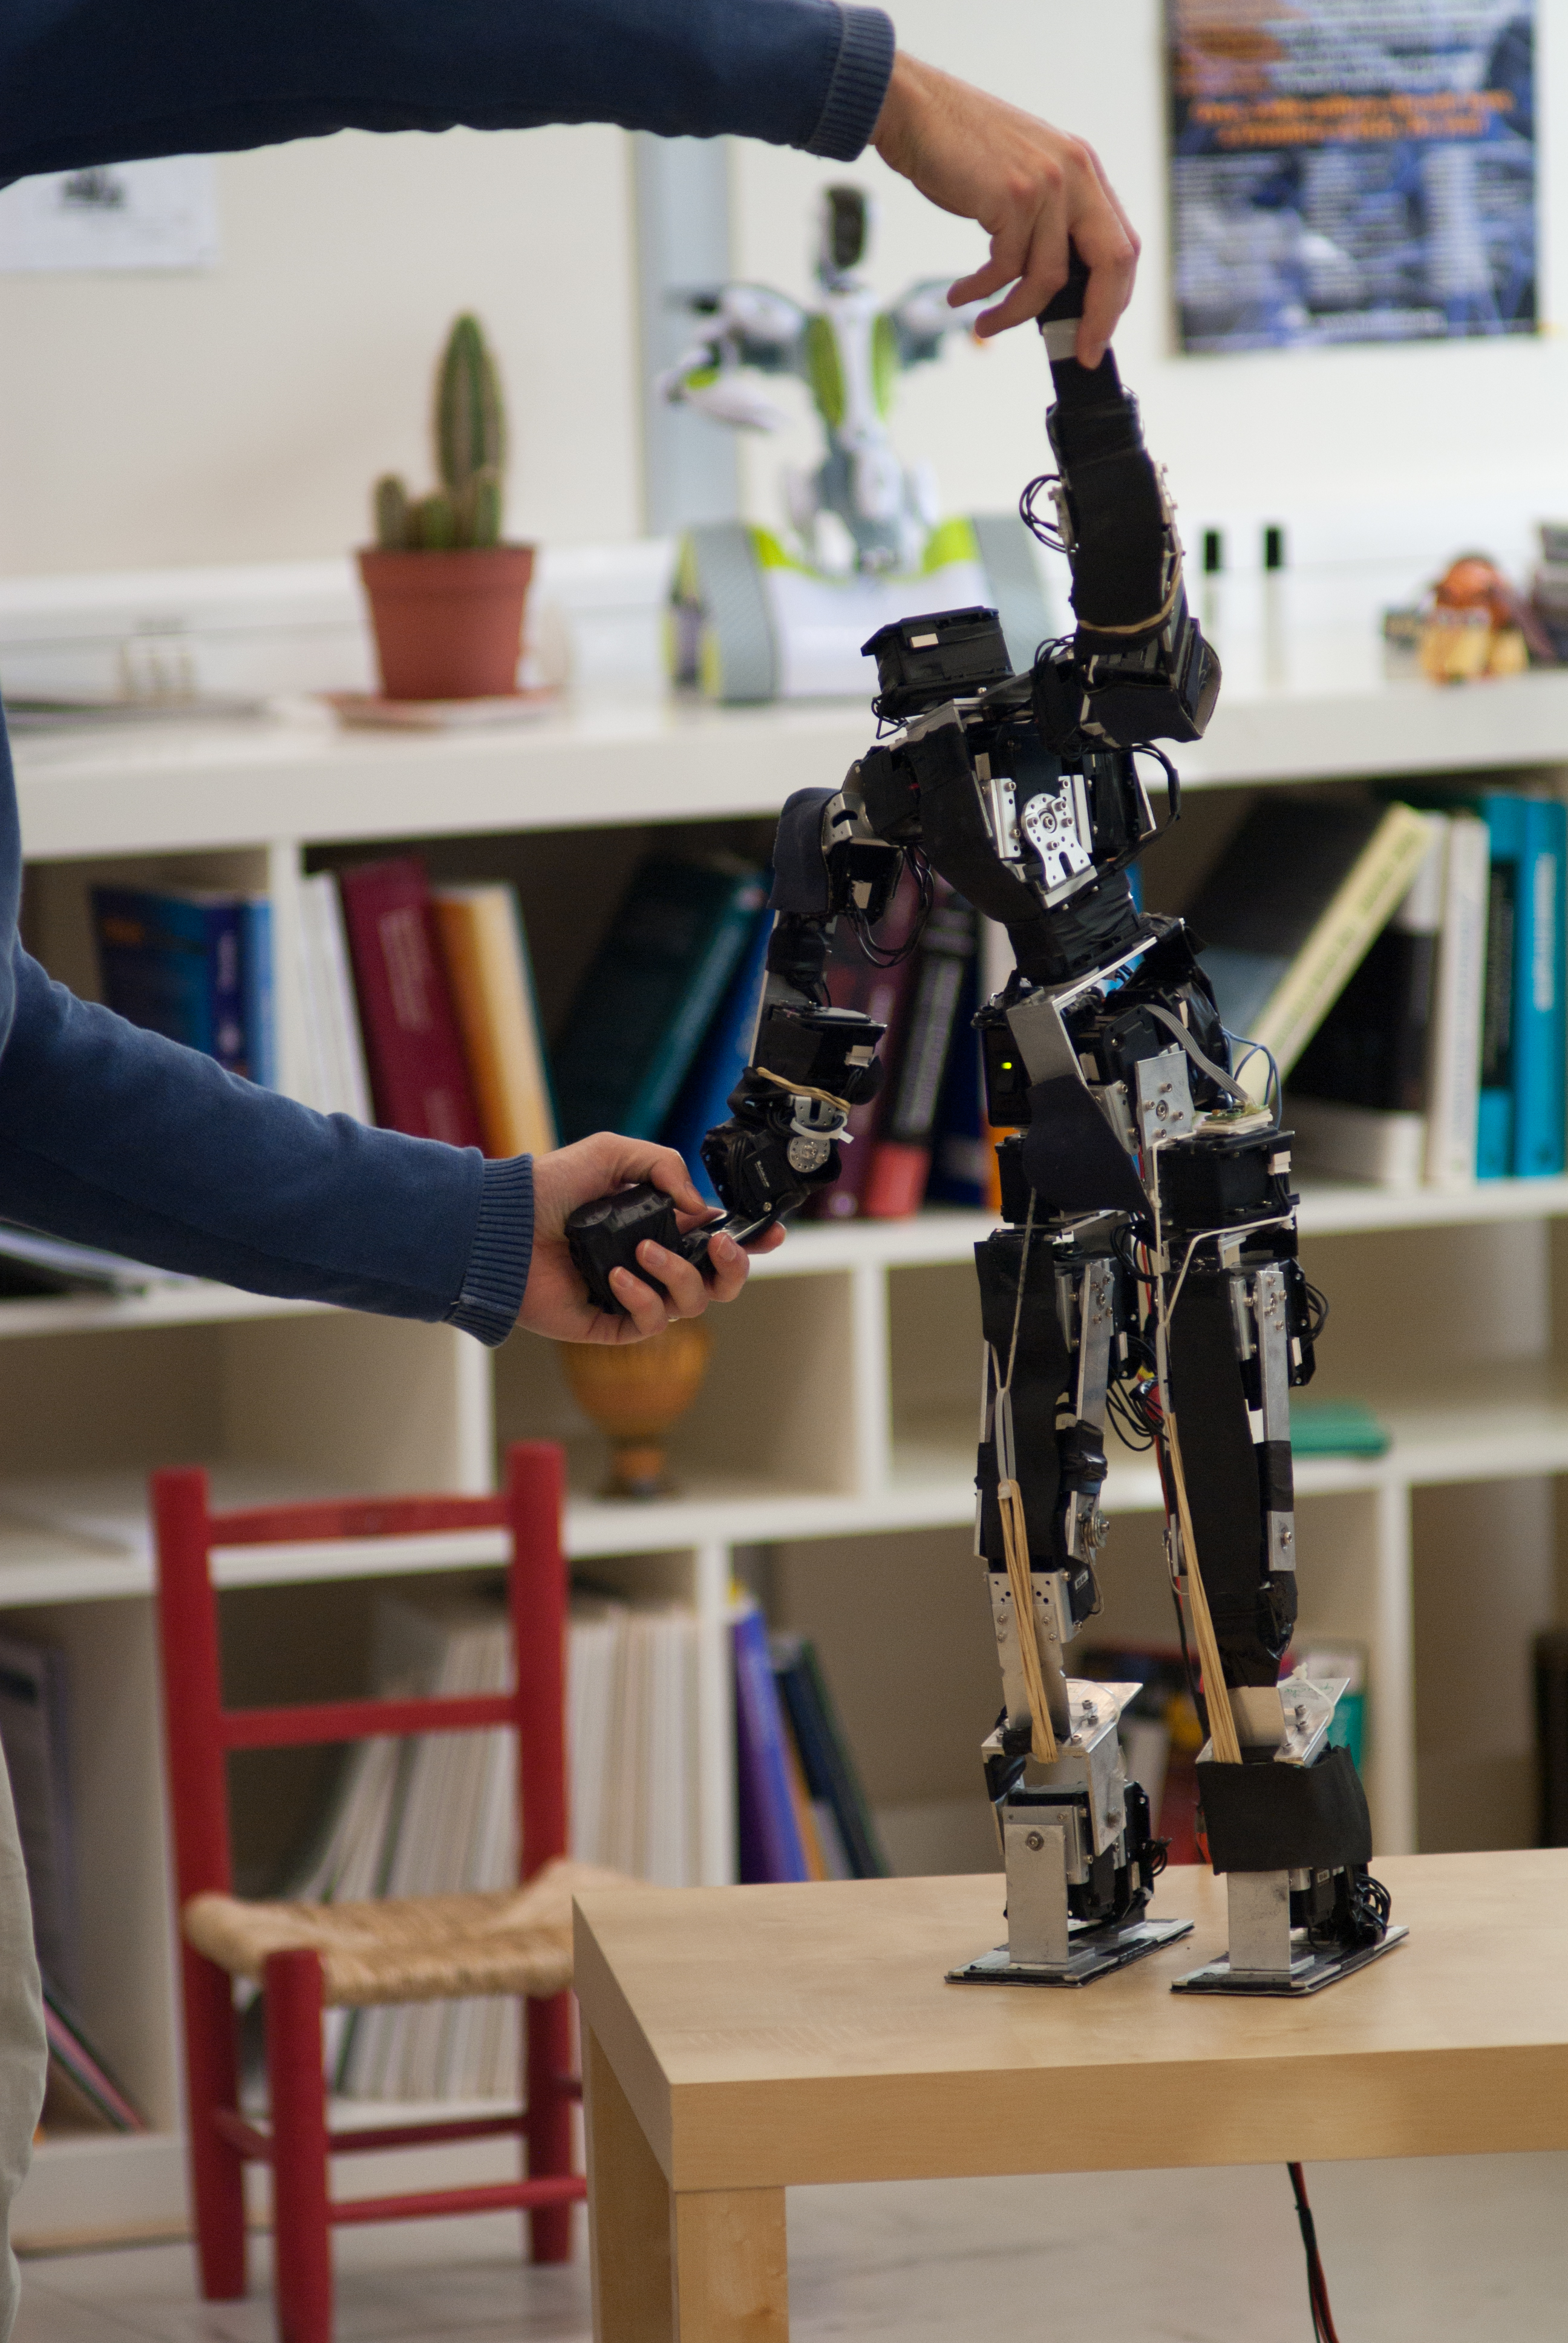
\includegraphics[width=0.9\linewidth]{../media/acroban2.jpg}
    \end{subfigure}
    \caption{\label{fig:robot_acroban} 
        Le robot Acroban, ancêtre de Sigmaban.
    }
\end{figure}

Le robot humanoïde Acroban, représenté sur la 
figure \ref{fig:robot_acroban}, est l'un des premiers robots 
conçus et construits par l'équipe Rhoban utilisant 
les servomoteurs Dynamixel.
Il peut être considéré comme l'ancêtre du robot Sigmaban.
Plus grand que Sigmaban, Acroban possède également plus de degrés de liberté, 
soit $26$ articulations. 
Ce robot à servi de plateforme expérimentale dans l'équipe 
\textit{FLOWERS} de l'INRIA 
(\cite{ly_acroban_2010}, \cite{lapeyre_maturational_2011},
\cite{ly_bio-inspired_2011}, \cite{oudeyer_exploring_2011}).
Des domaines variés comme l'interaction homme-robot, 
la \textit{compliance}\footnote{Mouvement souple, s'adaptant 
activement ou passivement au contact avec l'environnement.}
des mouvements (par exemple de la colonne vertébrale),
la robotique développementale ont été expérimentés.
Ce robot a de plus été utile à l'équipe pour appréhender les problématiques
posées par la mécatronique, les moteurs, le contrôle 
et la programmation des robots humanoïdes.
La locomotion de ce robot était fonctionnelle bien que peu rapide
en comparaison de sa taille.\\

\begin{figure}[htb]
    \centerfloat
    \begin{subfigure}{0.3\paperwidth}
        \centering
        \includegraphics[width=0.9\linewidth]{../media/sigmaban_1_0.jpg}
    \end{subfigure}
    \begin{subfigure}{0.3\paperwidth}
        \centering
        \includegraphics[width=0.9\linewidth]{../media/sigmaban_1_1.jpg}
    \end{subfigure}
    \begin{subfigure}{0.3\paperwidth}
        \centering
        \includegraphics[width=0.84\linewidth]{../media/sigmaban_1_2_crop.jpg}
    \end{subfigure}
    \newline
    \begin{subfigure}{0.3\paperwidth}
        \centering
        \includegraphics[angle=-90,width=0.9\linewidth]{../media/sigmaban_1_3.jpg}
    \end{subfigure}
    \begin{subfigure}{0.3\paperwidth}
        \centering
        \includegraphics[angle=-90,width=0.9\linewidth]{../media/sigmaban_1_4.jpg}
    \end{subfigure}
    \begin{subfigure}{0.3\paperwidth}
        \centering
        \includegraphics[width=0.915\linewidth]{../media/sigmaban_1_5_crop.jpg}
    \end{subfigure}
    \caption{\label{fig:robot_sigmaban_evolution} 
        Évolution du robot Sigmaban de gauche à droite et de haut en bas de 2011 à 2016.
    }
\end{figure}

De 2011 à 2017, la plateforme Sigmaban n'a pas cessé d'évoluer.
Son développement étant rythmé par la participation chaque année 
à la compétition RoboCup.
La figure \ref{fig:robot_sigmaban_evolution} retrace cette évolution et montre
l'apparence du robot année après année.
Les principales étapes de cette évolution dont j'ai été témoin et 
quelques fois acteur sont les suivantes :
\begin{itemize}
    \item Les premières versions de Sigmaban comportaient $22$ servomoteurs.
        Comme chez Acroban, deux articulations étaient présentes dans le dos
        du robot au dessus du bassin. 
        De plus, des amortisseurs (soit un degré de liberté non contrôlé) étaient 
        fixés au niveau des hanches du robot.
        Malgré l'intérêt de ces innovations mécaniques, elles ont été
        retirées en 2014 pour venir vers l'architecture mécanique \og classique \fg
        des robots humanoïde de la RoboCup avec $20$ servomoteurs.
        En raison du jeu mécanique supplémentaire induit par ces articulations, 
        cette architecture n'était pas en l'état suffisamment compétitive. 
        Sa marche était trop instable.
    \item Mise en place en 2014 d'une architecture logicielle pour le module de vision 
        basée sur un \textit{pipeline} de filtres (et \textit{OpenCV}).
        Les images de la caméra sont analysées successivement au travers d'un graphe 
        de traitements indépendants.
        Cette architecture rend le système plus facilement configurable, flexible
        et plus rapidement adaptable aux conditions visuelles d'un 
        nouvel environnement RoboCup.
    \item Entre 2014 et 2015, l'écriture du générateur de marche en boucle ouverte
        (\textit{IKWalk}) a permis d'améliorer la stabilité et la maniabilité 
        du déplacement du robot (voir section \ref{sec:walk}).
    \item Le renouvellement progressif à partir de 2015 des servomoteurs Dynamixel  
        remplace la gamme \textit{RX} par la gamme \textit{MX}.
        L'utilisation d'encodeurs magnétiques plus précis et moins sensibles 
        à l'usure mécanique que les potentiomètres améliore au fur et à mesure 
        la qualité des mouvements du robot.
    \item Le module de localisation basé sur un filtre particulaire 
        a commencé à être employé en 2015.
        Il s'appuie sur la détection des bases des poteaux de but ainsi 
        que sur les bordures du terrain pour situer le robot de manière absolue 
        lors d'un match de football robotique.
    \item Depuis 2015, les déplacements du robot sont intégrés par l'implémentation 
        d'un modèle géométrique direct (section \ref{sec:modele_direct}) 
        et de la reconstruction de l'état du robot (section \ref{sec:estimation_etat})
        à partir de ses capteurs.
        L'information de l'odométrie est particulièrement importante 
        pour le processus de localisation et d'asservissement des ordres de la marche.
    \item Le développement des capteurs de pression en 2015 sous les pieds des robots
        est concomitant à l'introduction de l'herbe artificielle comme surface de marche
        par la RoboCup.
        Pour réduire une grande partie de l'effet de déstabilisation de l'herbe artificielle, 
        des crampons sont ajoutés aux pieds des robots.
        Les capteurs de pression y sont directement attachés. 
        Ces capteurs sont essentiels à l'odométrie (section \ref{sec:odometry_pressure}) 
        et au processus de stabilisation de la marche.
    \item Une refonte de toute l'architecture logicielle a été entreprise en 2015.
        Précédemment, le programme principal contrôlant le robot comportait, à la manière 
        de \textit{ROS} (\textit{Robot Operating System}), 
        plusieurs modules indépendants et communicant par envoi de messages.
        Une interface graphique écrite en C\# permettait de contrôler et 
        de superviser les robots.
        À ceci a été préféré une architecture purement monolithique, simplifiant
        la communication des différents modules.
        Une bibliothèque de configuration, de monitorage et de contrôle du robot a été
        développée (\textit{RhIO}) avec un \textit{shell} (textuel) comme interface 
        utilisateur.
    \item En 2016, la conception d'une nouvelle carte électronique a
        séparé la communication avec les servomoteurs en trois bus séries distincts.
        Grâce également à la réimplémentation de la gestion de la communication bas niveau 
        au niveau de l'ordinateur embarqué (bibliothèque \textit{RhAL}, 
        voir section \ref{sec:other_works})
        il a été possible de doubler la fréquence de la boucle de lecture-écriture 
        de $50$~Hz à $100$~Hz.
        Cette augmentation de fréquence a amélioré la fluidité de tous les mouvements.
    \item La \textit{webcam} au niveau de la tête du robot a été remplacée en 2016
        par une caméra dite \og industrielle \fg. 
        Ces caméras ont pour principal intérêt une capture de l'image par 
        \textit{global shutter} plutôt que par \textit{rolling Shutter}.
        Tous les pixels du capteur enregistrent l'image au même moment plutôt que
        ligne par ligne.
        Ceci réduit grandement le flou dû aux mouvements de la tête du robot.
        De plus, elles sont plus finement paramétrables 
        (balance des couleurs, vitesse d'obturation, ...).
        
        En 2017, l'API propriétaire (en remplacement de \textit{v4l2}) a permis une meilleure 
        maitrise des horodatages de capture des images.
        Ce qui a amélioré la synchronisation temporelle entre la caméra 
        et les autres capteurs\footnote{Connaitre avec exactitude la valeur des capteurs 
        (encodeurs, IMU) du robot au moment de la prise d'image est crucial pour 
        la précision du calcul de la position cartésienne relative des objets détectés dans l'image. 
        La difficulté réside dans la synchronisation des horodatages
        entre les lectures bas niveau sur le bus de communication série et le pilote de la caméra.}.
        D'une connectique USB 3.0 en 2016, nous sommes passés en 2017 
        à une liaison ethernet entre la caméra et l'ordinateur embarqué
        pour des raisons d'interférences électromagnétiques entre 
        le câble USB 3.0 et la communication radio WiFi.
        Enfin, le choix personnalisé de la lentille (grand angle ou petit angle)
        laisse plus de liberté quand à la stratégie de scan et de détection
        (compromis entre l'ouverture angulaire, la résolution de l'image par degré, 
        la déformation de l'image et le temps de balayage du terrain).
    \item L'utilisation en 2017 d'un apprentissage par un réseau de neurones profond 
        pour la détection de la balle et des buts a radicalement amélioré la vision du robot.
        Les réseaux de neurones ont apporté une plus grande robustesse aux conditions lumineuses, 
        à l'occlusion partielle des objets, moins de faux positifs ainsi 
        qu'une plus grande portée de détection.
    \item Le développement d'une nouvelle marche en 2017, la \textit{QuinticWalk} toujours
        dans l'espace cartésien mais basée sur des splines polynomiales de degré $5$
        a apporté une meilleure stabilité du déplacement, particulièrement importante 
        sur le plus grand robot (voir section \ref{sec:other_works}).\\
\end{itemize}

\begin{figure}[htb]
    \centerfloat
    \begin{subfigure}{0.35\paperwidth}
        \centering
        \includegraphics[width=0.7\linewidth]{../media/grosban_1_0.jpg}
    \end{subfigure}
    \begin{subfigure}{0.35\paperwidth}
        \centering
        \includegraphics[width=1.0\linewidth]{../media/grosban_1_1.png}
    \end{subfigure}
    \caption{\label{fig:robot_grosban} 
        Le robot Grosban, une version plus grande et plus puissante de Sigmaban.
        À gauche, la première version de $90$~cm en 2015 et à droite, 
        la deuxième version plus petite à $75$~cm en 2016.
    }
\end{figure}

\begin{figure}[htb]
    \centerfloat
    \includegraphics[width=0.4\linewidth]{../media/sigmaban_1_6.png}
    \includegraphics[width=0.4\linewidth]{../media/grosban_1_2.png}
    \caption{\label{fig:robot_sigmaban_2017} 
        Version 2017 du robot Sigmaban à gauche et Sigmaban+ 
        (évolution de Grosban) à droite.
    }
\end{figure}

En plus de la plateforme Sigmaban, un robot plus grand, Grosban est également
expérimenté par l'équipe (figure \ref{fig:robot_grosban}).
La première version en 2015 de $90$~cm de haut était trop grande.
Les imperfections (jeux mécaniques, défauts d'asservissement) en regard de sa taille
étaient telles que sa marche était difficilement stable ; et les pas chassés latéraux 
fortement bridés. Ce robot n'était quasiment plus omnidirectionnel.
En 2016 et 2017, sa taille a été réduite, améliorant son rapport poids 
(bras de levier) puissance.
Après une nouvelle conception mécanique et l'écriture
d'un nouveau mouvement de marche plus stable (\textit{QuinticWalk}), ce robot
(rebaptisé Sigmaban+) est devenu en 2017 le meilleur joueur de l'équipe.
Son déplacement étant en effet plus rapide et son tir plus puissant.

Les versions 2017 des robots Sigmaban et Sigmaban+ sont dépeints
sur la figure \ref{fig:robot_sigmaban_2017}.

\subsection{Description des composants mécaniques et électroniques}

Cette section décrit rapidement les principaux composants
matériels constitutifs de la plateforme Sigmaban dans sa version 2017.
Le robot possède un total de $20$ articulations chacune contrôlée
par un servomoteur. Chaque jambe en comporte $6$, chaque bras $3$
ainsi que $2$ articulations dans le cou du robot.
La liste de ces degrés de liberté est donnée dans la section \ref{sec:model_conventions}.
Le robot mesure $57$~cm de haut dans sa posture de référence ; 
les jambes et les bras tendus.
Sa masse vaut environ $4.2$~Kg\footnote{La masse totale du robot ne peut pas être simplement 
déduite de la somme des masses de ses composants principaux et des pièces mécaniques 
d'après les schémas de conceptions.
Il s'avère que la visserie acier ainsi que le câblage électrique représentent une part
très significative aux alentour de $1$~Kg de la masse totale du robot.}.

\subsubsection{Capteurs de pression\label{sec:robot_pressure_sensors}}

\begin{figure}[htb]
    \centerfloat
    \includegraphics[width=0.8\linewidth]{../media/pressures1.png}
    \vspace{0.1cm}
    \newline
    \includegraphics[width=0.8\linewidth]{../media/pressures2.png}
    \caption{\label{fig:robot_pressures} 
        La première (2015--2016) (en haut) et seconde (2017) (en bas) versions 
        des capteurs de pression conçues et fabriquées au sein de l'équipe.
    }
\end{figure}

La figure \ref{fig:robot_pressures} montre la première et la seconde version
des capteurs de pression sous les pied du robot.
Ces capteurs sont basés sur l'utilisation de jauges de déformation.
Il s'agit de pièces mécaniques en métal dont les déformations infinitésimales
sont mesurées par un réseau de résistances variables selon l'élongation.
Plus précisément, une tension électrique est mesurée, souvent au travers
d'un pont de Wheatstone, liée à la déformation de la pièce mécanique.
La géométrie de la pièce et la position des jauges de déformation sont 
savamment choisies pour obtenir une mesure \textit{différentielle} de l'élongation.

Pour pouvoir fonctionner, ces jauges de déformation sont mécaniquement
intégrées aux quatre crampons sous les pieds du robot.
L'intérêt des crampons est double.
Tout d'abord, ils ont été introduit après que le règlement 
de la RoboCup ait remplacé la surface de marche d'une fine moquette par 
de l'herbe artificielle d'une épaisseur de $3$~cm.
En comparaison de la taille et du poids du robot, cette épaisseur molle
et irrégulière entraine de très fortes perturbations de la stabilité des robots.
L'utilisation de crampons s'enfonçant dans l'herbe jusqu'au sol dur stabilise
et réduit grandement l'effet de cette surface.
De plus, le poids du robot au lieu d'être réparti sur toute
la surface d'un pied plat se concentre sur ces quatre points.
Les forces transmises du robot au sol sont alors bien plus faciles
à mesurer.

L'utilisation des jauges de déformation alliée à cette intégration mécanique 
s'est révélée permettre une mesure des forces de pression
bien plus précise, résiliente et mécaniquement robuste que son équivalent 
basé sur les FSR\footnote{Les FSR sont par exemple présents dans les pieds 
des robots NAO. Cependant, plusieurs auteurs (\cite{alcaraz-jimenez_robust_2013}) 
semblent confirmer que le bruit
de mesure rend délicat leur utilisation autrement que part une lecture purement binaire.}.
Les FSR (\textit{Force-Sensing Resistor}) sont des matériaux polymères dont
la résistance électrique varie directement selon les forces de pression 
qui leurs sont appliquées.
Contrairement aux jauges de déformation, ils ne mesurent 
que la force les traversant, les écrasant.
De nombreuses expérimentations réalisées par l'équipe ont indiqué que 
leur intégration mécanique était difficile et mécaniquement peu solide.
En effet, il est particulièrement délicat d'arriver à faire traverser 
dans ces capteurs l'intégralité des forces de pression entre le sol 
et le pied du robot.

Grâce à ces capteurs présentés plus en détail par \cite{ProjectsWorkshopHumanoids2015} et
\cite{PassaultThesis}, la répartition du poids du robot sur chaque pied
ainsi qu'une estimation du centre de pression\footnote{L'information du centre de pression
lié au ZMP est de première importance pour l'étude de la marche du robot.} peuvent être obtenues.
Ces capteurs sont essentiels à l'estimation de l'odométrie (section \ref{sec:odometry_pressure})
et de la procédure de stabilisation de la marche (section \ref{sec:walk_stabilization}).

\subsubsection{Ordinateur embarqué et caméra}

\begin{figure}[htb]
    \centerfloat
    \begin{subfigure}{0.35\paperwidth}
        \centering
        \includegraphics[width=0.8\linewidth]{../media/fitlet.jpg}
    \end{subfigure}
    \begin{subfigure}{0.35\paperwidth}
        \centering
        \includegraphics[width=0.8\linewidth]{../media/camera_blackfly.jpg}
    \end{subfigure}
    \caption{\label{fig:robot_pc_camera} 
        Ordinateur embarqué \textit{fitlet-i} de \textit{CompuLab} (à gauche) et 
        la caméra industrielle ethernet \textit{blackfly} de \textit{PointGrey} (à droite).
    }
\end{figure}

Le choix de l'ordinateur embarqué est fortement conditionné par sa taille
et son poids puisqu'il est intégré au niveau du dos du robot.
L'ordinateur choisi est le \textit{fitlet-i}\footnote{\url{http://www.fit-pc.com/web/products/fitlet/}}
de \textit{CompuLab} représenté sur la gauche de la figure \ref{fig:robot_pc_camera}.
Le processeur AMD A4 Micro-6400T (1.0 GHz) suit une architecture x86 64-bits 
et possède 4 cœurs de calculs.
L'ordinateur embarque un disque SSD robuste aux nombreux chocs que subit le robot
et un système Linux (Debian) y est installé.\\

La caméra industrielle couleur 
\textit{blackfly GigE}\footnote{\url{https://www.ptgrey.com/blackfly-usb3-vision-cameras}}
de l'entreprise \textit{Point Grey} est fixée au niveau de la tête du robot.
Elle est représentée sur la droite de la figure \ref{fig:robot_pc_camera}.
Son capteur fonctionne par \textit{global shutter} ou obturateur global, 
et capture l'intégralité des pixels de l'image au même moment.
Diminuer le flou des images est important car avec l'utilisation de \textit{webcams}
et sans \textit{global shutter}, il arrivait qu'un tiers des images soit
inexploitable en raison du flou.
Pour réduire le flou au maximum, le temps d'obturation est réduit autant que possible
et la perte de luminosité est compensée par l'augmentation 
du gain des capteurs\footnote{L'augmentation du gain et donc la réduction 
du temps d'obturation est limitée par le bruit statique des capteurs.}.
La connectique ethernet a deux intérêts. 
Premièrement, le connecteur est plus robuste aux chocs que le connecteur USB
et souffre donc moins de déconnections passagères.
Deuxièmement, il n'y a pas d'interférence électromagnétique avec la bande
de fréquences utilisée par la communication WiFi (voir la note d'Intel \cite{USB3Wifi}).

Le choix de la lentille s'est porté sur une petite ouverture angulaire de $67$ degrés en largeur.
Les très faibles déformations optiques de cette lentille n'ont pas besoin d'être compensées.
Contrairement à une lentille grand angle, elle permet par son \og zoom \fg de 
repérer la balle à longue distance sur le terrain mais ne perçois qu'une petite partie de celui ci.
Le mouvement de recherche (scan) de la balle nécessite alors des mouvements de têtes plus 
lent et plus réguliers.

\subsubsection{Servomoteurs Dynamixel}

\begin{figure}[htb]
    \centerfloat
    \begin{subfigure}{0.3\paperwidth}
        \centering
        \includegraphics[width=0.8\linewidth]{../media/dynamixel1.jpg}
    \end{subfigure}
    \begin{subfigure}{0.3\paperwidth}
        \centering
        \includegraphics[width=0.95\linewidth]{../media/dynamixel2.jpg}
    \end{subfigure}
    \begin{subfigure}{0.3\paperwidth}
        \centering
        \includegraphics[width=0.95\linewidth]{../media/dynamixel3.jpg}
    \end{subfigure}
    \caption{\label{fig:robot_dynamixel} 
        Photos du servomoteur commercial \textit{MX-64} 
        \textit{Dynamixel} de \textit{Robotis}.
    }
\end{figure}

Le mouvement du robot est créé par ses actuateurs au niveau de chaque articulation.
Les servomoteurs commerciaux \textit{Dynamixel} de l'entreprise sud-coréenne \textit{Robotis} 
(visibles sur la figure \ref{fig:robot_dynamixel})
sont très répandus dans la communauté des robots humanoïde de la RoboCup.
Ces servomoteurs ont pour avantages leur disponibilité commerciale \og sur l'étagère \fg, 
leur protocole de communication série et la qualité de leur intégration mécanique
et électronique\footnote{Voir la documentation constructeur : 
\url{http://support.robotis.com/en/product/actuator/dynamixel/mx_series/mx-64at_ar.htm}}.
Ils sont disponibles selon deux gammes, \textit{RX} et \textit{MX} et plusieurs 
modèles.
La série \textit{MX} est la plus récente et aujourd'hui la plus utilisée sur nos robots.
La série \textit{RX} est obsolète mais équipe encore un de nos robots Sigmaban en 2017.
La suite se concentre sur la description 
des modèles \textit{MX}\footnote{Couple à vitesse nulle maximum 
à $12$~V d'après les spécifications constructeur : 
\textit{MX-28} $2.5$~N.m, \textit{MX-64} $6.0$~N.m, \textit{MX-106} $8.4$~N.m}.

Les performances motrices de nos robots sont intimement liées aux capacités 
de leurs servomoteurs. Leur bonne connaissance est essentielle.
Les servomoteurs Dynamixel existent en différents modèles de couple maximal croissant.
Sur la plateforme Sigmaban, les $12$ articulations des jambes, plus sollicitées, 
sont équipées de moteurs \textit{MX-64} alors que le haut du corps devant fournir moins
de couple utilisent des moteurs \textit{MX-28}.
La plateforme Sigmaban+ (Grosban) utilise quant à elle des \textit{MX-106} pour le bas du corps et
des \textit{MX-64} pour le haut du corps.

Ces servomoteurs sont constitués d'un moteur à courant continu, 
d'une boite d'engrenages planétaires assurant la réduction de la vitesse du moteur
en couple, d'un encodeur de position fixé directement sur l'arbre
de sortie ainsi que d'une électronique de contrôle (régulateur de tension,
microcontrôleur et pont en H).
Contrairement aux versions \textit{RX} qui se basaient sur des potentiomètres, 
les encodeurs de position des \textit{MX} sont magnétiques (effet Hall).
Mécaniquement beaucoup plus robustes à l'usure, leur résolution est également meilleure
et atteint environ $0.08$ degrés contre $0.3$ degrés pour les \textit{RX}.
Il est important de bien noter que ces encodeurs mesurent la position angulaire
absolue de l'arbre de sorti, après la boite d'engrenages.
Leur tension d'alimentation nominale est aux alentours des $12$~V.

Contrairement aux servomoteurs analogiques \og hobbyistes \fg,
la communication avec l'électronique de contrôle des moteurs 
se fait au travers d'un protocole série. 
Plusieurs moteurs peuvent ainsi être connectés à la suite sur le même bus.
Ce protocole permet de lire et d'écrire la valeur de registres au sein de
la mémoire du microcontrôleur.
De nombreuses informations comme la position lue par l'encodeur, 
la tension d'alimentation ou encore la température du moteur peuvent 
ainsi être accédées. 
L'expérience a aussi montré que certaines de ces informations 
telles que la vitesse du moteur ou encore la mesure du courant électrique
n'étaient pas fiables et ne pouvaient être en pratique utilisées.

Le principal mode de contrôle du servomoteur s'utilise en écrivant 
dans un registre la position angulaire cible de l'arbre de sortie.
Cette commande de référence ou consigne de position est suivie
tant qu'une autre position n'est pas précisée.
L'ordre de position est alors perpétuellement mis à jour à la fréquence
de la boucle de lecture-écriture du bas niveau, soit $100$~Hz.
L'asservissement de cette consigne repose sur un simple contrôle
proportionnel dont le coefficient est configurable.

Outre la position quasiment monopolistique de l'entreprise \textit{Robotis}
sur ce petit marché, le principal défaut de ces servomoteurs 
tient à la fermeture complète du code source de leurs contrôleurs.
Un effort de rétro-ingénierie est souvent nécessaire pour affiner
la compréhension de certains comportements limites du contrôleur.
C'est dans cette optique que Rémi Fabre a entrepris l'implémentation libre et ouverte
du contrôleur alternatif 
\textit{Dynaban}\footnote{\url{https://github.com/RhobanProject/Dynaban}} 
pour les moteurs \textit{MX-64}.
Ce projet a apporté à l'équipe une profonde compréhension 
du fonctionnement de ces servomoteurs.
Ces travaux ont de plus donnés lieu à l'expérimentation d'un contrôle 
prédictif en couple décrit dans \cite{DynabanRoboCup2016}.

\subsubsection{Carte électronique bas niveau}

\begin{figure}[htb]
    \centerfloat
    \includegraphics[type=pdf,ext=.pdf,read=.pdf,width=0.6\linewidth]{../schema/3bus}
    \caption{\label{fig:robot_board} 
        Carte électronique bas niveau.
        La carte divise en trois bus séparés (haut du corps, jambe gauche et jambe droite)
        la communication avec les moteurs et capteurs.
    }
\end{figure}

La carte électronique bas niveau conçus au sein de l'équipe est représentée 
sur la figure \ref{fig:robot_board}.
Elle est au centre de la communication entre l'ordinateur embarqué et des autres composants
électroniques : les servomoteurs, la centrale inertielle et les capteurs de pression.
Cette carte est construite autour du microcontrôleur STM32 sous l'architecture 
ARM Cortex M3 ($72$~MHz) et intégré à la sous carte d'évaluation \textit{maple mini}.

La communication entre l'ordinateur et le microcontrôleur se fait 
au travers d'une liaison USB.
Le microcontrôleur est ensuite relié aux servomoteurs ainsi qu'aux
capteurs de pression par trois bus séries TTL (\textit{Transistor-Transistor Logic}).
Plus précisément, ces bus travaillent en parallèle :
chacune des deux jambes est branchée sur un bus distinct 
et le troisième bus couvre les servomoteurs des bras et de la tête.
Le microcontrôleur assure la répartition des paquets de communication
sur les trois bus puis les regroupe lors de la transmission USB.
Cette répartition permet à la boucle de lecture de tous les capteurs
et d'écriture des ordres moteurs d'atteindre une fréquence aux alentours
des $100$~Hz\footnote{La fréquence
effective est dépendante de la taille des données échangées à chaque cycle de 
lecture-écriture avec les servomoteurs. Les registres lus et écrits sont ainsi
limités au strict nécessaire.}.
Les bus séries transmettent à la fréquence d'un million de bauds par seconde.

La centrale inertielle \textit{GY-85}, $9$ axes, rassemble trois accéléromètres,
trois gyromètres et trois magnétomètres alignés avec les axes de l'espace.
Cette dernière est directement reliée au microcontrôleur par un bus SPI.
Il s'avère que la centrale peut être interrogée à une plus haute fréquence
que la fréquence de la boucle de lecture-écriture entre le microcontrôleur et l'ordinateur.
Le microcontrôleur sert alors de mémoire tampon. Les mesures des accéléromètres et 
des gyromètres sont transférées sur l'ordinateur embarqué puis mélangées par un algorithme de filtrage
(voir le filtrage à la section \ref{sec:estimation_etat}).

\subsection{De nombreuses imperfections\label{sec:robot_flaws}}

On considère par définition comme imperfection,
tout comportement du robot réel n'étant pas en accord
avec les prédictions théoriques du modèle classique
de la dynamique des solides rigides.
Dans de très nombreux cas, la conception mécanique et électrique des 
robots a pour objectif de réduire les sources d'imperfections 
afin de faire coïncider le comportement dynamique du robot avec celui 
de la théorie mathématique.

Beaucoup de robots humanoïdes suivent cette approche.
On peut par exemple mentionner \textit{ASIMO}, \textit{HRP-2} pour les grands
robots, les jambes du \textit{iCub} de taille intermédiaire 
et \textit{HOAP-3} de même taille que Sigmaban.
Typiquement, leur système de réduction n'utilise pas de boites à engrenages
planétaires mais plutôt des réducteurs harmoniques éliminant tout jeu mécanique.
Leur servomoteurs sont spécifiquement conçus pour leur architecture mécanique très précise.

En comparaison, nos petits robots et plus généralement les robots humanoïdes présents
aux compétitions RoboCup présentent de nombreux défauts.
Tout d'abord, leur petite taille limite fortement les possibilités 
d'intégration mécanique.
Il est par exemple bien plus délicat de développer 
des servomoteurs non industriels adaptés à cette taille.
Mais bien que plus petits, ils sont également beaucoup moins fragiles.
De nombreuses expérimentations menées sur les petits robots 
ainsi que les conditions de jeu présentes à la compétition
RoboCup sont souvent violentes (chutes fréquentes, collisions). 
Peu de grands robots pourraient supporter (sans palan) de telles 
conditions \footnote{En contre exemple, on peut mentionner le robot \textit{Atlas} 
de \textit{Boston Dynamics}. À noter cependant que ses actuateurs sont hydrauliques.}.
À noter que pour compenser leur perte en précision du contrôle moteur, 
la surface des pieds des petits robots tend souvent à
être plus grande (en comparaison de leur taille) que sur 
les grands robots humanoïdes.

Dans la suite, quatre sources d'imperfections du comportement du robot Sigmaban 
et dont les impacts se sont révélés importants pour l'odométrie, la synthèse de
mouvements ou la simulation sont détaillées.

\subsubsection{Les déformations mécaniques}

\begin{figure}[htb]
    \centerfloat
    \begin{subfigure}{0.4\paperwidth}
        \centering
        \includegraphics[width=1.0\linewidth]{../media/torsion_meca1.jpg}
    \end{subfigure}
    \begin{subfigure}{0.4\paperwidth}
        \centering
        \includegraphics[width=1.0\linewidth]{../media/torsion_meca2.jpg}
    \end{subfigure}
    \caption{\label{fig:robot_meca_twist} 
        Torsion des pièces mécaniques au niveau du bras (à gauche) 
        et de la jambe du robot Sigmaban (à droite).
    }
\end{figure}

En théorie, la géométrie du robot est parfaitement connue.
Les pièces mécaniques sont conçues et dessinées par ordinateur.
L'usinage est réalisée par découpe de plaques d'aluminium à l'aide 
d'une machine à commande numérique.
Les pièces sont alors finalisées et assemblées aux servomoteurs.

Malheureusement, ces pièces métalliques se déforment.
Deux exemples de ces déformations sont visibles sur la figure \ref{fig:robot_meca_twist}.
La principale cause de ces déformations sont les nombreuses chutes du robot,
courantes au cours des diverses expérimentations et des matchs de football robotique.
Lors des compétitions RoboCup, on peut également incriminer le transport en valise
mais surtout les collisions avec les autres robots.
À noter que des tests ont commencés à être effectués dans l'équipe pour remplacer
l'aluminium par des plaques de fibres de carbone, cassantes mais non déformables.
En plus des déformations des segments métalliques liant les moteurs entre eux, 
il s'est avéré que les arbres de sorties des servomoteurs pouvaient également
présenter des torsions (hélicoïdales).
Ces torsions, physiquement invisibles sans démonter le moteur, 
ont pour effet d'ajouter plusieurs degrés à l'angle de l'articulation.
Ceci créant une erreur angulaire statique car non mesurée par les encodeurs 
de position.

Toutes ces déformations ont pour conséquences d'augmenter l'erreur entre
notre modèle géométrique du robot (voir section \ref{sec:modele_direct} pour la définition)
et sa géométrie réelle.
À noter que la non rigidité des pièces mécaniques est ici négligeable
au regard des distances et des autres sources d'imperfections.
Les erreurs du modèle géométrique direct affecte notre perception 
de l'état du robot construit à partir de ses capteurs.
Par exemple, le modèle géométrique direct permet d'estimer l'orientation de
la caméra dans le repère égocentrique du robot.
Cette orientation est nécessaire pour calculer à quelle distance du robot 
se trouvent les objets détectés par l'analyse des images de la caméra.
Les chutes répétées du robot sur son cou déforment la géométrie des pièces,
faussent les calculs de distance et ainsi altèrent la localisation du robot sur le terrain.
À l'inverse, les erreurs du modèle géométrique inverse entraine des erreurs
de contrôle des jambes.
Typiquement, les pieds ne sont plus à plat par rapport au sol pendant la marche
et déstabilisent le robot.
Ces déformations modifient également à la marge sa dynamique.

\subsubsection{Le jeu des engrenages}

\begin{figure}[htb]
    \centerfloat
    \begin{subfigure}{0.4\paperwidth}
        \centering
        \includegraphics[type=pdf,ext=.pdf,read=.pdf,width=1.0\linewidth]{../schema/backlash_meca}
    \end{subfigure}
    \begin{subfigure}{0.4\paperwidth}
        \centering
        \includegraphics[type=pdf,ext=.pdf,read=.pdf,width=1.0\linewidth]{../schema/backlash_function}
    \end{subfigure}
    \caption{\label{fig:robot_backlash} 
        Représentation conceptuelle du phénomène du jeu mécanique des servomoteurs (à gauche) 
        et sa modélisation classique (à droite).
    }
\end{figure}

Outre les déformations, la deuxième source d'imperfections
réside dans le jeu mécanique (\textit{backlash}) des servomoteurs.
Le système de réduction des servomoteurs est composé de plusieurs
engrenages. Transmettant le mouvement du moteur à courant continu
vers l'arbre de sortie, ils diminuent la vitesse de rotation
tout en augmentant le couple exercé.
Quasiment inexistant quand le servomoteur est neuf, le jeu s'accroit
rapidement avec le temps d'utilisation.
La qualité d'un même mouvement (suivi de la trajectoire, fluidité)
peut être significativement différent si exécuté sur un robot \og neuf \fg,
et sur un robot ayant déjà deux ans (et deux participations à la RoboCup).

Le jeu est qualitativement facile à détecter et à estimer.
Une analogie mécanique, schématisée sur la gauche de la figure \ref{fig:robot_backlash},
décrit le phénomène : il existe un intervalle angulaire dans lequel 
l'arbre de sortie du servomoteur bouge beaucoup plus facilement.
Dans cet intervalle, les forces de frottements et l'inertie des parties mobiles
sont très faibles.
L'arbre de sortie bouge mais ni les engrenages, ni le moteur électrique ne sont
mis en rotation.
Quand l'arbre de sortie arrive en butée sur l'un des cotés de cet intervalle,
les engrenages et le moteur commencent alors à tourner et sont entrainés.
Une forte discontinuité des frottements et de l'inertie (qui augmentent) est ressentie.
Un choc (inélastique) pourrait même être considéré.
Tant que l'arbre reste en butée, le servomoteur se comporte alors \og normalement \fg.
Le jeu ne réapparait que lorsque le contact est rompu par la différence 
entre les forces externes s'appliquant sur l'arbre et les forces internes 
(moteur électrique, frottements, inertie) agissant sur les engrenages.

Il est important de remarquer que ce jeu mécanique est bien \textbf{mesuré} par
les encodeurs des servomoteurs car ces derniers sont liés à l'arbre de sortie.
En revanche, la position angulaire relative de l'arbre dans l'intervalle du jeu
n'est pas observable car interne aux engrenages et constitue le principal
\textbf{état caché} du système mécanique.

Ce jeu est supposé\footnote{Le démontage et la comparaison de deux servomoteurs, l'un neuf
et l'autre usé n'a pas encore été proprement effectué.} venir de deux phénomènes.
Premièrement, l'usure de la matière augmente avec le temps l'espace présent 
entre les dents des engrenages.
Dans les cas extrêmes, une de ces dents casse et le servomoteur devient
alors difficilement utilisable.
Deuxièmement, il est possible que les trous de fixation dans la coque en plastique
des axes de rotation des engrenages deviennent avec le temps ovoïdes.
Une dernière particularité de ce jeu est qu'il est non uniforme dans l'espace angulaire.
En effet, certaines positions articulaires et notamment les zones d'usures courantes sont
particulièrement affectées par un intervalle de jeu plus grand.
Ces zones correspondent typiquement à celles de la posture de marche du robot.
Ceci tend à incriminer le dernier engrenage, avant l'arbre de sortie.

Ce phénomène de jeu mécanique à deux principaux effets néfastes.
Tout d'abord, il dégrade la qualité de l'asservissement de la position 
angulaire des servomoteurs.
Comme le montre la fonction dessinée sur la droite de la figure \ref{fig:robot_backlash},
le jeu correspond à une zone dans laquelle le moteur électrique ne peut plus 
agir sur la position angulaire de l'arbre de sortie.
Cet effet est surtout présent au début du mouvement et lors
des changements de sens de rotation des articulations.
D'autre part, le jeu affecte gravement la dynamique du robot. 
De l'extérieur, l'articulation apparait comme quasiment libre dans un cône
autour de sa position cible.
Pire, ces cônes s'accumulent sur toutes les articulations placées selon le même axe.
Cette \og compliance \fg engendre comme des degrés de liberté non contrôlés qui 
tendent à induire des tremblements et des oscillations parasites du système mécanique.
Par exemple, le buste du robot en posture de marche peut toujours 
légèrement translater et s'incliner librement par rapport aux jambes.
Son comportement peut ainsi faire penser dans une certaine mesure à celui d'un double 
pendule inversé non contrôlé\footnote{Cet effet était fortement amplifié par 
la présence d'articulations supplémentaires au dessus du bassin dans les 
premières versions de Sigmaban.}.

Pour donner un exemple quantitatif, le robot Sigmaban est mis en posture de marche statique
(chevilles, genoux et hanches légèrement pliés, le buste incliné vers l'avant).
Dans cette posture, le buste du robot est faiblement déplacé manuellement 
dans l'axe avant-arrière tout en restant dans les zones de jeu des servomoteurs
des jambes (chevilles, genoux et hanches en tangage).
Ces zones sont facilement ressenties manuellement en raison de la discontinuité 
du frottement et de l'inertie.
Grâce aux encodeurs et au modèle géométrique direct, les amplitudes des déplacements 
du buste sont mesurées. 
Ils sont la somme des jeux mécaniques des trois articulations en tangage.
Une translation avant arrière de $11$~mm et une rotation du buste de $2.5$ degrés
sont observées.

\subsubsection{L'asservissement des servomoteurs}

\begin{figure}[htb]
    \centerfloat
    \includegraphics[type=pdf,ext=.pdf,read=.pdf,width=0.8\linewidth]{../plot/motors_control}
    \caption{\label{fig:robot_control} 
        Trajectoires des positions cibles et des positions mesurées par les encodeurs 
        des servomoteurs (normaux au plan sagittal) de la jambe gauche de Sigmaban.
        Le robot effectue un mouvement de tir puissant avec le pied droit tout en restant 
        en simple support sur la jambe gauche.
    }
\end{figure}

Ce qui caractérise ces servomoteurs commerciaux \textit{Dynamixel}, 
c'est la simplicité de leur utilisation, avec pour contrepartie majeure 
un asservissement de faible qualité.
Pour contrôler la position angulaire du moteur, seule la position
immédiatement désirée est requise par le contrôleur.
Il y a donc forcément au moins un problème de latence.
Sans autre information, l'asservissement ne peut être que purement
réactif (\textit{feedback}).
Ici, seul un contrôle proportionnel est appliqué ; bien qu'un contrôle
PID (Proportionnel Intégral Dérivé) complet\footnote{L'utilisation du PID permet bien de réduire
l'erreur statique mais il n'améliore qu'à la marge le suivi de trajectoire
lors de mouvements rapides et dynamiques.} soit implémenté par le microcontrôleur 
du servomoteur (mais non activé par défaut).
À ceci s'ajoute également les problèmes posés par le jeu mécanique 
décrit ci-dessus.

La figure \ref{fig:robot_control} illustre les fortes différences existant entre
les trajectoires angulaires désirées, envoyées comme commandes aux servomoteurs
et les trajectoires effectivement mesurées par les encodeurs de position.
Dans cet exemple, le robot Sigmaban réalise un tir en simple support sur le pied 
gauche. Ce mouvement de tir stable est généré par optimisation utilisant le modèle 
dynamique inverse du robot. D'après le modèle théorique, ce mouvement génère des commandes
en tension réalisables par les moteurs électriques (sachant la tension d'alimentation).
Pourtant, on observe un retard de réaction de la position mesurée du moteur
ainsi qu'une erreur de suivi de la trajectoire désirée dépassant
en certains points les $10$ degrés.

Ces erreurs d'asservissement sont étudiées plus en détail par \cite{DynabanRoboCup2016}.
Il s'avère que comme attendue, la latence entre la position lue et désirée,
causée par le contrôle réactif, est variable.
Elle augmente avec le couple appliqué par l'extérieur sur chaque articulation.
Cette latence est ainsi différente sur chacun des servomoteurs ce qui
tend à désynchroniser la coordination des articulations du mouvement original.

Pour améliorer cet asservissement, il nécessaire d'apporter plus
d'informations au contrôleur.
Par exemple l'ajout d'une commande en pré-compensation (\textit{feedforward)}
a été expérimenté indépendamment par Rémi Fabre et Philipp Schlehuber
sur le robot Sigmaban. 
Dans un cas, directement au niveau du microcontrôleur
du servomoteur et dans l'autre cas, de l'extérieur sur l'ordinateur embarqué.
Cette correction est calculée grâce à la prédiction des couples
de chaque articulation au cours du mouvement par un modèle dynamique 
inverse du robot.
À noter que malheureusement, un contrôle de ces moteurs directement 
en couple est impossible. 
En effet, un important bruit électromagnétique a été mis en évidence, 
interdisant toute lecture précise du courant traversant
le moteur électrique. Sans cette information, l'asservissement
de la force générée par le moteur électrique n'est pas envisageable.
Plusieurs sources semblent cependant affirmer que les toutes dernières
versions des servomoteurs \textit{Dynamixel MX} aient amélioré cette mesure
de courant. Ces tests n'ont pour le moment pas encore été réalisés par l'équipe.

Ces erreurs de suivi de trajectoires sur les petits robots humanoïdes
sont au cœur de nos difficultés à synthétiser des mouvements de marche
et de tir très dynamiques.
Les théories classiques de la marche ZMP ou du contrôle prédictif sont difficiles
à appliquer à nos petits robots car une fois le mouvement désiré généré, il nous 
est impossible de l'exécuter précisément sur le robot.
Par exemple, les erreurs d'asservissement ajoutées aux jeux mécaniques ont tendance
à augmenter l'amplitude de tous les mouvements d'oscillation effectués sur le robot.
Entre la longueur désirée des pas générés par le mouvement de marche, et la translation 
réellement réalisée par les pieds du robot, il subsiste un coefficient de l'ordre de $1.5$.

\subsubsection{Chutes de tension ohmiques}

\begin{figure}[htb]
    \centerfloat
    \includegraphics[type=pdf,ext=.pdf,read=.pdf,width=1.0\linewidth]{../schema/electric_bus}
    \caption{\label{fig:robot_bus} 
        Schéma électrique simplifié de l'alimentation des servomoteurs 
        du robot par les bus séries.
    }
\end{figure}

\begin{figure}[htb]
    \centerfloat
    \includegraphics[type=pdf,ext=.pdf,read=.pdf,width=0.8\linewidth]{../plot/motors_voltage}
    \caption{\label{fig:robot_voltage} 
        Tensions d'alimentation mesurées par les servomoteurs
        de la jambe droite de Sigmaban.
        Le robot effectue un mouvement de tir puissant avec le pied droit tout en restant 
        en simple support sur la jambe gauche.
    }
\end{figure}

Découvert récemment en 2017, le câblage électrique du robot est également
la source d'importantes imperfections du comportement des servomoteurs.
Comme décrit précédemment, les moteurs sont connectés à la carte
électronique bas niveau sur trois bus distincts. 
Sur chacun des bus, les servomoteurs sont reliés en série (\textit{daisy chain})
comme schématisé sur la figure \ref{fig:robot_bus}.
Sur chacun des deux bus des jambes du robot, $6$ servomoteurs sont connectés.
Les résistances dessinées symbolisent les câbles et les connecteurs reliant
les servomoteurs deux à deux.

La résistance électrique totale est mesurée sur le brin de masse 
entre le bas des deux pieds du robot ; soit la longueur 
de deux bus ($12$ servomoteurs et $24$ connecteurs traversés).
Cette mesure est effectuée sur trois robots Sigmaban d'âge croissant 
(de zéro à plus de deux ans).
On obtient respectivement des valeurs de l'ordre de $0.5$, $1.0$ et $2.0$ $\Omega$.
Il semblerait ainsi y avoir un lien entre l'usure du robot et l'augmentation
de la résistance électrique des câblages.
De plus amples expérimentations sont nécessaires pour confirmer cette évolution.
Néanmoins, l'hypothèse d'une usure mécanique ou d'une oxydation
des connecteurs de chaque coté des servomoteurs et perturbant le passage du courant 
peut être avancée.

Toujours est-il que ces valeurs de résistance sont loin d'être négligeables.
En pic, le courant d'alimentation du robot atteint les $5$~A.
Sachant la topologie électrique des bus, cela induit des pertes de tentions
aux bornes des servomoteurs, d'autant plus importantes que ces derniers 
sont proches de l'extrémité du bus.
La figure \ref{fig:robot_voltage} dévoile la tension d'alimentation des servomoteurs
mesurée par eux même. 
La résolution de ces mesures de tension n'est malheureusement
pas précise et la fréquence de capture d'au maximum $50$~Hz.
Ces tentions sont enregistrées alors que le robot Sigmaban
effectue un mouvement de tir dynamique et puissant (vitesse maximum théorique
du pied de $1.4$~$m.s^{-1}$) en simple support sur le pied gauche.
Au moment ou la jambe de tir fournit un pic d'accélération, on observe
une forte chute de tension sur tous le bus (environ $15$\% de la tension d'alimentation).

Ces chutes de tension ont pour conséquence l'affaiblissement du couple maximum
fourni par le moteur électrique au moment même ou un effort important lui est demandé ;
et ceci pèse sur les capacités d'asservissement de la position angulaire.
Ce phénomène électrique tend à éloigner le comportement réel du servomoteur 
de son modèle électrique simple. 
Sa simulation aux alentours de son couple maximum est ainsi grandement complexifiée.\\

Malheureusement, les mouvements que l'on cherche à concevoir sur le robot
essaient justement de tirer partie au maximum des capacités des actuateurs.
Pour une marche plus rapide, plus maniable et plus stable, pour un tir
plus puissant, il est nécessaire de se rapprocher des limites de couple
des moteurs.
Or, le comportement réel aux limites des moteurs est ainsi difficile
à modéliser et à prédire.
Ceci explique pourquoi jusqu'à maintenant, les mouvements mis au point et réglés
manuellement sur nos petits robots humanoïdes par essai-erreur sont plus performants
que ceux issues des tentatives de générations automatiques.
Aux limites, ils tirent mieux partie du matériel.




\section{Modélisation et calculs géométriques\label{sec:model_geometric}}

La modélisation des systèmes robotiques
se base sur la théorie mécanique classique des solides
rigides indéformables.
Les robots sont vus comme une succession de solides rigides 
liés les uns aux autres par des articulations.

Le problème est ici de définir la relation entre 
l'état de ces articulations et l'état des solides du robot et 
les repères de références qui leurs sont attachés 
dans l'espace tridimensionnel.
L'intégration au cours du temps de l'état géométrique du robot 
permet d'en déduire son déplacement dans le monde cartésien.

Il est à noter que le vocabulaire de \og chaine et 
modèle \textit{cinématique} \fg et \og modèle \textit{cinématique} 
inverse \fg est souvent rencontré en lieu et place 
de \og \textit{géométrique} \fg.
L'étude des vitesses et l'estimation de l'état cinématique du robot 
ne sont pas abordés dans cette partie. 
En conséquence, le terme \og \textit{géométrique} \fg est ici préféré.\\

Contrairement aux robots à roues, la modélisation de la géométrie
des robots à pattes est indispensable à l'estimation de leurs déplacements.
Par définition, leurs mouvements sont créés par l'échange 
continuel des solides du robot en contact avec le sol.
La modélisation du contact et du changement de pied de support 
est ainsi particulièrement importante.

\subsection{Degrés de liberté et définitions}

Une notion centrale pour la suite est le concept de degré de liberté :

\begin{definition}
    Le vecteur des degrés de liberté d'un système mécanique (\textit{Degrees Of Freedom}, DOF)
    noté $\bm{q} = \{q_i \in \mathbb{R}\} \in \mathbb{R}^n$ est un paramétrage de taille minimale
    et indépendant permettant de décrire les configurations géométriques atteignables
    (position et orientation) du système dans l'espace.
\end{definition}

Typiquement, un solide dans l'espace tridimensionnel possède six degrés de liberté.
Trois degrés de liberté définissant la position du repère lié au solide dans le repère 
de référence et trois degrés de liberté d'orientation fixant la rotation entre 
ces deux repères.

En toute généralité, une articulation reliant deux solides définit un
ensemble de contraintes sur le mouvement relatif de ces deux corps, 
en rotation et ou en translation. 
Elle engendre alors plusieurs degrés de liberté au système.
\begin{definition}
    Soit deux solides rigides $prec$ et $suiv$ liés respectivement 
    aux repères $\mathfrak{R}_{prec}$ et $\mathfrak{R}_{suiv}$.
    Sans contrainte, la transformation spatiale passant du repère
    $\mathfrak{R}_{prec}$ au repère $\mathfrak{R}_{suiv}$ possède
    six degrés de liberté.
    On dit que les deux solides sont reliés par une articulation si
    la transformation spatiale passant de $\mathfrak{R}_{prec}$ 
    à $\mathfrak{R}_{suiv}$ possède $n \in [1,5]$ degrés de liberté.
    Elle est alors paramétrée par un ensemble minimal et indépendant $\bm{q} \in \mathbb{R}^n$.
\end{definition}

Dans le cadre de nos robots humanoïdes, toutes les articulations
mécaniques sont en rotation. 
Dans la suite, à l'exception de la base flottante 
(voir \ref{sec:modele_topologie}), toutes les articulations 
n'engendreront qu'un unique degré de liberté en rotation.

\subsection{Topologie mécanique\label{sec:modele_topologie}}

Du point de vue du modèle géométrique, les systèmes mécaniques et robotiques se répartissent 
en deux grandes catégories distinctes : les topologies sans boucle cinématique (en boucle ouverte)
et les topologies possédant au moins une boucle cinématique (en boucle fermée).

Par exemple, un bras manipulateur dont chaque segment mécanique 
est connecté au segment précédant par une articulation ne possède 
pas de boucle cinématique. 
A contrario, les robots parallèles ou les systèmes 
en trapèze sont en boucle cinématique fermée.
Plus formellement :

\begin{definition}
    Un système mécanique est en boucle cinématique fermée si et seulement si
    le nombre de degrés de liberté effectif du système est strictement 
    inférieur à la somme des degrés de liberté générée par chacune de ses articulations.
    Sinon, le système est dit sans boucle ou en boucle ouverte.
\end{definition}
Chaque boucle cinématique ajoute des contraintes géométriques réduisant
le nombre de degrés de liberté réels du système.\\

La topologie des systèmes sans boucle se modélise de manière classique 
par un arbre avec les caractéristiques suivantes :
\begin{itemize}
    \item La racine de l'arbre est confondue et alignée avec l'origine du monde.
    \item Les nœuds sont les repères liés à chaque solide rigide composant le robot.
    \item Les arrêtes sont les articulations représentant un degré de liberté et
    contenant deux transformations géométriques. 
    La première transformation passe du repère lié au solide parent au point d'accroche
    de l'articulation sur le solide parent. 
    La seconde transformation est une rotation d'angle $q_i$ passant du point 
    d'accroche de l'articulation sur le solide parent au repère lié au solide enfant.
\end{itemize}

Cette modélisation est bien adaptée à la représentation d'un robot fixe tel
qu'un bras manipulateur où la base du robot est confondue avec l'origine
du monde. 
Dans le cas d'un robot mobile, il est nécessaire d'y ajouter 
une \textit{base flottante} afin de tenir compte du déplacement du robot
dans le monde. 

Plus précisément, une racine virtuelle ou base flottante est fixée
sur un solide du robot. 
L'arbre mécanique du robot est alors décrit à partir de cette racine virtuelle.
De plus, une articulation à six degrés de liberté représentant 
un déplacement non contraint doit être introduit entre 
la racine à l'origine du monde et la base flottante.
L'intérêt est de pouvoir placer dans le monde la base flottante
à n'importe quelle position et orientation souhaitées.

Néanmoins, il est intéressant du point de vue de l'implémentation
d'assurer qu'une articulation n'engendre toujours qu'un unique degré de liberté
par souci d'homogénéité.

En conséquence, six articulations unitaires (trois translations et trois rotations) 
sont ajoutées entre la racine de l'arbre à l'origine du monde et la base flottante
située sur le robot. 
Enfin, les six articulations sont reliées par des solides virtuels de
taille et de masse nulles.

En pratique, l'ordre de ces articulations est important et
les trois rotations forment ainsi trois angles de Cardan (Tait-Bryan).
L'ordre est le suivant :
\begin{enumerate}
    \item Translation selon $\vec{\bm{x}}$.
    \item Translation selon $\vec{\bm{y}}$.
    \item Translation selon $\vec{\bm{z}}$.
    \item Rotation autour de $\vec{\bm{z}}$.
    \item Rotation autour de $\vec{\bm{y}}$.
    \item Rotation autour de $\vec{\bm{x}}$.
\end{enumerate}
À noter que même si ces angles de Cardan sont sujets aux singularités
bien connues, l'utilisation qui en est faite pour orienter le robot humanoïde
en position debout ne se rapproche jamais de ces singularités.

Enfin, plusieurs emplacements sur le robot sont possibles 
pour le choix de la racine (virtuelle) de l'arbre mécanique :
\begin{itemize}
    \item Au niveau du tronc (\textit{trunk}).
    \item Au niveau du centre du pied gauche (\textit{left\_foot\_tip}).
    \item Au niveau du centre du pied droit (\textit{right\_foot\_tip}).
\end{itemize}

À noter que conformément au schéma \ref{fig:humanoid}, 
un point mécanique important du modèle de nos robots
est que les trois axes de rotation de la hanche gauche 
et droite sont concourants. 
De la même manière, les deux axes de rotation
de la cheville ainsi que les deux axes de rotation des épaules 
s'intersectent également en un point.

\begin{figure}[htb!]
    \begin{center}
        \includegraphics[type=pdf,ext=.pdf,read=.pdf,width=\linewidth]{../schema/humanoid}
        \caption{\label{fig:humanoid}Topologie mécanique et convention 
        de nommage géométrique du robot Sigmaban. 
        Tous les degrés de liberté des articulations et de la base flottante 
        ainsi que les principaux repères de références sont représentés.}
    \end{center}
\end{figure}

\subsection{Pied de support\label{sec:support_foot}}

En toute généralité, la base flottante permet de placer
le modèle du robot humanoïde dans n'importe quelle position et orientation
de l'espace.
Mais en pratique, seules les configurations où le robot est stable debout 
en position de marche ou de tir sont considérées.
En permanence, il est supposé que le robot possède au moins 
un pied au sol et qu'il n'est en contact avec le sol qu'avec ses pieds.

Les pieds du robot son modélisés de la manière suivante :
\begin{itemize}
    \item Les bords et les crampons des pieds ne sont pas considérés.
    \item On dit qu'un pied est posé sur le sol si l'altitude $z$
    (dans le repère du monde) du repère attaché au pied 
    \textit{left\_foot\_tip} ou \textit{right\_foot\_tip} 
    (voir les repères de références dans dans le tableau \ref{tab:frames})
    est nulle.
    \item Le sol est supposé parfaitement non glissant. 
    La position d'un pied en contact avec le sol est donc fixe 
    dans le repère du monde.
    \item Les pieds ne sont pas nécessairement plat sur le sol 
    (voir l'estimation de l'état du robot dans la section \ref{sec:estimation_etat}).
    \footnote{Le robot marche en pratique sur de l'herbe artificielle. 
    Malgré ses crampons, l'herbe rapportée au poids et à la taille du robot tend à incliner légèrement le pied.
    Cette inclinaison est théoriquement mesurable en comparant la mesure de l'IMU 
    et le modèle géométrique direct de la jambe de support.}
\end{itemize}

\begin{definition}
    On dit que le robot humanoïde est en état de simple support (\textit{SS}) quand
    un seul de ses pieds est posé sur le sol. 
    Il est alors soit en simple support gauche (\textit{Left Support Foot}, \textit{LSS}) 
    s'il s'agit de son son pied gauche, soit en simple support droit 
    (\textit{Right Support Foot}, \textit{RSS}) s'il s'agit de son pied droit.
    On dit que le robot est en état de double support (\textit{DS}) quand ses deux pieds
    sont posés sur le sol.
\end{definition}
L'état de support du robot est alors un élément de $\{DD, LSS, RSS\}$.

La modélisation topologique du robot est la suivante :
\begin{itemize}
    \item En état de simple support gauche, respectivement droit,
    la topologie du robot est modélisée en plaçant la racine virtuelle
    au niveau du pied gauche (\textit{left\_foot\_tip}), respectivement droit 
    (\textit{right\_foot\_tip}), fixé par rapport à l'origine du monde.
    \item En état de double support, la racine est placée au niveau du 
    pied de support utilisé lors du dernier état de simple support
    ou du pied gauche par défaut.
    \item Deux modèles géométriques distincts du robot sont ainsi considérés.
    Le modèle de support gauche et le modèle de support droit.
\end{itemize}
Le degré de liberté en translation $z$ de la base flottante
est donc en pratique toujours nul.

\subsection{Repères et conventions\label{sec:model_conventions}}

\begin{figure}[htb]
    \begin{center}
        \begin{minipage}{0.6\linewidth}
            \includegraphics[type=pdf,ext=.pdf,read=.pdf,width=\linewidth]{../schema/planes}
        \end{minipage}
        \begin{minipage}{0.3\linewidth}
            \includegraphics[width=\linewidth]{../media/sigmaban_cao2.png}
        \end{minipage}
        \caption{\label{fig:sigmaban_cao}Assemblage mécanique 
        assisté par ordinateur du robot Sigmaban dans sa version 2015 et plans
        de références}
    \end{center}
\end{figure}

Le monde géométrique tridimensionnel euclidien est
associé au repère \textit{origine} noté 
$\mathfrak{R}_o = (O, \vec{\bm{x}}, \vec{\bm{y}}, \vec{\bm{z}}) = 
(O, \begin{bmatrix}1\\0\\0\\\end{bmatrix}, \begin{bmatrix}0\\1\\0\\\end{bmatrix}, \begin{bmatrix}0\\0\\1\\\end{bmatrix})$.
Le sol du monde est supposé parfaitement plat et est représenté par le 
plan $(O, \vec{\bm{x}}, \vec{\bm{y}})$. 
L'axe $\vec{\bm{z}}$ est aligné avec la verticale et pointe vers le haut. 
Le vecteur gravité est par exemple $\vec{\bm{g}} = \begin{bmatrix}0\\0\\-g\\\end{bmatrix}$.

Une configuration géométrique de référence du robot
représentée sur le schéma de Sigmaban \ref{fig:sigmaban_cao}
est définie afin de fixer la position angulaire \textit{zéro} 
de toutes les articulations.
Le robot est par convention debout, symétrique, 
les jambes tendues et les bras le long du corps. 
Plus précisément :
\begin{itemize}
    \item Les bras et les jambes sont verticaux et alignés selon $\vec{\bm{z}}$.
    \item Le plan des deux pieds est parallèle au plan transversal.
    \item Les deux pieds ont leurs bords latéraux parallèles au plan sagittal.
    \item L'axe reliant les deux épaules est parallèle au plan frontal.
    \item La ligne de vision de la camera est normale au plan frontal.
\end{itemize}

Dans cette configuration \textit{zéro}, tous les repères de références attachés
aux différents solides du robot possèdent par définition la même orientation.
Ils sont alignés selon la même convention que celle de l'origine du monde :
\begin{itemize}
    \item L'axe vertical $\vec{\bm{z}}$ est normal au plan transversal et pointe vers le haut.
    \item L'axe longitudinal $\vec{\bm{x}}$ est normal au plan frontal et pointe vers l'avant du robot.
    \item L'axe latéral $\vec{\bm{y}}$ est normal au plan sagittal et pointe vers la gauche du robot.
\end{itemize}

La liste des repères d'intérêts du robot (tête, pieds, buste, ...) 
est détaillée dans le tableau \ref{tab:frames}.
Enfin, le tableau \ref{tab:dofs} énumère l'ensemble des degrés de liberté 
du modèle ainsi que ceux de la base flottante permettant de placer
le robot dans le monde spatial.

\begin{table}[htb]
\begin{center}
    \begin{tabular}{|l|p{5cm}|p{2.6cm}|}
        \hline
        Repère & Description & Nommage\\
        \hline
        Tête & 
            Sur la tête au niveau du centre optique de la caméra. & 
            \textit{camera} \\
        \hline
        Tronc & 
            Au centre du robot sur le bas du buste au niveau de la
            plaque inférieure. & 
            \textit{trunk} \\
        \hline
        Main gauche & 
            Extrémité du bras gauche à la verticale du croisement 
            des axes de rotations de l'épaule gauche. & 
            \textit{left\_arm\_tip} \\
        \hline
        Main droite & 
            Extrémité du bras droit à la verticale du croisement 
            des axes de rotations de l'épaule droite. & 
            \textit{right\_arm\_tip} \\
        \hline
        Pied gauche & 
            Sous le pied gauche au niveau du sol et à la verticale
            du croisement des axes de rotations de la hanche gauche. & 
            \textit{left\_foot\_tip} \\
        \hline
        Pied droit & 
            Sous le pied droit au niveau du sol et à la verticale
            du croisement des axes de rotations de la hanche droite. & 
            \textit{right\_foot\_tip} \\
        \hline
        Crampons pied gauche & 
            Au quatre coins du pied gauche sous les crampons au niveau du sol. 
            La numérotation suit le sens horaire en débutant par le coin supérieur gauche 
            (vue du dessus). &
            \textit{left\_cleat\_1} \textit{left\_cleat\_2} \textit{left\_cleat\_3} \textit{left\_cleat\_4} \\
        \hline
        Crampons pied droit & 
            Au quatre coins du pied droit sous les crampons au niveau du sol. 
            La numérotation suit le sens horaire en débutant par le coin supérieur gauche
            (vue du dessus). &
            \textit{right\_cleat\_1} \textit{right\_cleat\_2} \textit{right\_cleat\_3} \textit{right\_cleat\_4} \\
        \hline
    \end{tabular}
    \caption{\label{tab:frames}Liste des repères de références et convention de nommage
    du robot humanoïde Sigmaban.
    La description des repères est faite en supposant que le robot
    est dans sa position zéro de référence (toutes les articulations à l'angle $0$).}
\end{center}
\end{table}

\begin{table}[htb]
\begin{center}
    \begin{tabular}{|l|c|c|l|}
        \hline
        Degré de liberté & Axe & Type & Nommage\\
        \hline
        Base flottante $X$ & $\vec{\bm{x}}$ & Translation & \textit{base\_x} \\
        Base flottante $Y$ & $\vec{\bm{y}}$ & Translation & \textit{base\_y} \\
        Base flottante $Z$ & $\vec{\bm{z}}$ & Translation & \textit{base\_z} \\
        Base flottante lacet & $\vec{\bm{z}}$ & Rotation & \textit{base\_yaw} \\
        Base flottante tangage & $\vec{\bm{y}}$ & Rotation & \textit{base\_pitch} \\
        Base flottante roulis & $\vec{\bm{x}}$ & Rotation & \textit{base\_roll} \\
        \hline
        Tête tangage & $\vec{\bm{y}}$ & Rotation & \textit{head\_pitch} \\
        Tête roulis & $\vec{\bm{x}}$ & Rotation & \textit{head\_roll} \\
        \hline
        Épaule gauche tangage & $\vec{\bm{y}}$ & Rotation & \textit{left\_shoulder\_pitch} \\
        Épaule gauche roulis & $\vec{\bm{x}}$ & Rotation & \textit{left\_shoulder\_roll} \\
        Coude gauche & $\vec{\bm{y}}$ & Rotation & \textit{left\_elbow} \\
        Épaule droite tangage & $\vec{\bm{y}}$ & Rotation & \textit{right\_shoulder\_pitch} \\
        Épaule droite roulis & $\vec{\bm{x}}$ & Rotation & \textit{right\_shoulder\_roll} \\
        Coude droit & $\vec{\bm{y}}$ & Rotation & \textit{right\_elbow} \\
        \hline
        Hanche gauche lacet & $\vec{\bm{z}}$ & Rotation & \textit{left\_hip\_yaw} \\
        Hanche gauche roulis & $\vec{\bm{x}}$ & Rotation & \textit{left\_hip\_roll} \\
        Hanche gauche tangage & $\vec{\bm{y}}$ & Rotation & \textit{left\_hip\_pitch} \\
        Genoux gauche & $\vec{\bm{y}}$ & Rotation & \textit{left\_knee} \\
        Cheville gauche tangage & $\vec{\bm{y}}$ & Rotation & \textit{left\_ankle\_pitch} \\
        Cheville gauche roulis & $\vec{\bm{x}}$ & Rotation & \textit{left\_ankle\_roll} \\
        Hanche droite lacet & $\vec{\bm{z}}$ & Rotation & \textit{right\_hip\_yaw} \\
        Hanche droite roulis & $\vec{\bm{x}}$ & Rotation & \textit{right\_hip\_roll} \\
        Hanche droite tangage & $\vec{\bm{y}}$ & Rotation & \textit{right\_hip\_pitch} \\
        Genoux droit & $\vec{\bm{y}}$ & Rotation & \textit{right\_knee} \\
        Cheville droite tangage & $\vec{\bm{y}}$ & Rotation & \textit{right\_ankle\_pitch} \\
        Cheville droite roulis & $\vec{\bm{x}}$ & Rotation & \textit{right\_ankle\_roll} \\
        \hline
    \end{tabular}
    \caption{\label{tab:dofs}Liste des degrés de liberté du robot 
    humanoïde Sigmaban et convention de nommage. 
    Les axes de rotations sont donnés en supposant que le robot 
    est dans sa configuration de référence \textit{zéro}. 
    Le signe du sens de rotation suit la convention trigonométrique standard.}
\end{center}
\end{table}

\subsection{Le modèle géométrique direct \label{sec:modele_direct}}

Le modèle géométrique direct est la procédure permettant de calculer
la position et l'orientation
d'un repère lié à un solide du robot ou 
dans un autre repère sachant l'état de toutes les articulations du système.

\begin{definition}
    Soit un repère source $\mathfrak{R}_s$ et un repère de destination $\mathfrak{R}_d$ 
    attachés tous deux à un solide du robot,
    les coordonnées $\bm{p}_s \in \mathbb{R}^3$ du point $\bm{p}$ exprimées dans le repère $\mathfrak{R}_s$ et
    une position $\bm{q} \in \mathbb{R}^n$ de tous les degrés de liberté du système.
    Le modèle géométrique direct se défini comme les deux procédures de calculs suivantes :
    $$\mathsf{FK}_{\text{position}} :~ (\bm{q}, \bm{p}_s, \mathfrak{R}_s, \mathfrak{R}_d) \longmapsto \bm{p}_d$$
    $$\mathsf{FK}_{\text{orientation}} :~ (\bm{q}, \mathfrak{R}_s, \mathfrak{R}_d) 
    \longmapsto \bm{R}_{\mathfrak{R}_s}^{\mathfrak{R}_d}$$
    où $\bm{p}_d \in \mathbb{R}^3$ sont les coordonnées du point $\bm{p}$ exprimée dans le repère $\mathfrak{R}_d$ et 
    $\bm{R}_{\mathfrak{R}_s}^{\mathfrak{R}_d} \in SO(3)$ est la matrice de rotation\footnote{
    La définition donnée de $\mathsf{FK}_{\text{orientation}}$ est 
    l'inverse (la transposée) de celle utilisée dans l'implémentation 
    de la bibliothèque du modèle.
    Cette formulation donne directement la matrice de rotation passant 
    d'un vecteur exprimé dans le repère source
    à un vecteur exprimé dans le repère de destination.} 
    exprimant les vecteurs unitaires du repère
    source $\mathfrak{R}_s$ dans le repère 
    de destination $\mathfrak{R}_d$.
\end{definition}

Le modèle direct se calcul sur l'arbre géométrique de manière 
récursive de la racine jusqu'aux feuilles.
La position et l'orientation de la racine est par définition 
confondue avec l'origine du monde.

$$
\forall i, \text{ soit } \mathfrak{R}_i \text{ un repère quelconque attaché au robot}
$$
$$
\mathsf{FK}_{\text{position}}(\bm{q}, \bm{p}, \mathfrak{R}_i, \mathfrak{R}_i) 
= \bm{p} \in \mathbb{R}^3
$$

$$
\mathsf{FK}_{\text{orientation}}(\bm{q}, \mathfrak{R}_i, \mathfrak{R}_i) 
= 
\begin{bmatrix} 
    1 & 0 & 0 \\ 
    0 & 1 & 0 \\ 
    0 & 0 & 1 \\ 
\end{bmatrix}
\in SO(3)
$$

Soit $\bm{R}_{\mathfrak{R}_{i}}^{\mathfrak{J}_{j}} \in SO(3)$ et
$\bm{T}_{\mathfrak{R}_{i}}^{\mathfrak{J}_{j}} \in \mathbb{R}^3$ respectivement
la rotation et la translation permettant de passer du repère $\mathfrak{R}_{i}$ lié au solide $i$
au point d'accroche de l'articulation $j$ sur le solide $i$ et représenté par le repère $\mathfrak{J}_{j}$.
Ces deux rotation et translation sont exprimées dans le repère $\mathfrak{R}_{i}$.

Soit $\bm{R}_{\mathfrak{J}_{j}}^{\mathfrak{R}_{i+1}}(q_j) \in SO(3)$ et
$\bm{T}_{\mathfrak{J}_{j}}^{\mathfrak{R}_{i+1}}(q_j) \in \mathbb{R}^3$ respectivement
la rotation et la translation générée par l'articulation $j$ et permettant de passer du point
d'accroche $\mathfrak{J}_{j}$ de l'articulation $j$ au repère du solide successeur $\mathfrak{R}_{i+1}$.
Ces deux rotation et translation sont également exprimées dans le repère $\mathfrak{R}_{i}$.
En pratique, dans le cas des degrés de liberté en rotation, 
$\bm{T}_{\mathfrak{J}_{j}}^{\mathfrak{R}_{i+1}}(q_j) = \bm{0}$
et $\bm{R}_{\mathfrak{J}_{j}}^{\mathfrak{R}_{i+1}}(q_j)$ est une rotation élémentaire
autour d'un des axes de l'espace.

Les formules de récursion suivantes calculent le modèle géométrique direct
dans le repère du monde $\mathfrak{R}_0$ :

\begin{gather*}
\mathsf{FK}_{\text{orientation}}(\bm{q}, \mathfrak{R}_{i+1}, \mathfrak{R}_0) = \\
\mathsf{FK}_{\text{orientation}}(\bm{q}, \mathfrak{R}_{i}, \mathfrak{R}_0)~.~
(\bm{R}_{\mathfrak{R}_{i}}^{\mathfrak{J}_{j}})^{\mathsf{T}}~.~
(\bm{R}_{\mathfrak{J}_{j}}^{\mathfrak{R}_{i+1}}(q_j))^{\mathsf{T}}
\end{gather*}

\begin{gather*}
\mathsf{FK}_{\text{position}}(\bm{q}, \bm{p}, \mathfrak{R}_{i+1}, \mathfrak{R}_0) = \\
\mathsf{FK}_{\text{orientation}}(\bm{q}, \mathfrak{R}_{i+1}, \mathfrak{R}_0)~.~
\bm{p}
~+~ \\
\mathsf{FK}_{\text{orientation}}(\bm{q}, \mathfrak{R}_{i}, \mathfrak{R}_0)~.~
\big(
\bm{T}_{\mathfrak{J}_{j}}^{\mathfrak{R}_{i+1}}(q_j)~+~
\bm{T}_{\mathfrak{R}_{i}}^{\mathfrak{J}_{j}}
\big)
~+~ \\
\mathsf{FK}_{\text{position}}(\bm{q}, \bm{0}, \mathfrak{R}_{i}, \mathfrak{R}_0) 
\end{gather*}

Enfin, les relations suivantes expriment le modèle géométrique direct
dans le cas général d'un repère source $\mathfrak{R}_{s}$ exprimé dans un 
repère de destination $\mathfrak{R}_{d}$ :

\begin{gather*}
\mathsf{FK}_{\text{orientation}}(\bm{q}, \mathfrak{R}_{s}, \mathfrak{R}_{d}) = \\
\mathsf{FK}_{\text{orientation}}(\bm{q}, \mathfrak{R}_{d}, \mathfrak{R}_{0})^{\mathsf{T}}~.~
\mathsf{FK}_{\text{orientation}}(\bm{q}, \mathfrak{R}_{s}, \mathfrak{R}_{0})
\end{gather*}

\begin{gather*}
\mathsf{FK}_{\text{position}}(\bm{q}, \bm{p_s}, \mathfrak{R}_s, \mathfrak{R}_d) = \\
\mathsf{FK}_{\text{orientation}}(\bm{q}, \mathfrak{R}_{d}, \mathfrak{R}_{0})^{\mathsf{T}}~.~
\big(
\mathsf{FK}_{\text{position}}(\bm{q}, \bm{p_s}, \mathfrak{R}_s, \mathfrak{R}_0) -
\mathsf{FK}_{\text{position}}(\bm{q}, \bm{0}, \mathfrak{R}_d, \mathfrak{R}_0)
\big)
\end{gather*}

\subsection{Le modèle géométrique inverse de la jambe\label{sec:modele_inverse}}

\begin{figure}[htb]
    \begin{center}
        \includegraphics[type=pdf,ext=.pdf,read=.pdf,width=0.25\linewidth]{../schema/leg_ik}
        \caption{\label{fig:leg_ik}Notations pour le calcul du modèle géométrique inverse de la jambe.}
    \end{center}
\end{figure}

\begin{definition}
    Dans la suite, le terme \og \textit{espace cartésien} \fg désigne le monde 
    tridimensionnel dans lequel évolue le système mécanique du robot.
    Plus précisément, ce terme est selon les cas employé avec l'une 
    des deux significations suivante :
    Dans la première, il représente l'espace de dimension $3$ ($\mathbb{R}^3$)
    de l'ensemble des positions du monde. On considère alors
    un point dans l'espace tridimensionnel.
    Dans la seconde, il représente l'espace de dimension $6$ ($SO(3) \times \mathbb{R}^3$)
    des orientations et des positions. On considère dans ce cas un point associé à un
    repère orienté dans le monde tridimensionnel.
\end{definition}

Le modèle géométrique direct permet, à partir de l'état des degrés de liberté du
système dans l'espace articulaire, d'associer à tous les segments mécaniques
du robot\footnote{On considère plus précisément les repères liés à chaque segment}, 
une position et une orientation dans le monde tridimensionnel.
Le \textit{modèle géométrique inverse} réalise sur un robot polyarticulé 
\og partiellement \fg l'opération contraire :

\begin{definition}
    On considère un sous ensemble des segments mécaniques du robot, et on associe
    à chacun d'eux une contrainte soit de position, soit d'orientation, 
    soit des deux dans l'espace tridimensionnel.
    Par définition, le modèle géométrique inverse est la procédure calculant 
    l'ensemble des sous ensembles des degrés de liberté du système, tel que le
    système mécanique respecte toutes les contraintes cartésiennes définies,
    si cela est possible.
    L'ensemble des points (et des orientations) de l'espace cartésien
    pour lesquels il existe au moins une solution est appelé l'espace (ou zone) 
    d'accessibilité (ou atteignable) du robot (sachant les contraintes imposées).
\end{definition}

L'intérêt du modèle inverse est de pouvoir concevoir les mouvements du robot
directement dans l'espace cartésien plutôt que dans l'espace articulaire.
Le plus souvent, les objectifs et les contraintes d'un mouvement s'expriment 
en effet plus naturellement dans l'espace cartésien.
Par contre, il est alors nécessaire de prendre en compte une contrainte 
supplémentaire : les limites de la zone d'accessibilité.

Alors que le modèle géométrique direct admet toujours une et une seule
solution, le modèle inverse peut selon les cas n'en avoir aucune 
(configuration inatteignable), une seule, un nombre fini ou infini de solutions 
(topologie cinématique redondante).
Dans le cas général, le modèle géométrique inverse d'un robot polyarticulé 
ne possède pas de procédure de calcule sous forme analytique.
Dans ce cas, un calcul numérique et itératif peut être alors mené.
Grâce à la jacobienne du système mécanique au point considéré,
le problème est transformé en un problème d'optimisation (minimisation).
Par exemple, on peut mentionner l'utilisation de l'algorithme de minimisation
non linéaire aux moindres carrés de Levenberg-Marquardt (\cite{more_levenberg-marquardt_1978}), 
pour implémenter un modèle géométrique inverse itératif du centre de masse du robot.
Ceci a permis la génération et l'expérimentation d'une marche
purement statique\footnote{Centre de masse à tout moment dans l'enveloppe 
convexe du ou des pieds au sol.} sur le robot Sigmaban.

Dans le cas du modèle inverse de la jambe de Sigmaban, le problème est
bien posé : en fixant la position et l'orientation dans l'espace cartésien 
du centre du pied, $6$ contraintes sont imposées. Or, la jambe compte 
également $6$ degrés de liberté. 
Une solution analytique, bien plus performante en terme de temps de calcul est possible.
Le modèle géométrique inverse de la jambe admet donc : 
soit zéro solution si le point est en dehors de la zone d'accessibilité,
soit une seule solution au niveau de la singularité du robot jambe tendu, 
soit deux solutions dans le reste des cas.
Dans ces derniers cas, les deux solutions symétriques correspondent 
aux deux sens possibles de \og pliage \fg du genoux.
En imposant que le genoux ne se plie que de manière anthropomorphe, 
\og vers l'avant \fg, la solution du modèle géométrique inverse dans
sa zone d'accessibilité se réduit à une unique configuration des articulations.

L'implémentation du modèle géométrique inverse de la jambe de Sigmaban
(et de Grosban) sur laquelle nous nous sommes basés est disponible à l'adresse :\\
\url{https://github.com/RhobanProject/Model/tree/master/LegIK}\\
Les positions angulaires des $6$ degrés de liberté de la jambe 
sont calculées au travers d'une approche géométrique (voir la figure \ref{fig:leg_ik}).
Le code est écrit en C++ et une notice détaillant les étapes de résolution 
de la méthode est disponible.
À noter que dans ce code, le centre des axes de rotation de la hanche
est choisi comme repère de référence.
Cette implémentation est ensuite intégrée au reste de la gestion
des modèles géométriques pour en rendre son utilisation 
plus flexible dans n'importe quel repère.\\

Au code existant a été rajouté la fonctionnalité suivante :
Dans le cas général, il est difficile de calculer la distance la plus 
courte à l'enveloppe de la zone d'accessibilité (potentiellement non connexe).
Ici, une simple \og métrique \fg, sans unité, a été introduite.
Cette métrique estime un score d'autant plus grand que la configuration
cartésienne demandée n'est pas réalisable.
Plus précisément, le calcul du modèle géométrique inverse fait
intervenir de nombreuses conditions testant les cas limites.
Par exemple, certaines distances calculées doivent être non nulles, 
les valeurs aux entrées des fonctions trigonométriques inverses ($arccos$)
doivent être comprises entre $-1$ et $1$ pour qu'une solution existe.
Au moment de chacun de ces tests, au sein de l'implémentation, 
la distance à la contrainte numérique est calculée, 
sans aucun coefficient de normalisation.
La distance (signée) maximum est alors renvoyée par la procédure
de calcul du modèle inverse.
Ce critère simple n'a aucune signification physique, il n'est pas proportionnel 
à la distance à l'enveloppe d'accessibilité et il ne représente pas non plus
la distance la plus courte.
Néanmoins, il est d'une aide très importante pour la synthèse de mouvement
par optimisation. En donnant une direction au gradient, ce critère accélère
significativement la recherche d'un mouvement respectant les contraintes 
d'accessibilité imposées par le modèle géométrique inverse.\\

Pour résumer, le modèle géométrique inverse de la jambe se représente ainsi :
\begin{definition}
    Soit $\bm{p}_{\text{cible}} \in \mathbb{R}^3$ et
    $\bm{R}_{\text{cible}} \in SO(3)$ respectivement la position et l'orientation
    cartésienne cible du centre du pied.
    Le modèle géométrique inverse de la jambe est définie par 
    la procédure de calcul suivante :
    $$
    \mathsf{IK} :~ (\bm{p}_{\text{cible}}, \bm{R}_{\text{cible}}) 
    \longmapsto 
    (v, \bm{q}_{\text{jambe}}, d) 
    $$
    avec $v \in \{0,1\}$ une variable binaire indiquant si le modèle inverse
    admet ($1$) ou non ($0$) une solution.
    Si une solution existe, alors $\bm{q}_{\text{jambe}} \in \mathbb{R}^6$ 
    est le vecteur calculé des positions articulaires de la jambe.
    Enfin, $d \in \mathbb{R}$ est la métrique représentant la \og distance \fg
    à la zone d'accessibilité.
    Si $v = 0$, $d < 0$, sinon, $d \geqslant 0$.
\end{definition}

Bien qu'il ne soit pas détaillé ici, le modèle géométrique inverse 
de la tête du robot a également été implémenté.
Plus simple que pour les jambes, il s'agit de calculer les positions
angulaires du cou (deux degrés de liberté) pour que le centre optique 
de la caméra vise un point donné sur le sol.
Associé à l'odométrie, il est par exemple ainsi possible de suivre du regard 
un point fixe sur le sol tout en se déplaçant.

\subsection{Estimation de l'état géométrique du robot\label{sec:estimation_etat}}

À tout moment au cours de son fonctionnement, le robot enregistre 
et estime son état géométrique aux travers de ses différents capteurs.
La grande majorité des petits robots humanoïdes similaires à notre 
plateforme Sigmaban possèdent au moins les capteurs suivants :
\begin{itemize}
    \item Des encodeurs situés au niveau de chaque articulation
        mesurent la position angulaire absolue des articulations.
    \item Une centrale inertielle habituellement placée dans le buste
        du robot fournit à l'aide d'accéléromètres une orientation
        absolue par rapport au vecteur vertical de gravité.
        Des gyromètres mesurent également les vitesses de rotation
        instantanées autour des axes locaux du robot.
\end{itemize}

Les centrales inertielles peuvent également être équipées de 
magnétomètres estimant la direction du champ magnétique local. 
Dans de bonnes conditions, le magnétomètre permet de connaitre 
le sens du champ magnétique terrestre et ainsi d'accéder à un
azimut absolu dans le monde.

Malheureusement en pratique, le champ magnétique est fortement 
perturbé par les masses métalliques du robot, par les variations 
de courant au sein des bobines des moteurs à courant
continu ainsi que par l'environnent magnétique du terrain lui même. 
La direction du Nord magnétique mesurée est alors très bruitée.
Selon les cas, l'erreur d'orientation peut varier entre $10$ et $50$ degrés.
Néanmoins, certaines équipes de la RoboCup humanoïde ont parfois 
mis en oeuvre des procédures de calibration du magnétomètre
voire même de cartographie du champs magnétique du terrain.

A partir de l'édition 2017, l'évolution du règlement de la ligue 
humanoïde\footnote{Le règlement de la ligue humanoïde 
RoboCup est disponible ici : \url{https://www.robocuphumanoid.org/materials/rules/}}
rend l'utilisation du magnétomètre illégale dans l'objectif de ne strictement 
autoriser que les capteurs ayant un équivalent chez l'humain.

À noter que ces robots \og type RoboCup \fg possèdent aussi
une caméra au niveau de la tête. 
Potentiellement, l'analyse visuelle peut également fournir une donnée
d'orientation absolue (azimut et assiette par rapport à l'horizon)
(voir la bibliographie de l'odométrie visuelle à la section \ref{sec:biblio_odometry}).
La caméra est le capteur fournissant le plus d'informations mais également
le plus difficile à analyser rapidement et de manière robuste.
Dans la suite, la caméra n'est utilisée que pour la reconnaissance 
d'éléments extérieurs et non pour l'estimation de l'état du 
robot (hors localisation absolue).\\

La centrale inertielle située à la base du buste du robot
fournit au travers du bus de communication les valeurs brutes
des accéléromètres et des gyromètres.
Très souvent, on leur préfère une estimation filtrée en unités SI.

Les accéléromètres et les gyromètres utilisés sont des
micro-systèmes électromécaniques (\textit{Microelectromechanical Systems} ou MEMS)
mesurant tous deux des micros déplacements de masses tests sous l'effet de forces.

Les accéléromètres évaluent les forces linéaires appliquées 
au capteur selon les trois axes de l'espace.
Le but étant de mesurer la direction du vecteur de gravité et d'en
déduire l'orientation absolue du robot par rapport à la verticale.
Malheureusement, les accélérations ou les vibrations latérales
du robot sont également enregistrées et ne peuvent
être distinguées de la mesures du champ de gravité.
Ainsi, on considère que les accéléromètres sont soumis
à un bruit haute fréquence mais converge au repos vers 
une valeur de précision acceptable du vecteur de gravité.

D'un autre coté, les gyromètres à l'aide de mesures différentielles 
des forces de Coriolis estiment les vitesses de rotation
instantanées autour des axes de l'espace. 
Leurs mesures différentielles ne sont que peu affectées par 
les accélérations de translations mais elle souffrent d'un défaut 
de résilience. La référence \textit{zéro} de ces MEMS tend à dériver
lentement de sorte que même au repos, un gyromètre mesure souvent une
faible vitesse de rotation mais non nulle. Ils sont considérés comme
soumis à une erreur basse fréquence mais relativement juste 
à haute fréquence.

Il est ainsi très courant de filtrer et de mélanger les mesures
de ces deux capteurs afin d'obtenir une estimation corrigée de
l'orientation en unités SI.
Ce système est appelé \og centrale de cap et d'attitude \fg 
AHRS (\textit{Attitude and Heading Reference System}).

Trois grandes familles de filtres sont couramment mises en 
oeuvre\footnote{Une introduction à ces différents filtres
est disponible en ligne par OlliW Bastelseiten : \url{http://www.olliw.eu/2013/imu-data-fusing/}} :
\begin{itemize}
    \item Le filtre de Kalman : il s'agit du filtre générique classique optimal
        dans le cas linéaire avec des bruits gaussiens (\cite{grewal2011kalman}). 
        Le modèle de transition prédit l'orientation courante à partir de 
        l'ancienne orientation et de l'intégration des vitesses de rotation
        mesurées par les gyromètres. 
        L'incertitude sur l'état est mise à jour et représentée sous forme 
        d'une distribution gaussienne multivariée.
        Ensuite, la prédiction est mélangée à la mesure de l'orientation
        donnée par les accéléromètres afin de corriger sa dérive.
        La matrice des gains optimale effectuant la pondération est recalculée
        en permanence en prenant en compte les incertitudes sur l'état courant.
        À noter que l'intégration des rotations de l'espace est 
        un calcul non linéaire. 
        La version étendue (\textit{Extended Kalman Filter}) 
        de la théorie de Kalman par linéarisation successive 
        doit alors être utilisée.
    \item Le filtre complémentaire : il s'agit en réalité d'une simplification
        du filtre de Kalman (\cite{higgins1975comparison}) 
        très utilisé par la communauté des \og hobbyistes \fg.
        En effet, le filtre de Kalman étendu est délicat à implémenter
        sur des petits micro contrôleurs 8 bits.
        Le gain de pondération de la phase d'observation du filtre de Kalman
        est supposé constant et l'incertitude sur l'état n'est pas considérée.
        Le filtre se réduit alors à un filtre passe haut intégrant rapidement 
        les vitesses de rotation du gyromètre et à un filtre passe bas convergeant 
        lentement vers l'orientation estimée par les accéléromètres.
    \item Le filtre de Mahony : contrairement aux précédents, le filtre de Mahony
        (\cite{mahony_nonlinear_2008}, \cite{euston_complementary_2008}) cible
        spécifiquement le problème du filtrage de l'orientation à partir d'IMU MEMS.
        Les rotations de l'espace sont soit représentées par des matrices de rotation
        (ou matrice de cosinus directeur, DCM), soit par des quaternions.
        Ce filtre se base sur les même principes que le filtre complémentaire mais
        ajoute une correction explicite de la dérive du gyromètre.
        Son implémentation sur de petits micro contrôleurs est 
        également abordée.
\end{itemize}

À noter que le filtre de 
Madwick\footnote{L'implémentation du filtre de Mahony ainsi que du filtre 
de Madwick par est maintenue ici par Sebastian Madgwick : \url{http://x-io.co.uk/open-source-imu-and-ahrs-algorithms/}}
(\cite{madgwick_efficient_2010}, \cite{madgwick_estimation_2011})
est également très utilisé dans le filtrage des centrales inertielles MEMS.
Mais à la différence des méthodes détaillées ci-dessus, le filtre de Madwick s'intéresse
aux IMU à 9 degrés de liberté utilisant le magnétomètre pour estimer également un azimut absolu.\\

À bord du robot Sigmaban, la centrale inertielle est filtrée au niveau de son
ordinateur embarqué par une implémentation dérivée du filtre 
de Mahony\footnote{Autre implémentation du filtrage se basant sur les travaux de Mahony par Peter Bartz 
ciblant originellement les IMU \textit{Razor AHRS}  : \url{https://github.com/Razor-AHRS/razor-9dof-ahrs}.
La version utilisée à bord de Sigmaban a été modifiée afin d'être intégrée 
à la bibliothèque bas niveau de Rhoban et s'exécuter sur le calculateur principal du robot.}.
Ce filtre permet de déterminer le roulis et le tangage du robot par rapport à la verticale.

Sans l'utilisation de magnétomètres et malgré la dérive inévitable, l'intégration
pure des gyromètres autour de l'axe vertical permet néanmoins d'obtenir une
estimation relative du lacet (ou azimut) du robot dans le monde. 
Sans référence absolue, l'azimut est alors donné par 
rapport à l'orientation initiale.
À noter que le moyennage au repos des mesures des gyromètres permet
une calibration rapide compensant temporairement la non résilience des MEMS.
Ainsi, l'estimation absolue de l'azimut du robot dans le monde par pure
intégration reste acceptable pour nos besoins sur une durée de l'ordre
de quelques minutes\footnote{Il est donc recommandé d'effectuer la calibration 
des gyromètres à chaque démarrage du robot.}.

Le filtre de l'IMU renvoie ainsi l'orientation
absolue du buste du robot $\bm{R}_{\text{IMU}} \in SO(3)$ dans le monde 
par rapport à la verticale et par rapport à l'azimut initial.\\

En supposant le pied de support à plat sur le sol, 
la cinématique directe de la jambe détermine l'orientation 
du buste du robot.
Mais en pratique, on constate souvent un écart de quelques
degrés entre l'orientation fournie par la cinématique et 
la mesure d'orientation de l'IMU.
Ceci est dû d'une part au jeu mécanique des articulations 
non mesuré par les encodeurs des moteurs ainsi qu'au
montage de l'IMU qui n'est pas parfaitement alignée avec les 
axes du robot.
Malheureusement, il n'est pas possible de mélanger ces deux mesures
pour améliorer la précision puisque sur l'herbe artificielle ou lors
d'une chute, le pied de support du robot n'est pas plat par rapport au sol.
Il pourrait d'ailleurs être intéressant d'installer des centrales inertielles
au niveau des pieds du robot pour acquérir cette information.

En conséquence, l'orientation donnée par la cinématique et par l'IMU sont toutes
deux considérées correctes. 
L'écart observé entre ces deux mesures est alors expliqué par l'inclinaison
du pied sur le sol.
Plus précisément, l'idée est alors d'utiliser les deux degrés de liberté 
de la base flottante \textit{base\_roll} et \textit{base\_pitch}
afin d'incliner le pied par rapport au plan du sol de sorte que l'orientation
du buste du robot coïncide avec la mesure de l'IMU.\\

La fréquence de la boucle bas niveau de lecture écriture 
est variable et tourne au alentour de $100$~Hz.
À chaque cycle, la position courante de tous les moteurs ainsi
que les valeurs brutes des accéléromètres et gyromètres sont
lus et le filtrage appliqué. 
Le modèle est alors mis à jour comme suit :
\begin{itemize}
    \item La position angulaire $q_i$ de toutes les articulations
        est donnée par la position lue par les encodeurs absolus des moteurs.
    \item Le centre du pied le plus bas dans le repère du monde 
        est supposé en contact avec le sol et détermine le pied de support.
        $$
        h_{\text{left\_foot}} = 
        \mathsf{FK}_{\text{position}}(\bm{q}, \bm{0}, \mathfrak{R}_{\text{left\_foot\_tip}}, \mathfrak{R}_{o}).\vec{\bm{z}}
        $$
        $$
        h_{\text{right\_foot}} = 
        \mathsf{FK}_{\text{position}}(\bm{q}, \bm{0}, \mathfrak{R}_{\text{right\_foot\_tip}}, \mathfrak{R}_{o}).\vec{\bm{z}}
        $$
        Si $h_{\text{left\_foot}} \leqslant h_{\text{right\_foot}}$ alors 
        le pied gauche ($LSS$) est le pied de support, sinon il s'agit du pied droit ($RSS$). 
    \item L'orientation en roulis et tangage du pied par rapport au sol
        est choisie telle que l'orientation du buste du robot soit en accord avec celle fournie
        par la centrale inertielle. 
        L'orientation en lacet est calculée par pure intégration
        des gyromètres autour de la verticale.
        $$
        \bm{R}_{\text{origin}}^{\text{trunk}} = \bm{R}_{\text{IMU}} \in SO(3)
        $$
        $$
        \bm{R}_{\text{trunk}}^{\text{foot}} = 
        \mathsf{FK}_{\text{orientation}}(\bm{q}, \mathfrak{R}_{\text{trunk}}, \mathfrak{R}_{\text{foot}})
        \in SO(3)
        $$
        $$
        \bm{R}_{\text{origin}}^{\text{foot}} = 
        \bm{R}_{\text{trunk}}^{\text{foot}}~.~
        \bm{R}_{\text{origin}}^{\text{trunk}}
        $$
        L'orientation du pied de support par rapport au monde est ensuite décomposé 
        en angles de Cardan (voir annexe \ref{sec:angles_euler}) et
        assignés aux degrés de liberté de la base flottante.
        $$
        \begin{bmatrix}
        \theta_{\text{roll}} \\
        \theta_{\text{pitch}} \\
        \theta_{\text{yaw}} \\
        \end{bmatrix}
        =
        \mathsf{MatrixToCardan}(\bm{R}_{\text{origin}}^{\text{foot}})
        \in \mathbb{R}^3
        $$
        $$
        q_{\text{base\_roll}} = \theta_{\text{roll}},~~
        q_{\text{base\_pitch}} = \theta_{\text{pitch}},~~ 
        q_{\text{base\_yaw}} = \theta_{\text{yaw}}
        $$
\end{itemize}

\subsection{Calculs et conventions odométriques\label{sec:def_odometry}}

L'odométrie a pour objet l'estimation 
des déplacements du robot dans le monde relativement 
à un point de départ, au travers des mesures des capteurs
et des ordres donnés au mouvement de marche.
Ce paragraphe présente le calcul classique des déplacements
relatifs à partir de l'intégration de la cinématique des jambes.
Cette estimation est développée et étendue dans la section \ref{sec:odometry_intro}.

Pour parler de la position et de l'azimut du robot sur le plan du sol,
on défini le repère égocentrique $\mathfrak{R}_{\text{self}}$ lié au robot.

\begin{definition}
Le repère égocentrique du robot $\mathfrak{R}_{\text{self}}$
n'est pas lié à un solide mais se construit à partir du repère
\textit{trunk} situé à la base du buste.
Le centre $O_{\text{self}}$ du repère égocentrique est la projection
sur le sol (plan $(O,\bm{\vec{x}},\bm{\vec{y}})$)) 
de l'origine du repère \textit{trunk}.
L'orientation du repère égocentrique se construit en appliquant
une rotation d'axe $\bm{\vec{z}}$ au repère de référence 
à l'origine du monde.
L'angle de cette rotation est tel que l'axe $\bm{\vec{x}}_{\text{trunk}}$ du repère lié au buste du robot
soit dans le plan $(O_{\text{self}}, \bm{\vec{x}}_{\text{self}}, \bm{\vec{z}}_{\text{self}})$ 
et que $\bm{\vec{x}}_{\text{trunk}}.\bm{\vec{x}}_{\text{self}} > 0$.
\end{definition}
Le repère égocentrique est \og plat \fg par rapport au sol, situé sur le plan du sol 
et pointe vers l'avant du robot. L'azimut se calcule par la décomposition en angle
de Cardan de l'orientation du buste exprimée dans le repère du monde.\\

L'attitude ou pose du robot dans le monde est par définition 
représentée par le vecteur : 
$$
\bm{p} = \begin{bmatrix}x \\ y \\ \theta \end{bmatrix} =
\begin{bmatrix}
\mathsf{FK}_{\text{position}}(\bm{q}, \bm{0}, \mathfrak{R}_{\text{self}}, \mathfrak{R}_{o}).\vec{\bm{x}} \\
\mathsf{FK}_{\text{position}}(\bm{q}, \bm{0}, \mathfrak{R}_{\text{self}}, \mathfrak{R}_{o}).\vec{\bm{y}} \\
\mathsf{MatrixToCardan}(\mathsf{FK}_{\text{orientation}}(\bm{q}, \mathfrak{R}_{\text{self}}, \mathfrak{R}_{o})).\vec{\bm{z}}
\end{bmatrix}
\in \mathbb{R} \times \mathbb{R} \times ]-\pi,\pi]
$$\\

La mise à jour du modèle à partir des mesures des capteurs,
présentée dans la section précédente, permet d'intégrer au cours
du temps l'état du robot dans le monde.

Comme indiqué à la section \ref{sec:support_foot}, le robot 
est en réalité modélisé à l'aide de deux arbres géométriques.
Durant les phases de support gauche (respectivement droit), 
l'arbre utilisé est celui dont la racine (virtuelle) est 
attachée au centre du pied gauche (respectivement droit).

Au moment de la transition du pied de support, l'arbre courant 
est échangé et le nouveau modèle est mis à jour. 
Ici, \textit{flying foot} fait référence au centre de l'autre pied 
sur le point de devenir le nouveau pied de support :
\begin{itemize}
    \item Les positions de toutes les articulations sont copiées 
        de l'arbre de l'ancien support vers l'arbre du nouveau support.
    \item Afin d'assurer la continuité des positions des solides du robot dans 
        le repère du monde, la nouvelle base flottante est mise à jour comme suit :
        $$
        \mathfrak{R}_{\text{flying foot}} \in \{\mathfrak{R}_{\text{left\_foot\_tip}}, \mathfrak{R}_{\text{left\_foot\_tip}}\}
        $$
        $$
        \bm{p}_{\text{flying foot}} = 
        \mathsf{FK}_{\text{position}}(\bm{q}, \bm{0}, \mathfrak{R}_{\text{flying foot}}, \mathfrak{R}_{o})
        $$
        $$
        q_{\text{base\_x}} = \bm{p}_{\text{flying foot}}.\vec{\bm{x}},~~
        q_{\text{base\_y}} = \bm{p}_{\text{flying foot}}.\vec{\bm{y}}
        $$
        $$
        q_{\text{base\_yaw}} = 
        \mathsf{MatrixToCardan}(
        \mathsf{FK}_{\text{orientation}}(\bm{q}, \mathfrak{R}_{\text{flying foot}}, \mathfrak{R}_{o})
        ).\vec{\bm{z}}
        $$
    \item Enfin, l'inclinaison du nouveau pied de support par rapport au sol 
        est mise à jour à partir de l'IMU comme précisé dans la section précédente.
\end{itemize}

À chaque changement de pied de support, les degrés de liberté de la base 
flottante attachée au pied du robot sont ainsi discontinus.
Grâce à cette intégration de la position du pied de support au cours du temps, 
la pose du robot dans le monde est continue et calculable à chaque 
instant au travers du repère égocentrique.\\

\begin{figure}[htb]
    \begin{center}
        \includegraphics[type=pdf,ext=.pdf,read=.pdf,width=0.6\linewidth]{../schema/footstep}
        \caption{\label{fig:footstep}
            Modèle de déplacement en translation et en rotation du robot 
            entre deux transitions de pied de support.}
    \end{center}
\end{figure}

Le déplacement du robot entre deux changements de pied 
de support correspond à un pas (un demi cycle de marche) 
et se note 
$\Delta \bm{p} = \begin{bmatrix}\Delta x \\ \Delta y \\ \Delta \theta\end{bmatrix} \in \mathbb{R}^3$.
Par convention, ce déplacement est exprimé dans le repère
égocentrique du robot.
Plus précisément, la figure~\ref{fig:footstep} dépeint la transformation géométrique planaire.
La translation de vecteur $\begin{bmatrix}\Delta x \\ \Delta y\end{bmatrix}$ exprimée dans le
repère égocentrique de départ est appliquée en premier. 
La rotation d'angle $\Delta \theta$ est appliquée en second.\\

La pose du robot (exprimé dans le repère du monde) à deux changements de pied 
support successifs est notée $\bm{p}_{t}$ et $\bm{p}_{t+1}$.
On définie alors les deux fonctions $\mathsf{displacementInt}$ et $\mathsf{displacementDiff}$
utilisées dans la suite par les relations suivantes :
$$
\bm{p}_{t+1} = \mathsf{displacementInt}\big(\bm{p}_{t}, \Delta \bm{p}_{t}\big)
$$
et inversement :
$$
\Delta \bm{p}_{t} = \mathsf{displacementDiff}\big(\bm{p}_{t}, \bm{p}_{t+1}\big)
$$

La première intègre la pose du robot à partir du vecteur du déplacement relatif.
La seconde calcule le déplacement relatif sachant deux poses successives.
Enfin, ces deux fonctions se construisent de la manière suivante :

\begin{gather*}
\mathsf{displacementDiff} : 
\big(\begin{bmatrix}x_{t} \\ y_{t} \\ \theta_{t}\end{bmatrix},
\begin{bmatrix}x_{t+1} \\ y_{t+1} \\ \theta_{t+1}\end{bmatrix}\big)
\longmapsto \\
\Delta \bm{p}_{t} = \begin{bmatrix}\Delta x \\ \Delta y \\ \Delta \theta \end{bmatrix}
= 
\begin{bmatrix} 
\bm{R}_{\text{2d}}(-\theta_{t})\begin{bmatrix}x_{t+1}-x_{t} \\ y_{t+1}-y_{t}\end{bmatrix} \\ 
\mathsf{angleDistance}(\theta_{t}, \theta_{t+1}) 
\end{bmatrix}
\end{gather*}

\begin{gather*}
\mathsf{displacementInt} : 
\big(\begin{bmatrix}x_{t} \\ y_{t} \\ \theta_{t}\end{bmatrix},
\begin{bmatrix}\Delta x \\ \Delta y \\ \Delta \theta\end{bmatrix}\big)
\longmapsto \\
\bm{p}_{t+1} = \begin{bmatrix}x_{t+1} \\ y_{t+1} \\ \theta_{t+1}\end{bmatrix}
= 
\begin{bmatrix}
\begin{bmatrix}x_{t} \\ y_{t}\end{bmatrix} + \bm{R}_{\text{2d}}(\theta_{t})\begin{bmatrix}\Delta x \\ \Delta y\end{bmatrix}\\
\mathsf{angleBound}(\theta_{t} + \Delta \theta) 
\end{bmatrix}
\end{gather*}

\subsection{Implémentation\label{sec:model_geometric_rbdl}}

La figure \ref{fig:model_gui} montre notre outil de représentation 
graphique du modèle.
La modélisation géométrique (et dynamique) de nos robots 
humanoïdes est réalisée en C++ et peut être consultée à l'adresse :\\
\url{https://github.com/RhobanProject/Model}.\\

Cette implémentation est construite à l'aide de la bibliothèque 
\textit{RBDL} (\textit{Rigid Body Dynamics Library}) écrite par Martin Felis.
Son code source est librement disponible à l'adresse :\\
\url{https://bitbucket.org/rbdl/rbdl/}.\\

Les algorithmes mis en oeuvre, les notations et la représentation interne des données de RBDL 
suivent fidèlement le livre de référence \og \textit{Rigid Body Dynamics Algorithm} \fg
de Roy Featherstone, \cite{featherstone_rigid_2008}.

\begin{figure}[htb]
    \centerfloat
    \includegraphics[height=9cm]{../media/model_gui1.png}
    \includegraphics[height=9cm]{../media/model_gui2.png}
    \caption{\label{fig:model_gui} 
        Visualisation graphique (OpenGL)
        de l'implémentation du modèle géométrique de Sigmaban.
        Les articulations sont représentées par un cylindre bleu
        et les centres de masse de chaque segments mécaniques
        par un cube rouge.
        Sur chaque pièce mécanique est également affiché le repère local associé.
        À droite, le trapézoïde du modèle de caméra du robot visant une balle 
        sur le sol est représenté.
    }
\end{figure}




\section{Générateur de marche en boucle ouverte et stabilisation\label{sec:walk}}

Le mouvement de marche\footnote{Le code open source C++ 
de l'implémentation du générateur de marche utilisé par les robots Sigmaban
est disponible à l'adresse suivante : \url{https://github.com/rhoban/ikwalk}}
détaillé ici est utilisé par les robots humanoïdes de l'équipe Rhoban 
depuis la participation à la RoboCup 2014.
Il a été présenté à la communauté RoboCup dans 
l'article \cite{ProjectsWorkshopHumanoids2015}.
Ce mouvement de marche se base sur d'une part, la génération de trajectoires
de références en boucle ouverte dans l'espace cartésien (module appelé \textit{IKWalk})
ainsi que sur une boucle de stabilisation utilisant les capteurs
de pression des pieds du robot.

\subsection{Description du générateur}

\begin{table}[htbp]
\begin{center}
    \begin{tabular}{|p{3.5cm}|p{6cm}|p{1.5cm}|c|l|}
        \hline
        Paramètre statique & Description & Valeur typique & Unité & Bornes\\
        \hline
        \textit{freq} & 
            Fréquence d'un cycle complet de marche (deux pas). & 
            $1.7$ & Hz & $[1,2]$\\
        \textit{footYOffset} & 
            Distance latérale statique entre les deux pieds. & 
            $0.025$ & m & $[0.02, 0.04]$\\
        \textit{riseGain} & 
            Hauteur de levée des pieds. & 
            $0.035$ & m & $[0,0.05]$\\
        \textit{swingGain} & 
            Amplitude des oscillations latérales du buste par rapport aux pieds. & 
            $0.02$ & m & $[0,0.04]$\\
        \textit{swingPhase} & 
            Décalage de phase des oscillations latérales du buste. & 
            $0.25$ & phase & $[0,1]$\\
        \textit{trunkXOffset} & 
            Décalage statique avant/arrière de la position du buste par rapport aux pieds. & 
            $0.01$ & m & $[-0.03,0.03]$\\
        \textit{trunkYOffset} & 
            Décalage statique latéral de la position du buste par rapport aux pieds. & 
            $0.0$ & m & $[-0.02,0.02]$\\
        \textit{trunkZOffset} & 
            Décalage en hauteur statique du buste par rapport à la hauteur initiale jambes tendues. & 
            $0.02$ & m & $[0.005,0.04]$\\
        \textit{trunkPitch} & 
            Inclinaison avant/arrière du buste. & 
            $0.2$ & radian & $[0,0.25]$\\
        \textit{trunkRoll} & 
            Inclinaison latérale du buste. & 
            $0.0$ & radian & $[-0.1, 0.1]$\\
        \textit{swingVel} & 
            Vitesse latérale du buste au changement de support. & 
            $4.0$ & m.s$^{-1}$ & \\
        \textit{stepUpVel} & 
            Vitesse du pied vers l'avant à la fin de la phase de support. &
            $5.0$ & m.s$^{-1}$ & $[0,5]$\\
        \textit{stepDownVel} & 
            Vitesse du pied vers l'arrière au début de la phase de support. &
            $5.0$ & m.s$^{-1}$ & $[0,5]$\\
        \textit{riseUpVel} & 
            Vitesse du pied vers le haut à la fin de la phase de support. & 
            $5.0$ & m.s$^{-1}$ & $[0,5]$\\
        \textit{riseDownVel} & 
            Vitesse du pied vers le bas au début de la phase de support. & 
            $5.0$ & m.s$^{-1}$ & $[0,5]$\\
        \hline
    \end{tabular}
    \caption{\label{tab:walk_params_static}Liste des paramètres statiques 
    du mouvement de marche en boucle ouverte \textit{IKWalk}.}
\end{center}
\end{table}
\begin{table}[htb!]
\begin{center}
    \begin{tabular}{|l|p{5cm}|p{1.5cm}|c|l|}
        \hline
        Paramètre dynamique & Description & Valeur typique & Unité & Bornes\\
        \hline
        \textit{enabledGain} & 
            Coefficient se multipliant sur toutes les parties oscillantes.
            0 : arrête la marche. 1 : amplitudes complètes. & 
            $1.0$ & 1 & $[0,1]$\\
        \textit{stepGain} & 
            Longueur des pas dans la direction avant/arrière. &
            $0.04$ & m & $[-0.05,0.05]$\\
        \textit{lateralGain} & 
            Longueur des pas latéraux. & 
            $0.01$ & m & $[-0.02,0.02]$\\
        \textit{turnGain} & 
            Angle de la rotation des pieds à chaque pas. & 
            $0.1$ & radian & $[-0.26,0.26]$\\
        \hline
    \end{tabular}
    \caption{\label{tab:walk_params_dynamic}Liste des paramètres dynamiques 
    du mouvement de marche en boucle ouverte \textit{IKWalk}.}
\end{center}
\end{table}

Le générateur \textit{IKWalk} est un mouvement de marche avec 
les caractéristiques suivantes :
\begin{itemize}
    \item Le mouvement est configuré et contrôlé au travers de paramètres.
        Le réglage manuel de ces paramètres par expérimentations directes sur 
        le robot réel assure la stabilité 
        du système\footnote{Le mouvement de marche se repose en très grande 
        partie sur stabilité mécanique naturel du système.}.
    \item Le mouvement est en boucle ouverte. 
        L'état du mouvement est entièrement déterminé par sa phase 
        (ou affixe) ainsi que par la valeur courante des paramètres.
        En fixant les ordres de la marche, la commande de toutes 
        les articulations est périodique.
    \item La marche est omnidirectionnelle. 
        Le robot doit être capable de se déplacer sur le sol dans toutes
        les directions en plus de pouvoir tourner sur lui même.
        Mathématiquement, la description de l'état du robot sur le
        sol fait intervenir trois dimensions : 
        $\begin{bmatrix}x & y & \theta\end{bmatrix}^{\mathsf{T}}$.
        Le mouvement fait appel à des mélanges de pas dans la direction 
        avant arrière ainsi que des pas latéraux (pas chassés).
        Le déplacement est contrôlé en vitesse au travers de trois paramètres dynamiques :\\
        $\begin{bmatrix}\text{\textit{stepGain}} & \text{\textit{lateralGain}} 
        & \text{\textit{turnGain}}\end{bmatrix}^{\mathsf{T}}$\\
        Ces paramètres représentent la longueur et la rotation de chaque pas.
    \item Le générateur exprime les trajectoires cartésiennes 
        désirées des pieds dans le repère du tronc. 
        Les commandes moteurs sont alors calculées au travers du 
        modèle géométrique inverse (voir section \ref{sec:modele_inverse}) 
        des deux jambes.
\end{itemize}

Plus formellement, le générateur se 
représente par la fonction suivante :
$$
\mathsf{IKWalk} : 
\big(\Delta t, \varphi_{t}, \bm{\theta}_{\text{statique}}, \bm{\theta}_{\text{dynamique}}\big) 
\longmapsto 
\big(\bm{q}_{\text{référence}}, \varphi_{t+1}\big)
$$
$\varphi_{t} \in [0,1[$ est la phase courante ou l'avancement dans le cycle du mouvement.
La fonction calcule et renvoie la phase suivante $\varphi_{t+1}$ à partir de $\varphi_{t}$,
du temps $\Delta t$ écoulé depuis le dernier appel à la fonction et de la fréquence de la 
marche (qui est un élément de $\bm{\theta}_{\text{statique}}$).
$\bm{\theta}_{\text{statique}} \in \mathbb{R}^{n}$ et $\bm{\theta}_{\text{dynamique}} \in \mathbb{R}^{m}$ 
sont les vecteurs des paramètres statiques et dynamiques énumérés dans 
les tableaux \ref{tab:walk_params_static} et \ref{tab:walk_params_dynamic} permettant
de configurer la marche.
Enfin, la fonction calcule et retourne la position cible de toutes les articulations 
dans le vecteur $\bm{q}_{\text{référence}}$.

La phase $\varphi_{t}$ augmente strictement au cours du mouvement
dans l'intervalle \textbf{circulaire} $[0,1[$. La convention suivante est adoptée :
\begin{itemize}
    \item En $\varphi_{t} = 0$, le pied gauche se pose et 
        la phase de support gauche commence. 
        Le pied droit décolle et la phase de support droit se termine.
    \item En $\varphi_{t} = 0.5$, le pied gauche décolle et 
        la phase de support gauche se termine. 
        Le pied droit se pose et la phase de support droit commence.
\end{itemize}
Les paramètres \textit{statiques} (tableau \ref{tab:walk_params_static}) 
ne sont pas mis à jour pendant le mouvement et sont
réglés manuellement par expérimentation sur le robot.
L'objectif recherché est d'assurer la stabilité du robot 
sous différents ordres et de maximiser la vitesse de déplacement maximale. 
Les paramètres \textit{dynamiques} (tableau \ref{tab:walk_params_dynamic}) sont quant
à eux les \textit{ordres} en vitesse de la marche. 
Ils sont continuellement modifiés afin de contrôler la direction du déplacement.
Plus précisément, les paramètres dynamiques 
(\textit{stepGain}, \textit{lateralGain} et \textit{turnGain}) 
ne sont réellement mis à jour qu'au moment du changement de pied du 
support (à $\varphi = 0$ et $0.5$).
Un pas du robot (un demi cycle de marche) est donc bien défini
par son déplacement en $\bm{\vec{x}},\bm{\vec{y}}$ et sa rotation.\\

Au démarrage et à l'arrêt du mouvement de marche, un lissage
est effectué afin d'améliorer la stabilité et de laisser le temps
au robot d'entrer en oscillation.
Le paramètre dynamique \textit{enableGain} passe progressivement de
$0$ à $1$ et permet d'augmenter lentement l'amplitude
de toutes les oscillations cartésiennes.

Enfin, il s'avère que les changements d'ordres brutaux de la marche
tendent parfois à déstabiliser le robot.
Notamment lorsque de forts ordres d'avance, de pas latéraux 
et de rotations sont demandés.
Une limite en accélération est alors fixée afin de tenir compte
des effets de l'inertie.
Il s'agit donc d'une borne sur les variations de chacune 
des trois dimension des ordres de la marche.
Le réglage de ces seuils est réalisé en même temps que l'ajustement
manuel des paramètres statiques du mouvement.
À noter que ces limites d'accélération rendent plus difficile
la planification de l'approche évoquée à la section \ref{sec:odometry_mdp}.

\subsection{Principe de fonctionnement du générateur}

Le but du générateur de marche est de fixer dans
le repère du buste du robot (\textit{trunk}) la position
et l'orientation souhaitées du centre des pieds 
(\textit{left\_foot\_tip}, \textit{right\_foot\_tip}) correspondant 
à la phase $\varphi_{t}$ courante du mouvement.
Dans un second temps, les positions cibles de toutes les
articulations du robot sont calculées au travers du modèle 
géométrique inverse des jambes et envoyées aux moteurs.
Le calcul des positions et orientations cartésiennes désirées
se base sur les quatre splines polynomiales cubiques représentées 
sur le graphique \ref{fig:walk_splines}.
Ces splines normalisées représentent la forme des oscillations cartésiennes. 
Les paramètres statiques et dynamiques du mouvement sont ensuite utilisés pour 
multiplier l'amplitude, décaler et selon les cas déphaser ces oscillations
pour engendrer les trajectoires souhaitées.
Les splines sont exprimées par convention pour le pied
gauche. Un décalage de phase de $0.5$ (un demi cycle) est appliqué 
lors de l'évaluation des splines pour le pied droit :
\begin{description}
    \item[\textit{rise}] Représente la hauteur des pieds. 
        Pendant la phase de support, le pied est sur le sol 
        puis il s'élève et se repose.
    \item[\textit{step}] Représente le mouvement avant arrière des pieds selon $\bm{\vec{x}}$.
        À noter que le mouvement des pas latéraux utilise aussi cette spline.
    \item[\textit{swing}] Représente la translation latérale du buste par 
        rapport aux pieds, utilisée pour déporter le poids du robot.
        Le haut du corps oscille de gauche à droite. 
        Le poids du corps est à droite ($y$ négatifs) au moment où le pied gauche est en l'air.
        Cette spline est la seule à être déphasée (\textit{swingPhase}).
    \item[\textit{turn}] Représente l'angle des pieds par rapport à 
        $\bm{\vec{x}}$ (repère égocentrique) lorsqu'un ordre en rotation est donné.
        Le pied tourne dans un sens pendant la phase de support 
        et tourne dans l'autre sens pendant la phase de vol.
\end{description}

Le schéma \ref{fig:walk_schema} résume l'architecture général du générateur.
Le calcul complet de toutes les positions cibles cartésiennes n'est pas 
détaillé ici mais peut être retrouvé dans 
l'implémentation \textit{open-source}.
Néanmoins, l'exemple suivant montre le calcul de la hauteur $h$ des
pieds gauche et droit dans le repère du buste :
$$
h_{\text{pied gauche}} = 
\text{\textit{enableGain}}~.~\text{\textit{riseGain}}~.~\mathsf{spline}_{\text{\textit{rise}}}(\varphi_{t})
- \text{\textit{trunkZOffset}}
+ \text{\textit{legLength}}
$$
$$
h_{\text{pied droit}} = 
\text{\textit{enableGain}}~.~\text{\textit{riseGain}}~.~\mathsf{spline}_{\text{\textit{rise}}}(\varphi_{t}+0.5)
- \text{\textit{trunkZOffset}}
+ \text{\textit{legLength}}
$$
où $\textit{legLength}$ est la distance entre le buste et le centre 
des pieds jambes tendues (degrés de liberté en zéro)

\begin{figure}[htb]
    \begin{center}
        \includegraphics[type=pdf,ext=.pdf,read=.pdf,width=0.95\linewidth]{../plot/walk_splines}
        \caption{\label{fig:walk_splines} 
            Les quatre splines cubiques périodiques à la base des mouvements 
            cartésiens oscillant du générateur de marche IKWalk.}
    \end{center}
\end{figure}

\begin{figure}[htb]
    \begin{center}
        \includegraphics[type=pdf,ext=.pdf,read=.pdf,width=1.0\linewidth]{../schema/ikwalk}
        \caption{\label{fig:walk_schema} 
            Résumé du principe de fonctionnement du générateur de marche
            \textit{IKWalk}.
        }
    \end{center}
\end{figure}

\subsection{Ajustement des paramètres}

Voici les quelques principes généraux et commentaires appliqués lors 
du réglage expert des paramètres statiques (tableau \ref{tab:walk_params_static}) 
de la marche :
\begin{itemize}
    \item La fréquence propre du pendule inversé du robot est au alentour de $1$ Hz. 
        Néanmoins la fréquence de la marche \textit{freq} est toujours fixée 
        à une valeur plus élevée (entre $1.6$ et $1.7$ Hz).
        Ceci tend à améliorer la stabilité et à réduire les oscillations parasites.
        Une hypothèse pour expliquer ce phénomène fait intervenir le jeu mécanique
        des servomoteurs.
        Ce jeu en altère la dynamique du haut du corps de manière 
        semblable à un double pendule.
        Peut-être que des oscillations de marche plus hautes fréquences, 
        éloignées de la fréquence propre de ce pendule en haut du corps, 
        tendent à limiter ses perturbations.
    \item \textit{riseGain} est la hauteur à laquelle le robot lève ses pieds.
        Il est préférable de réduire cette valeur le plus possible afin de gagner
        en stabilité et d'éviter des mouvements amples inutiles au niveau des jambes.
        Sur de la moquette, une hauteur de $0.02$~m est suffisante. 
        Mais sur de l'herbe artificielle de plusieurs centimètres, il est nécessaire d'élever
        les pieds entre $0.03$ et $0.035$~m afin d'éviter tout frottement.
        Ceci tend à réduire la vitesse maximale atteignable sur herbe artificielle. 
    \item \textit{trunkZOffset} correspond à la hauteur (constante) du buste 
        du robot par rapport au sol. Plus le robot est haut, donc jambes tendues
        et moins la posture est difficile à maintenir et couteuse en terme
        de couples au niveau des genoux. Néanmoins, le mouvement de
        marche se base sur le contrôle des pieds (plats par rapport au sol) 
        en cartésien et donc sur le modèle géométrique inverse des jambes. 
        Augmenter la hauteur du buste du robot a pour effet de réduire l'espace cartésien 
        atteignable par le pied dans le plan sagittal. 
        Un compromis doit donc être trouvé entre
        la longueur maximale des pas et les efforts acceptables des servomoteurs.
    \item \textit{swingGain} et \textit{swingPhase} définissent l'amplitude et de décalage 
        temporel du mouvement de translation latéral gauche droite du buste 
        du robot par rapport aux pieds.
        Ce mouvement permet de déplacer alternativement le poids du robot d'un pied
        sur l'autre en coordination avec le décollage des pieds.
        Le décalage de phase, typiquement $0.25$ est en avance par rapport aux pieds
        car il prend en compte le retard de suivi de trajectoire des moteurs 
        et l'anticipation du transfert de poids.
        Le réglage cherche ici à assurer la stabilité latérale, notamment pendant 
        les pas chassés (latéraux) tout en essayant de minimiser les oscillations 
        latérales de la tête.
    \item \textit{trunkXOffset} et \textit{trunkPitchOffset} spécifient la position et 
        l'inclinaison du buste dans l'axe avant arrière du robot. 
        Ils permettent tous deux de contrôler le positionnement de la masse du haut du corps
        par rapport aux pieds. 
        Cette répartition de masse est importante étant donné que
        le robot tend à avancer vers l'avant lorsque l'on déplace la masse du haut 
        du corps vers l'avant des pieds\footnote{Ceci est encore dû aux imperfections 
        du contrôle proportionnel des moteurs dont le suivi de la consigne
        est fonction du couple externe appliqué sur le moteur.}.
        De plus, le buste s'incline vers l'arrière quand le robot augmente sa 
        vitesse de marche vers l'avant et inversement en marche arrière.
        Jouer à la fois sur la translation et sur l'inclinaison est essentiel
        pour obtenir une marche arrière fonctionnelle.
        Selon les robots, il peut être nécessaire d'avoir des réglages de 
        \textit{trunkXOffset} et \textit{trunkPitchOffset} différents pour la
        marche avant et la marche arrière. 
        Il peut également être utile pour améliorer la stabilité et la vitesse maximale 
        de mettre à jour continuellement ces deux paramètres proportionnellement 
        à la longueur des pas avant (\textit{stepGain}).
\end{itemize}

\subsection{Expérimentations et constats}

\begin{figure}[htb!]
    \begin{center}
        \includegraphics[type=pdf,ext=.pdf,read=.pdf,width=0.9\linewidth]{../plot/walk_time_foot}
        \caption{\label{fig:walk_time_foot} 
            Hauteur cartésienne dans le repère du monde 
            du centre du pied gauche (\textit{left\_foot\_tip})
            désirée générée par IKWalk 
            et mesurée sur le robot Sigmaban marchant vers l'avant.}
    \end{center}
\end{figure}

\begin{figure}[htbp]
    \begin{center}
        \includegraphics[type=pdf,ext=.pdf,read=.pdf,width=0.9\linewidth]{../plot/walk_traj_foot}
        \includegraphics[type=pdf,ext=.pdf,read=.pdf,width=0.9\linewidth]{../plot/walk_traj_trunk}
        \includegraphics[type=pdf,ext=.pdf,read=.pdf,width=0.9\linewidth]{../plot/walk_traj_com}
        \caption{\label{fig:walk_trajs} 
            Comparaisons des trajectoires cartésiennes cibles générées par IKWalk 
            et mesurées sur le robot Sigmaban marchant vers l'avant
            du centre du pied gauche (\textit{left\_foot\_tip}), 
            du buste (\textit{trunk}) et 
            du centre de masse (\textit{COM}) dans le repère du monde.}
    \end{center}
\end{figure}

Les graphiques de la figure \ref{fig:walk_trajs} montrent les trajectoires de référence 
cartésiennes typiques générées par le générateur en boucle
ouverte pendant que le robot marche vers l'avant. 
De plus, les trajectoires effectivement réalisées par 
le robot sont reconstruites et dessinées grâce 
au modèle géométrique direct.
Enfin la figure \ref{fig:walk_time_foot} détaille les 
trajectoires de la hauteur du pied, cible et mesurée, en fonction du temps.

À noter que les petites discontinuités observées sur la trajectoire de référence
du buste et du centre de masse sont dues à l'accumulation des erreurs
numériques sur le modèle géométrique inverse des jambes.
Au moment du changement de pied de support, le pied sur le point de se poser
n'est pas parfaitement à hauteur nulle entrainant une discontinuité 
des positions cartésiennes.

On observe de manière générale sur les figures \ref{fig:walk_trajs} et
\ref{fig:walk_time_foot} une grande différence entre l'ordre en position 
envoyé aux moteurs et la trajectoire réellement suivie. Plus précisément :
\begin{itemize}
    \item La trajectoire mesurée possède un retard temporel par rapport 
        à la commande de l'ordre de $40$ ms. 
        Ce retard est variable et est le résultat du délai entre 
        le calcul de l'ordre désiré, la transmission de l'ordre au travers
        du bus série bas niveau, de la réaction mécanique des moteurs
        et enfin de la réception des mesures des encodeurs toujours sur le bus série.
        Pour rappel, la fréquence de la boucle de rafraichissement 
        en lecture et écriture bas niveau est de l'ordre de $100$~Hz.
        De plus, la fréquence de contrôle électronique
        du moteur est grande ($1000$~Hz) par rapport au retard considéré ici. 
        Le délai viens principalement de la méthode d'asservissement 
        purement réactive (proportionnel) du contrôleur et dépend du couple externe 
        appliqué sur le moteur.
    \item La longueur effective du pas réalisé est plus grande que voulue.
        Par exemple, si le pas désiré mesure $35$~mm (paramètre \textit{stepGain}), 
        le pas réel mesure entre $42$~mm et $45$~mm\footnote{La correction proportionnelle 
        calculée par apprentissage est en effet de l'ordre de 1.2 selon $\bm{\vec{x}}$.}.
        Ceci est dû d'une part, aux erreurs de suivi de trajectoire de l'asservissement
        réactif et proportionnel des moteurs, et d'autre part à l'accumulation de tous 
        les jeux mécaniques des articulations.
        Le jeu mécanique tend à augmenter avec l'usure des moteurs 
        et nuit fortement à la qualité d'asservissement
        de la trajectoire cible\footnote{Le jeu est ici \textit{mesuré} par les encodeurs 
        en sortie des palonniers des moteurs. Néanmoins, il induit une dynamique très 
        difficile à anticiper en plus que d'empêcher temporairement la transmission de 
        couple entre le moteur électrique et l'arbre de sortie.}.
    \item À noter que la forme complexe de la trajectoire désirée du centre de masse
        est calculée en prenant en compte toutes les masses dont le pied en vol.
        On peut également observer que la trajectoire mesurée du centre de masse 
        dans le plan transversal suit une oscillation qui n'est pas très éloignée 
        de la courbe théorique en sinus hyperbolique par morceaux donnée par 
        le pendule inversé de Kajita.
\end{itemize}
À noter également que l'on observe bien dans le plan sagittal la forme
de la trajectoire de référence du pied définie par les paramètres
\textit{stepUpVel}, \textit{stepDownVel}, \textit{riseUpVel} et \textit{riseDownVel}
affectant les tangentes au début et à la fin de la phase de levé du pied.

\subsection{Limitations\label{sec:walk_limitations}}

L'implémentation actuelle du générateur de marche fait appel à des splines cubiques.
L'utilisation de splines quintique (polynômes de degré cinq) permettrait une continuité
des accélérations et donc une trajectoire continue des couples 
et du \textit{Zero Moment Point} (ZMP).
De plus, les positions et orientations désirées des pieds sont
pour le moment exprimées dans le repère mobile du buste du robot. 
Il serait plus intuitif de les exprimer dans le repère fixe du pied de support 
même si cela introduit une discontinuité de la représentation au moment 
du changement de pied de support.\\

Au vu de ces limitations, un nouveau mouvement de marche, la \textit{QuinticWalk}
a été implémenté pour l'édition 2017 de la RoboCup.
Ce générateur reprend et corrige les points mentionnés ci-dessus.
La phase de double support est améliorée, la continuité jusqu'à
l'accélération de toutes les commandes des articulations est assurée.
Les oscillations latérales du haut du corps au démarrage et à la fin 
du mouvement sont spécialement traitées pour augmenter la stabilité.
Un contrôle du positionnement des pas du robot est rendu possible 
dans le repère fixe du pied de support courant.
Ce mouvement de marche utilisé en 2017 a notamment permis de grandement améliorer
la stabilité et la maniabilité du déplacement des robots expérimentaux 
de plus grandes taille, Grosban.
Ce générateur n'est pas détaillé dans ce manuscrit.
Cependant, son fonctionnement et le lien vers son code source sont rapidement
mentionnés à la section \ref{sec:other_works}.

\subsection{Validation du mouvement par le ZMP}

Comme mentionné ci-dessus, la trajectoire théorique du ZMP 
du mouvement \textit{IKWalk} n'est malheureusement pas continue,
et peut difficilement être utilisée pour valider le mouvement de marche.

Le mesure du ZMP sur le robot réel est quant à elle difficile.
Par définition, le ZMP est lié à l'accélération du centre de masse.
Avec le modèle géométrique direct et les différents capteurs, il est 
possible d'estimer la position du COM. 
Malheureusement, cette estimation est directement affectée par
la somme du bruit des encodeurs et de la centrale inertielle.
La différentiation numérique jusqu'à l'accélération de cette 
estimation bruitée n'est pas proprement réalisable.
Les travaux sur la marche des petits robots humanoïdes NAO (\cite{graf_center_2011})
se basent bien sur un filtre de Kalman pour estimer la vitesse du COM, 
mais pas son accélération.

Enfin, il serait possible d'employer les capteurs de pression du robot,
mesurant une estimation du centre de pression (\cite{PassaultThesis}).
Ce dernier est confondu avec le ZMP tant qu'il n'atteint pas
la bordure des pieds (roulement).
L'étude de l'utilisation des capteurs de pression pour l'estimation
en temps réel du ZMP du robot reste à entreprendre.\\

\begin{figure}[htb]
    \begin{center}
        \includegraphics[type=pdf,ext=.pdf,read=.pdf,width=1.0\linewidth]{../plot/walk_quintic_zmp}
        \caption{\label{fig:walk_quintic_zmp} 
            Trajectoires théoriques de commande du ZMP, du buste et du centre de masse de Sigmaban.
            Le robot marche tout droit en utilisant le générateur de marche \textit{QuinticWalk}.
            Les paramètres du générateur sont ceux employés lors de l'édition 2017 de la RoboCup.
            Le ZMP est calculé au travers du modèle dynamique inverse du robot.
            Les trajectoires sont représentées du dessus dans le plan transversal.
        }
    \end{center}
\end{figure}

Sur la nouvelle marche \textit{QuinticWalk}, le calcul de
la trajectoire continue du ZMP est possible et est représentée
sur la figure \ref{fig:walk_quintic_zmp}.
On remarque tout d'abord que la forme de cette trajectoire théorique 
est bien plus complexe et imprécise que la trajectoire en \og créneaux \fg 
générée par les méthodes de Kajita.
La forme générale est cependant bien respectée.
À noter que contrairement aux travaux classiques se basant
sur le modèle du pendule inversé, ici, 
l'intégralité de la dynamique est prise en compte (par exemple, l'influence
de la deuxième jambe en vol).
Deuxièmement, l'amplitude des oscillations du ZMP est inférieure
à la distance d'écartement latérale ($Y$) des pieds.
En théorie, le ZMP est sensé atteindre la position latérale du centre 
des pieds pour garantir la stabilité du robot.
Or, comme expliqué à la section \ref{sec:robot_flaws}, le jeu mécanique et les
défauts d'asservissement tendent à augmenter les amplitudes de toutes les oscillations.
De plus, les paramètres de la marche utilisés ici ont été manuellement ajustés 
sur le robot réel dans le but de maximiser sa stabilité et sa vitesse.
Sur la base de la robustesse effective de la marche, 
on peut ainsi faire l'hypothèse que sur le robot physique, les imperfections 
(pris en compte implicitement dans le réglage des paramètres) font que 
la trajectoire réelle du ZMP atteint bien le centre des pieds.

\subsection{Méthode de stabilisation\label{sec:walk_stabilization}}

\begin{figure}[htb!]
    \begin{center}
        \includegraphics[type=pdf,ext=.pdf,read=.pdf,width=0.9\linewidth]{../plot/walk_stabilization1}
        \includegraphics[type=pdf,ext=.pdf,read=.pdf,width=0.9\linewidth]{../plot/walk_stabilization2}
        \caption{\label{fig:walk_stabilization} Stabilisation de la marche par
            pause du mouvement aux phases $0$ et $0.5$ selon la mesure du centre de pression
            latéral. Le robot Sigmaban marche sur place. 
            À $t \approx 1.4$~s, le robot est maintenu manuellement sur son pied gauche.
            À $t \approx 5.6$~s, le robot est maintenu manuellement sur son pied droit.
            Enfin, à $t \approx 9.3$ et $11.3$~s, le robot est impacté sur son flanc droit.
        }
    \end{center}
\end{figure}

Le générateur de mouvement en boucle ouverte \textit{IKWalk} présenté précédemment 
est associé avec une technique de stabilisation simple 
améliorant la robustesse de la marche.
Cette stabilisation n'intervient que dans le plan latéral.
Il s'avère en pratique que l'ajustement manuel des paramètres statiques 
du mouvement permet d'assurer une stabilité avant arrière acceptable.
La stabilité latérale est en effet comme l'explique Marcell Missura dans son 
article \cite{missura_lateral_2011}, fondamentalement plus délicate à contrôler que la 
stabilité dans le plan sagittal.
Si le centre de masse du robot dépasse latéralement la verticale
d'un des pieds, le robot se met à rouler sur les arrêtes de son pied et à tomber. 
Chez l'humain, seule une réaction rapide de saut ou le croisement des jambes permet
de recouvrir la stabilité bipède. Cette manœuvre étant très difficile voire impossible
géométriquement à accomplir sur nos petits robots, cette situation est à éviter autant
que possible.
De plus, il s'avère que la stabilité latérale est particulièrement mise en défaut 
par les pas latéraux, nécessaires pour avoir la marche omnidirectionnelle. 
Typiquement sans stabilisation, on observe que les pas chassés font parfois
entrer la dynamique du robot dans une oscillation entretenue d'un pied 
sur l'autre entrainant au bout de deux ou trois pas sa chute.

Cette méthode de stabilisation a été mise au point par Grégoire Passault
et est étudiée en détail dans ses travaux de thèse \cite{PassaultThesis}.
Il s'agit de \og mettre en pause \fg le mouvement à certains 
points de la phase si la position du centre de pression latéral mesurée par 
les capteurs des pieds est en dehors d'un certain intervalle.
L'intuition dernière cette méthode est d'éviter de lever un
pied si le poids du robot n'a pas encore été déplacé sur l'autre pied.

Plus en détail, une moyenne pondérée sur les mesures de pression des deux pieds
permet d'évaluer la position du centre de pression global
$\bm{p}_{\text{CoP}} \in \mathbb{R}^{2}$ sur le sol et dans le repère 
égocentrique du robot.
Ensuite, le seuil de déclenchement de la stabilisation est définie par le paramètre 
\textit{securityThreshold}~$\in [0,0.1]$ représentant la largeur en mètre de l'intervalle latéral
admissible pour la position du centre de pression.
Au moment du changement du pied de support 
(phase à $0$ et $0.5$)\footnote{La notion d'égalité sur la phase du mouvement, par exemple 
$\varphi_{t} = 0.5$ est en pratique à remplacer par la vérification 
de la transition $\varphi_{t-1} < 0.5$ et $\varphi_{t} \geqslant 0.5$.},
le mouvement est mis en pause (phase constante) si le centre de pression n'est pas 
dans l'intervalle admis \footnote{Si $\varphi_{t} = 0.5$, le pied gauche est sur le point de décoller. 
Donc si le centre de pression $\bm{p}_{\text{CoP}}.\bm{\vec{y}} > \text{\textit{securityThreshold}}$
est trop loin sur la gauche du robot, mieux vaut ne pas lever le pied} :

$$
\text{Si }
\begin{cases}
    \varphi_{t} = 0.0 \text{ \textbf{et} } \bm{p}_{\text{CoP}}.\bm{\vec{y}} < -\text{\textit{securityThreshold} \textbf{ou}}\\
    \varphi_{t} = 0.5 \text{ \textbf{et} } \bm{p}_{\text{CoP}}.\bm{\vec{y}} > \text{\textit{securityThreshold}}\\
\end{cases}
\text{ alors }
\varphi_{t+1} = \varphi_{t}
$$

La figure \ref{fig:walk_stabilization} illustre le processus de stabilisation.
En cas d'impact sur le robot du coté droit (à $t \approx 9.3$~s), 
la position du centre de pression latéral reste alors plus longtemps sur
le pied gauche (environs $380$~ms contre $250$~ms normalement) traduisant
un déséquilibre temporaire. 
La marche est alors stoppée pendant environs $110$~ms.

On remarque que même sans perturbation extérieure, la stabilisation s'active et
temporise la marche durant une courte période de l'ordre de $20$~ms 
au début de chaque phase de support. Il est intéressant de constater que cette
temporisation tend à augmenter quand la fréquence de la marche diminue. 
Par exemple, il est possible d'atteindre une fréquence de marche plus anthropomorphique 
de l'ordre de $1$~Hz stable ce qui est très difficile en boucle purement ouverte. 
Les temporisations de la marche y sont alors importantes.

À noter que Grégoire Passault a dans son document de thèse 
(\cite{PassaultThesis}) proposé une amélioration de cette 
méthode en apprenant le profil nominal des mesures des capteurs.
Cette technique n'est cependant pas employée ici lors des expérimentations 
sur l'odométrie.\\

Au final, l'ajout d'une stabilisation simple en boucle fermée améliore
la robustesse de la marche.
Néanmoins, cette procédure affecte le déplacement du robot et du point de vu
du modèle de déplacement, prévoyant le comportement du robot sans lecture
des capteurs, l'activation de la stabilisation doit être vu comme un bruit
affectant potentiellement les pas du robot.
De plus, le robot est d'autant moins stable que les ordres d'avance ou de pas
chassés sont grand. La stabilisation se déclenchant donc plus souvent.
Il est ainsi a priori important pour le modèle de déplacement 
de considérer un bruit dépendant des ordres de la marche.



\chapter{État de l'art}


Les références bibliographiques données dans ce chapitre ne sont pas 
dans la majorité des cas exhaustives, les domaines de recherche considérés 
ici étant à la fois divers et chacun très riches.
Souvent, les travaux cités tentent d'illustrer la multiplicité des 
méthodes employées ainsi que l'évolution des solutions apportées aux 
différents problèmes considérés.
Néanmoins, l'accent est mis sur les travaux dont les techniques 
mises en oeuvre, le contexte ou les plateformes robotiques 
se rapprochent des expérimentations présentées dans ce manuscrit.

Dans un premier temps, les travaux concernant l'odométrie proprioceptive
et prédictive sont rapportés. Avec plus en détail, l'estimation et la correction
de l'odométrie proprioceptive sur les robots à roues et humanoïdes, 
les méthodes concurrentes d'odométrie visuelle
puis les efforts de planification de déplacement en lien avec l'odométrie prédictive.
Ensuite la littérature entourant la locomotion bipède est abordée,
puis les principaux travaux ayant traités de la mise au point de mouvements
de tir sur les robots humanoïdes sont mentionnés.

\section{Odométrie\label{sec:biblio_odometry}}

La modélisation mathématique du déplacement des robots 
est aussi vielle que la robotique mobile.
L'estimation de la localisation et le contrôle des robots à roues 
sont abondamment étudiés depuis la seconde moitié du XXe siècle, \cite{muir_kinematic_1987}.
Les modèles cinématiques classiques se classent en quatre grands types :
\begin{itemize}
    \item Les robots à roues différentielles. 
        La vitesse des deux roues ou des deux groupes de roues, parallèles,
        sont contrôlés indépendamment.
        Dans cette catégorie se trouve également les robots 
        à \og dérapage \fg (\textit{skid-steering}), 
        (typiquement les robots à chenilles) se basant nécessairement sur 
        le glissement pour changer de direction.
    \item Les robots à roues orientables. Comme sur une voiture, deux roues reliées
        par un essieu (non indépendantes) sont orientables par rapport au plan sagittal du robot.
    \item Les robots omnidirectionnels.
        A l'aide d'au moins trois roues omnidirectionnelles bien positionnées, 
        la vitesse du robot peut prendre n'importe quelle direction sur le plan
        du sol en translation comme en rotation.
    \newline
\end{itemize}

Une différence fondamentale distingue les robots à roues
des robots à pattes et humanoïdes du point de vu 
de leur modèle cinématique.
Les robots humanoïdes sont sous-actués relativement à leurs 
déplacements planaires alors que les robots à roues ne le sont pas.
Aucun degré de liberté pris séparément ne permet directement au robot humanoïde 
de contrôler sa pose sur le sol.
Une coordination et un enchainement complexe de mouvements est nécessaire afin
de réellement faire marcher le robot selon un vecteur donné.
A contrario, le contrôle en vitesse ou de la direction des roues permet de manière simple
au robot de contrôler son déplacement\footnote{à l'exception des robots 
à roues omnidirectionnels, dans une bien moindre mesure}.

\subsection{Calibration de l'odométrie}

Une des premières contribution marquante à la correction de l'odométrie 
sur les robots à roues différentielles est proposée en 1996 
par \cite{borenstein_measurement_1996}.
Leur objectif est ici d'identifier les imperfections mécaniques
du robot à roues affectant son déplacement : diamètres des deux 
roues légèrement différents, défaut de parallélisme et montage mécanique
des roues l'une par rapport à l'autre.
Le modèle de déplacement mathématique est simple et sous forme linéaire.
Les auteurs dérivent alors analytiquement les conséquences géométriques 
sur la trajectoire de ces erreurs mécaniques.
Un de leur principal apport est la définition d'une procédure de test 
standard (\textit{benchmark} UMBmark) évaluant la qualité de l'odométrie 
sur un robot à roues.
Les trajectoires de références en formes de carrés à parcourir 
dans les deux sens mettent en exergue les défauts du modèle.
Puis en mesurant la trajectoire géométrique réelle du robot, les auteurs
en déduisent directement par le calcul la valeur des paramètres du modèle
de déplacement décrivant des défauts mécaniques.

\cite{roy_online_1999} proposent dès 1999 la calibration d'un modèle 
de déplacement utilisant la méthode de maximisation de la log-vraisemblance 
(\textit{log-likelihood maximization}) sur les robots à roues.
Ils s'appuient sur un capteur de distance laser monté sur le robot 
mobile permettant au robot d'observer (dans de bonnes conditions) 
son déplacement et ainsi de calibrer son odométrie pendant son fonctionnement 
sans intervention humaine.
Deux paramètres représentant la dérive proportionnelle au temps de 
la translation et de la rotation du robot sont analytiquement optimisés 
de sorte que l'odométrie estimée soit la plus vraisemblable sachant le 
déplacement observé.
Comme l'intégration en forme close de l'odométrie n'est pas mathématiquement
praticable, les auteurs ne considèrent l'odométrie qu'entre deux mesures 
successives du capteur laser.
À noter cependant que l'estimation du bruit de déplacement 
n'est pas traité ici.
L'article annonce une réduction moyenne de l'erreur de 83\%, passant
par exemple de $18$~m à $3.08$~m d'erreur en position après avoir parcouru
$269$~m.

Plus théorique, \cite{kelly_fast_2004} développe une méthode générique 
statistique pour l'identification des paramètres du modèle de déplacement.
L'auteur propose également d'estimer la covariance de ces paramètres.
Le modèle cinématique, à priori non linéaire est linéarisé et différentié 
numériquement au premier ordre selon chacun de ses paramètres.
Le robot est contrôlé pour suivre un ensemble de trajectoires prédéfinies. 
Pour limiter l'effort humain, la position et l'orientation réelle du
robot n'est mesurée qu'une seule fois à la fin de la trajectoire. 
Il n'y a ainsi pas besoin d'un système de mesure externe.

Les robots à chenilles (différentielles) sont particulièrement 
difficiles à contrôler. 
Pour pouvoir tourner, les robots à chenilles se reposent nécessairement 
sur un certain glissement avec le sol et dépendant de la surface.
Afin de simplifier leur modèle cinématique, \cite{martinez_approximating_2005}
mettent en œuvre un algorithme d'optimisation génétique en boite noire.
Ils identifient les paramètres d'un modèle classique simple d'un robot à roues 
différentielles capturant le comportement de leur robot à chenilles.
Le mouvement du robot réel est découpé en courtes séquences et 
ses poses initiales et finales sont mesurées par un capteur externe.
Comme l'intégration du déplacement ne s'exprime pas de manière simple, 
un algorithme en boite noire ne demandant pas la connaissance du gradient
est employé.
La distance entre le déplacement observé et l'odométrie estimé 
selon le modèle est alors minimisée.
Le bruit de mesure ou de déplacement n'est ici pas pris en compte.

Sur de petites plateformes, \cite{antonelli_calibration_2005}
transforment analytiquement le modèle cinématique classique des robots 
à roues différentielles afin de rendre le problème d'identification linéaire
en ses paramètres.
Une matrice de quatre paramètres est utilisée pour représenter
les trois paramètres du modèle cinématique classique sous forme linéaire.
Sous cette forme, l'odométrie des robots peut être analytiquement intégrée 
et la méthode des moindres carrées est alors appliquée.
Les poses initiales et finales des robots sont capturées par un système 
de détection visuelle de marqueurs placés au dessus des robots.
La forte originalité de leurs travaux tient dans l'analyse théorique 
du problème permise par leur mise sous forme simple.
Les auteurs insistent sur le fait que les trajectoires en boucles fermées et
les trajectoires dont les rotations se compensent induisent un mauvais 
conditionnement de la régression linéaire.
Une bonne trajectoire d'apprentissage ne revient donc pas à son point 
de départ et l'orientation du robot évolue de manière monotone.
Une trajectoire en forme de \og L \fg est ainsi préconisée.
Les résultats expérimentaux précisent à la fois la moyenne, le maximum 
et la variance de l'erreur en position de l'odométrie et le bruit 
de quantification est également discuté.

\cite{angelova_learning_2007}, proposent quant à eux d'utiliser une méthode
d'apprentissage supervisée (ou régression) non paramétrique sur un robot 
à roues de type rover d'exploration planétaire.
Leur but est de prédire à partir d'informations visuelles le pourcentage 
de glissement des zones à l'avant du robot, affectant fortement son odométrie.
Les auteurs emploient l'algorithme LWPR (\textit{Locally weighted projection regression}) 
et le compare aux réseaux de neurones avec une préférence pour LWPR.

Toujours dans le but d'identifier les paramètres du modèle de déplacement
de robots à roues différentielles, \cite{ivanjko_simple_2007} appliquent un algorithme
d'optimisation non linéaire hors ligne.
La méthode d'optimisation non linéaire de Gauss-Newton
ne demande pas de fournir le gradient de la fonction de récompense à minimiser.
L'optimisation minimise la distance entre la position cartésienne estimée par l'odométrie
et le déplacement réel mesuré manuellement après une trajectoire du robot.
Les auteurs comparent alors la qualité de l'apprentissage et la précision 
obtenue de l'odométrie selon deux modèles. Le premier a seulement deux paramètres
et le deuxième en a trois.
Comme très peu de trajectoires d'apprentissages sont ici récoltées et utilisées, 
il s'avère que le modèle à seulement deux paramètres s'avère plus performant.

Enfin toujours sur les robots à roues, \cite{censi_simultaneous_2013} remarquent
que de la même manière que le problème SLAM (localisation et cartographie), 
le problème de la calibration de l'odométrie et de la calibration d'un capteur externe permettant 
cette calibration sont étroitement liées.
Les auteurs proposent dans cet article une méthode permettant à l'aide de la technique
de maximisation de la log-vraisemblance de calibrer à la fois l'odométrie proprioceptive 
ainsi que le modèle de capteurs extéroceptifs du type télémètre laser mesurant le déplacement 
externe du robot.\\

Avant l'introduction des robots humanoïdes NAO en 2008 dans 
la ligue des plateformes standards (\textit{standard platform league}) 
de la RoboCup, la compétition se basait sur les petits robots quadrupèdes AIBO
(de 1999 à 2008).
Il est important de saluer l'impact précurseur des travaux de recherche
réalisés durant cette période.
Une grande partie de la littérature liée
aux robots humanoïdes jouant au football (locomotion, odométrie, 
localisation, perception, tir, calibrations et apprentissages diverses) 
est en réalité inspirée par des travaux analogues expérimentés 
en premier lieu sur les plateformes AIBO\footnote{\url{http://www.sony-aibo.com/}}.

Par exemple sur le thème de l'odométrie, \cite{hoffmann_exploiting_2005} mettent 
en évidence les difficultés de l'estimation de l'odométrie proprioceptive 
sur un robot à pattes (complexité de la topologie mécanique). 
Notamment en raison des collisions avec les autres robots qui entrainent alors
un glissement important.
Un modèle linéaire du bruit du déplacement du robot est ajusté manuellement.
De plus, la détection des collisions avec les autres robots leur permet
de construire un critère de \og fiabilité \fg de l'odométrie.
Cet critère est utilisé pour améliorer la localisation du robot sur le terrain 
au travers d'un filtre particulaire.

On peut également citer \cite{he_model-based_2007} qui mettent en place
un algorithme d'optimisation génétique afin d'identifier les paramètres
d'un modèle géométrique et physique de leurs robots AIBO.
L'optimisation se base sur l'enregistrement d'une douzaine de séquences
de marche où le déplacement réel sur le robot est mesuré manuellement.
Grâce aux capteurs binaires de contact sous les pieds du robot AIBO et 
du modèle optimisé, ils améliorent l'estimation de l'odométrie proprioceptive.
Le bruit du déplacement n'étant pas alors considéré.

\subsection{Odométrie visuelle}

Devant la difficulté à réellement mesurer le déplacement
d'un robot mobile à l'aide de capteurs uniquement \og proprioceptifs \fg
(n'observant que des grandeurs internes au robot), 
une autre piste de recherche a été explorée.
L'observation de grandeurs externes a l'intérêt de pourvoir estimer 
le déplacement relatif du robot de manière \og absolue \fg ; ou plus
exactement de ne pas avoir à considérer la façon dont le robot interagit
avec le sol (modèle cinématique, glissements).

Par exemple, \cite{czarnetzki_odometry_2010} ont intégrés au niveau des pieds 
d'un petit robot humanoïde NAO des capteurs optiques similaires 
à ceux des souris optiques. 
Ils permettent de mesurer directement le déplacement des pieds par 
rapport au sol et d'accéder précisément au glissement du pied de support. 
Néanmoins, la sensibilité de ces capteurs est très dépendante de leur hauteur
par rapport au sol. Ils sont difficilement exploitables pour 
le déplacement du pied en vol d'un humanoïde.

Les capteurs lasers de types LIDAR (\textit{Light Detection And Ranging}) 
sont très utilisés pour leur précision et leur relative simplicité d'analyse. 
Typiquement, \cite{hornung_humanoid_2010} utilisent un LIDAR monté 
sur la tête d'un robot humanoïde NAO afin d'estimer son odométrie ainsi que
sa localisation absolue dans un environnement 3D connu.

Malheureusement, ces instruments sont mécaniquement fragiles.
La moindre chute du robot NAO peut gravement endommager les parties 
mobiles du LIDAR monté sur sa tête.
De plus, bien qu'en constante baisse depuis leur production en masse dans
les robots aspirateurs, leurs prix restent élevés en comparaison
du coût des petits robots humanoïdes.

Les LIDAR sont surtout très employés sur les robots mobiles à roues par
la communauté SLAM (\textit{simultaneous localization and mapping}).
Ce domaine de recherche s'intéresse au problème de localisation et
cartographie simultanée. 
Le but étant à la fois, de construire une carte d'un environnement 
inconnu et de s'y positionner le plus précisément possible afin de
pouvoir y naviguer.
Ce pan de la recherche à l'intersection de la robotique et 
du traitement d'image et du signal est très riche, très actif et 
en constante progression depuis plus de vingt ans 
(résumé par \cite{fuentes-pacheco_visual_2015}).

Le domaine du SLAM recourt également beaucoup aux
caméras, monoculaires ou binoculaires. 
Très riches en informations, mécaniquement plus robuste que 
le LIDAR et à relativement bas coût, elles sont également bien 
plus difficiles à analyser.
Les méthodes de SLAM visuelles sont particulièrement complexes 
à mettre en oeuvre en extérieur et dans des environnements 
très dynamiques ou pauvres en caractéristiques visuelles saillantes.
De plus, les limitations liées au temps de calcul et à la latence 
compliquent leur emploi dans des applications embarquées 
typiques de la robotique.

Néanmoins, des méthodes d'odométrie visuelle ont été développées depuis 
2004 et sont directement dérivées des techniques de SLAM visuelles. 
Leur but étant d'estimer l'odométrie de la camera se déplaçant dans
le monde en ne se basant que sur l'exploitation des images.
\cite{nister_visual_2004} est le premier article introduisant 
ces méthodes. Ils n'utilisent aucune information proprioceptive.
Uniquement les images de la camera (ou des caméras).
Des caractéristiques visuelles sont repérées puis appairées dans les images
successives afin d'en déduire la différence de pose de la caméra.
Ces déplacements relatifs sont ensuite intégrés au cours du temps.
L'article détaille également les nombreuses optimisations techniques nécessaires
afin d'obtenir une fréquence de traitement acceptable de l'ordre de $13$~Hz
pour une résolution de 720x240 mais non encore embarquable.

Depuis, la recherche à perfectionner les techniques afin d'en réduire
les temps de calculs et de les rendre plus robuste.
Par exemple, \cite{weiss_monocular-slambased_2011} 
estime l'odométrie visuelle à bord d'un petit hélicoptère télécommandé.
La méthode SVO (\textit{Semi-direct Visual Odometry}) introduite par
\cite{forster_svo:_2014} et ses développements sont en 2017 considérés 
comme état de l'art et fonctionnent sur de petits quadrirotors volants.
Plus généralement, la recherche sur l'odométrie visuelle s'est beaucoup
orientée vers les applications concernant les voitures autonomes ainsi que 
sur les drones afin d'en améliorer le contrôle en intérieur et en 
complément (ou absence) du GPS.

Appliquées aux robots humanoïdes, les méthodes d'odométrie visuelle
font face à encore d'autres difficultés.
Contrairement aux drones ou aux voitures, la caméra 
(principalement fixé au niveau de la tête) des robots humanoïdes 
est soumis pendant la marche à un important mouvement d'oscillation 
latérale ainsi qu'à des chocs provoqués par l'atterrissage du pied en vol
à chaque pas. 
Ceci induit un flou des images capturées rendant délicat la détection 
et l'appariement des caractéristiques visuelles.

La première application de l'odométrie visuelle sur un robot humanoïde
date de 2006 par \cite{stasse_real-time_2006} sur un grand robot HPR-2.
Afin de répondre aux problématiques énumérées ci-dessus et d'améliorer la
robustesse, les auteurs s'appuient en plus de la caméra sur le modèle de
déplacement du robot.
Plus en détail, le générateur de marche fournit une première
estimation du déplacement espéré du robot qui est ensuite mélangée à l'odométrie
visuelle au travers d'un filtre de Kalman étendu (le modèle 
de déplacement étant non linéaire).
L'information du déplacement prévu est utilisé afin d'aider l'analyse d'image
à atteindre une vitesse de traitement en temps réel à bord du robot.

Il est néanmoins nécessaire de noter que contrairement aux petits robots
très imparfait dans leur mécanique et dans leur contrôle, la tête du robot HRP-2
n'est pas soumis à des chocs très importants.
Sur un petit robot humanoïde, \cite{pretto_visual_2009} proposent
une nouvelle détection de caractéristiques visuelles plus robuste au flou
typique de la marche des robots et améliore un algorithme classique
d'odométrie visuelle.

Sur un robot plus grand soumis à de forts chocs à cause de sa marche 
utilisant les talons, \cite{ahn_-board_2012} réduisent grandement
la dérive de l'odométrie en se basant en plus de la caméra sur le modèle 
géométrique direct du robot.
La lecture des capteurs proprioceptifs permet au travers du modèle
du robot de calculer une estimation de son déplacement relatif à chaque pas.
Un filtre de Kalman étendu est alors appliqué afin de mélanger
l'estimation de l'odométrie proprioceptive et l'odométrie visuelle.
L'intérêt est double. D'une part, l'odométrie visuelle corrige à 
\og basse fréquence \fg l'estimation du déplacement à partir 
d'informations externes.
D'autre part, l'intégration des encodeurs des moteurs est
calculé à \og haute fréquence \fg et complète l'état du robot entre
deux prises d'images de la caméra.

Enfin, les travaux de \cite{oriolo_humanoid_2016} aboutissent à une dérive
de l'odométrie particulièrement faible sur le petit robot humanoïde NAO.
Les auteurs annoncent une dérive de la position réelle du robot
de l'ordre de seulement $10$~cm après $1.2$~m de déplacement.
À noter néanmoins que l'analyse d'image est ici effectué de manière 
déportée sur un ordinateur fixe plus puissant.
Plus précisément, et comme précédemment, le modèle géométrique direct
proprioceptif est couplé à l'odométrie visuelle à l'aide d'un filtre
de Kalman étendu. 
De plus, les auteurs tirent parti des capteurs de pression
(capteurs FSR, \textit{Force Sensitive Resistor})
sous les pieds du robot NAO pour améliorer l'estimation du déplacement 
avec une meilleure détection du pied de support courant.
L'article détaille l'intérêt de l'amélioration de la précision de l'odométrie 
dans plusieurs expériences de localisation et d'asservissement de la navigation.
Finalement, les auteurs insistent sur la difficulté de configuration
des matrices de covariances du filtre de Kalman et sur les nécessaires 
calibration et phase d'initialisation de la caméra.

\subsection{Planification de trajectoires}

Quand l'odométrie des robots leur permet de percevoir leurs
déplacements et leur localisation, le modèle cinématique de 
déplacement est un élément clef dans le contrôle et la planification
de la trajectoire de navigation.
La mise au point d'une politique de contrôle du déplacement du robot
est discutée et réalisée à la section \ref{sec:odometry_cmaes}.
Comme pour l'odométrie, ce sujet est depuis le début
de la robotique mobile un domaine de recherche très étudié, 
en premier lieu sur les robots à roues.
Le modèle de déplacement théorique simple des robots à roues,
le plus souvent exprimé sous forme matricielle linéaire
(\cite{muir_kinematic_1987}) autorise de multiples formes
de planifications, analytiques ou non.
Les principaux biais affectant la modélisation du déplacement
des robots à roues résident dans leurs défauts de montages mécaniques 
mais surtout dans les glissements intervenant entre les roues et 
le sol.

Afin de prendre en compte ces effets dans le déplacement du robot,
il est nécessaire de calibrer ou d'identifier un modèle de déplacement 
capturant ces phénomènes.
Le point important à noter est que ces modèles peuvent être
construis à partir des mêmes données que celles utilisées pour
l'apprentissage de l'odométrie.
\cite{howard_model-predictive_2014} évoquent différents modèles
de déplacements pour les robots à roues et synthétisent les multiples
techniques de planifications de trajectoire utilisant ces modèles
prédictifs.

Par exemple toujours sur un robot à roues de type 
\og rover martien \fg, \cite{howard_optimal_2007} proposent une
méthode de planification de trajectoire optimale sur un terrain 
très accidenté.
Le chemin calculé par un algorithme d'optimisation itératif prend
en compte les glissements des roues en les simulant au travers d'un modèle
linéaire simple (l'identification du modèle n'est pas traité).
Les auteurs insistent sur l'importance de tenir compte des glissements
dans la commande en boucle ouverte (pré-compensation) car l'asservissement 
réactif ne peut pas seul corriger la trajectoire.

Chez les robots humanoïdes, le modèle de déplacement passe
par la prédiction et la planification de la positions des pieds 
ou pas au sol.
Une des premières réalisation de planification de pas 
date de 2005 par \cite{chestnutt_footstep_2005} sur le grand 
robot humanoïde ASIMO.
Il s'agit de planification de pas afin d'éviter des surfaces 
interdites planaires. Le problème des glissements n'est pas abordé
et les positions des pas prévus sont supposés exactes ; ce qui est
généralement le cas sur de ce type de robots très précis.
La planification des pas au long terme est très couteuse en temps
de calcul. Les auteurs sont ainsi amener à faire de nombreuses approximations 
et discrétisations des pas possibles afin de pouvoir employer 
l'algorithme classique de recherche de chemin A*.

Également sur un grand robot HRP-2, \cite{perrin_fast_2012} présentent
une approche basée cette fois sur l'algorithme RTT pour la planification 
rapide de pas évitant un ensemble d'obstacles 3D sur le sol.
Une étude de la forme du volume des actions réalisables est conduite afin
de pouvoir approximer cet espace et ainsi réduire et accélérer l'exploration
de l'espace d'action.

Dans un contexte RoboCup très proche du notre, \cite{schmitz_real-time_2012}
planifient les pas d'un robot humanoïde de taille intermédiaire afin 
d'approcher et d'orienter un des pieds du robot devant une balle dans
une bonne position de tir.
Les auteurs ne considèrent aucun obstacle mais prennent en compte la dynamique
du robot en imposant des limites en vitesse et accélération.
La planification utilise l'algorithme A* avec discrétisation des actions 
en accélération. 
Néanmoins, le temps de calcul étant prohibitif, une politique
d'action n'encodant que le prochain pas est construite après une
longue phase de pré-calcul.
Plusieurs techniques de représentations de la politique sont alors 
comparées. Elles permettent d'interroger en temps réel 
sur le robot physique le résultat de la planification.

Cette planification fait suite aux travaux \cite{schmitz_learning_2010} par
les même auteurs. Ils mettent alors en place l'apprentissage d'un
modèle linéaire du déplacement du robot en se basant sur un système de capture de mouvement.

Enfin, \cite{hornung_search-based_2013} mettent en oeuvre et évaluent 
la méthode R* (\textit{Randomized A*}) sur le robot humanoïde NAO
et réussissent à obtenir une planification des pas en temps réel.
La planification des pas permet l'évitement et l'enjambement d'obstacles 
3D sur le sol.
Pour cela, la méthode R* combine à la fois l'exploration par échantillonnage
de l'algorithme RTT mais au lieu d'une exploration aléatoire, la recherche
est guidée par la minimisation d'un coût de la même manière que l'algorithme A*. 
La méthode ARA* (\textit{Anytime Repairing A*}) est également comparée. 
Ces méthodes ont pour principale caractéristique de retourner une solution
approchée (\textit{anytime}) du problème de planification même 
lorsqu'elles sont interrompues au bout d'un temps arbitraire.\\

Ainsi, les méthodes appliquées à la planification du déplacement du robot
reposent sur deux grandes familles : 
les variantes des algorithme A* et RTT (\textit{rapidly exploring random tree}).
Ces deux types de méthodes présupposent que le déplacement du robot
est déterministe. Aucun bruit n'est considéré.
A contrario, \cite{ApproachICAPS2017} (voir section \ref{sec:odometry_cmaes}) proposent 
l'utilisation du formalisme des processus de décisions Markovien (MDP)
pour prendre en compte le bruit de déplacement, très présent sur nos robots.

\section{Locomotion bipède\label{sec:biblio_walk}}

Le sujet de la marche humanoïde
est un domaine de recherche très particulier.
D'une part, l'expérience quotidienne de la locomotion
humaine rend ce sujet immédiatement compréhensible
au grand public. 
L'exemple des capacités motrices de l'humain, de sa réactivité et
de son adaptabilité, rappellent tous les jours 
l'ambition de l'objectif à atteindre.
De plus, la marche des robots est intimement liée au rêve
collectif du robot humanoïde anthropomorphe.

À la fois, il est relativement facile de \og bricoler \fg
un mouvement faisant faiblement bouger un robot humanoïde
en glissant les pieds sur un sol parfaitement plat.
Autant la démonstration d'un mouvement de marche en boucle fermée,
rapide, robuste à la déstabilisation de perturbations extérieures
et s'adaptant à différents terrains accidentés (sable, neige, montagne, ...) 
reste aujourd'hui un problème ouvert\footnote{Il faut cependant saluer les avancées 
exceptionnelles du robot humanoïde \textit{Atlas} de l'entreprise \textit{Boston Dybamics}, 
et du robot bipède \textit{Cassie} de \textit{Agility Robotics} (successeur de \textit{ATRIAS}).}.
Plus généralement, l'intelligence sensorimotrice des robots est encore loin 
d'égaler celle observée chez les animaux.
Il est toutefois important de noter que la motricité des robots est avant tout 
contrainte par les capacités des actuateurs ; loin de posséder le ratio poids-puissance
et l'efficacité énergétique de leurs équivalents biologiques.

La littérature de ce sujet est particulièrement abondante et diverse.
De nombreux domaines de recherche ont en effet abordé le problème
et de nombreuses méthodes ont été expérimentées sur 
la locomotion et de la stabilité bipède.
Les quelques travaux mentionnés ci-dessous, classiques ou non,
ont contribué à nourrir les réflexions de cette thèse.
Plus précisément, j'ai mis au point et implémenté pour l'équipe Rhoban
les générateurs de marche omnidirectionnels \textit{IKWalk} (voir section \ref{sec:walk})
et \textit{QuinticWalk} (section \ref{sec:other_works}).
Ces développements sur les petits robots humanoïdes de l'équipe
ont été inspirés par les travaux suivants :\\

Pour commencer, il faut citer \cite{vukobratovic_zero-moment_2004},
proposant le concept classique du ZMP (\textit{Zero Moment Point}) 
(voir section \ref{sec:zmp}).
Cette notion de dynamique définie un critère suffisant mais non nécessaire 
de stabilité pour la marche des robots à pieds plats, sur sols plats
(depuis étendu aux sols non plats).

Les travaux de Shuuji Kajita, \cite{kajita_3d_2001} et \cite{kajita_biped_2003},
représentent la méthode \og traditionnelle \fg de marche 
des robots humanoïdes.
La dynamique du robot est modélisée par la linéarisation du pendule inversé simple
(\textit{LIPM}, \textit{Linear Inverted Pendulum Model}).
Toute la masse du robot est placée à hauteur constante au niveau de 
son centre de masse (\textit{COM}) et attaché au sol à la position du
pied de support par une tige sans masse (de taille variable).
En choisissant arbitrairement la pose des pas du robot sur le sol,
le problème revient à déterminer la trajectoire du COM afin que
ses accélérations maintiennent le ZMP au niveau du pied de support.
Grâce à la linéarisation, la dynamique du robot ainsi 
que le critère du ZMP s'expriment sous forme matricielle linéaire
et le problème est alors résolu en tant que problème d'asservissement.
La méthode du précontrôle (\textit{preview control}) basée
sur la théorie du régulateur linéaire quadratique 
(\textit{LQR}, \textit{Linear Quadratic Regulator}) est appliquée.

Sur un robot humanoïde de taille intermédiaire, 
\cite{behnke_online_2006} propose un des premiers mouvements 
de marche omnidirectionnelle.
La spécificité de cette approche est qu'elle ne se base pas 
sur le critère du ZMP ni sur aucune modélisation dynamique du robot.
Elle n'est pas réactive (boucle ouverte) en dehors de l'asservissement en
position des servomoteurs et ne demande qu'une puissance de calculs très réduite.
Le mouvement d'oscillation géométrique du robot est directement paramétré 
dans l'espace articulaire.
La stabilité et les performances du mouvement reposent sur le réglage
manuel des différents paramètres du mouvement.
Le contrôle du mouvement omnidirectionnel se fait à l'aide 
de trois paramètres : vitesse d'avance, latérale et de rotation.
Cette approche est très populaire dans la communauté des robots de la
ligue humanoïdes de la RoboCup par la simplicité des concepts mis en jeu.
Le mouvement de marche \textit{IKWalk} utilisé sur nos robots suit
une méthode similaire mais dans l'espace cartésien
(voir la présentation du générateur à la section \ref{sec:walk}).

Les différents travaux portés par Pierre-Brice Wieber, 
\cite{wieber_trajectory_2006}, \cite{diedam_online_2008}
sont fondés sur l'application du contrôle prédictif 
(\textit{Model Predictive Control}, \textit{MPC}) à la locomotion bipède.
L'idée repose sur d'une part, la prédiction des états 
futures du système à partir d'une séquence d'actions possibles à horizon fini.
Et d'autre part, à optimiser cette séquence d'actions afin que l'état futur 
du système rejoigne au plus vite l'état désiré.
À chaque itération de la boucle de contrôle du robot, 
la séquence d'ordres futures optimale est optimisée et 
seule la première action est appliquée.
L'opération est alors continuellement répétée et doit
donc être rapide en temps de calcul.
C'est grâce à la linéarisation du modèle du pendule inversé
que le comportement du robot se formalise comme un système dynamique linéaire.
Le contrôle du ZMP peut ainsi se réduire à la résolution d'un problème 
d'optimisation quadratique (optimisation sous contraintes).
La difficulté consiste en effet en la gestion des différentes
contraintes (inégalités), par exemple les limites d'accessibilité 
imposées par le modèle géométrique inverse.
Le deuxième article traite de l'utilisation du positionnement 
des pieds comme dimensions d'actions supplémentaires
pour conserver l'équilibre bipède.
Cependant, ces travaux se reposent fortement sur une modélisation
et un contrôle précis du robot.
Ces méthodes sont en pratique difficilement applicables à nos robots imparfaits.

\cite{graf_closed-loop_2010} et \cite{graf_center_2011} adaptent les travaux 
de Kajita sur le petit robot humanoïde NAO.
Une marche omnidirectionnelle sans phase de double support est proposée.
Le mouvement est ici réactif à la trajectoire réelle du centre de masse.
La pose du buste est estimée au travers des capteurs (encodeurs de positions et IMU)
et du modèle géométrique direct.
De plus, des filtres de Kalman sont utilisés pour filtrer la position mais 
aussi la vitesse du centre de masse du robot.
Grâce aux filtres, l'état du pendule inverse à tout moment est reconstruit ; 
le filtrage permet de résoudre le problème de différentiation numérique 
de la position mesurée bruitée du buste.
Quand une perturbation de la trajectoire du COM est détectée, une nouvelle
trajectoire du COM est générée et les pas futurs du robot sont modifiés.
Enfin, la latence entre l'écriture des ordres moteurs et les lectures
des encodeurs est également gérée au travers du filtre.

Les travaux de Marcell Missura, \cite{missura_lateral_2011}, \cite{missura_omnidirectional_2013},
\cite{missura_learning_2014} et \cite{missura_analytic_2016} présentent une méthode
appelée \og pas de capture \fg \textit{capture step framework} pour la stabilisation
réactive de la marche bipède sur un robot humanoïde de taille intermédiaire.
Cette technique est l'extension du \og point de capture \fg 
(\textit{capture point}) par \cite{pratt_capture_2006}.
Il s'agit d'un point sur le sol tel que le robot peut placer son ZMP sur ce point
pour stopper son mouvement en un pas.
En développant cette approche, l'auteur propose une méthode contrôlant
la trajectoire du centre de masse en agissant en permanence sur 
la position et la durée des pas du robot.
Le mouvement de marche est en grande partie impulsé par des oscillations 
en boucle ouverte.
La détection des perturbations de la trajectoire du COM
passe par le calcul de l'énergie orbitale du pendule, sensée être constante.
Les équations en formes closes de la trajectoire du COM permettent de prédire
ses futures positions théoriques.
Ces équations sont utilisées pour calculer le moment et la position du prochain
pas pour ramener la trajectoire du COM à une trajectoire nominale.
Cette méthode est de plus peu couteuse en temps de calcul.
Le bruit de l'IMU est pris en compte et les pas du robot ne sont pas
modifiés lorsque l'incertitude sur la vitesse de COM est trop importante.
Enfin, la dernière étude de l'auteur étend la méthode du pas de capture par l'ajout
d'une étape d'apprentissage.
L'intérêt de cette approche est qu'elle constitue un exemple
de mouvement de marche réactive s'appliquant avec succès sur 
des robots de taille intermédiaire et imparfaits, très similaires à nos propres robots.

Sur un robot NAO simulé, \cite{hugel_walking_2012} proposent également
une marche se basant sur le modèle linéaire du pendule inversé
et le critère ZMP.
Plus spécifiquement, les auteurs font état dans cet article de la phase 
de démarrage de la marche ainsi que du recollement de la trajectoire 
du centre de masse entre deux primitives motrices.
Une approche ressemblante est employée au sein du nouveau mouvement de
marche en boucle ouverte, la \textit{QuinticWalk} développée en 
2017 et mentionnée à la section \ref{sec:other_works}.

Pour finir toujours sur le robot NAO, une approche très intéressante est
développée par \cite{seekircher_closed-loop_2016} en se basant
également sur une marche par pendule inversé et ZMP. 
Tout d'abord, leur modèle de pendule inverse est augmenté 
de termes de compensations et de décalages afin de prendre en compte
les imperfections systématiques des robots.
Ensuite, pendant son fonctionnement, la dynamique du robot
est continuellement observée. 
Un algorithme d'optimisation en boite noire (CMA-ES),
optimise les paramètres du modèle du pendule afin d'améliorer 
la prédiction du comportement récent du robot.
L'ajustement des paramètres est ainsi recommencé à intervalles réguliers
au cours du fonctionnement du robot.
Étant donné que le contrôle de la marche est basé sur ce modèle, 
la stabilité du mouvement s'en trouve améliorée et s'adapte 
en quelques minutes à une nouvelle surface du sol (herbe artificielle, moquette).

\section{Synthèse, optimisation et simulation de mouvements\label{sec:biblio_motion}}

Ci-dessous, quelques travaux en relation avec la synthèse de mouvements 
(voir section \ref{sec:motion_generation}) sont présentés.
Tout d'abord concernant la mise au point d'un mouvement de tir notamment 
sur des grands robots \og précis \fg et sur petits robots imparfaits. 
Puis quelques travaux s'étant intéressés au problème du transfert de mouvements du simulateur
à la réalité sont mentionnés.\\

Sur le petit robot quadrupède AIBO, \cite{hausknecht_learning_2011}
mettent en place une installation expérimentale permettant de répéter
un très grand nombre de fois un mouvement de tir sur le robot réel.
En évaluant la distance de tir sur le robot, un algorithme d'optimisation 
par descente de gradient optimise les $10$ paramètres d'un mouvement
représenté par des splines polynomiales.\\

Sur le grand robot HRP-2, \cite{miossec_development_2006} proposent 
l'un des tout premiers travaux sur la génération d'un mouvement de tir
(en simple support).
Pour commencer, une phase d'identification des paramètres inertiels
du robot améliore la qualité de la modélisation dynamique.
Ensuite, un algorithme d'optimisation par descente de gradient non linéaire
est utilisé pour minimiser, sous contraintes, la somme des couples
d'un mouvement de tir représenté par des B-splines.
Ces contraintes incluent entre autre la position du ZMP.
Le problème du double support support n'est pas traité.

Sur le robot HRP-2 (\cite{lengagne_generation_2010}), puis
sur le petit robot humanoïde HOAP-3 (\cite{lengagne_planning_2011}), 
les auteurs proposent un perfectionnement de la technique de génération 
de mouvements par optimisation de la dynamique inverse. 
Ils réduisent entre autres les temps de calculs et améliorent la gestion
du respect des contraintes.

\cite{xu_adaptive_2010} découplent sur le robot NAO le mouvement 
de tir du problème de la stabilisation.
Au niveau de la jambe de tir, un mouvement est déterminé géométriquement
pour frapper la balle à une position et dans une direction données.
Le problème de la stabilité est géré au niveau de la jambe de support par
un contrôle proportionnel sur le centre de masse.
La trajectoire du pied en vol est représentée par des splines de Bézier
et découpée de manière experte en différentes \og phases \fg.
La zone de stabilité du tir est alors étudiée.
Le problème de cette approche est que le mouvement prévu de la jambe
de tir n'est pas utilisé dans la stabilisation purement réactive.
Une approche très semblable est suivit par \cite{ferreira_development_2012}
sur le robot NAO en pure simulation pour la mise au point d'un tir omnidirectionnel.

Une approche originale est expérimentée sur le petit robot humanoïde
DARwIn-OP par \cite{yi_improved_2013}. Le problème du tir est relié à celui
de la marche. La même théorie du pendule inverse linéaire et du contrôle
du ZMP (\textit{preview control}) est appliquée à la stabilisation du tir. 
Le problème de l'enchainement de la marche et du tir est en particulier traité.

En simulation avec le robot NAO, \cite{jouandeau_optimization_2014} proposent
la paramétrisation d'un mouvement de tir puis l'optimisent
afin d'en maximiser la portée. 
Une méthode d'optimisation sans gradient est utilisée.
Une des spécificités de ces travaux est la
proposition d'utiliser la rotation du torse du robot pour accompagner 
la jambe de tir et maximiser la puissance.
Le problème de la stabilisation n'est pas considéré.

Sur le robot NAO réel, \cite{wenk_online_2014} se basent également
sur le modèle du pendule inversé linéaire pour stabiliser le mouvement tir.
Grâce à la proposition d'une méthode d'estimation du ZMP avec un filtre de Kalman,
ce dernier est asservit sous le pied de support du robot.
Deux méthodes de contrôle sont alors comparées.
Toutefois, comme la trajectoire du pied en vol est complètement décorrélée du problème
de stabilisation, l'information de sa trajectoire (connue à l'avance) n'est pas utilisée.
Le mouvement de la jambe de tir est ainsi perçu comme une perturbation extérieure
et il n'y a donc pas de possibilité de pré-compensation.

Toujours dans le contexte de la ligue humanoïde standard NAO de la RoboCup, 
\cite{bockmann_kick_2016} utilisent des DMP (\textit{Dynamic Movement Primitives})
pour apprendre (par démonstration) la forme du meilleur mouvement de tir connu.
Grâce aux propriétés des DMP, ce tir initialement non paramétrable est étendu 
à différentes positions possibles de la balle.
La stabilisation est assurée par un asservissement du ZMP (\textit{preview control}).\\

Sur un bras robotique, \cite{christiano_transfer_2016} corrigent les différences 
de prédiction entre la simulation et le comportement réel du robot par 
l'apprentissage d'un modèle dynamique inverse.

\cite{boeing_dynamic_2016} travaillent sur un tout petit robot humanoïde 
fabriqué avec des servomoteurs analogiques et incluant des pièces mécaniques flexibles. 
Leur but est d'optimiser le mouvement de marche du robot en simulation, en se basant
sur un algorithme génétique sans gradient.
Un modèle des servomoteurs est présenté afin de capturer au mieux la dynamique 
réelle du robot.
Le simulateur ouvert \textit{DynaMechs} est employé.

Les travaux de \cite{farchy_humanoid_2013} et \cite{hanna_grounded_2017}
sont les plus proches de ce que nous aimerions réaliser avec Sigmaban.
L'objectif des auteurs est d'améliorer la vitesse de marche d'un robot NAO.
Pour ce faire, les paramètres du mouvement sont optimisés sur un 
simulateur standard (SimSpark, ODE) avec l'algorithme sans gradient CMA-ES. 
Pour compenser les déviations existantes entre les prédictions du simulateur et le
comportement réel du robot, différentes méthodes de régression sont comparées 
dans le premier article. Dans le second article, des réseaux de neurones profonds 
sont employés.
Après plusieurs itérations d'optimisations dans le simulateur puis d'expérimentations sur
le robot réel et re-apprentissage de la correction du simulateur, la vitesse de marche
du robot est significativement augmentée.\\

On peut également mentionner ici les travaux très originaux 
de \cite{degrave_differentiable_nodate}.
Les auteurs développent (au prix de quelques simplifications et omissions) 
une simulation dynamique entièrement différentiable.
Sur un tel simulateur, l'optimisation d'un mouvement contrôlé par un réseau 
de neurones profond est rendue possible avec une adaptation de l'algorithme de 
rétropropagation du gradient.
Par rapport à l'utilisation d'un algorithme d'optimisation sans gradient, 
un gain très important de performances est alors théoriquement possible.\\



\chapter{Odométrie proprioceptive et prédictive}



Ce chapitre présente nos principaux résultats sur l'apprentissage et la correction 
des odométries proprioceptive et prédictive.
Tout d'abord, l'amélioration de précision apportée par l'utilisation 
des capteurs de pression est présentée.
Ensuite, deux études expérimentent sur le petit robot humanoïde Sigmaban
certains principes déjà appliqués aux robots à roues.
Dans la première étude, une technique de régression non paramétrique est employée
ainsi qu'un système de capteurs externes mesurant la pose absolue 
du robot pendant son déplacement.
Une comparaison approfondie de deux surfaces de marche est alors menée.
Ce système étant trop encombrant pour être déployé dans un contexte RoboCup,
la deuxième étude propose une méthode plus opérationnelle et permettant 
de se passer de ce dispositif externe. 
Ceci grâce à un modèle de correction linéaire et une méthode d'optimisation en boite noire.
Enfin, l'application à la planification du déplacement du robot est présentée.

\section{Définitions et motivations\label{sec:odometry_intro}}

Deux notions proches sont ici abordées et étudiées :
\begin{definition}
    L'\textit{odométrie proprioceptive} est l'estimation 
    du déplacement relatif du robot
    dans le monde à partir des informations des capteurs 
    internes du robot enregistrées au cours du déplacement.
    Le calcul ne se base pas sur la reconnaissance 
    de points de repères externes au robot.
    L'odométrie se calcule a posteriori pendant et après 
    le mouvement physique du robot.
    \footnote{Cette définition de l'odométrie n'inclue pas les méthodes 
    d'odométries visuelles se basant sur le suivi de
    points d'intérêts externe, même sans détecter de balises 
    de repérage dont la position est connue dans le repère du monde.}
\end{definition}
\begin{definition}
    Le \textit{modèle de déplacement} ou \textit{odométrie prédictive} 
    est l'estimation du déplacement relatif possible du robot
    dans le monde sous l'action d'une séquence d'ordres moteurs donnée. 
    Il s'agit d'une simulation a priori du déplacement du robot qui
    ne nécessite aucune action physique.
\end{definition}
À noter que les déplacements se représentent dans plan en position et 
en orientation comme décrit à la section \ref{sec:def_odometry}.\\

Une application importante du calcul de l'odométrie proprioceptive tient 
en la localisation du robot dans le monde
(un exemple d'application est illustré sur la figure \ref{fig:monitoring}).
Pour se situer de manière absolue dans 
un environnement, il est nécessaire d'y repérer des éléments extérieurs dont 
la position est connue ; dans notre cas à l'aide d'une caméra
et de techniques d'analyses d'images\footnote{
Les méthodes de visions mises en oeuvre par l'équipe Rhoban 
pour la RoboCup 2016 et 2017 sont présentées 
dans \cite{ChampionPaperRoboCup2016} et \cite{TDPRoboCup2017}}.
Une fois un point de repère reconnu, sa position relative dans
le repère égocentrique du robot est précisément évaluée.
Un calcul géométrique ou une accumulation des observations 
par filtre de Kalman ou filtre particulaire peuvent alors être employés 
pour en déduire la position absolue du robot dans le monde.

L'estimation de l'odométrie proprioceptive du robot est une composante
essentielle des méthodes de localisation.
L'odométrie peut en effet être intégrée à une fréquence souvent
bien plus élevée\footnote{La mise à jour à haute 
fréquence de l'odométrie est plus difficile avec les techniques d'odométries visuelles.}
que la localisation absolue se basant sur
l'analyse d'images de points de repères extérieurs.
En l'absence d'observation de repérage pendant plusieurs pas, 
l'odométrie permet de continuer à mettre à jour la pose du robot.
De plus, si le point de départ du déplacement est connu, l'odométrie fournit 
une première estimation de positionnement dont la lente dérive est alors 
corrigée ponctuellement par prise d'informations externes.\\

A contrario, le modèle de déplacement (odométrie prédictive ou simulée) 
trouve son intérêt non pas dans la perception mais dans le contrôle de 
la locomotion du robot.
Typiquement, le mouvement de marche est sur nos robots
toujours imparfait.
Il y a un écart parfois important entre l'ordre de déplacement 
souhaité donné au mouvement de marche et le déplacement réel du robot 
dans le monde physique (voir section \ref{sec:walk}).
Le modèle de déplacement a pour objet de capturer la relation
entre ces deux déplacements ; à modéliser les imperfections
de la boucle de marche et des perturbations de l'environnement.

L'application naturelle de l'odométrie prédictive réside dans
la planification de la meilleure séquence de pas permettant d'atteindre 
une certaine pose dans le monde.
La séquence d'ordres moteurs est optimisée au travers d'un simulateur
utilisant le modèle de déplacement du robot.
Ainsi, la solution de l'optimisation des ordres moteurs sera 
d'autant plus performante que le modèle de déplacement capture 
le comportement réel du robot.
La prise en compte des imperfections du déplacement du robot
améliore ainsi la partie boucle ouverte (pré commande) du contrôle 
de la locomotion.\\

Ces deux concepts sont fondamentalement proches et peuvent être 
construits au travers des mêmes méthodes et en utilisant les mêmes
données expérimentales.

\begin{figure}[htb]
    \begin{center}
        \includegraphics[width=1.0\linewidth]{../media/monitoring.png}
        \caption{\label{fig:monitoring} 
            Capture d'écran de l'outil graphique utilisé par l'équipe pour 
            surveiller en temps réel pendant les matchs l'état, la localisation 
            et les décisions stratégiques de tous les robots sur le terrain.
        }
    \end{center}
\end{figure}

\section{Utilisation des capteurs de pression\label{sec:odometry_pressure}}

Comme détaillé aux sections \ref{sec:estimation_etat} et \ref{sec:def_odometry},
la détection du changement de pied de support conditionne fortement
l'intégration du déplacement du robot au cours du temps.
Dans la méthode classique, le changement de pied de support
du modèle est déclenché par une condition géométrique : le pied le plus bas
dans le repère du monde est à tout instant considéré comme le pied de support.

Cependant, cette condition est peu robuste au bruit de l'IMU, même après filtrage.
De plus, cette méthode simple ne considère que le centre du pied. 
Il arrive souvent en pratique, à cause des jeux mécaniques et 
des défauts d'asservissement, que pendant la marche du robot, le pied
ne soit en contact avec le sol que sur une seule de ses arrêtes. 
Le centre du pied n'est alors plus sur le plan du sol ; influençant
la condition de hauteur de la transition.\\

L'utilisation des capteurs de pression sous les pieds du robot 
décrit à la section \ref{sec:robot_pressure_sensors} permet de grandement 
améliorer la précision de la détection du changement de pied de support.
Ces capteurs mesurent les forces verticales exercées sur chacun des quatre 
crampons situé aux coins des deux pieds.
Il est alors possible d'en déduire pour chaque pied la position
sur le sol du centre de pression (\textit{Center Of Pressure}, \textit{COP}) 
$\bm{p}_{\text{left}}^{\text{COP}},\bm{p}_{\text{right}}^{\text{COP}} \in \mathbb{R}^2$ ainsi 
que la répartition du poids du robot $w_{\text{left}}, w_{\text{right}}\in \mathbb{R}$ 
sur chacun des pieds.\\

En utilisant les capteurs de pression, la mise à jour
de l'état de support du robot donc est faite comme suit :
Si $w_{\text{left}} \geqslant w_{\text{right}}$ alors 
le pied gauche ($LSS$) est le pied de support, sinon il s'agit du pied droit ($RSS$). 
On considère donc ici que le pied sur lequel s'appuie le plus 
le robot est le pied fixe par rapport au sol.

\begin{figure}[htb]
    \begin{center}
        \includegraphics[type=pdf,ext=.pdf,read=.pdf,width=1.0\linewidth]{../plot/pressure_sensors}
        \caption{\label{fig:pressure_sensors} 
            Mesures des forces de pression verticales sur les pieds de Sigmaban
            alors que le robot marche vers l'avant (fréquence 1.7 Hz).
            La courbe bleue montre également le pied de support 
            courant gauche ou droit estimé.}
    \end{center}
\end{figure}

La figure \ref{fig:pressure_sensors} illustre le profil typique des mesures
de pression sur les deux pieds pendant un mouvement de marche ainsi
que le choix du pied de support courant.
À noter que le pic de pression observé au début de la phase d'appuis 
correspond à l'impact du pied avec le sol. Le poids total du robot 
valant $4.2$ Kg.\\

\begin{figure}[htb]
    \begin{center}
        \includegraphics[type=pdf,ext=.pdf,read=.pdf,width=1.0\linewidth]{../plot/odometry_pressure_comparison}
        \caption{\label{fig:odometry_pressure_comparison} Comparaison de l'intégration
            de l'odométrie proprioceptive selon les deux méthodes d'estimation du pied support.
            Le robot Sigmaban est piloté manuellement pour marcher sur les bords 
            d'un carré de taille $1.5$ m et finit par revenir à sa position et
            orientation initiale.
        }
    \end{center}
\end{figure}

Enfin, la figure \ref{fig:odometry_pressure_comparison} illustre l'importance de l'estimation
du pied de support pour l'intégration de l'odométrie proprioceptive. 
Le robot est ici piloté manuellement pour suivre les quatre bords d'un carré de $1.5$ m de coté.
Le graphique montre l'odométrie estimée par le robot selon les deux critères d'évaluation du
pied de support courant ; en se basant sur la hauteur des pieds grâce au modèle géométrique direct
ou en se basant sur la répartition du poids sur chacun des pieds avec les capteurs de pression.

Quatre commentaires qualitatifs peuvent être tirés de ce graphique.
Une étude quantitative plus approfondie est développée dans la suite.
\begin{itemize}
    \item Les deux méthodes d'estimation de l'odométrie proprioceptive 
        tendent à sous estimer la distance réelle parcouru par le robot.
    \item L'utilisation des capteurs de pression améliore l'estimation des distances et
        la précision de l'odométrie.
    \item On observe distinctement la lente dérive de l'orientation basée sur l'intégration
        des gyromètres autour de la verticale.
    \item Malgré une nette différence d'estimation de la distance parcourue entre ces deux
        méthodes, la position finale atteinte est proche. À noter que les deux méthodes partagent 
        toutes deux la même estimation de l'orientation basée sur la centrale inertielle.
        Cet effet de \textit{repliement} montre que les trajectoires formant des boucles
        induisent des biais qu'il est important d'éviter autant que faire se peut.
        Si l'on ne compare que la position finale, on en déduit alors de manière 
        erronée que les deux méthodes ont des résultats similaires.
\end{itemize}




\section{Apprentissage non paramétrique et analyses comparatives\label{sec:odometry_lwpr}}

Cette section présente nos premières expérimentions menées
sur la correction et l'apprentissage de l'odométrie ainsi que 
du modèle de déplacement sur nos petits robots humanoïdes.
Cette étude a donné lieu à la publication de l'article 
\cite{OdometryICRA2016}.

\subsection{Caractéristiques majeures de la méthode}

Comme mentionné précédemment, le problème de l'estimation
de l'odométrie et de la prédiction du déplacement sont fortement liés.
Les mêmes données expérimentales permettent d'étudier les deux problèmes.
Cependant, ces deux sujets ne sont que rarement traités ensembles dans 
la littérature et encore moins comparés selon les mêmes conditions.

Chez les robots à roues, la simplicité du déplacement fait que le
même modèle de déplacement est utilisé dans les deux cas.
La calibration de l'odométrie revenant alors la plupart du temps 
à l'identification des paramètres du modèle de déplacement.

Pour les robots à pattes et humanoïdes, le système mécanique 
est sous actué relativement à son déplacement sur le sol et 
les deux problèmes sont séparés.
Chez l'humanoïde l'odométrie est estimée soit directement à partir des informations
proprioceptives et du modèle géométrique sans calibration, soit à l'aide 
de techniques d'analyse visuelle.

Ici, l'estimation de l'odométrie et la prédiction du déplacement sont
à la fois étudiées et comparées.

\begin{itemize}
    \item La précision de l'odométrie proprioceptive et la prédiction du 
        déplacement du robot sont toutes les deux étudiées et comparées.
        Cette comparaison des deux problèmes \textit{dans les mêmes conditions} 
        est très rarement présentée dans la littérature.
    \item L'odométrie des robots humanoïdes tend de plus en plus à être estimée 
        par des techniques visuelles. 
        Néanmoins, les travaux présentés ici prennent le parti de ne pas s'appuyer sur 
        le traitement d'image. 
        Les méthodes de correction et de calibration de l'odométrie
        mises aux points sur les robots à roues sont ici appliquées 
        aux robots humanoïdes.
    \item L'odométrie proprioceptive reste à la base de nombreux autres
        procédés de localisation dont l'odométrie visuelle.
        Les travaux présentés ici sont destinés d'une part à améliorer la précision 
        des techniques de localisation et d'autre part à réduire l'effort d'asservissement 
        afin de suivre une trajectoire planifiée.
    \item Puisque n'utilisant pas d'analyse d'image, les temps de calculs de l'odométrie 
        après apprentissage sont faibles.
        Même sur l'ordinateur embarqué du robot, la correction peut se faire 
        à la fréquence de la boucle de mise à jour bas niveau.
    \item Notre méthode propose la construction d'une fonction de correction
        modélisant les différences entre les déplacements souhaités ou 
        les déplacements proprioceptifs mesurés et les déplacements réels du robot.
        Les modèles cinématiques utilisés sur robots à roues sont très majoritairement linéaires. 
        Ici, le choix à été fait de ne pas poser d'apriori sur la forme de la fonction de correction.
        Au lieu d'employer un modèle linéaire ou plus généralement un modèle paramétrique, 
        une technique d'apprentissage non linéaire et non paramétrique est testée.
    \item L'évolution des règles de la compétition RoboCup a introduit
        à partir de 2015 une nouvelle surface de jeu dans la ligue humanoïde.
        La moquette verte du terrain a été remplacée par de l'herbe artificielle. 
        Cette surface plus \textit{molle} affecte grandement la locomotion des robots. 
        Une comparaison de l'odométrie et de la prédiction du déplacement 
        est alors mené sur ces deux surfaces.
    \item Le générateur de marche utilisé au cours des expérimentations sur le robot
        Sigmaban est détaillé dans la section \ref{sec:walk}. 
        L'effet sur la locomotion du processus de stabilisation 
        utilisant les capteurs de pression est également analysé
        au travers de son influence sur l'odométrie.
    \item La méthode proposée repose en grande partie sur l'emploi d'un
        système de capture de mouvement externe capable de mesurer avec
        une grande précision la pose du robot tout au long de son déplacement.
\end{itemize}

\subsection{Méthodes de régression non paramétriques\label{sec:odometry_non_parametric}}

Il n'y a pas de définition universellement reconnue permettant une distinction 
précise entre les méthodes paramétriques et non paramétriques.
Cette catégorisation est ambigüe et est pour beaucoup une 
question de point de vue relatif à l'application des différentes méthodes.
Nous adoptons néanmoins ici la séparation suivante.

Les méthodes de régressions paramétriques imposent la forme du modèle recherché.
L'intérêt de ces modèles est de permettre au concepteur d'injecter
dans la modélisation la connaissance experte du problème considéré.
Chaque élément de l'ensemble des paramètres du modèle peut
alors être interprété et fournit un renseignement 
sur les propriétés du système.
Le modèle de la régression linéaire et le modèle géométrique direct
des robots sont tous deux des modèles paramétriques.

A l'inverse, les modèles non paramétriques n'imposent pas de forme a priori.
La grande majorité de ces méthodes supposent néanmoins que la fonction
recherchée sous-jacente possède une certaine régularité (\textit{smoothness}).
Ces régressions sont ainsi plus flexibles et ne requièrent que peu de 
présupposés sur le problème.
Mais en contre partie, comme la forme de la solution est directement extraite
des données, elles en nécessitent une bien plus grande quantité.
De plus, les données expérimentales ne sont jamais exemptes de bruit et
la gestion du compromis biais variance revêt une importance particulière.
Souvent, les méthodes non paramétriques laissent la possibilité au concepteur 
d'ajuster la complexité du modèle construit.
Il est ainsi essentiel d'avoir un a priori sur le caractère lisse 
de la fonction recherchée. 
Le principal risque étant le surapprentissage (\textit{overfitting}).\\

Les techniques de régressions non paramétriques ont une longue histoire 
(\cite{hardle_applied_1990}, \cite{yatchew_nonparametric_1998}).
Elles sont utilisées dans de nombreux domaines et de multiples 
approches ont été développées\footnote{Cette liste illustre la diversité des méthodes 
de régressions non paramétrique. Elle ne saurait être exhaustive.}, 
dont beaucoup partageant des idées proches :
\begin{itemize}
    \item Un pan entier des modèles non paramétriques est représenté par 
        les approximateurs de fonctions.
        Par exemple, les réseaux de neurones (\textit{Neural Network}) (\cite{rojas_neural_2013}), 
        les splines polynomiales (\cite{durrleman_flexible_1989}, \cite{eubank_nonparametric_1999})
        ou encore les réseaux à fonctions de base radiale 
        (\textit{Radial Basis Function Network}) (\cite{park_universal_1991}).
        Le point commun de ces différentes méthodes est qu'elles possèdent toutes un ensemble 
        de méta paramètres contrôlant la complexité du modèle construit.
        Par exemple respectivement le nombre de couches et le nombre de neurones de chaque couche d'un perceptron, 
        le nombre de polynômes utilisés, leur degré et la position des recollements ou encore le nombre 
        et la position des fonctions de base radiale.
        Le choix de ses méta paramètres doit être fait de manière experte par le concepteur et
        dépend fortement du problème considéré.
    \item Les méthodes d'estimation par noyaux (\textit{kernel}) et des $k$ plus 
        proches voisins (\cite{ltman_introduction_1992}) sont typiquement représentatives
        de la régression non paramétrique. Dans ces méthodes, il n'y a pas d'étape d'apprentissage.
        L'évaluation en un point de la fonction construite se base directement sur les 
        données d'apprentissage.
        À chaque requête, les données d'entrées sont pondérées et moyennées selon leur distance 
        au point évalué.
        Le nombre $k$ ou la largeur du noyau contrôle le lissage de la fonction recherchée.
    \item Les processus gaussiens (\textit{gaussian process}, GP) popularisés dans le domaine 
        de l'apprentissage automatique par \cite{rasmussen_gaussian_2006} représentent un champ 
        de recherche très actif. Ils adoptent un formalisme bayésien et reposent sur
        une base statistique théorique fondée. 
        Ils ont ainsi pour avantage une modélisation complète de l'incertitude, 
        une très bonne vitesse de convergence (efficacité dans l'utilisation des données) 
        et leurs méta paramètres peuvent être automatiquement réglés.
        Malheureusement, les algorithmes d'apprentissage et d'évaluation sont respectivement cubique 
        et quadratique en la taille des données d'entrées.
        C'est l'amélioration de cette complexité qui motive ce domaine 
        de recherche (subdivision de l'espace, matrices creuses, ...).
        Sans cela, la malédiction de la dimension restreint leurs applications 
        à de faibles dimensions\footnote{Les processus gaussiens ont néanmoins 
        fait leurs preuves sur des problèmes \og simples \fg. L'exemple le plus connu, PILCO, 
        réalise l'apprentissage du modèle dynamique et le contrôle d'un pendule inversé physique
        (\cite{deisenroth_pilco:_2011}) en un très peu d'itérations.}.
    \item Une autre approche mélange les idées des méthodes à noyaux et des régressions 
        paramétriques classiques : les techniques de régressions pondérées locales 
        (\textit{locally weigthed regression} décrit par \cite{cleveland_locally_1988}
        et \cite{christopher_locally_1997}. 
        L'espace d'entrée est subdivisé en petites régions de la même manière que les noyaux. 
        Dans chacune de ces régions locales est ajusté un modèle paramétrique linéaire, 
        ne considérant que les points d'apprentissage contenus dans la région.
        Lors de l'évaluation d'un point, une pondération des différents modèles locaux est
        calculée selon la distance à leur zone locale (les régions locales peuvent s'intersecter).
        Ces méthodes permettent avec l'utilisation de modèles paramétriques d'améliorer l'extrapolation
        dans les zones où peu de données ont été récoltées. De plus, en ajoutant une phase d'apprentissage
        pour la construction des modèles locaux, l'évaluation d'un point n'est plus linéaire en la taille 
        des données d'entrée ; mais linéaire en le nombre de modèles locaux.
    \item Toujours avec l'idée de découper l'espace d'entrée, les arbres de décisions 
        ne subdivisent l'espace que selon des hyperplans alignés avec les axes de l'espace.
        De plus, les feuilles de ces arbres (représentant donc un hyperrectangle de l'espace) contiennent
        également un modèle de régression paramétrique. 
        Lors de l'évaluation, les arbres de décisions retournent la valeur calculée selon 
        le modèle de la feuille correspondant au point de l'espace recherché.
        Enfin, les arbres de décisions sont en réalité regroupés en forêt aléatoire (\textit{random forest}).
        Chaque arbre construit une subdivision de l'espace différente aléatoirement et les résultats 
        des multiples modèles (correspondant au même point de l'espace) 
        sont moyennés (\cite{liaw_classification_2002}).
    \item On peut également cité l'exemple de \cite{nguyen-tuong_model_2009} développant une méthode
        à mi chemin entre les processus gaussiens et la régression locale pondérée.
        Au lieu d'utiliser un simple modèle linéaire dans les régions locales, 
        des processus gaussiens sont employés.
        L'intérêt de ces travaux est de proposer une solution plus bien performante en terme de temps de calcul
        que les processus gaussiens (car le nombre de points d'apprentissage dans chaque région est faible) 
        mais dont la régression est néanmoins plus précise qu'en utilisant des
        modèles linéaires (mais aussi un peu plus lent).\\
\end{itemize}

Dans cette étude, le choix de la technique de régression non paramétrique 
c'est porté sur LWPR : \textit{Locally Weighted Projection Regression} ou 
régression par projection pondérée locale. Elle est présentée et détaillée 
par \cite{vijayakumar_incremental_2005}.
Comme sont nom l'indique, elle appartient à la famille des régressions pondérées locales
et est considérée comme la méthode état de l'art de ce domaine de recherche.
Son intérêt est d'être spécifiquement tournée vers la robotique et les applications
en temps réel. 
Les auteurs démontrent son efficacité en apprenant en temps réel et en ligne le
modèle dynamique inverse du bras d'un robot humanoïde à 30 degrés de liberté.
L'algorithme est exécuté sur le petit ordinateur embarqué du robot \textit{SARCOS}.
Ce modèle dynamique permet de contrôler en couple les moteurs du bras et donc d'améliorer 
la précision du suivi de trajectoire.

LWPR fonctionne en subdivisant l'espace d'entrée en régions locales appelées 
\textit{champs récepteurs} (\textit{receptive field}) au moyen de noyaux gaussiens. 
Chaque champ récepteur est alors défini par le vecteur de son centre dans l'espace 
d'entrée et sa matrice de covariance représentant sa taille selon les différentes dimensions.
Dans chacun de ces champs récepteurs, la régression aux moindres carrés partielle 
(\textit{Partial Least Square}, PLS) (\cite{wold_pls-regression:_2001}) est employée
à la place d'une régression linéaire classique.
Cette technique initialement développée dans le domaine de l'analyse de composés chimiques 
a pour particularité de calculer à la fois une régression linéaire et une 
réduction de dimension. 
Plus précisément, cet algorithme effectue de manière itérative une régression
linéaire simple et univariée en projetant les données d'apprentissage sur un axe 
particulier de l'espace d'entrée.
Cet axe est choisi afin de maximiser la covariance entre les données d'entrées 
projetées sur cet axe et la variable de sortie.
L'opération est alors répété sur les résidus de cette régression linéaire.

C'est grâce à cette réduction de dimension réalisée dans chacun des 
champs récepteurs que les auteurs parviennent à travailler sur des espaces 
de grande dimension.
Ils insistent sur le fait que dans la majorité des cas, le modèle dynamique des robots 
que l'on cherche à apprendre est en réalité un sous espace (\textit{manifold}) 
de dimension faible mais plongé dans un espace d'entrée 
de grande dimension (ici $30\times3=90$).

Un autre élément particulier de cette méthode LWPR est que l'apprentissage est incrémental.
Les points d'apprentissage sont fournis à l'algorithme un à un séparément ; 
permettant un apprentissage \og en ligne \fg pendant le fonctionnement du système
sans la nécessité de rassembler toutes les données en un seul paquet (\textit{batch}).
À chaque nouveau point d'apprentissage, l'algorithme met à jour 
la taille des champs récepteurs, ajoute si besoin de nouveaux champs 
et recalcule les régressions sans avoir besoin de stocker l'intégralité
des points déjà fournis.

Une des grandes raisons de la popularité de LWPR réside dans le fait que les auteurs ont 
mis à disposition une implémentation ouverte en C ainsi que des interfaces pour C++, MATLAB et Python. 
Cette implémentation est présenté dans l'article \cite{klanke_library_2008} et se retrouve
à l'adresse : \url{http://wcms.inf.ed.ac.uk/ipab/slmc/research/software-lwpr}

LWPR possède deux principales limites. 
Premièrement, bien que beaucoup plus rapide que les autres méthodes non paramétriques 
état de l'art comme le compare \cite{nguyen-tuong_model_2009},
ses performances d'ajustement (\textit{fitting}) sont également moindre.
De plus, la méthode requière de multiple méta paramètres dont certains très dépendants 
du problème d'apprentissage considéré et qui ne peuvent être réglés automatiquement.
Même si les auteurs fournissent une liste de conseils et d'étapes, une délicate 
phase manuelle d'essai-erreur est néanmoins nécessaire afin d'obtenir 
des résultats satisfaisant.\\

Pour résumé, l'utilisation d'un système de capture de mouvement nous permet
de nous reposer sur une méthode non paramétrique nécessitant une quantité de données
importante mais ne demandant que très peu d'a priori sur la fonction recherchée.
L'algorithme LWPR est choisi pour d'une part, son implémentation 
disponible mais surtout pour ses très faibles temps de calcul en comparaison 
de sa performance et des autres techniques disponibles.
Nos petits robots possèdent une puissance de calcul embarquée 
très limitée et la technique d'odométrie proposée est avant tout conçue 
pour servir de base à d'autres méthodes plus \og haut niveau \fg.
Le temps de calcul est ainsi pour nous primordial et LWPR est de loin 
l'algorithme le plus rapide en comparaison de ses performances.

\subsection{Système de capture de mouvement\label{sec:odometry_mocap}}

\begin{figure}[htbp]
    \begin{center}
        \includegraphics[width=0.8\linewidth]{../media/mocap_setup1.jpg}
        \includegraphics[width=0.8\linewidth]{../media/mocap_setup2.jpg}
        \caption{\label{fig:mocap_setup} Installation du système de capture de 
            mouvement (\textit{Motion Capture}) utilisée pour la mesure de la 
            pose du robot au cours de son déplacement. 
            Six caméras infrarouges sont disposées afin de couvrir la zone de capture.
            Un chapeau de plusieurs réflecteurs infrarouges est fixé sur la
            tête du robot.
            La zone de capture effective dans laquelle un nombre suffisent de marqueurs 
            sont toujours observés par au moins deux caméras ne fait que environ
            $1.5$~m\textsuperscript{2} (matérialisée par les marques au sol).
        }
    \end{center}
\end{figure}

La méthode proposée nécessite la mesure de la pose du robot
en permanence pendant son déplacement afin d'obtenir à chaque
pas la translation et la rotation du buste du robot dans le repère du monde.
Nous avons ici recours au système de capture de mouvement (\textit{Motion Capture} ou \textit{Mocap})
commercial \textit{OptiTrack}\footnote{Caméras OptiTrack Flex 13, 
\url{http://optitrack.com/products/flex-13/} et logiciel Motive, 
\url{http://optitrack.com/products/motive/}}.
Ce système se compose de six caméras hautes fréquences ($120$~Hz) à la fois recevant 
et émettant de la lumière infrarouge. 
La lumière infrarouge émise est reflétée par de petits
marqueurs placés sur le robot puis reçue par les caméras.
Les caméras sont disposées de sorte à couvrir avec un maximum de recouvrement
la zone de capture. Les marqueurs doivent être vus par au minimum deux caméras
à tout instant.
Enfin, un logiciel propriétaire analyse les images des six caméras et reconstruit
la position et l'orientation des marqueurs dans le repère du monde.
Ce repère est défini lors d'une phase préalable de calibration nécessitant environs
une quinzaine de minutes afin de calculer les positions relatives de toutes 
les caméras entres elles.
Ce système de détection permet à une fréquence de $100$~Hz de mesurer la position
et l'orientation d'un objet auquel est attaché un ensemble de marqueurs avec une
précision de l'ordre du millimètre.
La figure \ref{fig:mocap_setup} expose notre installation expérimentale.\\

Les principaux avantages de ce système de capture sont sa grande précision et
sa fréquence de mesure. Ils sont indispensables à cette technique de calibration.
Néanmoins, plusieurs facteurs limitent l'utilisation d'un tel système :
\begin{itemize}
    \item Le système est lourd à mettre en place. 
        Il nécessite plusieurs trépied et un ordinateur 
        possédant une puissance de calcul importante.
        L'installation n'est pas facilement déployable 
        dans un contexte opérationnel tel qu'un terrain de RoboCup.
    \item Malgré les six caméras, il est difficile d'obtenir une zone 
        de capture très étendue. Le déplacement du robot est alors 
        fortement contraint ce qui tend à générer des biais dans
        l'apprentissage et l'évaluation de l'odométrie précisés plus loin. 
        En effet, le robot effectue dans sa petite zone de nombreux 
        allers et retours exactement comme le remarque \cite{antonelli_calibration_2005}.
    \item Selon le placement des caméras ainsi que des conditions lumineuses 
        (et notamment la lumière naturelle), le suivi des marqueurs est 
        parfois peu robuste.
    \item Enfin, un soin particulier doit être porté à la configuration de l'objet
        reconstitué virtuellement défini par les marqueurs et dont la pose est suivi par le logiciel.
        En effet, il est crucial que la position et l'orientation de référence pour 
        le système soit bien bien aligné avec l'axe avant $\vec{\bm{x}}$ du robot. 
        Cet ajustement ne pouvant être réalisé que manuellement.
\end{itemize}

\subsection{Détail de l'architecture proposée}

\subsubsection{Protocole d'enregistrement des données}

L'enregistrement de données expérimentales est réalisé
sur le petit robot humanoïde de type Sigmaban. 
Plus précisément, il s'agit du robot numéro 3 Django équipé 
de moteurs Dynamixel RX (à potentiomètre) d'une précision angulaire 
maximum de $0.3$~degrés.
Le générateur de marche \textit{IKWalk} détaillé à la section 
\ref{sec:walk} est utilisé pour contrôler le robot.
Selon les cas, le processus de stabilisation utilisant
les capteurs de pression peut être ou non activé.
De plus, la surface au sol est soit de la moquette plate moyennement lisse,
soit de l'herbe artificielle dont les brins synthétiques 
ont une longueur de $3$~cm.

Le processus d'enregistrement des données est fortement contraint 
par le système de capture externe de mouvement.
Le système est tout d'abord installé, calibré et la zone effective
de mesure dans laquelle les marqueurs sont suffisamment visibles par 
les caméras est délimitée au sol.
Dans la zone de capture, le robot est piloté manuellement à la 
manette. La manette permet de contrôler à l'aide de deux joysticks
directement les trois paramètres dynamiques des ordres de la marche :
la translation avant arrière (\textit{stepGain}), latérale (\textit{lateralGain}) 
et la rotation (\textit{turnGain}) espérées à chaque pas.

Le robot doit pendant l'enregistrement des données éviter à tout prix
de sortir de la zone de capture. De plus, un maximum d'exploration dans
les ordres de la marche doit également être assuré. 
Enfin le robot ne doit pas se déstabiliser et tomber. 
D'autant plus lorsque le processus de stabilisation est désactivé.
Pour cette dernière raison, le pilotage manuel est préféré à un contrôle automatique
qui aurait pu améliorer la diversité des ordres en suivant un processus aléatoire
de Wiener (mouvement brownien).
Le pilotage de la marche suit donc les caractéristiques suivantes :
\begin{itemize}
    \item Des bornes minimales et maximales sont fixées aux trois 
        ordres de la marche afin de garantir un déplacement relativement stable.
    \item Manuellement, l'espace tridimensionnel des ordres est exploré en essayant
        de mélanger le plus possible les trois dimensions. Marche avant et arrière,
        pas latéraux et rotation simultané. 
        Plus généralement, des déplacements typiques des matchs de football robotiques
        (contournement de la balle, approche, ...) sont générés.
    \item Les bordures de la zone sont de capture sont évitées. 
        En pratique, la trajectoire du robot est amenée à faire de nombreux allers et retours
        ainsi que de nombreuses boucles. Même avec des limites de vitesses conservatives, 
        il ne faut qu'entre $10$ et $15$ secondes au robot pour traverser le diamètre de 
        la zone de capture.
    \item En observant continuellement la dynamique du robot, le pilotage \og expert \fg
        permet d'assurer que le robot ne tombe pas. Il est facile à voir (mais difficile à
        détecter automatiquement) quand le robot entre dans des oscillations parasites menant
        à sa déstabilisation. Une forte réduction des ordres de la marche permet généralement 
        de ramener la stabilité du système.
        Plus généralement, le pilotage à la manette contrôle finement les variations d'ordres 
        en fonction de l'état du robot. Il tend à limiter les grandes variations 
        d'ordres quand de fortes commandes sont mélangées. Par exemple, le robot est en effet 
        bien moins stable quand il subit une forte rotation en même temps qu'un fort déplacement latéral 
        et d'une marche arrière.
\end{itemize}

La longueur typique des enregistrements est de l'ordre de cinq minutes.
Il arrive néanmoins que durant ces séquences, le suivi des marqueurs soit perdu
pendant quelques secondes. 
Les points en question sont alors exclus automatiquement des données d'apprentissage.
Durant ces enregistrements, il est assuré que la marche du robot (les oscillations des pas)
ne s'arrête pas et que de plus, le robot ne tombe pas (même s'il peut temporairement
se trouver déstabilisé).

\subsubsection{Description de l'architecture}

\begin{figure}[htb]
    \begin{center}
        \includegraphics[type=pdf,ext=.pdf,read=.pdf,width=1.0\linewidth]{../schema/architecture}
        \caption{\label{fig:architecture_lwpr} 
            Architecture globale du système.
            Les ellipses représentent des valeurs et les
            rectangles représentent des fonctions abstraites.
            Les quatre odométries calculées (en rouge) sont comparées
            à la position réelle du robot mesurée par le système 
            de capture de mouvement.
        }
    \end{center}
\end{figure}

L'architecture de la méthode proposée est schématisée par la figure \ref{fig:architecture_lwpr}.
Pour rappel, ces travaux portent à la fois sur l'odométrie proprioceptive estimée pendant
le déplacement du robot au travers de ses capteurs ainsi que sur l'odométrie prédictive
(modèle de déplacement) à partir d'une séquence d'ordres de la marche.
Pendant la phase d'utilisation (ou d'exploitation) du système, son
fonctionnement est le suivant :\\

Lorsque le robot se déplace, la mesure de ses capteurs proprioceptifs 
(capteurs de pression, IMU et encodeurs) permet d'en déduire son état géométrique
(voir section \ref{sec:estimation_etat}) au travers du modèle géométrique direct.
En estimant le pied de support courant, la pose du robot peut alors être intégrée 
au cours du temps (sections \ref{sec:def_odometry} et \ref{sec:odometry_pressure}).
On obtient alors l'estimation de l'odométrie non corrigée dans le repère du monde.
Le but est alors d'appliquer une correction au déplacement estimé
afin de compenser les erreurs systématiques introduites par les glissements déterministes et
les erreurs de modélisations géométriques (torsion des pièces).

À chaque changement de pied de support, le déplacement relatif du buste du robot
entre deux pas est calculé en se basant 
sur la fonction $\mathsf{displacementDiff}()$\footnote{En pratique, le calcul 
des déplacements relatifs du robot est redondant avec l'intégration de l'odométrie 
réalisée au sein du modèle géométrique. 
La position est ici intégrée puis re-différentiée. 
Cette présentation des choses est choisie pour d'une part, 
la similarité de traitement entre l'odométrie estimée et la pose directement 
mesurée par le système de capture de mouvements. 
D'autre part, ceci permet d'abstraire la manière dont l'odométrie est effectivement estimée. 
Le principe général de la méthode pouvant s'appliquer à d'autres 
systèmes que les robots humanoïdes.}.
On obtient le déplacement proprioceptif entre deux pas du robot sous
la forme d'un vecteur tridimensionnel.
Ce vecteur est alors mis à jour au travers d'un appel au modèle de correction
appris par LWPR afin de rendre ce déplacement plus proche du déplacement réel du robot.
Enfin, ces déplacements relatifs sont ré-intégrés à l'aide de la fonction 
$\mathsf{displacementInt}()$ pour chaque changement de pied de support.
Le résultat de cette intégration est une odométrie estimée à partir 
des capteurs puis corrigée par le modèle LWPR.\\

Pour l'odométrie prédictive, le procédé est similaire.
À partir d'une séquence d'ordres, la simulation du générateur de marche 
calcule la séquence d'ordres moteurs associée.
Le modèle géométrique direct travail alors sur les positions désirées des moteurs.
Sans autre information disponible, le pied le plus bas dans le repère du monde est à tout instant
considéré comme pied de support. De plus, ce dernier est fixé plat par rapport au sol.
On obtient ainsi par intégration une odométrie prédictive et non corrigée.
La suite du traitement est identique au cas de l'odométrie en ligne.
À l'exception que le modèle de correction LWPR utilisé est bien celui du modèle de déplacement.
Les erreurs à corriger sont alors bien plus nombreuses puisqu'il faut capturer
toute la dynamique du système mécanique et les erreurs d'asservissement des moteurs.

L'intérêt de cette simulation géométrique du générateur de marche est de ne pas poser 
d'a priori sur les contrôles du mouvement. 
Typiquement, nous ne supposons pas que les ordres de la marche définissent 
directement le déplacement du buste du robot à chaque pas.
Mais si cette propriété est vérifiée, une optimisation du temps 
de calcul est alors possible.\\

Après l'enregistrement des données expérimentales, l'apprentissage se fait hors ligne.
De la même manière que pour l'odométrie, la pose du robot mesurée par le système
de capture de mouvement est découpée en déplacements relatifs à chaque changement de pied de support.
Ces déplacements relatifs sont considérés comme vérités terrain.
Ils sont utilisés comme référence lors de l'apprentissage puis comme point de comparaison lors de la validation.

\subsubsection{Apprentissages des fonctions de corrections\label{sec:odometry_lwpr_learning}}

Même si l'algorithme d'apprentissage de LWPR procède de manière
incrémental et peut s'exécuter en ligne, nous ne l'utilisons ici 
que hors ligne alors que toutes les données expérimentales sont disponibles.

On note de la manière suivante au moment du changement de pied de support $t$ respectivement, 
la pose du buste du robot mesurée par le système de capture de mouvement, 
l'odométrie proprioceptive (non corrigée) et l'odométrie prédictive (non corrigée) :
$$
\bm{p}_{t}^{\text{mocap}} = 
\begin{bmatrix}
    x_{t}^{\text{mocap}} \\
    y_{t}^{\text{mocap}} \\
    \theta_{t}^{\text{mocap}} \\
\end{bmatrix}
\in
\mathbb{R}^2 \times ]-\pi, \pi]
$$
$$
\bm{p}_{t}^{\text{read}}, \bm{p}_{t}^{\text{goal}}
\in
\mathbb{R}^2 \times ]-\pi, \pi]
$$

Les déplacements relatifs du buste du robot entre deux changements
de pied de support $t-1$ et $t$ successifs sont calculés :

$$
\Delta \bm{p}_{t}^{\text{mocap}} = 
\mathsf{displacementDiff}\big(\bm{p}_{t-1}^{\text{mocap}}, \bm{p}_{t}^{\text{mocap}}\big)
$$

De même pour $\Delta \bm{p}_{t}^{\text{read}}$ et $\Delta \bm{p}_{t}^{\text{goal}}$.

L'objectif de l'apprentissage LWPR est de construire à partir des données expérimentales 
les deux fonctions de correction non linéaires suivantes.
Elles transforment les déplacements relatifs proprioceptifs ou prédictifs
par les déplacements réellement mesurés sur le robot.

$$
\Delta \bm{p}_{t}^{\text{read}} \longmapsto \Delta \bm{p}_{t}^{\text{mocap}}
$$
$$
\Delta \bm{p}_{t}^{\text{goal}} \longmapsto \Delta \bm{p}_{t}^{\text{mocap}}
$$

Dans les détails, les déplacements du buste sont fortement dépendants du pied 
de support à cause des oscillations latérales de la marche. 
Il est ainsi nécessaire dans la régression de tenir compte du pied de support courant.
On note donc respectivement $s_{t}^{\text{read}}$ et $s_{t}^{\text{goal}} \in \{0, 1\}$,
les deux variables binaires indiquant lors du changement de pied de support $t$ si le
pied gauche ($1$) ou le pied droit ($0$) est le nouveau pied de support pour respectivement
les déplacements proprioceptifs et prédictifs.
De plus, il peut être important de prendre également en compte la dynamique du robot ; 
ses accélérations et ses décélérations.
Pour ce faire, on ajoute en entrée de la régression le précédant déplacement 
relatif au temps $t-1$.
Enfin, lorsque le robot marche et perd son équilibre, le processus de stabilisation
se basant sur les capteurs de pression stoppe temporairement le mouvement de marche.
La fréquence des oscillations de la marche est ainsi perturbée et la dynamique du robot affectée.
Pour prendre en compte ces évènements dans la correction de l'odométrie en ligne, 
les durées temporelles des deux pas successifs $l_{t-1}$ et $l_{t} \in \mathbb{R}_{+}$ sont utilisées.
On obtient alors le modèle suivant pour l'odométrie en ligne :

$$
\mathbb{R}^9 \longrightarrow \mathbb{R}^3
$$
$$
\big(\Delta \bm{p}_{t}^{\text{read}}, \Delta \bm{p}_{t-1}^{\text{read}}, s_{t}^{\text{read}}, l_{t}, l_{t-1}\big) 
\longmapsto \Delta \bm{p}_{t}^{\text{mocap}}
$$

Et le modèle suivant pour le modèle de déplacement.

$$
\mathbb{R}^7 \longrightarrow \mathbb{R}^3
$$
$$
\big(\Delta \bm{p}_{t}^{\text{goal}}, \Delta \bm{p}_{t-1}^{\text{goal}}, s_{t}^{\text{goal}}\big) 
\longmapsto \Delta \bm{p}_{t}^{\text{mocap}}
$$

Finalement, afin de simplifier le processus d'apprentissage, il est supposé que
les trois dimensions du déplacement mesuré $\Delta \bm{p}^{\text{mocap}}$ sont
indépendantes les unes des autres.
Cette approximation permet d'apprendre séparément avec LWPR six modèles distincts et univariés.

$$
\begin{cases}
\big(\Delta \bm{p}_{t}^{\text{read}}, \Delta \bm{p}_{t-1}^{\text{read}}, s_{t}^{\text{read}}, l_{t}, l_{t-1}\big) 
\longmapsto \Delta x_{t}^{\text{mocap}} \\
\big(\Delta \bm{p}_{t}^{\text{read}}, \Delta \bm{p}_{t-1}^{\text{read}}, s_{t}^{\text{read}}, l_{t}, l_{t-1}\big) 
\longmapsto \Delta y_{t}^{\text{mocap}} \\
\big(\Delta \bm{p}_{t}^{\text{read}}, \Delta \bm{p}_{t-1}^{\text{read}}, s_{t}^{\text{read}}, l_{t}, l_{t-1}\big) 
\longmapsto \Delta \theta_{t}^{\text{mocap}} \\
\end{cases}
$$
$$
\begin{cases}
\big(\Delta \bm{p}_{t}^{\text{goal}}, \Delta \bm{p}_{t-1}^{\text{goal}}, s_{t}^{\text{goal}}\big) 
\longmapsto \Delta x_{t}^{\text{mocap}} \\
\big(\Delta \bm{p}_{t}^{\text{goal}}, \Delta \bm{p}_{t-1}^{\text{goal}}, s_{t}^{\text{goal}}\big) 
\longmapsto \Delta y_{t}^{\text{mocap}} \\
\big(\Delta \bm{p}_{t}^{\text{goal}}, \Delta \bm{p}_{t-1}^{\text{goal}}, s_{t}^{\text{goal}}\big) 
\longmapsto \Delta \theta_{t}^{\text{mocap}} \\
\end{cases}
$$

\subsubsection{Optimisation des méta paramètres de LWPR}

\begin{table}[h]
    \centerfloat
    \small
    \begin{tabular}{|l|l|}
        \hline
        Méta paramètre & Valeur initiale \\
        \hline
        norm\_in & $0.05$ \\
        init\_alpha & $50.0$ \\
        meta\_rate & $250.0$ \\
        penalty & $10^{-6}$ \\
        init\_D & $1.0$ \\
        w\_gen & $0.1$ \\
        w\_prune & $0.9$ \\
        \hline
    \end{tabular}
    \caption{\label{tab:lwpr_meta_params}
        Liste des méta paramètres de LWPR et leurs valeurs initiales avant optimisation.
        La description de ses paramètres est détaillée par \cite{klanke_library_2008}.
    }
\end{table}

Au lieu d'ajuster manuellement tous les méta paramètres des 
six modèles LWPR, un algorithme d'optimisation en boite noire est utilisé 
(voir section \ref{sec:blackbox}).
La liste des paramètres et leurs valeurs initiales sont détaillées 
dans le tableau \ref{tab:lwpr_meta_params}.
L'algorithme génétique CMA-ES, \textit{Covariance Matrix Adaptation Evolution Strategy} ne 
demande pas de connaitre le gradient de la fonction à minimiser
(voir références et description de l'algorithme à la section \ref{sec:blackbox}).
Pour chacun des quatre contextes étudiés et chacun des six modèles LWPR, 
une phase d'optimisation préalable ajuste les méta paramètres en minimisant 
la fonction de récompense suivante :
\begin{itemize}
    \item Le modèle LWPR est initialisé avec le jeu de méta paramètres courant à évaluer.
    \item Le modèle apprend la correction des déplacements élémentaires 
        à partir d'un enregistrement expérimental.
    \item Un deuxième enregistrement est utilisé pour calculer l'erreur quadratique 
        moyenne (\textit{MSE}) de prédiction avec les déplacement réellement 
        mesurés par le système de capture de mouvement.
\end{itemize}
Au bout de $500$ itérations, les méta paramètres utilisés sont ceux minimisant sur l'ensemble de
validation l'erreur quadratique moyenne de prédiction.

\subsection{Expérimentation sur le robot Sigmaban et résultats}

Une vidéo résumant ces expérimentations peut être trouvée 
à l'adresse suivante :
\url{https://youtu.be/9HT33KMtfLw}

\subsubsection{Correction du délai de l'IMU}

\begin{figure}[htb]
    \centerfloat
    \begin{subfigure}{0.4\paperwidth}
        \centering
        \includegraphics[type=pdf,ext=.pdf,read=.pdf,width=1.0\linewidth]{../plot/OdometryLWPR/grass_open_delay_imu_uncorrected}
    \end{subfigure}
    \begin{subfigure}{0.4\paperwidth}
        \centering
        \includegraphics[type=pdf,ext=.pdf,read=.pdf,width=1.0\linewidth]{../plot/OdometryLWPR/grass_open_delay_imu_corrected}
    \end{subfigure}
    \caption{\label{fig:odometry_lwpr_imu_delay} 
        Illustration du délai introduit par le filtrage de la centrale inertielle et de sa correction. 
        Sans correction (à gauche), on observe un retard de la position latérale proprioceptive 
        du robot par rapport à la mesure externe.
        Les inclinaisons en tangage et en roulis fournis par l'IMU sont utilisés avec un décalage 
        de $160$~ms dans le futur afin de corriger (à droite) l'estimation de l'état du robot.
    }
\end{figure}

Les premières mesures expérimentales mettent en lumière un problème 
de délai non encore abordé jusqu'ici.
Pour rappel, la section \ref{sec:estimation_etat} décrit le filtrage de la centrale
inertielle estimant l'inclinaison du buste du robot par rapport à la verticale.
Or ce filtrage induit naturellement un délai qui s'avère en pratique impossible de négliger.
La figure \ref{fig:odometry_lwpr_imu_delay} sur le graphique de gauche montre en effet
que sans correction, on observe un important décalage temporel entre la mesure 
externe de la position latérale du robot et son estimation au travers de l'intégration 
du modèle géométrique direct. 
Ce retard de l'estimation sur la mesure est particulièrement visible 
sur les oscillations latérales du robot pendant le mouvement de marche.
Comme le montre le graphique, ce décalage provient bien du retard de l'inclinaison
en roulis (\textit{roll}) provoqué par le filtre de l'IMU.
Sans correction, les déplacements latéraux proprioceptifs sont
même en opposition de phase par rapport à la mesure externe.

Lors de l'estimation de l'état géométrique du robot à partir des capteurs, 
une correction temporelle de $160$~ms est appliquée.
Plus précisément, les valeurs de l'inclinaison du buste du robot fournies par 
le filtre (\textit{pitch} et \text{roll}) sont lues depuis les enregistrements 
avec une avance dans le futur.
L'estimation résultante de la position latérale du robot après correction 
est dépeinte à la droite de la figure \ref{fig:odometry_lwpr_imu_delay}.\\

À noter que les remarques détaillées dans cette section ne se concentrent 
que sur la plateforme robotique Sigmaban dans sa version 2015.
En effet en 2015, le filtre de l'IMU s'exécutait directement à bord d'un petit
microcontrôleur embarqué \textit{ATmega} associé à la centrale inertielle.
Dans les versions ultérieures, une puce rassemblant les capteurs seuls 
sans post-traitement a été préférée et le filtrage s'exécute maintenant 
à bord de l'ordinateur principal.
Ce déport permet une plus grande flexibilité dans le réglage et l'adaptation du filtre.
Néanmoins, le problème de fond persiste et un traitement similaire à celui présenté ici 
a été intégré de manière plus pérenne à l'architecture logiciel de \textit{RhobanServer}.
Un autre intérêt au déport du filtrage est que le délai observé et corrigé 
est alors plutôt de l'ordre de $20$~ms, 
soit beaucoup moins que précédemment\footnote{Nous n'avons pas entrepris d'expliquer plus avant 
le délai très important introduit par le filtrage à bord du microcontrôleur embarqué. 
Peut être sa très faible puissance de calcul flottante limite-t-elle
la fréquence à laquelle le filtre s'exécutait réellement.}.

\subsubsection{Jeux de données}

\begin{table}[h]
    \centerfloat
    \small
    \begin{tabular}{|l|l|l|p{2cm}|l|p{2.2cm}|p{2.2cm}|}
        \hline
        Surface & Marche & N° & Nombre de points & Durée (s) & Nombre de pas simulés & Nombre de pas mesurés \\
        \hline
        Herbe & Ouverte & 1 & 17929 & 358 & 670 & 664 \\
        Herbe & Ouverte & 2 & 19947 & 398 & 757 & 727 \\
        Herbe & Ouverte & 3 & 26322 & 526 & 1062 & 1061 \\
        Herbe & Ouverte & 4 & 21688 & 433 & 910 & 863 \\
        \hline
        Herbe & Fermée & 1 & 16693 & 333 & 406 & 409 \\
        Herbe & Fermée & 2 & 17229 & 344 & 511 & 535 \\
        Herbe & Fermée & 3 & 23557 & 471 & 655 & 689 \\
        Herbe & Fermée & 4 & 21017 & 420 & 616 & 626 \\
        Herbe & Fermée & 5 & 18357 & 367 & 501 & 477 \\
        \hline
        Moquette & Ouverte & 1 & 16228 & 324 & 609 & 571 \\
        Moquette & Ouverte & 2 & 15831 & 316 & 650 & 577 \\
        Moquette & Ouverte & 3 & 19144 & 382 & 773 & 807 \\
        Moquette & Ouverte & 4 & 17492 & 349 & 685 & 691 \\
        Moquette & Ouverte & 5 & 16932 & 338 & 700 & 636 \\
        \hline
        Moquette & Fermée & 1 & 19094 & 381 & 571 & 731 \\
        Moquette & Fermée & 2 & 18346 & 366 & 471 & 506 \\
        Moquette & Fermée & 3 & 21598 & 432 & 546 & 583 \\
        \hline
    \end{tabular}
    \caption{\label{tab:odometry_logs}Liste des enregistrements expérimentaux 
        de l'odométrie sur Sigmaban (version 2015). 
        Le nombre de pas représente la taille des ensembles 
        d'apprentissage et de validation. 
    Les pas pendant lesquels le suivi de mouvement est perdu ne sont pas considérés.}
\end{table}

Quatre conditions expérimentales sont étudiées et comparées.
La surface au sol est soit du gazon artificiel, soit une simple moquette fine.
Le processus de stabilisation du mouvement de marche peux être activé ou non. 
La pose réelle du robot est mesurée par le système de capture de mouvement
et l'ensemble des capteurs ainsi que les ordres envoyés au mouvement de marche 
sont enregistrés à la fréquence de $50$~Hz\footnote{Plateforme Sigmaban 2015}.

L'ensemble des enregistrements réalisés dans les différents contextes 
sont listés dans le tableau \ref{tab:odometry_logs}.
Le tableau précise pour chaque enregistrement son contexte, le nombre total de 
points (correspondant à un horodatage) capturés, sa durée ainsi que 
le nombre de déplacements proprioceptifs et prédictifs exploitables 
entre deux changements de pieds de support.
À chaque enregistrement est également associé un numéro.
Ces numéros assignent aux enregistrements les rôles suivant :
\begin{itemize}
    \item \textbf{Enregistrement n°1 : }Ensemble d'apprentissage pour l'optimisation des méta paramètres de LWPR.
    \item \textbf{Enregistrement n°2 : }Ensemble de validation pour l'optimisation des méta paramètres de LWPR.
    \item \textbf{Enregistrement n°3 : }Ensemble d'apprentissage pour la phase d'évaluation.
    \item Les autres enregistrements disponibles sont utilisés comme ensemble de validation 
        pour l'évaluation de la méthode.
\end{itemize}
Dans le cas de l'odométrie sur moquette et en boucle fermée, l'enregistrement numéro 2 
est utilisé à la fois pour valider l'optimisation des méta paramètres et pour 
l'évaluation de la précision de la méthode.

\begin{figure}[htbp]
    \centerfloat
    \begin{subfigure}{0.22\paperwidth}
        \centering
        \includegraphics[type=pdf,ext=.pdf,read=.pdf,width=1.0\linewidth]{../plot/OdometryLWPR/grass_open_learn_log_complete_traj}
    \end{subfigure}
    \begin{subfigure}{0.22\paperwidth}
        \centering
        \includegraphics[type=pdf,ext=.pdf,read=.pdf,width=1.0\linewidth]{../plot/OdometryLWPR/grass_close_learn_log_complete_traj}
    \end{subfigure}
    \begin{subfigure}{0.22\paperwidth}
        \centering
        \includegraphics[type=pdf,ext=.pdf,read=.pdf,width=1.0\linewidth]{../plot/OdometryLWPR/carpet_open_learn_log_complete_traj}
    \end{subfigure}
    \begin{subfigure}{0.22\paperwidth}
        \centering
        \includegraphics[type=pdf,ext=.pdf,read=.pdf,width=1.0\linewidth]{../plot/OdometryLWPR/carpet_close_learn_log_complete_traj}
    \end{subfigure}
    \newline
    \begin{subfigure}{0.22\paperwidth}
        \centering
        \includegraphics[type=pdf,ext=.pdf,read=.pdf,width=1.0\linewidth]{../plot/OdometryLWPR/grass_open_learn_log_walk_orders}
    \end{subfigure}
    \begin{subfigure}{0.22\paperwidth}
        \centering
        \includegraphics[type=pdf,ext=.pdf,read=.pdf,width=1.0\linewidth]{../plot/OdometryLWPR/grass_close_learn_log_walk_orders}
    \end{subfigure}
    \begin{subfigure}{0.22\paperwidth}
        \centering
        \includegraphics[type=pdf,ext=.pdf,read=.pdf,width=1.0\linewidth]{../plot/OdometryLWPR/carpet_open_learn_log_walk_orders}
    \end{subfigure}
    \begin{subfigure}{0.22\paperwidth}
        \centering
        \includegraphics[type=pdf,ext=.pdf,read=.pdf,width=1.0\linewidth]{../plot/OdometryLWPR/carpet_close_learn_log_walk_orders}
    \end{subfigure}
    \caption{\label{fig:odometry_lwpr_logs} 
        La première ligne montre la position mesurée au cours du temps du robot 
        sur le plan du sol par le système de capture de mouvement.
        Les quatre enregistrements d'apprentissage complets (enregistrements numéro 3)
        sont représentés pour chacune des conditions comparées.
        On observe les multiples allers et retours du robot piloté manuellement.
        La deuxième ligne montre pour chaque contexte (en colonne) 
        l'espace d'action des ordres de la marche (paramètres dynamiques 
        envoyés au mouvement IKWalk) d'avance et de latéral.
        La dispersion des points montre l'exploration manuelle de l'espace des ordres.
        On remarque un fort regroupement sur les axes $X$ et $Y$ induit mécaniquement 
        par le joystick de la manette.
        La couleur représente l'évolution du temps du bleu au rouge.
    }
\end{figure}

La figure \ref{fig:odometry_lwpr_logs} présente pour chacun des quatre 
contextes étudiés l'enregistrement sur lequel est effectué l'apprentissage.
La position mesurée par le système de capture de mouvement sur l'enregistrement complet
ainsi que la projection des ordres de la marche dans sur le 
plan $(\Delta x, \Delta y)$ sont représentés.
L'étendue de zone de capture d'environ $1.5$~$m^2$ se devine (le centre du référentiel 
sur le sol est à chaque fois différent).
On y voit le robot faire de multiples boucles dans la zone de capture.

Pour les ordres de la marche, chaque point correspond à un ordre de déplacement 
entre deux changements de pied de support.
On observe alors que les points sont particulièrement regroupés sur les axes $X$ et $Y$.
Ceci semble provenir d'une caractéristique mécanique des joystick de la manette utilisée.
Pour améliorer l'ergonomie, la réponse du joystick n'est absolument pas linéaire mais
présente des effets de seuil à la fois aux alentours de la position neutre mais également 
aux alentours de la position maximal.
Malheureusement, cette caractéristique rend l'exploration manuelle de l'espace de
contrôle particulièrement malaisée.

En conséquence, la couverture de l'espace de contrôle est loin d'être idéale.
Il serait certainement profitable d'envisager un contrôle hybride mélangeant une exploration
plus aléatoire mais néanmoins dont la direction ou l'accélération serait guidée manuellement
afin de respecter les contraintes mentionnées dans la section \ref{sec:odometry_mocap}.

\subsubsection{Analyse des données}

\begin{figure}[htbp]
    \centerfloat
    \begin{subfigure}{0.22\paperwidth}
        \centering
        \includegraphics[type=pdf,ext=.pdf,read=.pdf,width=1.0\linewidth]{../plot/OdometryLWPR/grass_close_function_read_x_x}
    \end{subfigure}
    \begin{subfigure}{0.22\paperwidth}
        \centering
        \includegraphics[type=pdf,ext=.pdf,read=.pdf,width=1.0\linewidth]{../plot/OdometryLWPR/grass_close_function_read_y_x}
    \end{subfigure}
    \begin{subfigure}{0.22\paperwidth}
        \centering
        \includegraphics[type=pdf,ext=.pdf,read=.pdf,width=1.0\linewidth]{../plot/OdometryLWPR/grass_close_function_read_yaw_x}
    \end{subfigure}
    \begin{subfigure}{0.22\paperwidth}
        \centering
        \includegraphics[type=pdf,ext=.pdf,read=.pdf,width=1.0\linewidth]{../plot/OdometryLWPR/grass_close_function_read_len_x}
    \end{subfigure}
    \vspace{0.2cm}
    \newline
    \begin{subfigure}{0.22\paperwidth}
        \centering
        \includegraphics[type=pdf,ext=.pdf,read=.pdf,width=1.0\linewidth]{../plot/OdometryLWPR/grass_close_function_read_x_y}
    \end{subfigure}
    \begin{subfigure}{0.22\paperwidth}
        \centering
        \includegraphics[type=pdf,ext=.pdf,read=.pdf,width=1.0\linewidth]{../plot/OdometryLWPR/grass_close_function_read_y_y}
    \end{subfigure}
    \begin{subfigure}{0.22\paperwidth}
        \centering
        \includegraphics[type=pdf,ext=.pdf,read=.pdf,width=1.0\linewidth]{../plot/OdometryLWPR/grass_close_function_read_yaw_y}
    \end{subfigure}
    \begin{subfigure}{0.22\paperwidth}
        \centering
        \includegraphics[type=pdf,ext=.pdf,read=.pdf,width=1.0\linewidth]{../plot/OdometryLWPR/grass_close_function_read_len_y}
    \end{subfigure}
    \vspace{0.2cm}
    \newline
    \begin{subfigure}{0.22\paperwidth}
        \centering
        \includegraphics[type=pdf,ext=.pdf,read=.pdf,width=1.0\linewidth]{../plot/OdometryLWPR/grass_close_function_read_x_yaw}
    \end{subfigure}
    \begin{subfigure}{0.22\paperwidth}
        \centering
        \includegraphics[type=pdf,ext=.pdf,read=.pdf,width=1.0\linewidth]{../plot/OdometryLWPR/grass_close_function_read_y_yaw}
    \end{subfigure}
    \begin{subfigure}{0.22\paperwidth}
        \centering
        \includegraphics[type=pdf,ext=.pdf,read=.pdf,width=1.0\linewidth]{../plot/OdometryLWPR/grass_close_function_read_yaw_yaw}
    \end{subfigure}
    \begin{subfigure}{0.22\paperwidth}
        \centering
        \includegraphics[type=pdf,ext=.pdf,read=.pdf,width=1.0\linewidth]{../plot/OdometryLWPR/grass_close_function_read_len_yaw}
    \end{subfigure}
    \caption{\label{fig:odometry_lwpr_function_read} 
        Détail des corrélations entre les déplacements proprioceptifs et les déplacements
        mesurés par le système de capture de mouvement.
        Les distances sont exprimées en mètres et les angles en degrés.
        Les trois composantes $(\Delta x, \Delta y, \Delta \theta)$ des déplacements mesurés sont présentées en ordonné
        alors que les trois composantes des déplacements de base ainsi que la durée des pas $L$ sont présentées en abscisse.
        Les points en bleu représentent les déplacements en phase de support droit et en rouge en phase de support gauche.
        Il s'agit des données issues de l'enregistrement numéro $3$ sur herbe artificielle en boucle fermée.
    }
\end{figure}

\begin{figure}[htbp]
    \centerfloat
    \begin{subfigure}{0.22\paperwidth}
        \centering
        \includegraphics[type=pdf,ext=.pdf,read=.pdf,width=1.0\linewidth]{../plot/OdometryLWPR/grass_close_function_goal_x_x}
    \end{subfigure}
    \begin{subfigure}{0.22\paperwidth}
        \centering
        \includegraphics[type=pdf,ext=.pdf,read=.pdf,width=1.0\linewidth]{../plot/OdometryLWPR/grass_close_function_goal_y_x}
    \end{subfigure}
    \begin{subfigure}{0.22\paperwidth}
        \centering
        \includegraphics[type=pdf,ext=.pdf,read=.pdf,width=1.0\linewidth]{../plot/OdometryLWPR/grass_close_function_goal_yaw_x}
    \end{subfigure}
    \vspace{0.2cm}
    \newline
    \begin{subfigure}{0.22\paperwidth}
        \centering
        \includegraphics[type=pdf,ext=.pdf,read=.pdf,width=1.0\linewidth]{../plot/OdometryLWPR/grass_close_function_goal_x_y}
    \end{subfigure}
    \begin{subfigure}{0.22\paperwidth}
        \centering
        \includegraphics[type=pdf,ext=.pdf,read=.pdf,width=1.0\linewidth]{../plot/OdometryLWPR/grass_close_function_goal_y_y}
    \end{subfigure}
    \begin{subfigure}{0.22\paperwidth}
        \centering
        \includegraphics[type=pdf,ext=.pdf,read=.pdf,width=1.0\linewidth]{../plot/OdometryLWPR/grass_close_function_goal_yaw_y}
    \end{subfigure}
    \vspace{0.2cm}
    \newline
    \begin{subfigure}{0.22\paperwidth}
        \centering
        \includegraphics[type=pdf,ext=.pdf,read=.pdf,width=1.0\linewidth]{../plot/OdometryLWPR/grass_close_function_goal_x_yaw}
    \end{subfigure}
    \begin{subfigure}{0.22\paperwidth}
        \centering
        \includegraphics[type=pdf,ext=.pdf,read=.pdf,width=1.0\linewidth]{../plot/OdometryLWPR/grass_close_function_goal_y_yaw}
    \end{subfigure}
    \begin{subfigure}{0.22\paperwidth}
        \centering
        \includegraphics[type=pdf,ext=.pdf,read=.pdf,width=1.0\linewidth]{../plot/OdometryLWPR/grass_close_function_goal_yaw_yaw}
    \end{subfigure}
    \caption{\label{fig:odometry_lwpr_function_goal} 
        Détail des corrélations entre les déplacements prédictifs et les déplacements
        mesurés par le système de capture de mouvement.
        Les distances sont exprimées en mètres et les angles en degrés.
        Les trois composantes $(\Delta x, \Delta y, \Delta \theta)$ des déplacements mesurés sont présentées en ordonné
        alors que les trois composantes des déplacements prédicitfs sont présentées en abscisse.
        Les points en bleu représentent les déplacements en phase de support droit et en rouge en phase de support gauche.
        Il s'agit des données issues de l'enregistrement numéro $3$ sur herbe artificielle en boucle fermée.
    }
\end{figure}

Avant de détailler la phase d'apprentissage, les figures \ref{fig:odometry_lwpr_function_read} 
et \ref{fig:odometry_lwpr_function_goal} analysent la forme des fonctions de correction
des déplacements recherchés.
La projection des corrélations entre les déplacements de base et les déplacements mesurés 
par la capture de mouvement est représentée composante par composante.
La figure \ref{fig:odometry_lwpr_function_read} détaille les déplacements proprioceptifs, 
$\big(\Delta p_{t}^{\text{read}}, l_{t}\big) \longmapsto \Delta p_{t}^{\text{mocap}}$.
Tandis que la figure \ref{fig:odometry_lwpr_function_goal} fait de même 
avec les déplacements prédictifs, 
$\big(\Delta p_{t}^{\text{goal}}\big) \longmapsto \Delta p_{t}^{\text{mocap}}$.
A chaque fois, la couleur permet de séparer les points associés aux déplacements en phase 
de support gauche et en phase de support droit.

La première observation est que le bruit affectant les déplacements est très important.
La conjonction des défauts de lissage du générateur de marche \textit{IKWalk}, de la qualité 
du contrôle moteur, des chocs avec le sol et des jeux mécaniques rendent 
le système mécanique du robot sujet à de nombreuses perturbations non déterministes.

Néanmoins, une corrélation forte est bien visible sur les relations
directes : $\Delta x_{t} \mapsto \Delta x_{t}^{\text{mocap}}$, 
$\Delta y_{t} \mapsto \Delta y_{t}^{\text{mocap}}$ et 
$\Delta \theta_{t} \mapsto \Delta \theta_{t}^{\text{mocap}}$.
De plus comme attendu, cette relation est plus proche de l'identité avec 
les déplacements proprioceptifs que des déplacements prédictifs.
Les déplacement prédictifs tendent à grandement sous estimer les distances.
Ceci est dû aux erreurs de contrôle moteur. En réalité, la trajectoire des pieds du
robot dépasse la consigne en position à cause des effets inertiels non pris en compte
et les pas effectifs sont alors plus grands que prévus. 
On voit également l'importance de prendre en compte l'information du pied du support 
car les déplacements notamment latéraux sont opposés.

On observe ensuite que certaines relations croisées ont une influence également importante.
Par exemple, les rotations influencent nettement les translations latérales 
$\Delta y_{t} \mapsto \Delta \theta_{t}^{\text{mocap}}$ aussi bien sur les déplacements 
proprioceptifs que prédcitifs.

L'enregistrement sur lequel s'appuie ces graphiques est réalisé avec un mouvement
de marche en boucle fermée. 
Pendant l'enregistrement, le robot n'a pas délibérément été déstabilisé. 
Au contraire, le pilotage manuel a pris garde de limiter les accélérations pouvant mener 
aux perturbations de l'équilibre du robot.
En conséquence, les données récoltées ici ne sont pas vraiment suffisantes 
pour conclure sur l'influence de la longueur des pas même si une tendance semble se dessiner.
Cette tendance se remarque surtout sur les déplacements latéraux. 
C'est en effet sur les pas chassés que la stabilisation par les capteurs de pression 
est particulièrement importante pour améliorer la robustesse de la marche.

Enfin, même si la relation $\Delta \theta_{t}^{\text{read}} \mapsto \Delta x_{t}^{\text{mocap}}$ 
semble avoir une très légère tendance quadratique, les autres corrélations sont nettement linéaires.
Le bruit est en effet trop important pour capturer des relations plus fines.
En conclusion, l'utilisation de l'algorithme de régression non paramétrique ne parait pas
réellement nécessaire\footnote{Une étude qualitative préalable réalisée un an auparavant avait 
dans des conditions plus simples laissé croire à des relations plus complexes. 
Cette étude avait motivée le choix de la méthode LWPR. L'odométrie des robots est néanmoins 
très dépendante de la plateforme robotique et entre temps, le robot à subit de nombreuses évolutions.}.
Après analyse, un modèle paramétrique purement linéaire aurait certainement capturé
la plus grande part des corrélations constatées ici.

\subsubsection{Convergence de l'apprentissage et analyse}

\begin{figure}[htb] 
    \centerfloat
    \vspace{-0.5cm}
    %%%% Grass Open
    \begin{subfigure}{0.29\paperwidth}
        \centering
        \includegraphics[type=pdf,ext=.pdf,read=.pdf,width=1.0\linewidth]{../plot/OdometryLWPR/grass_open_convergence_x}
    \end{subfigure}
    \begin{subfigure}{0.29\paperwidth}
        \centering
        \includegraphics[type=pdf,ext=.pdf,read=.pdf,width=1.0\linewidth]{../plot/OdometryLWPR/grass_open_convergence_y}
    \end{subfigure}
    \begin{subfigure}{0.29\paperwidth}
        \centering
        \includegraphics[type=pdf,ext=.pdf,read=.pdf,width=1.0\linewidth]{../plot/OdometryLWPR/grass_open_convergence_yaw}
    \end{subfigure}
    %%%% Grass Close
    \vspace{0.1cm}
    \newline
    \begin{subfigure}{0.29\paperwidth}
        \centering
        \includegraphics[type=pdf,ext=.pdf,read=.pdf,width=1.0\linewidth]{../plot/OdometryLWPR/grass_close_convergence_x}
    \end{subfigure}
    \begin{subfigure}{0.29\paperwidth}
        \centering
        \includegraphics[type=pdf,ext=.pdf,read=.pdf,width=1.0\linewidth]{../plot/OdometryLWPR/grass_close_convergence_y}
    \end{subfigure}
    \begin{subfigure}{0.29\paperwidth}
        \centering
        \includegraphics[type=pdf,ext=.pdf,read=.pdf,width=1.0\linewidth]{../plot/OdometryLWPR/grass_close_convergence_yaw}
    \end{subfigure}
    %%%% Carpet Open
    \vspace{0.1cm}
    \newline
    \begin{subfigure}{0.29\paperwidth}
        \centering
        \includegraphics[type=pdf,ext=.pdf,read=.pdf,width=1.0\linewidth]{../plot/OdometryLWPR/carpet_open_convergence_x}
    \end{subfigure}
    \begin{subfigure}{0.29\paperwidth}
        \centering
        \includegraphics[type=pdf,ext=.pdf,read=.pdf,width=1.0\linewidth]{../plot/OdometryLWPR/carpet_open_convergence_y}
    \end{subfigure}
    \begin{subfigure}{0.29\paperwidth}
        \centering
        \includegraphics[type=pdf,ext=.pdf,read=.pdf,width=1.0\linewidth]{../plot/OdometryLWPR/carpet_open_convergence_yaw}
    \end{subfigure}
    %%%% Carpet Close
    \vspace{0.1cm}
    \newline
    \begin{subfigure}{0.29\paperwidth}
        \centering
        \includegraphics[type=pdf,ext=.pdf,read=.pdf,width=1.0\linewidth]{../plot/OdometryLWPR/carpet_close_convergence_x}
    \end{subfigure}
    \begin{subfigure}{0.29\paperwidth}
        \centering
        \includegraphics[type=pdf,ext=.pdf,read=.pdf,width=1.0\linewidth]{../plot/OdometryLWPR/carpet_close_convergence_y}
    \end{subfigure}
    \begin{subfigure}{0.29\paperwidth}
        \centering
        \includegraphics[type=pdf,ext=.pdf,read=.pdf,width=1.0\linewidth]{../plot/OdometryLWPR/carpet_close_convergence_yaw}
    \end{subfigure}
    %%%% Caption
    \caption{\label{fig:odometry_lwpr_convergence} 
        Comparaison des erreurs moyennes entre les déplacements proprioceptifs ou prédictifs et les déplacements mesurés par 
        la capture de mouvements en fonction de la taille de l'ensemble d'apprentissage (numéro $3$) des modèles LWPR.
        Les trois composantes $x,y,\theta$ ainsi que les différentes conditions sont comparées.
        Les intervalles de confiance à $95$\% sont également représentés.
    }
\end{figure}

Pour chaque contexte et après une phase d'optimisation des méta paramètres de LWPR 
(enregistrements numéros $1$ et $2$), les six
modèles de corrections des déplacements sont entrainés sur l'enregistrement numéro $3$.
Afin d'évaluer la vitesse et le nombre de points nécessaires à cet apprentissage, 
la figure \ref{fig:odometry_lwpr_convergence} représente la qualité de prédiction des modèles
en faisant varier le nombre de point d'apprentissage effectivement utilisé 
au sein des enregistrements numéros $3$.
La qualité de prédiction est évaluée sur la totalité des enregistrements de validations en calculant
l'erreur moyenne (et sa variance) entre la prédiction de déplacement et le déplacement mesuré 
par capture de mouvement.
Les différents graphiques comparent pour chacun des contextes et chacune des trois composantes
l'erreur de prédiction des déplacements avant et après correction.
Les déplacements avant correction ne dépendent pas de la taille de l'ensemble d'apprentissage.

Ces graphiques inspirent plusieurs commentaires :
\begin{itemize}
    \item Tous les apprentissages sont globalement terminés après avoir 
        présenté de l'ordre de $300$ points à LWPR (déplacements entre 
        deux changements de pied de support). 
        Pour un modèle linéaire, cela semble un nombre important 
        mais représente peu de données pour une méthode non paramétrique telle que LWPR.
    \item L'inspection des modèles LWPR après apprentissage révèle que le nombre
        de champs récepteurs (\textit{receptive field}) internes varie 
        selon les modèles entre $1$ et $5$ (voir section \ref{sec:odometry_non_parametric}).
        Ceci confirme que les fonctions effectivement construites sont toutes quasiment linéaires.
    \item Au cours de l'apprentissage, les données sont fournies à LWPR de manière séquentielle
        qui continuellement met à jour ses champs récepteurs en oubliant les données passées.
        C'est pourquoi l'erreur moyenne des déplacements corrigés continue de varier après
        un grand nombre de points appris.
    \item Il s'avère en pratique que la valeur absolue des erreurs moyennes varie selon
        l'enregistrement utilisé pour l'apprentissage. Une bonne couverture de l'espace
        des ordres de la marche est nécessaire pour que l'apprentissage soit satisfaisant.
    \item L'étape de correction ne permet pas de beaucoup améliorer la qualité de prédiction
        des rotations proprioceptives du robot. 
        En effet, sur toute la colonne de droite, les courbes noires (proprioception de base) 
        et oranges (proprioception corrigée) sont très proches.
        Les rotations avant et après corrections ont déjà toutes deux une faible erreur.
        Ceci vient du fait que l'orientation du robot pendant son fonctionnement est estimée 
        non pas au travers du modèle géométrique direct mais directement par intégration 
        des gyromètres de la centrale inertielle.
    \item A contrario, les rotations prédictives sans correction (courbes bleus) 
        ne sont pas précises et l'apport de la correction (courbes vertes) est importante.
    \item La phase de correction basée sur LWPR permet bien
        une amélioration de la qualité de prédiction des déplacements prédictifs
        et des déplacements proprioceptifs.
        Sur toutes les figures \ref{fig:odometry_lwpr_convergence}, 
        les courbes oranges sont en dessous (ou au même niveau
        pour la rotation) des courbes noires et les courbes vertes 
        en dessous des courbes bleus.
    \item On observe dans la plupart des cas que la correction permet 
        une réduction de la variance de l'erreur par rapport aux déplacements de base.
    \item On remarque que l'erreur des déplacements latéraux (colonne centrale) 
        prédictifs sans correction (bleu) est en valeur absolue plus élevée 
        en boucle fermée qu'en boucle ouverte.
        Ceci est directement un effet du processus de stabilisation principalement à l'oeuvre
        lors des pas chassés. Lorsqu'il se déclenche, le comportement prédit diffère grandement
        du comportement réel.
        Il semble que la correction parvienne à compenser ce phénomène\footnote{La déstabilisation
        et donc le déclenchement de la boucle fermée intervient le plus souvent sur 
        des grandes amplitudes de pas chassés. Il est possible que LWPR ait localement 
        appris ce phénomène. Il serait peut être intéressant d'étudier plus en détail cette région
        de l'espace d'état et sa non linéarité.}.
    \item Dans l'axe avant arrière (colonne de gauche) et en boucle ouverte
        (première et troisième ligne), les déplacements proprioceptifs possèdent une
        erreur plus grande que les déplacements prédictifs.
        Par exemple sur herbe artificielle, l'erreur moyenne des déplacements proprioceptifs
        monte à $0.032$~m alors que les déplacements prédictifs sont plus précis avec $0.022$~m.
        Ce résultat contre intuitif n'est pas simplement explicable.
        Ceci aurait pu être un effet du glissement affectant les pieds du robot mais
        les marches en boucle ouverte et fermée auraient été toutes deux affectées.\\
\end{itemize}

\begin{figure}[htbp]
    \centerfloat
    \begin{subfigure}{0.29\paperwidth}
        \centering
        \includegraphics[type=pdf,ext=.pdf,read=.pdf,width=1.0\linewidth]{../plot/OdometryLWPR/grass_open_traj1_diff_x}
    \end{subfigure}
    \begin{subfigure}{0.29\paperwidth}
        \centering
        \includegraphics[type=pdf,ext=.pdf,read=.pdf,width=1.0\linewidth]{../plot/OdometryLWPR/grass_open_traj1_diff_y}
    \end{subfigure}
    \begin{subfigure}{0.29\paperwidth}
        \centering
        \includegraphics[type=pdf,ext=.pdf,read=.pdf,width=1.0\linewidth]{../plot/OdometryLWPR/grass_open_traj1_diff_yaw}
    \end{subfigure}
    \caption{\label{fig:odometry_lwpr_diff} 
        Illustration des trois composantes des déplacements du robot 
        entre deux changements de pied de support au cours du temps.
        Le déplacement mesuré par capture de mouvement, les déplacements 
        proprioceptifs et prédictifs sont montrés avant et après correction.
        Il s'agit d'un extrait de l'enregistrement numéro 4 
        sur herbe artificielle et en boucle ouverte.
    }
\end{figure}

\begin{figure}[htbp]
    \centerfloat
    \includegraphics[type=pdf,ext=.pdf,read=.pdf,width=0.6\linewidth]{../plot/OdometryLWPR/grass_open_why_goal_lateral_diff}
    \caption{\label{fig:odometry_lwpr_why_goal_lateral_diff} 
        Représentation au cours du temps des pieds de support mesurés et prédits 
        et des position latérales du robot prédictives et mesurés par le système de capture de mouvement.
        Le différence entre les deux méthodes d'estimation du pied de support
        explique pourquoi les déplacements latéraux prédictifs semblent en opposition de phase.
    }
\end{figure}

Afin d'illustrer le résultat de l'apprentissage, la figure \ref{fig:odometry_lwpr_diff}
représente les trois composantes des différents types de déplacements du robots au cours du temps.
Pour chaque composante $\Delta x, \Delta y, \Delta \theta$, les déplacements mesurés par 
capture de mouvements et les déplacements proprioceptifs et prédictifs sont dessinés
avant et après correction.
Chaque point correspond à un déplacement à un moment du temps entre deux changements de pied de support.

Dans un premier temps, on vérifie bien que les déplacements proprioceptifs sont 
soumis à des oscillations d'une amplitude plus grande que les déplacements prédictifs.
On peut également remarquer que les oscillations des déplacements latéraux ($\Delta y$) 
prédictifs sans correction ainsi que les rotations ($\Delta \theta$) prédictives 
avant et après correction
semblent être en opposition de phase avec les autres déplacements.
Cela vient du fait que l'estimation du pied de support courant diffère entre 
l'odométrie proprioceptive et l'odométrie prédictive. 
De plus, les déplacements mesurés par capture de mouvement représentés sur 
la figure \ref{fig:odometry_lwpr_diff} sont ceux calculés en utilisant le pied de support
proprioceptif.
Ce comportement peut être compris plus en détail en observant 
la figure \ref{fig:odometry_lwpr_why_goal_lateral_diff}.

\subsubsection{Temps de calcul}

\includegraphics[type=pdf,ext=.pdf,read=.pdf,width=0.6\linewidth]{../schema/odometry_lwpr_perfs}

Les temps de calcul moyens de l'estimation en temps réel de l'odométrie observés 
à bord du robot (Intel Atom Z530) sont détaillés ci dessus.
Le temps de prédiction des trois modèles LWPR est ainsi inférieur à $3$~ms.
Comme mentionné plus haut, le nombre effectif de champs récepteurs dans les modèles
LWPR est en réalité très faible. 
Or, les temps de prédiction de LWPR sont linéaires en le nombre de ces
champs récepteurs.

Quant à la phase d'apprentissage, elle est ici réalisée hors-ligne 
sur un ordinateur bien plus puissant.
Avec un ensemble en entrée de l'ordre de $1000$ points, il ne faut que environ 
une seconde pour réaliser l'entrainement de chaque modèle LWPR.

\subsubsection{Réintégration des odométries et résultats\label{sec:odometry_lwpr_results}}

\begin{figure}[htbp]
    \centerfloat
    \vspace{-0.5cm}
    \begin{subfigure}{0.29\paperwidth}
        \centering
        \includegraphics[type=pdf,ext=.pdf,read=.pdf,width=1.0\linewidth]{../plot/OdometryLWPR/grass_open_traj1_pose}
    \end{subfigure}
    \begin{subfigure}{0.29\paperwidth}
        \centering
        \includegraphics[type=pdf,ext=.pdf,read=.pdf,width=1.0\linewidth]{../plot/OdometryLWPR/grass_open_traj2_pose}
    \end{subfigure}
    \newline
    \begin{subfigure}{0.29\paperwidth}
        \centering
        \includegraphics[type=pdf,ext=.pdf,read=.pdf,width=1.0\linewidth]{../plot/OdometryLWPR/grass_open_traj3_pose}
    \end{subfigure}
    \begin{subfigure}{0.29\paperwidth}
        \centering
        \includegraphics[type=pdf,ext=.pdf,read=.pdf,width=1.0\linewidth]{../plot/OdometryLWPR/grass_open_traj4_pose}
    \end{subfigure}
    \newline
    \begin{subfigure}{0.29\paperwidth}
        \centering
        \includegraphics[type=pdf,ext=.pdf,read=.pdf,width=1.0\linewidth]{../plot/OdometryLWPR/grass_open_traj5_pose}
    \end{subfigure}
    \begin{subfigure}{0.29\paperwidth}
        \centering
        \includegraphics[type=pdf,ext=.pdf,read=.pdf,width=1.0\linewidth]{../plot/OdometryLWPR/grass_open_traj6_pose}
    \end{subfigure}
    \caption{\label{fig:odometry_lwpr_trajs} 
        Comparaison sur six séquences de $50$ pas ($25$ cycles de marche) des différentes intégrations
        de l'odométrie avec la mesure externe de la trajectoire du robot.
        Ces séquences sont extraites de l'enregistrement numéro $4$ sur herbe artificielle et 
        avec un mouvement de marche en boucle ouverte. 
        Chaque point correspond à la pose du robot au changement de pied de support.
    }
\end{figure}

Après l'étape d'apprentissage et la correction des déplacements entre chaque pas, les différentes 
versions de l'odométrie du robot sont réintégrées à partir des déplacements et comparées.
Les enregistrements de validation sont découpés en séquences disjointes de $5$ à $60$ pas afin
d'y comparer la dérive de la pose du robot sur des mouvements relativement courts.
La figure \ref{fig:odometry_lwpr_trajs} donne l'exemple de six trajectoires typiques de $50$ pas
extraites de l'enregistrement numéro $4$ sur herbe artificielle et en boucle ouverte.
La trajectoire la moins précise est comme attendu l'odométrie prédictive non corrigée
étant donné que comme mentionné précédemment, elle tend à grandement sous estimer 
les distances et son estimation de l'orientation est également très imprécise.\\

\begin{figure}[htbp]
    \centerfloat
    \vspace{-0.5cm}
    \begin{subfigure}{0.37\paperwidth}
        \centering
        \includegraphics[type=pdf,ext=.pdf,read=.pdf,width=1.0\linewidth]{../plot/OdometryLWPR/grass_open_compare_cart}
    \end{subfigure}
    \begin{subfigure}{0.37\paperwidth}
        \centering
        \includegraphics[type=pdf,ext=.pdf,read=.pdf,width=1.0\linewidth]{../plot/OdometryLWPR/grass_open_compare_angle}
    \end{subfigure}
    \newline
    \begin{subfigure}{0.37\paperwidth}
        \centering
        \includegraphics[type=pdf,ext=.pdf,read=.pdf,width=1.0\linewidth]{../plot/OdometryLWPR/grass_close_compare_cart}
    \end{subfigure}
    \begin{subfigure}{0.37\paperwidth}
        \centering
        \includegraphics[type=pdf,ext=.pdf,read=.pdf,width=1.0\linewidth]{../plot/OdometryLWPR/grass_close_compare_angle}
    \end{subfigure}
    \newline
    \begin{subfigure}{0.37\paperwidth}
        \centering
        \includegraphics[type=pdf,ext=.pdf,read=.pdf,width=1.0\linewidth]{../plot/OdometryLWPR/carpet_open_compare_cart}
    \end{subfigure}
    \begin{subfigure}{0.37\paperwidth}
        \centering
        \includegraphics[type=pdf,ext=.pdf,read=.pdf,width=1.0\linewidth]{../plot/OdometryLWPR/carpet_open_compare_angle}
    \end{subfigure}
    \newline
    \begin{subfigure}{0.37\paperwidth}
        \centering
        \includegraphics[type=pdf,ext=.pdf,read=.pdf,width=1.0\linewidth]{../plot/OdometryLWPR/carpet_close_compare_cart}
    \end{subfigure}
    \begin{subfigure}{0.37\paperwidth}
        \centering
        \includegraphics[type=pdf,ext=.pdf,read=.pdf,width=1.0\linewidth]{../plot/OdometryLWPR/carpet_close_compare_angle}
    \end{subfigure}
    \caption{\label{fig:odometry_lwpr_compare} 
        Dérive moyenne de la position cartésienne et de l'orientation des différentes intégrations 
        de l'odométrie en fonction du nombre de pas effectués par le robot.
        Les intervalles de confiance à $95$\% sont donnés.
    }
\end{figure}

Enfin, les résultats principaux de cette étude sont résumés par l'analyse statistique de 
la précision des différentes méthodes sur les quatre contextes et sont présentés par 
la figure \ref{fig:odometry_lwpr_compare}.
Pour chaque contexte et chaque méthode, l'erreur moyenne et la variance entre la position 
cartésienne et angulaire finale estimées du robot et celles fournies par la capture de 
mouvement sont comparées en fonction du nombre de pas afin d'exposer l'évolution de la dérive.
Les valeurs numériques des dérives cartésiennes après $40$ pas sont extraites et regroupées dans 
le tableau \ref{tab:odometry_lwpr_values}.
Cet valeurs sont également représentées graphiquement sur la figure \ref{fig:odometry_lwpr_values_bar}.

Les quelques commentaires généraux suivant peuvent être fait :
\begin{itemize}
    \item Comme remarqué précédemment, l'apprentissage n'apporte 
        que très peu d'amélioration pour l'orientation proprioceptive.
        Sur la colonne de droite du graphique \ref{fig:odometry_lwpr_compare},
        les courbes noires et oranges sont quasiment confondues.
    \item Dans les deux cas de l'odométrie proprioceptive et prédictive, la correction
        améliore significativement la précision de l'intégration de la position du robot.
        Sur le tableau \ref{tab:odometry_lwpr_values}, on observe que pour 
        l'odométrie proprioceptive, l'erreur est divisée par $2.9$, $1.8$, $2.0$ ou $1.49$
        alors que l'erreur de l'odométrie prédictive est divisée par $4.4$, $2.32$, $2.6$ ou $1.6$
        selon les différents contextes.
    \item Dans tous les cas après correction, l'odométrie proprioceptive est en valeur
        absolue la plus précise.
    \item La correction tend à réduire la variance par rapport à l'estimation de base.
        Par exemple sur herbe artificielle et en boucle ouverte, la taille des intervalles
        de confiance à $95$\% passe de $\pm0.050$~m à $\pm0.037$~m pour la prédiction
        et de $\pm0.037$~m à $\pm0.030$~m pour la proprioception.
    \item On observe après $40$ ou $50$ pas une modification de la tendance des courbes.
        L'erreur ne semble plus augmenter à la même vitesse.
        Il s'agit en réalité d'un biais statistique induit par la petite taille de notre
        zone de capture. Le robot piloté manuellement parcours malheureusement de nombreuses boucles.
        Or, le temps de parcours du diamètre de la zone en ligne droite est justement de l'ordre de 
        $15$ secondes (soit $25$ cycles de marche et $50$ pas).
        Par exemple dans le cas d'une trajectoire fermée, une odométrie 
        qui sous-estimerait les distances mais pas les rotations reviendrait 
        bien au point de départ et obtiendrait alors un bon score.
        Il n'est ainsi pas fiable de considérer les résultats sur 
        des trajectoires trop longues.
        Ce phénomène de biais possible avait déjà évoqué par \cite{antonelli_calibration_2005}.\\
\end{itemize}

Pour terminer, une comparaison plus fine des différents contextes nous apprend 
les quatre faits intéressants suivants :
\begin{enumerate}
    \item Si l'on considère les estimations de l'odométrie sans correction, 
        l'activation du processus de stabilisation en boucle fermée de la marche à pour effet 
        de réduire l'erreur en cartésienne à la fois prédictive et proprioceptive.
        Par exemple sur moquette, l'erreur passe de $0.504$~m à $0.435$~m pour la prédiction
        et de $0.341$~m à $0.228$~m pour la proprioception.
        Le processus de stabilisation améliore la robustesse de la marche en évitant 
        au robot d'entrer dans des oscillations latérales parasites.
        Une interprétation possible est que le comportement réel du système est alors plus proche 
        de sa dynamique de référence et les deux méthodes d'estimation 
        de base sont ainsi plus efficaces.
    \item Toujours sans correction, marcher sur de l'herbe artificielle 
        entraine une augmentation de la dérive de l'odométrie prédictive par rapport au fait de
        marcher sur de la simple moquette.
        En boucle ouverte, $0.701$~m sur herbe contre $0.504$~m sur moquette et 
        $0.566$~m contre $0.435$~m en boucle fermée.
        Par contre, l'odométrie proprioceptive (non corrigée) n'est pas 
        significativement affectée.
        En boucle ouverte, $0.342$~m sur herbe et $0.341$~m sur moquette.
        En boucle fermée, $0.222$~m sur herbe et $0.228$~m sur moquette.
        Ceci peut s'expliquer par le fait que les brins épais de l'herbe artificielle
        induisent un fort frottement contre les pieds du robot pendant leur déplacement.
        Ce frottement pourrait alors affecter la position réelle à laquelle se repose le pied.
        Les déplacements prédictifs en serait donc influencés.
        À l'inverse, l'odométrie se basant sur les encodeurs des moteurs et estimant géométriquement
        le déplacement réel des jambes prendrait en compte ce phénomène.
    \item On constate également qu'après correction, l'odométrie prédictive
        est plus précise avec un mouvement de marche en boucle ouverte qu'avec un mouvement
        de stabilisation en boucle fermée.
        Sur herbe artificielle, l'erreur moyenne passe de $0.165$~m en boucle ouverte 
        à $0.243$~m en boucle fermée.
        Le processus de stabilisation déclenche un comportement qui ne peut pas être 
        correctement prédit uniquement à partir des ordres de la marche. 
        Comme le déplacement du robot s'en trouve plus stable mais affecté, 
        l'odométrie prédictive en pâtit.
        À noter qu'en boucle ouverte, l'odométrie prédictive après correction
        parvient même à être plus précise que l'odométrie de base proprioceptive.
    \item Pour finir, on remarque que les deux odométries corrigées 
        sont un petit peu plus précises sur herbe artificielle que sur moquette.
        Par exemple en boucle ouverte et pour la proprioception, l'erreur de
        l'odométrie corrigée passe de $0.170$~m sur moquette à $0.118$~m sur herbe artificielle.
        Il s'avère qu'en pratique, les crampons des pieds du robot s'enfoncent dans 
        l'épaisseur de l'herbe et s'y maintiennent relativement bien.
        Il est fort possible que les glissements des pieds par rapport au sol soit ainsi
        plus présents sur la moquette que sur l'herbe pendant la marche.
        Or, les glissements non déterministes sont l'une des causes principales de la dérive 
        de l'odométrie car ils ne sont mesurés par aucun capteur proprioceptif.
\end{enumerate}

\begin{table}[htb!]
    \centerfloat
    \small
    \begin{tabular}{|l|l|l|p{2.5cm}|p{2.5cm}|}
        \hline
        Surface & Marche & Type & Distance cartésienne moyenne (m) & Intervalle de confiance à 95\% (m)\\
        \hline
        Herbe & Ouverte & Prédiction base & $0.701$ & $\pm0.050$\\
        Herbe & Ouverte & Prédiction corrigée & $0.165$ & $\pm0.037$\\
        Herbe & Ouverte & Proprioception base & $0.342$ & $\pm0.037$\\
        Herbe & Ouverte & Proprioception corrigée & $0.118$ & $\pm0.030$\\
        \hline
        Herbe & Fermée & Prédiction base & $0.566$ & $\pm0.042$\\
        Herbe & Fermée & Prédiction corrigée & $0.243$ & $\pm0.039$\\
        Herbe & Fermée & Proprioception base & $0.222$ & $\pm0.029$\\
        Herbe & Fermée & Proprioception corrigée & $0.125$ & $\pm0.018$\\
        \hline
        Moquette & Ouverte & Prédiction base & $0.504$ & $\pm0.043$\\
        Moquette & Ouverte & Prédiction corrigée & $0.192$ & $\pm0.034$\\
        Moquette & Ouverte & Proprioception base & $0.341$ & $\pm0.028$\\
        Moquette & Ouverte & Proprioception corrigée & $0.170$ & $\pm0.021$\\
        \hline
        Moquette & Fermée & Prédiction base & $0.435$ & $\pm0.090$\\
        Moquette & Fermée & Prédiction corrigée & $0.270$ & $\pm0.071$\\
        Moquette & Fermée & Proprioception base & $0.228$ & $\pm0.044$\\
        Moquette & Fermée & Proprioception corrigée & $0.149$ & $\pm0.025$\\
        \hline
    \end{tabular}
    \caption{\label{tab:odometry_lwpr_values}
        Dérive moyenne et intervalle de confiance des différentes odométries sur 
        les quatre contextes après $40$ pas ($20$ cycles de marche)
        soit environ $12$~s de marche.
        Ces valeurs sont représentées graphiquement sur 
        la figure \ref{fig:odometry_lwpr_values_bar}.
    }
\end{table}

\begin{figure}[htb!]
    \centerfloat
    \includegraphics[type=pdf,ext=.pdf,read=.pdf,width=0.7\linewidth]{../plot/OdometryLWPR/comparison_values}
    \caption{\label{fig:odometry_lwpr_values_bar} 
        Rerpésentation graphique des valeurs données dans le tableau \ref{tab:odometry_lwpr_values}.
        Dérive moyenne et intervalle de confiance des différentes odométries sur 
        les quatre contextes après $40$ pas ($20$ cycles de marche)
        soit environ $12$~s de marche.
    }
\end{figure}

\subsection{Discussion et conclusion\label{sec:odometry_lwpr_limits_and_conclusions}}

Comme le détaillent les différents graphiques de corrélations, le mouvement 
des petits robots humanoïdes est soumis à de nombreuses perturbations.
Le système mécanique complexe subit d'importants jeux des engrenages, 
chocs et souffre de problèmes d'asservissement.
De plus, la déformation des pièces mécaniques au cours du temps fait qu'il
est difficile d'avoir un modèle géométrique précis de ce système.
Outre le glissement, principale source de dérive chez les robots à roues 
car non mesuré, l'estimation de la pose réelle des pieds par rapport au sol
est également délicate.
Les déséquilibres de la marche entrainent souvent le ou les pieds de support
à ne pas être à plat sur le sol mais plutôt à reposer temporairement 
sur uniquement un ou deux crampons.
Ces phases de doubles supports ne sont pas ici modélisées bien qu'elles
soient la cause de glissement lorsque les deux pieds forcent 
l'un contre l'autre sur le sol.

En plus de tous ces phénomènes, il faut y ajouter le bruit et les 
limitations inhérent à nos capteurs.
Les capteurs de pression ne sont que modérément résilients, 
la résolution des encodeurs des moteurs est limitée et le filtrage
de la centrale inertielle impose elle même un compromis entre bruit et réactivité.
À noter de plus qu'une analyse quantitative de la précision et du bruit du système de
capture de mouvement pendant le suivi d'un objet \textit{en mouvement} 
n'a pas été conduit.

La somme de tous ceci explique pourquoi le lien entre les ordres donnés au générateur de marche
et le déplacement effectif du robot est empreint d'un bruit conséquent et renseigne sur
la difficulté du problème.\\

Dans sa forme actuelle, la méthode d'apprentissage proposée reste a priori dépendante des paramètres
du mouvement de marche (listés à la section \ref{sec:walk}).
Malheureusement, il est souvent nécessaire pour conserver une bonne stabilité d'adapter ses
paramètres à la surface de marche, ou simplement pour compenser les petites déformations
mécaniques du robot.
Dans cette étude, les mêmes paramètres de marche ont été utilisés à la fois pour
les expérimentations sur herbe artificielle et sur moquette. Leur influence n'a pas été analysée.
Les paramètres utilisés ont initialement été ajustés spécifiquement pour l'herbe artificielle.
Il est ainsi possible que le mouvement de marche aurait pu être plus stable sur moquette si 
les paramètres du générateur avaient été réajustés sur cette surface.
Les comparaisons de surfaces présentées ci-dessus ne sont donc valides qu'à 
paramètres de la marche fixés. 
Les résultats sont potentiellement différents lorsque la marche est \og optimisée \fg comme
elle le devrait pour chaque surface.

Il est également manifeste que le pilotage du robot à la manette bien que pratique 
n'est pas idéal pour explorer correctement l'espace d'actions.
Il s'avère sans surprise que la qualité de couverture de l'enregistrement utilisé 
pour l'apprentissage est essentiel. 
L'apprentissage sur un enregistrement où les ordres envoyés à la marche 
ne sont pas assez diversifiés converge vers une mauvaise correction et l'odométrie 
résultante peut alors être moins bonne que l'odométrie de base.

Grâce au système de capture de mouvement, la mesure précise de la pose du robot
dans le monde est possible. Cette mesure permettant d'en déduire les déplacements 
à chaque pas est indispensable à la méthode proposée.
Ainsi, une fois le système mis en place, un enregistrement de moins 
de cinq minutes est suffisant pour réaliser l'apprentissage.
Cependant, ce système de six caméras est relativement lourd à déployer, 
à calibrer et impose de nombreuses contraintes de par la taille réduire de sa zone de capture.
Bien que ce système soit au cœur de la méthode proposée, c'est également son principal défaut.
Il est malheureusement inenvisageable en pratique de transporter puis de mettre 
en place ce système dans les conditions logistiques imposées par la compétition RoboCup.
Or il est également essentiel de pouvoir sur place réajuster les différents paramètres
du mouvement de marche des robots.
Sans une étude plus approfondie sur l'influence des paramètres de la marche sur l'odométrie,
et en l'espérant négligeable, cette méthode ne peut être employée à la calibration 
de l'odométrie dans un contexte RoboCup.

Néanmoins, les informations récoltées grâce à ce système de capture de mouvement sont riches 
et cette étude apporte des éléments importants sur la compréhension du problème.
Étant donné l'importance du bruit observé dans les corrélations, il semble difficile 
d'envisager un modèle de correction beaucoup plus complexe que linéaire ou quadratique.
Le choix d'utilisation de la régression non paramétrique LWPR est à postériori non justifié.
Il serait d'ailleurs intéressant de comparer sur ces mêmes données les performances 
obtenues par un simple modèle linéaire.

Même avec l'utilisation de régressions non paramétriques, les atouts de l'algorithme 
LWPR permettent d'atteindre de faibles temps de calculs.
Mesurés sur le petit processeur embarqué du robot, ces temps de calcul sont suffisant 
pour autoriser l'estimation et la correction de l'odométrie à $100$~Hz.
À noter tout de même qu'avec des modèles purement linéaires, vraisemblablement de qualités similaires,
les temps de calculs de prédiction et d'apprentissage deviendraient alors négligeables.\\

Il est intéressant de comparer les résultats de cette étude avec les techniques d'odométrie visuelles
qui se sont depuis une dizaine d'années particulièrement développées sur les robots humanoïdes 
(voir la littérature section \ref{sec:biblio_odometry}).
Un des exemples récents les plus approfondie d'odométrie visuelle est 
réalisé par \cite{oriolo_humanoid_2016} sur le robot NAO.
Les auteurs se basent sur d'une part, le modèle géométrique direct et les capteurs
de pression du NAO (capteurs FSR, \textit{Force Sensing Resistor}) et d'autre part 
sur la caméra et le suivi de points de repères extérieurs. 
Un filtrage de Kalman mélange les deux estimations et calcul les déplacements du robot.
Sans phase d'apprentissage des erreurs systématiques, 
ils annoncent qu'après une marche en ligne droite 
d'une quarantaine de pas (environs $25$~s), la dérive de la position n'est que de l'ordre de $0.03$~m.
Pour comparaison, la méthode présentée ici dans des conditions similaires 
dérive en moyenne de $0.12$~m.
À noter néanmoins que la caméra et le filtre de Kalman ont besoin d'être calibrés et que 
le traitement des images n'est pas réalisé à bord du robot mais est déporté sur une 
station de calcul plus puissante.

Contrairement aux approches visuelles, la méthode proposée ici n'a aucun moyen de capturer
les glissements des pieds sur le sol non systématiques.
L'analyse de la caméra en suivant des éléments externes s'affranchit également des problèmes
liés à la calibration et au filtrage de la centrale inertielle ainsi qu'à la détermination 
du pied de support.

Pour conclure en ce qui concerne l'odométrie proprioceptive, les approches visuelles 
sont au vu de leur précision et de leur versatilité à préférer 
s'il est possible de les mettre en oeuvre.
Il est toutefois possible de combiner la calibration proprioceptive 
et l'analyse visuelle pour encore améliorer la précision et la robustesse de l'estimation.
Cependant dans le contexte de la compétition RoboCup,
il n'est pas certain que le gain de précision apporté soit réellement utile ; 
surtout au regard de l'effort nécessaire à la maintenance simultanée des deux techniques.
Si par contre pour des raisons de limitations de la puissance de calcul disponible 
ou si l'environnement visuel ne fournit pas suffisamment de points de repères pour 
assurer une analyse robuste, la méthode proposée reste une bonne alternative.

Au final, le principal intérêt comparatif de cette technique est bien la construction d'un
modèle prédictif de déplacement dont la précision est grandement améliorée par rapport
à l'estimation prédictive de base ; et notamment avec une marche en boucle ouverte. 
Ce point n'est pas traité par les méthodes visuelles mais a déjà été abordé 
sur un robot humanoïde par \cite{schmitz_learning_2010} dans un contexte 
très proche (système de capture de mouvement, régressions linéaires). 
Seule la prédiction des déplacements à chaque pas est abordée mais la précision de 
l'intégration de l'odométrie résultante n'est pas étudiée.
Les auteurs annoncent une erreur moyenne de prédiction des déplacements $\Delta x$
de l'ordre de $0.13$~m puis analyse l'influence du transfert de l'apprentissage 
entre différents robots.
La suite naturelle à donner à cette étude est donc son application
à la planification de trajectoire.
L'objectif étant de réduire l'effort d'asservissement de la trajectoire
nécessaire pour atteindre une pose cible en prenant en compte a priori 
les perturbations affectant le déplacement réel du robot.




\section{Calibration par optimisation en boite noire et politique de contrôle\label{sec:odometry_cmaes}}

Cette section décrit les travaux menés en collaboration avec Ludovic Hofer sur
la calibration de l'odométrie prédictive par optimisation en boite noire et 
l'apprentissage d'une politique de déplacement pour le robot Sigmaban.

Afin de répondre aux limitations opérationnelles posées par le 
système de capture de mouvements (voir section \ref{sec:odometry_lwpr_limits_and_conclusions}),
une approche ne nécessitant aucun capteur externe est développée.
Cette approche se base sur la mesure manuelle du déplacement final du robot 
sur plusieurs séquences d'apprentissage ainsi que sur la
calibration d'un modèle de correction linéaire au travers d'une phase d'optimisation.
Cette technique a pu être appliquée avec succès au cours de la compétition 
RoboCup 2016 en Allemagne.

De plus comme proposé dans le paragraphe \ref{sec:odometry_lwpr_limits_and_conclusions}, 
cette section explore l'application de la calibration de l'odométrie prédictive
à la planification du déplacement du robot.
Plus précisément, une politique de contrôle du déplacement du robot 
est développée afin de résoudre le problème de l'approche de la balle.
Cette politique est basée sur le formalisme des processus de décisions markovien 
(\textit{Markov Decision Processes}, MDP) continus à la fois sur l'espace d'actions 
ainsi que sur l'espace des états.\\

Lors d'un match de football robotique, les robots doivent repérer la balle, 
se localiser sur le terrain, être capable de tirer dans la balle et de se relever. 
Mais l'action la plus couteuse en temps et potentiellement source de gains importants
est l'approche de la balle. Après sa détection, le robot commence par 
se diriger vers la balle à vitesse maximale.
Il doit ensuite se positionner avec précision
afin de placer la balle dans une petite zone devant l'un de ses pieds en position de
tir et avec la bonne orientation (face aux buts adverses).
Le fort bruit du déplacement rend cette tâche complexe.
Le temps nécessaire à l'approche de la balle est comparé entre un algorithme 
d'approche expert utilisé lors de l'édition 2016 et l'approche MDP.

Dans cette étude, la méthode de calibration de l'odométrie présentée se concentre
sur l'odométrie prédictive. Cependant et comme démontré dans la section \ref{sec:odometry_lwpr},
la calibration de odométrie proprioceptive se fait se façon très similaire.
Les travaux de Ludovic Hofer sur la planification et le solutionneur MDP 
sont résumés mais non détaillés.
Le lecteur pourra se référer au contenu de l'article publié, \cite{ApproachICAPS2017}, 
ou au document de thèse de Ludovic pour plus d'amples de précisions.

\subsection{Méthodes d'optimisation en boite noire et CMA-ES\label{sec:blackbox}}

Les méthodes d'optimisation en boite noire (\textit{blackbox}) également 
nommées méthodes sans dérivée\footnote{Selon les auteurs, ces deux termes 
ne sont pas exactement équivalents ; un certain flou concernant ce vocabulaire 
reste présent dans la littérature.} (\textit{dervative-free}) représentent un
domaine de recherche très actif dans le monde de l'optimisation.

Le problème est de trouver pour une fonction de $\mathbb{R}^{n} \rightarrow \mathbb{R}$
non linéaire et souvent non convexe
le ou les points de l'espace d'entrée minimisant (ou maximisant) sa valeur
de sortie ; possiblement en respectant un ensemble de contraintes.
L'optimisation analytique manipule les expressions mathématiques du problème
pour en tirer directement la forme close des solutions exactes.
Quand ces problèmes sont mathématiquement trop complexes pour être
manipulés symboliquement, une optimisation numérique et itérative est
alors menée. Ces méthodes se basent sur la connaissance des valeurs 
numériques des dérivées partielles et se résument in fine à une
descente (ou monté) du gradient de la fonction à optimiser.
L'optimisation en boite noire intervient en dernier ressort quand 
il n'est pas possible, trop couteux ou trop bruité d'accéder aux 
dérivées partielles de la fonction.
Quand la forme ou les propriétés de la fonction ne
sont pas connues ou ne peuvent être exploitées.
Au prix d'un temps de convergence parfois bien plus long, il est supposé 
que seule l'évaluation de la fonction est possible.
La performance de ces algorithmes est alors mesuré en 
le nombre d'évaluations nécessaires pour trouver la solution
du problème (à marge d'erreur fixée).

Le développement et l'utilisation de ces méthodes en boite noire 
ont été particulièrement actifs ces vingt dernières années dans
différents domaines de la science et de l'ingénierie.
Typiquement, elles sont particulièrement adaptées à l'optimisation
de systèmes dont le comportement n'est connu qu'au travers de
simulations numériques complexes, sans possibilité d'étude analytique.
En 2009, le premier ouvrage de référence entièrement consacré 
au domaine de l'optimisation sans dérivée est rédigé 
par \cite{conn_introduction_2009}.

Des approches très diverses ont été développées et peuvent être
classées selon différents axes.
Certains algorithmes ont une exploration déterministe alors que
d'autres réalisent un échantillonnage stochastique de la fonction.
Certains exploitent directement les points évalués
alors que d'autres se basent sur la construction d'un modèle de substitution
(\textit{surrogate model}) approximant la fonction recherchée.
Enfin, certains algorithmes se concentrent sur une exploration locale
d'optimum alors que d'autres recherchent un optimum global.
La plupart des méthodes d'optimisation supposent de plus que la fonction 
étudiée soit déterministe et ne présente pas de bruit. 
Dans le cas contraire, d'autres techniques spécifiques ont 
été développées. On peut par exemple évoquer 
\cite{coulom_clop:_2011} et \cite{cauwet_noisy_2016}.

Une comparaison des performances de multiples implémentations
d'optimisation en boite noire disponibles en 2013 est réalisée
par \cite{rios_derivative-free_2013}.
Souvent, les méthodes effectivement implémentées sont hybrides
et empruntent des idées à plusieurs approches.
La non convexité, la taille de la dimension ainsi que la non
régularité (\textit{non-smooth}) de la fonction à optimiser 
sont les principaux facteurs rendant le problème difficile.\\

Dans cette étude, le choix de la méthode d'optimisation en boite noire 
s'est porté sur l'algorithme CMA-ES, \textit{Covariance Matrix Adaptation Evolution Strategy}
ou stratégies d'évolution avec adaptation de la matrice de covariance
présenté par \cite{hansen_completely_2001} et \cite{hansen_cma_2006}.
CMA-ES appartient aux catégories des méthodes stochastiques, 
exploitant directement les évaluations de la fonction et 
recherchant un optimum local.
De la même manière que l'algorithme du recuit simulé s'inspire
d'un processus physique, CMA-ES est un algorithme évolutionniste.

D'après la comparaison de \cite{rios_derivative-free_2013},
CMA-ES se positionne dans le milieu haut du classement des méthodes
d'optimisation en boite noire en 2013.
De plus, il s'avère comparativement plus compétitif sur les
problèmes de plus hautes dimensions et ayant moins de régularité.
Les meilleurs algorithmes sont d'après cette étude les implémentations 
commerciales de TOMLAB en MATLAB.
CMA-ES est cependant l'une des meilleurs méthodes de cette liste
à posséder une implémentation de référence en C++.

L'état de l'algorithme CMA-ES entre chaque itération est représenté par
une distribution normale multivariée.
Sa moyenne représente l'estimation du minimum actuel de la fonction et
sa matrice de covariance la zone d'exploration locale courante.
À chaque itération, un certain nombre fixé de points sont échantillonnés
depuis la distribution puis évalués par la fonction.
Les points sont triés selon leur score et la distribution
est mise à jour afin de maximiser la vraisemblance d'obtenir
de meilleurs scores à la prochaine itération.
L'historique des deux précédentes moyennes est également 
conservée afin de contrôler la longueur du pas d'une manière similaire
à une descente de gradient.
L'algorithme a peu de paramètres principaux\footnote{De nombreux critères 
d'arrêt peuvent cependant intervenir.} : la taille de la population 
(ou nombre d'évaluations par itération), le nombre maximum d'itérations, 
le nombre maximum de redémarrages et optionnellement la variance de l'exploration initiale.
Il est de plus conseillé de normaliser les dimensions d'entrées afin qu'elles
évolues toutes dans les mêmes ordres de grandeurs.

En réalité, de nombreuses variations de l'algorithme CMA-ES existent, 
et notamment en ce qui concerne la politique de redémarrage.
Pour trouver un minimum global d'une fonction fortement non connexe et possédant
de nombreux minimas locaux, il est conseillé de relancer plusieurs fois
l'algorithme (stochastique) avec une configuration initiale différente.
Par exemple en initialisant la recherche avec un autre point de départ 
ou en variant la taille de la population.
Pour être plus précis, la version exacte de CMA-ES employée ici a pour
nom \og \textit{abipop} \fg pour \textit{adaptative bi-population}.
Cette version est présentée par \cite{hansen_benchmarking_2009}.\\

En pratique, nous nous basons sur la bibliothèque logicielle \textit{libcmaes}
(\url{https://github.com/beniz/libcmaes}) implémentée par Emmanuel Benazera 
avec l'aide de Nikolaus Hansen.
Le code est libre, écrit en C++ moderne (C++11) et ne dépend que de
la bibliothèque d'algèbre linéaire \textit{Eigen}.
Elle possède également une interface python et est considérée comme
l'implémentation de référence en C++.
Son grand intérêt est aussi d'implémenter la parallélisation multi-coeur
des évaluations de la fonction réduisant d'autant les temps de calculs.

\subsection{Définition du problème de l'approche}

Comme mentionné précédemment, l'amélioration du contrôle de l'approche 
de la balle est source de gains de temps importants pendant les
matchs de football robotique.
La balle est tout d'abord détectée dans l'image de la caméra 
et sa position est exprimée dans l'espace des pixels.
Le modèle géométrique du robot ainsi que la connaissance
des ouvertures angulaires optiques de la caméra permet alors d'estimer 
sa position cartésienne sur le sol dans le repère égocentrique 
du robot\footnote{Il s'agit de calculs géométriques simples dont l'implémentation
peut être consultée à l'adresse suivante :
\url{https://github.com/RhobanProject/Model/blob/master/Model/HumanoidModel.hpp}.
À noter que la précision de cette estimation est assurée par une 
étape de calibration du modèle de caméra. Cette calibration se base sur une
méthode de maximisation de la log-vraisemblance non présentée dans ce manuscrit.}.

La détection de la balle à lieu tout au long du mouvement à une fréquence au maximum 
aux alentours de $10$ Hertz. 
Cependant, il est courant que la détection échoue ou que la balle soit
perdue de vue pendant plusieurs secondes.
Comme le robot se déplace continuellement, la position de la balle 
n'est pas stockée dans le repère mobile égocentrique du robot mais dans 
le repère du monde lié au modèle géométrique.
Grâce à l'intégration de l'odométrie proprioceptive compensant 
le déplacement du robot, il est ainsi possible de continuer
à asservir le mouvement du robot sur la position de la balle même 
en l'absence de nouvelle observation\footnote{Une gestion des horodatages
permet de plus de compenser de cette manière la latence de traitement
de la vision qui pouvait atteindre en 2016 jusqu'à $300$~ms de retard.}.\\

Malgré ce mécanisme, les erreurs d'intégration de l'odométrie, 
d'estimation de la position de la balle mais surtout les perturbations
du mouvement de marche \textit{IKWalk} rendent l'asservissement 
du déplacement difficile.
Ceci est particulièrement le cas lors du placement final 
à moins d'un mètre de la balle.
De loin, la précision est moins importante que la vitesse de déplacement.
Le robot met en effet plus de temps à bien se placer devant la balle
une fois arrivé à proximité qu'à parcourir en ligne droite la moitié 
du terrain afin de la rejoindre.

Le problème se résume donc de la manière suivante : sachant la position 
de la balle et l'orientation des buts adverses cibles (dans le repère du monde), 
quelle est la séquence d'ordres à envoyer au générateur de marche pour piloter
le robot devant la balle avec l'orientation cible. 
Et ceci, sans entrer en collision avec la balle.
Toucher la balle tend à la faire rouler sur le sol ce qui oblige à
recommencer le placement et fait perdre un temps important à l'approche.\\

\begin{table}[h]
  \caption{\label{table:approach_state_space}Espace d'état de l'approche}
  \centering
  \begin{tabular}{|l|c|c|c|}
    \hline
    Nom & Unité & minimum & maximum\\
    \hline
    Distance à la balle & $m$ & 0 & 1\\
    Direction à la balle & $rad$ & $-\pi$ & $\pi$\\
    Direction de tir & $rad$ & $-\pi$ & $\pi$\\
    Vitesse d'avance (\textit{stepGain}) & $\frac{m}{\mathrm{pas}}$ & -0.02 & 0.04\\
    Vitesse latérale (\textit{lateralGain}) & $\frac{m}{\mathrm{pas}}$ & -0.02 & 0.02\\ 
    Vitesse de rotation (\textit{turnGain}) & $\frac{\mathrm{rad}}{\mathrm{pas}}$ & -0.2 & 0.2\\
    \hline
  \end{tabular}
\end{table}

\begin{table}[h]
  \caption{\label{table:approach_action_space}Espace d'action de l'approche}
  \centering
  \begin{tabular}{|l|c|c|c|}
    \hline
    Nom & Unité & minimum & maximum\\
    \hline
    Accélération d'avance ($\Delta$\textit{stepGain}) & $\frac{m}{\mathrm{pas}^2}$            & -0.02 & 0.02  \\
    Accélération latérale ($\Delta$\textit{lateralGain}) & $\frac{m}{\mathrm{pas}^2}$            & -0.01 & 0.01  \\
    Accélération en rotation ($\Delta$\textit{turnGain}) & $\frac{\mathrm{rad}}{\mathrm{pas}^2}$ & -0.15 & 0.15  \\
    \hline
  \end{tabular}
\end{table}

Afin de limiter les déstabilisations du mouvement de marche, des bornes
sont imposées à la fois sur la vitesse du robot (ordres de la marche) ainsi
que sur son accélération (variations des ordres à chaque cycle de marche).
En conséquence, le contrôle du déplacement du robot s'exerce
au niveau de l'accélération plutôt que de la vitesse.
Ces limites sont détaillées dans les tableaux \ref{table:approach_state_space}
et \ref{table:approach_action_space} listant respectivement
les dimensions de l'espace d'état (informations utilisés à chaque cycle pour 
contrôler le déplacement) et d'action (ordres en accélération de la marche).

On peut remarquer que la vitesse de la balle n'est pas considérée ici.
Premièrement, les oscillations latérales de la tête du robot pendant la marche
sont à l'origine d'un bruit non négligeable sur le calcul de la position cartésienne de la balle.
L'estimation de la vitesse de la balle sur le terrain, alors que le robot lui même se déplace
est un problème difficile.
D'autre part, dans l'état actuel du niveau de jeu du football robotique, 
la balle reste majoritairement immobile.
Les joueurs passant la plus grande partie du temps à atteindre 
la balle et à se positionner.

À noter également que pour simplifier l'apprentissage de la politique de contrôle, 
le pied de support (qui est une variable binaire) n'est pas présent dans l'espace d'état.
Les ordres de la marche ne sont donc mis à jour qu'au début de chaque cycle de marche soit
au début de la phase de support gauche. À chaque cycle, les deux pas consécutifs 
gauche droit exécutent le même déplacement.\\

Lors de l'édition 2015 de la RoboCup, un robot humanoïde expérimental 
de plus grande taille (Grosban, $90$~cm de haut) a été testé.
Il s'est avéré que sur ce robot, les imperfections mécaniques et de contrôle 
moteur étaient démultipliés par rapport à la plateforme Sigmaban en raison
d'un mauvais rapport poids puissance.
Le mouvement de marche s'en est trouvé très affecté et les pas latéraux
quasiment impossibles à stabiliser.
Il pouvait tourner sur lui même, avancer et reculer mais la longueur maximale des
pas chassés était fortement réduite par rapport au robot Sigmaban.
Le mouvement de marche perdait alors une grande partir de sa capacité omnidirectionnelle.
Malheureusement l'approche experte qui se base en grande partie sur les pas 
latéraux pour tourner autour de la balle était alors très inefficace et lente.

C'est pourquoi dans cette étude, les performances de l'approche experte et 
de l'approche par apprentissage sont comparées sur deux types de marches.
La marche normale omnidirectionnelle sur le robot Sigmaban et une
marche quasiment non omnidirectionnelle.
Sur l'approche quasiment non omnidirectionnelle, les bornes de vitesses et d'accélérations
du déplacement latéral sont divisées par $5$ par rapport à leurs valeurs normales
(tableaux \ref{table:approach_state_space} et \ref{table:approach_action_space}).
De même, le bruit latéral de déplacement est également divisé par $2$ (voir plus bas).
Le but est ainsi d'évaluer comparativement la capacité d'adaptation 
de la méthode d'apprentissage à la locomotion de la plateforme robotique.

\subsection{Critères d'évaluation d'une approche\label{sec:odometry_cmaes_fitness}}

Pour évaluer puis comparer en simulation 
la performance de différents algorithmes d'approche, 
$50$ cycles de marche du robot sont simulés.
Après chaque cycle de marche, la pose de la balle dans 
le repère égocentrique du robot est notée par la fonction
de score suivante.
À la fin de la simulation, la somme des scores associés
à chaque cycle de marche quantifie la performance de l'approche 
(le score le plus élevé étant le meilleur) :
\begin{description}
    \item[Zone de tir (0)] : 
        Quand le robot est dans la zone de tir, il reçoit un score nul
        afin d'éliminer les approches ne pouvant pas s'y stabiliser 
        (vitesse trop élevée). 
        La balle doit se trouver entre $0.15$ et $0.20$~m selon
        l'axe égocentrique $\vec{\bm{x}}$, entre $-0.06$ et $0.06$
        selon l'axe $\vec{\bm{y}}$ et la distance angulaire entre 
        la direction de la balle et la direction de tir doit 
        être inférieure à $10$ degrés.
    \item[Zone de collision (-3)] : 
        Quand le robot entre dans la zone de collision autour de
        la position de la balle, il reçoit un score de $-3$.
        Si le robot touche la balle, il tend à la déplacer 
        et à perdre du temps à devoir se replacer.
        La balle ne doit pas de trouver entre $-0.20$ et $0.15$
        selon l'axe égocentrique $\vec{\bm{x}}$ et 
        entre $-0.25$ et $0.25$~m selon l'axe $\vec{\bm{y}}$.
    \item[Éloignement (-100)] : 
        Seule l'approche précise aux alentours de la balle 
        pose problème et est ici étudiée.
        Si l'asservissement du robot fait qu'il s'éloigne à
        plus de $1$~m de la balle, il reçoit une pénalité de 
        $-100$ et la simulation est immédiatement terminée.
    \item[Sinon (-1)] :
        Dans tous les autres cas de déplacement, le robot
        reçoit à chaque cycle de marche un score de -1.
        Les approches atteignant la zone de tir en 
        un nombre minimal de pas sont ainsi préférées.
\end{description}
On peut noter que cette fonction de score est fortement discontinue 
à l'interface de la zone de tir et de la zone de collision.
Cette discontinuité, exprimant le fait que l'objectif à atteindre 
est très proche de la zone à éviter, rend plus difficile la 
convergence des méthodes de planification.

Au début de chaque simulation, la pose du robot 
est aléatoirement initialisée en dehors des 
zones de tir et de collision.
La distance à la balle est uniformément tirée dans
l'intervalle $[0.4,0.95]$ et l'orientation dans $[-\pi,\pi]$.

Enfin, après chaque cycle de marche simulé, des perturbations 
stochastiques sont ajoutées au déplacement du robot toujours
dans son repère égocentrique.
En translation sur les axes $\vec{\bm{x}}$ et $\vec{\bm{y}}$,
un bruit uniforme tiré entre $-0.02$ et $0.02$~m est ajouté au déplacement.
En rotation, un bruit angulaire uniforme tiré entre $-5$ et $5$ degrés 
est ajouté à l'orientation du robot.
Le but étant de prendre en compte dans l'évaluation d'une approche
le bruit de déplacement affectant le robot réel.
Mais comme l'évaluation de l'approche devient stochastique,
elle doit alors être exécutée de nombreuses fois afin de pouvoir 
en tirer un score moyen significatif.
À noter que ces valeurs de bruit sont moins élevées que
la dispersion observée sur les graphiques de corrélations
de l'étude précédente \ref{fig:odometry_lwpr_function_goal}.

Ces valeurs sont arbitraires et sont de plus indépendantes 
des ordres de la marche.
Or notre intuition nous indique que de forts ordres ont plus tendances
à déstabiliser le robot et ainsi à augmenter son bruit de déplacement.
En plus de construire un modèle du déplacement prédictif du robot, il faudrait
également en évaluer un modèle de bruit.
Cette étude a été commencée se basant sur une méthode de maximisation
de la log-vraisemblance afin d'identifier statistiquement les paramètres 
d'un modèle de bruit linéaire en les ordres de la marche.
Un résumé des ces travaux en cours est disponible à la section \ref{sec:other_works}.

\subsection{Calibration de l'odométrie par optimisation}

Lors de la précédente étude \ref{sec:odometry_lwpr}, un système de capture de mouvements 
avait permis une analyse fine du problème de l'odométrie ; 
ceci grâce à la mesure des déplacements du robot entre chaque pas.
Malheureusement, ce système est lourd à déployer et ne peut être employé 
pour des raisons logistiques à la calibration de l'odométrie dans un contexte RoboCup.
Cette section présente une méthode alternative, moins précise mais ne nécessitant
aucun matériel lourd ou capteur externe.
Cette technique a été appliquée avec succès lors de l'édition 2016 de la RoboCup
pour la calibration de l'odométrie proprioceptive.
Ici, seule la calibration de l'odométrie prédictive est traitée bien que
la correction de l'odométrie prédictive et proprioceptive puissent se construire 
à partir des mêmes données.

\subsubsection{Protocole d'enregistrement des données}

Plusieurs séquences de marche sont enregistrées afin de collecter les données
expérimentales nécessaires à l'apprentissage du modèle de correction et à sa validation.
Le robot Sigmaban se déplace sur de l'herbe artificielle et recours comme précédemment 
au générateur de marche \textit{IKWalk}.
Le processus de stabilisation se basant sur les capteurs de pression est activé.
Bien que l'étude précédente (section \ref{sec:odometry_lwpr_results}) nous apprenne que 
l'odométrie prédictive est plus facilement corrigeable en boucle ouverte, le processus de stabilisation
est essentiel lors des compétitions puisqu'il améliore la robustesse. 
C'est donc ce contexte qui est utilisé.

Pour chaque séquence, le protocole d'enregistrement est le suivant :
\begin{itemize}
    \item Le robot est initialement placé sur une marque et son orientation 
        est alignée sur une direction de référence.
    \item Pendant environ $15$ secondes, le robot se déplace, piloté
        aléatoirement par un mouvement brownien sur son accélération.
    \item Après son déplacement, sa translation et sa rotation
        sont manuellement mesurées par rapport à sa pose de départ.\\
\end{itemize}
On note qu'une erreur dans l'orientation initiale du robot par rapport
à l'axe $\bm{\vec{x}}$ de référence induit un grand décalage de sa position finale.
En plus des erreurs de mesures, cette erreur dans l'orientation initiale est une
source de bruit supplémentaire majeure de l'expérimentation.

Afin de mieux explorer l'espace d'action, le mouvement de marche est 
piloté automatiquement et aléatoirement pendant les séquences de déplacements.
À chaque cycle, les accélérations du robot selon les trois dimensions sont uniformément tirées
entre leurs bornes minimum et maximum. Les limites de vitesse sont de plus imposées.
Ceci correspond à une exploration aléatoire par mouvement brownien (ou processus de Wiener).
L'intérêt de cette méthode est d'éviter les biais introduits par le contrôle à la manette.
En pilotant à la main, l'opérateur asservit visuellement les ordres envoyés à la marche
avec la stabilité du robot.
Il apparait cependant que cette méthode donne trop d'importance à la rotation.
Comme le tirage est uniforme et que la rotation du robot est sensible, 
le robot tend à tourner continuellement pendant les séquences enregistrées.
Dans une part importante des enregistrements, le robot ne fait que peu de distance 
par rapport à son point de départ.
Le risque est que les trajectoires d'apprentissage présentent les biais 
décrits par \cite{antonelli_calibration_2005}.
Typiquement, des trajectoires se repliant sur elles même ou des trajectoires où la rotation 
du robot dans les deux sens a la possibilité de se compenser.

Au lieu de mesurer continuellement la pose du robot, uniquement le point de départ 
et le point d'arrivé de chaque séquence d'apprentissage sont considérés.
Il s'agit d'appliquer sur nos petits robots humanoïdes une méthode similaire à 
ce qui avait déjà été expérimenté sur les robots à roues par \cite{kelly_fast_2004}, 
\cite{antonelli_calibration_2005} ou encore \cite{ivanjko_simple_2007}. 
À la fin de son déplacement, la position du robot est mesurée manuellement dans le
repère de son point de départ à l'aide d'un simple mètre ruban.
Sur le robot, le point de repère étant la projection au sol du repère 
\textit{trunk}, situé à la base du buste.
Nous estimons que la précision de la mesure est de l'ordre du centimètre.
La mesure précise de l'orientation est plus délicate.
Pour simplifier et accélérer la mesure expérimentale, l'orientation du robot n'est relevé
qu'à $30$ degrés près. L'angle du robot est ainsi rapidement repéré par analogie 
à un cadran d'horloge.

Au final, le temps de repositionnement du robot ajouté à la mesure manuelle de la pose finale
entre chaque séquence de marche est assez couteux.
Il faut compter environs une quinzaine de minutes et deux opérateurs 
pour capturer une vingtaine d'enregistrements (points d'apprentissage).
Enfin, notons qu'en 2017, le développement par l'équipe d'un système de localisation 
externe a été commencé, se basant sur la détection visuelle de QR Codes placés tout autour du terrain.
Avec ce système plus léger à déployer et à transporter, leur objectif est d'accélérer la prise de données 
en automatisant la mesure du déplacement du robot.

\subsubsection{Modèles de correction linéaires}

Dans cette étude, un modèle de correction paramétrique et linéaire est choisi
à cause d'une part, du bruit perturbant le mouvement de marche des robots
et d'autre part, du nombre réduit des données d'apprentissage disponibles.
Plus précisément, plusieurs modèles linéaires de complexité croissantes sont
comparés. 
Puisque l'enregistrement des données sans capteur externe est 
relativement couteux en effort et temps humain, il est important dans un contexte
de compétition de rationaliser ce procédé.
Pour cela, le compromis existant entre la qualité de prédiction des différents modèles
et le nombre de séquences de déplacement requis pour l'entrainer est établi.

Il s'agit comme précédemment (section \ref{sec:odometry_lwpr_learning}) de construire 
une fonction prenant en entrée le déplacement supposé et retournant
le déplacement corrigé du buste du robot pour se rapprocher du comportement réel.
Dans le cas proprioceptif, les déplacements initiaux sont estimés au travers 
des capteurs et du modèle géométrique direct.
Pour le déplacement prédictif, l'étude précédente simulait les déplacements à partir 
des ordres de la marche, du générateur de marche puis du modèle géométrique.
En réalité, le générateur de marche \textit{IKWalk} est tel que les ordres 
(\textit{stepGain}, \textit{lateralGain} et \textit{turnGain}, voir section \ref{sec:walk}) 
correspondent bien aux déplacements du buste entre deux cycles de marche.
Afin de grandement réduire le temps de calcul de la prédiction du déplacement, 
la fonction de correction apprise prend ici directement en entrée les ordres
du mouvement de marche, sans se baser ni sur le générateur de marche, ni sur le modèle géométrique.

Dans le repère égocentrique du robot, on identifie les ordres de la marche 
aux déplacements du buste entre deux cycles du mouvement (pied de support gauche puis droit) :

$$
2
\begin{bmatrix}
    \text{stepGain} \\
    \text{lateralGain} \\
    \text{turnGain} \\
\end{bmatrix}
=
\begin{bmatrix}
    \Delta x_{\text{base}} \\   
    \Delta y_{\text{base}} \\   
    \Delta \theta_{\text{base}}
\end{bmatrix}
=
\Delta \bm{p}_{\text{base}}
$$

Le facteur $2$ rappel que les ordres de la marche ne sont mis à jour 
qu'à chaque cycle de marche, soit tout les deux pas (gauche puis droit).

La fonction de correction recherchée transforme les déplacements supposés 
du robot en des déplacements plus proche du comportement réel.
À noter que les effets inertiels (ordres au cycle précédant) ne sont pas considérés.

$$
\mathsf{modeleCorrection} : \Delta \bm{p}_{\text{base}} \in \mathbb{R}^{3} 
\longmapsto 
\Delta \bm{p}_{\text{corrigé}} \in \mathbb{R}^{3}
$$

Plus en détail, la forme de la fonction de correction est un modèle linéaire affine
paramétré par les coefficients $a_{0,0},...,a_{2,3}$ :

$$
\begin{bmatrix}
    a_{0,0} & a_{0,1} & a_{0,2} & a_{0,3} \\
    a_{1,0} & a_{1,1} & a_{1,2} & a_{1,3} \\
    a_{2,0} & a_{2,1} & a_{2,2} & a_{2,3}
\end{bmatrix}
\begin{bmatrix}
    1 \\
    \Delta x_{\text{base}} \\   
    \Delta y_{\text{base}} \\   
    \Delta \theta_{\text{base}}
\end{bmatrix}
=
\begin{bmatrix}
    \Delta x_{\text{corrigé}} \\   
    \Delta y_{\text{corrigé}} \\   
    \Delta \theta_{\text{corrigé}}
\end{bmatrix}
=
\Delta \bm{p}_{\text{corrigé}}
$$

Les trois modèles linéaires suivants de complexité croissantes sont comparés :
\begin{description}
    \item[Modèle proportionel] : $3$ paramètres.\\ 
        Pas de terme croisé, pas de terme constant.\\
        Seuls les coefficients $a_{0,1},a_{1,2},a_{2,3}$ ne sont pas nuls.
    \item[Modèle linéaire simple] : $6$ paramètres.\\ 
        Les corrélations croisées sont ne sont pas pris en compte.\\
        Seuls les coefficients $a_{0,0},a_{1,0},a_{2,0}$ et $a_{0,1},a_{1,2},a_{2,3}$ ne sont pas nuls.
    \item[Modèle linéaire complet] : $12$ paramètres.\\
        Tous les coefficients de $a_{0,0}$ à $a_{2,3}$ sont optimisés.
\end{description}

\subsubsection{Optimisation du modèle de correction}

Sans la mesure du déplacement du robot entre chaque pas, il n'est pas
possible d'identifier les paramètres $a_{0,0},...,a_{2,3}$ du modèle de correction
par des méthodes de régressions. Une autre approche est praticable.

En généralisant, le problème se pose de la manière suivante.
On recherche les paramètres d'un modèle approximant au mieux 
la fonction de transition d'un système.
Cependant, la mesure explicite de ces transitions sur le système réel est soit impossible,
soit partiellement observable.
La solution consiste à tout d'abord observer le comportement du système 
sur un ensemble de séquences d'apprentissage et à mesurer ses caractéristiques quantifiables.
L'idée est alors de simuler à l'aide du modèle l'évolution du système sur chacune des séquences
et d'évaluer la valeur des caractéristiques qui ont été mesurées.
Les paramètres recherchés sont ceux minimisant la distance entre les caractéristiques du système 
mesurées et prédites par la simulation.

Une telle méthode a cependant de nombreux inconvénients.
La simulation du système peut être couteuse en temps de calcul.
Si la simulation est complexe, les dérivées partielles ne sont souvent pas accessibles.
Les comportements exhibés pendant les séquences d'apprentissage et l'expressivité du modèle doivent
être savamment choisis afin d'éviter les risques de surapprentissage ou de biais statistiques.\\

Pour chaque séquence d'apprentissage $i$ et à chaque cycle de marche $k$, on note :
$\bm{p}_{k}^{i}$ la pose prédictive du robot par rapport à son point de départ, 
$\Delta \bm{p}_{\text{base}, k}^{i}$ le déplacement égocentrique du buste entre deux cycles de marche,
et $\Theta$ le vecteur des paramètres $a_{0,0},...,a_{2,3}$ définissant le modèle de correction utilisé.
L'intégration des déplacements prédictifs du robot se fait itérativement de la manière suivante :

$$
\begin{cases}
\bm{p}_{0} = \begin{bmatrix} 0 & 0 & 0 \end{bmatrix}^{\mathsf{T}} \\
    \bm{p}_{k+1} = \mathsf{displacementInt}\big(\bm{p}_{k}, \mathsf{modeleCorrection}_{\Theta}(\Delta \bm{p}_{\text{base}, k}) \big) \\
\end{cases}
$$

On note respectivement pour chaque séquence d'apprentissage $i$, $\bm{p}_{\text{final}}^{i, \Theta}$ 
et $\bm{p}_{\text{mesure}}^{i}$ la pose du robot prédite avec les paramètres $\Theta$
à la fin de son déplacement, respectivement mesurée expérimentalement.\\

La similarité entre les deux poses prédictive et mesurée est estimée par le critère suivant.
La distance cartésienne sur le sol est mélangée à la distance angulaire en orientation 
tout en prenant en compte l'imprécision de la mesure.
Le coefficient $\alpha$ pondère l'importante de l'orientation par rapport à la distance 
cartésienne :

$$
\mathsf{erreurAngulaire} : 
\big( \theta_{\text{final}}, \theta_{\text{mesure}} \big) 
\longmapsto 
\begin{cases}
    \mathsf{angleDistance}(\theta_{\text{final}}, \theta_{\text{mesure}})
    \text{ si } \geqslant \frac{2\pi}{12} \\
    0 \text{ sinon} \\
\end{cases}
$$
\begin{gather*}
\mathsf{fitness} : 
\left( \bm{p}_{\text{final}}, \bm{p}_{\text{mesure}} \right)
=
\left( \begin{bmatrix} x_{\text{final}}\\ y_{\text{final}}\\ \theta_{\text{final}}\\ \end{bmatrix}, 
\begin{bmatrix} x_{\text{mesure}}\\ y_{\text{mesure}}\\ \theta_{\text{mesure}}\\ \end{bmatrix} \right)
\longmapsto \\
(x_{\text{final}} - x_{\text{mesure}})^{2} + (y_{\text{final}} - y_{\text{mesure}})^{2}
+ \big( \alpha.\mathsf{erreurAngulaire}(\theta_{\text{final}}, \theta_{\text{mesure}}) \big)^{2}
\end{gather*}

L'utilisation même imprécise de l'orientation finale du robot ajoute de l'information 
et permet de réduire les cas de surapprentissage.
Au final, cela permet de réduire le nombre de séquence d'apprentissage
nécessaire à la convergence d'un modèle de correction.
La valeur du coefficient $\alpha$ est choisi en pratique à $0.3$.\\

L'algorithme d'optimisation CMA-ES sans gradient est alors utilisé pour 
trouver les paramètres $\Theta$ minimisant l'erreur moyenne quadratique de prédiction :

$$
\underset{\Theta}{\mathrm{arg~min}} 
\big( \sqrt{\frac{1}{n}\sum_{i} \mathsf{fitness}(\bm{p}_{\text{final}}^{i, \Theta}, \bm{p}_{\text{mesure}}^{i})} \big)
$$

On peut noter que l'expression des dérivées partielles, 
bien que prohibitivement longue est néanmoins calculable.
L'utilisation d'un outil ou d'une bibliothèque de calcul symbolique automatique devrait donner
l'expression puis le calcul numérique des dérivées partielles.
Une approche par descente de gradient deviendrait alors possible.
Cette expression n'étant pas linéaire, et très probablement non connexe, 
la recherche d'un optimum global resterait cependant difficile.\\

Dans cette étude, ni le bruit de mesure, ni le bruit du déplacement 
ne sont considérés.
Pour l'édition 2017 du German Open, l'identification d'un modèle
de bruit a été commencé en se basant sur la maximisation de la log-vraisemblance.
Ce formalisme permettant de traiter de manière plus satisfaisante 
les bruits de mesure.

\subsection{Approche experte et optimisation\label{sec:odometry_mdp}}

\begin{algorithm}[htb!]
    \begin{algorithmic}[1]
        \State{$etat$ = Loin}
        \While{non dans la zone de tir}
            \State{$balle$ = $poseRelativeBalle()$}
            \State{$orientation$ = $orientationRelativeCible()$}
            \If{$etat$ == Loin}
                \State{Faire des pas vers l'avant pour aller vers la balle}
                \State{Faire des pas en rotation pour s'aligner avec la balle}
                \If{$balle.distance()$ est suffisamment proche}
                    \State{$etat$ = Rotation}
                \EndIf
            \ElsIf{$etat$ == Rotation}
                \State{Faire des pas avant/arrière pour rester à distance fixée de la balle}
                \State{Faire des pas latéraux pour tourner autour de la balle}
                \State{Faire des pas en rotation pour rester aligné vers la balle}
                \If{$balle.angle()$ et $orientation$ sont alignées}
                    \State{$etat$ = Près}
                \EndIf
            \ElsIf{$etat$ == Près}
                \State{Faire des petits pas vers l'avant pour atteindre la distance de tir}
                \State{Faire des pas latéraux pour conserver la balle centrée}
                \State{Faire des pas en rotation pour conserver la balle alignée}
                \If{$|balle.y()|$ (position relative de la balle) est trop grande}
                    \State{$etat$ = Rotation}
                \EndIf
            \EndIf
            \If{$balle.distance()$ est trop loin}
                \State{$etat$ = Loin}
            \EndIf
        \EndWhile
    \end{algorithmic}
    \caption{\label{alg:expert_approach} Description de l'algorithme 
        de navigation expert (2016) pour l'approche de la balle}
\end{algorithm}

L'approche par apprentissage est à comparer avec l'algorithme d'asservissement
implémenté manuellement et employé lors de l'édition 2016 de la RoboCup.
Cette approche experte est une machine à états 
décrite dans l'algorithme \ref{alg:expert_approach}.
De loin, le robot commence par s'approcher de la balle en ligne droite,
puis il tourne autour afin d'aligner son orientation avec la direction de tir
puis termine son approche en avançant lentement vers la balle.
Cet algorithme est configuré par $15$ paramètres
qui doivent être ajustés manuellement sur chaque robot en lien 
avec le réglage du mouvement de marche.
Ces paramètres contrôlent d'une part les seuils de transition
entre les différents états ainsi que les gains des asservissements 
proportionnels sur les ordres de la marche.

À noter que cette machine à états ne se base bien que sur les
informations en entrée listées dans le tableau \ref{table:approach_state_space}.
Les vitesses de déplacement (ordres courants de la marche) sont bien
utilisées pour l'asservissement.\\

Étant donnée la dimension importante ($15$) de l'espace des paramètres 
de la politique experte, il est très probable que les paramètres
ajustés manuellement ne soit pas optimaux.
D'autant plus qu'en 2016, le réglage de ces paramètres est réalisé
au cours de longues sessions d'essais-erreurs sur le robot réel.
Donc pour ne pas biaiser la comparaison de la politique experte et
de la politique par MDP, on considère une autre politique experte 
où ses paramètres sont automatiquement optimisés.

Cette optimisation est faite hors-ligne de la manière suivante :
En simulation, la performance de la politique experte est évaluée
grâce au critère défini à la section \ref{sec:odometry_cmaes_fitness}. 
Ce critère est calculé puis moyenné plusieurs milliers de fois 
car son évaluation est stochastique (bruit du déplacement, pose initiale).
De plus, la simulation de la politique de contrôle est accomplie au travers 
de la prédiction corrigée du déplacement du robot.
Les paramètres sont donc optimisés en prenant en compte le déplacement
réel du robot ainsi que son bruit.
L'optimisation est réalisée par l'algorithme en boite noire CMA-ES de sorte
que les $15$ paramètres recherchés maximisent le score de l'approche en simulation.
La phase d'optimisation nécessite entre $10$ et $30$ secondes de temps de calcul.

\subsection{Politique de contrôle avec le formalisme MDP}

Le problème de la planification de pas chez les robots humanoïdes 
a déjà été longuement étudié par la littérature (voir section \ref{sec:biblio_odometry}).
Dans la très grande majorité des cas, les déplacements du robot sont supposés
déterministes et les contraintes d'accélération sont souvent négligés. 
Le problème est alors traité comme la recherche d'un plus
cours chemin dans l'espace des poses possibles des pieds.
Cet espace est de plus souvent discrétisé et la planification se base
alors sur l'algorithme A* ou ses variations.

Au vu des perturbations auxquelles est soumis le mouvement de 
marche sur nos petits humanoïdes, cette approche ne parait pas 
permettre d'assurer la précision du positionnement.
Il serait néanmoins possible de compenser ses perturbations en replanifiant
la séquence des ordres à chaque cycle de marche.
Malheureusement, la combinatoire du problème rend difficile
sa résolution en temps réel sur le petit processeur embarqué du robot.
L'idée proposée et mise en oeuvre par Ludovic Hofer est alors 
de se baser sur le formaliste des processus de décisions markovien (\textit{MDP})
pour construire une politique de contrôle du déplacement.
Cette politique est apprise hors-ligne à l'aide de la simulation
du déplacement où l'odométrie prédictive est calibrée
afin de mieux prendre en compte le comportement réel du système.
Une fois établie, cette politique peut alors être interrogée
en un temps de calcul très faible compatible avec le temps réel 
à bord du robot.

La politique construite assure à la fois l'asservissement du déplacement
vers la zone de tir mais contient également l'information de la
commande prédictive (\textit{feedforward}) nécessaire pour compenser
les défauts du mouvement de marche.
Plus précisément, cette politique correspond à une fonction
de $\mathbb{R}^{6} \longrightarrow \mathbb{R}^{3}$ qui à partir
de l'état courant du robot (tableau \ref{table:approach_state_space}) 
renvoie l'action (tableau \ref{table:approach_action_space}) à appliquer 
au générateur de marche.
L'action doit de plus respecter les bornes d'accélération.

Les espaces d'états et d'actions sont continus et 
la politique construite l'est également.
La continuité de ces espaces en plus de la forme particulière de la 
fonction de récompense posent des difficultés supplémentaires 
pour la résolution du problème.
Le choix a été fait de représenter cette politique au moyen 
d'une forêt d'arbres de régressions (rapidement présentés dans la section \ref{sec:odometry_non_parametric}).
La méthode d'apprentissage proposée pour construire cette politique
est nommée \textit{Regression Forests Policy Iteration} ou RFPI,
et est présentée par \cite{hofer_online_2016} et \cite{ApproachICAPS2017}.

L'apprentissage hors-ligne a pour objectif de trouver la politique
maximisant le score de l'approche.
Ce score tend à représenter le nombre de pas (en réalité l'inverse) nécessaire pour atteindre
la zone de tir tout en évitant de toucher la balle.
À cause de l'ajout d'un bruit au déplacement à chaque cycle de marche 
ainsi que du placement initial aléatoire du robot, 
l'évaluation d'une politique d'approche est stochastique.
De fait, chaque politique est en pratique évaluée un millier de fois, 
afin d'en estimer une moyenne significative.
Le temps de l'étape d'apprentissage dure de l'ordre d'une 
heure sur une machine dédiée multi-coeur.
A contrario, la politique une fois établie s'interroge en moins 
d'une milliseconde sur l'ordinateur embarqué du robot.

\subsection{Expérimentations et résultats de la calibration du modèle de déplacement}

\begin{figure}[htb]
    \centerfloat
    \includegraphics[type=pdf,ext=.pdf,read=.pdf,width=0.65\linewidth]{../plot/OdometryCMAES/walk_orders}
    \caption{\label{fig:odometry_cmaes_walk_orders} 
        Ordres envoyés au générateur de marche projetés sur le plan avance, latéral.
        Les ordres de toutes les séquences enregistrées ($25$) sont dessinés.
        On observe la dispersion dans l'espace d'action 
        dû au pilotage aléatoire de la marche pour par un mouvement brownien.
        La couleur du bleu au rouge représente le temps au sein de la séquence.
    }
\end{figure}

Sur le robot Sigmaban et sur l'herbe artificielle, un total de $25$ séquences de marche
ont été enregistrées.
D'une durée approximative de l'ordre de $15$~secondes, elles sont enregistrées à $100$ Hertz, 
contiennent entre $1222$ et $1877$ points (état des capteurs à un instant donné) 
et comptent entre $24$ et $38$ cycles de marche.
Un temps d'environ $30$ minutes et deux opérateurs ont été nécessaires 
pour l'acquisition de ses données.

La figure \ref{fig:odometry_cmaes_walk_orders} expose pour l'intégralité 
des séquences les ordres envoyés au générateur de la marche au cours du déplacement.
Cette figure est à comparer avec la figure \ref{fig:odometry_lwpr_logs} de l'étude précédente.
Grâce au pilotage automatique du robot par un processus aléatoire, la couverture 
de l'espace d'action est bien plus uniforme et présente moins de biais.
Cependant, on remarque que l'exploration aléatoire isotrope sur l'accélération combinée
au respect des bornes minimums et maximums a pour inconvénient d'accumuler les ordres 
sur les bordures de l'espace d'action.
Ce phénomène engendrant de forts ordres répétés sur plusieurs dimensions du contrôle
oblige à limiter les intervalles acceptables de vitesse de la marche 
afin de maintenir la stabilité du robot.

Dans la suite, ce faible nombre de données est utilisé pour le calcul 
des statistiques en se basant sur la méthode de validation 
croisée de Monte-Carlo.
L'ensemble des enregistrements est partitionné aléatoirement en deux groupes.
Un ensemble de validation de $5$ séquences et un ensemble
d'entrainement de $20$ séquences.
Après apprentissage, les modèles de correction sont évalués sur l'ensemble 
de validation.
Ce processus est répété $500$ fois puis la moyenne et la variance 
des évaluations sont calculées.

Lors de l'apprentissage, la précision du déplacement prédictif
du robot est évaluée par la fonction de récompense $\mathsf{fitness}()$ 
introduite précédemment.
Pour la validation et afin d'obtenir une grandeur interprétable, 
les poses d'arrivées des déplacements sont évaluées par leur distance 
cartésienne moyenne à la mesure expérimentale. 
L'orientation finale n'est alors pas considérée.\\

\begin{figure}[htb]
    \centerfloat
    \includegraphics[type=pdf,ext=.pdf,read=.pdf,width=0.8\linewidth]{../plot/OdometryCMAES/convergenceOrders}
    \caption{\label{fig:odometry_cmaes_convergence_orders} 
        Convergence et comparaison de l'erreur cartésienne moyenne en position (prédictive)
        en fonction du nombre d'enregistrements utilisés pour l'apprentissage.
        Les trois modèles linéaires de corrections sont comparés à la prédiction
        de l'odométrie sans correction.
        Les marges de confiance à $95\%$ sont représentées.
    }
\end{figure}

L'optimisation CMA-ES est réalisée avec les méta paramètres suivants :
\begin{itemize}
    \item Nombre maximum d'itérations : $1000$
    \item Nombre de redémarrages : $3$
    \item Taille de la population : $50$
\end{itemize}
Grâce à l'implémentation multi-threadée de la bibliothèque \textit{libcmaes} en C++ et
de la non utilisation du modèle géométrique,
le temps d'optimisation hors ligne d'une correction à partir 
des séquences d'entrainement se situe aux alentours de la seconde.

Le graphique \ref{fig:odometry_cmaes_convergence_orders} présente les précisions
de prédiction des différents modèles de correction
en faisant varier le nombre de séquences utilisés pour leur entrainement.
Les commentaires suivants peuvent être faits :
\begin{itemize}
    \item Tout d'abord, tous les modèles de correction 
        même simples permettent d'améliorer la précision 
        de l'odométrie prédictive.
        L'erreur moyenne de prédiction de base étant 
        de $0.39$~m.
    \item Comme attendu, la convergence est d'autant plus lente
        que le nombre de paramètres du modèle est élevé.
        Un plus grand nombre de séquences d'apprentissage est alors nécessaire.
        Il ne faut que environ $10$ séquences pour identifier le modèle
        proportionnel alors $14$ et $20$ séquences sont respectivement
        nécessaires à la convergence des modèles linéaires simple et complet.
    \item La précision du modèle linéaire simple est équivalente à celle
        du modèle purement proportionnel (erreur de $0.30$~m).
        La différence entre les deux tient dans les termes de décalages 
        constants du modèle linéaire simple.
        En réalité, le mouvement de marche utilisé est déjà en partie 
        manuellement calibré dans l'axe avant arrière.
        Un terme de compensation (ajouté à l'ordre \textit{stepGain}) permet
        de garantir que le robot ne se déplace pas quand un ordre de déplacement 
        neutre lui est donné.
        La valeur de cette compensation\footnote{Cette compensation est importante. 
        Les erreurs d'asservissement des moteurs ainsi que la position du centre de masse 
        du robot sur l'axe avant arrière suffisent à faire avancer ou reculer le robot 
        même si l'ordre de marcher sur place lui est donné.} vaut $-0.08$~m.
        Les autres dimensions latérales et en rotation souffrent 
        peu de ce problème, ce qui explique la faible différence entre
        les deux modèles.
    \item Le modèle linéaire complet, prenant en compte les corrélations croisées 
        entre les ordres de marche, est le plus performant avec 
        $0.27$~m d'erreur moyenne.
        Cependant, le nombre de séquence de déplacement nécessaire à son entrainement 
        est important ; les $20$ séquences ne semblent qu'à peine suffisantes.
        En effet sur la figure \ref{fig:odometry_cmaes_convergence_orders},
        la courbe verte même avec $20$ séquences d'apprentissage ne forme pas
        un plateau et semble encore pouvoir légèrement descendre.
    \item Si l'on ne dispose que d'une dizaine d'enregistrements, le modèle 
        proportionnel est alors le meilleur choix.\\
\end{itemize}

En se basant sur le modèle linéaire complet et avec $20$ séquences d'entrainement, 
la précision de l'odométrie prédictive est de l'ordre de $0.27$~m d'erreur sur la position 
cartésienne après environs $30$ cycles de marche (soit $60$ pas).
Soit une erreur de prédiction divisée par $1.4$ grâce à la correction.
Pour comparaison, l'étude précédente employant le système de capture 
de mouvements externe et dans des conditions similaires 
(herbe artificielle, marche en boucle ouverte) accumulait environ $0.30$~m d'erreur moyenne
(voir la figure \ref{fig:odometry_lwpr_compare}).
Ces deux valeurs sont significativement semblables.
Sans correction, on obtient une erreur moyenne de l'ordre de $0.39$~m alors
que l'étude précédente faisait état dans les mêmes conditions d'une erreur moyenne
d'environ $0.60$~m avec un intervalle de confiance plus large.

Cet écart peut s'expliquer de deux manières.
Premièrement, la plateforme robotique a subit d'importantes modifications 
mécaniques et logicielles entre les deux expérimentations.
Il est possible que le changement du type de servomoteurs (Dynamixel RX vers MX)
et le doublement de la fréquence de mise à jour bas niveau aient
réduit les perturbations non systématiques de la marche.
Deuxièmement, une autre explication se trouve peut être dans les
différences d'ordres de marche entre les deux expérimentations.
Avec un pilotage automatique et aléatoire, le robot tend à faire 
plus de boucles et moins de trajectoires en lignes droites qu'avec
le pilotage manuel.
Le robot s'éloigne moins en moyenne du point de départ et
l'erreur cartésienne est ainsi statistiquement plus faible.
Il parait donc difficile de véritablement comparer précisément 
les résultats des deux études.\\

\begin{figure}[htb]
    \centerfloat
    \begin{subfigure}{0.4\paperwidth}
        \centering
        \includegraphics[type=pdf,ext=.pdf,read=.pdf,width=0.7\linewidth]{../plot/OdometryCMAES/parametersPropOrders}
    \end{subfigure}
    \begin{subfigure}{0.4\paperwidth}
        \centering
        \includegraphics[type=pdf,ext=.pdf,read=.pdf,width=0.9\linewidth]{../plot/OdometryCMAES/parametersSimpleOrders}
    \end{subfigure}
    \caption{\label{fig:odometry_cmaes_parameters_prop_simple_orders} 
        Convergence des valeurs moyennes des $3$ et $6$ paramètres des modèles proportionnel 
        et linéaire simple (prédictifs) en fonction du nombre de séquences utilisées pour l'apprentissage.
        Les marges de confiance à $95\%$ sont représentées.
    }
\end{figure}
\begin{figure}[htb]
    \centerfloat
    \includegraphics[type=pdf,ext=.pdf,read=.pdf,width=0.9\linewidth]{../plot/OdometryCMAES/parametersFullOrders}
    \caption{\label{fig:odometry_cmaes_parameters_full_orders} 
        Convergence des valeurs moyennes des $12$ paramètres du modèle linéaire complet (prédictif)
        en fonction du nombre de séquences utilisées pour l'apprentissage.
        Les marges de confiance à $95\%$ sont représentées.
    }
\end{figure}

Les deux graphiques \ref{fig:odometry_cmaes_parameters_prop_simple_orders} et 
\ref{fig:odometry_cmaes_parameters_full_orders} montrent la valeur moyenne et les marges de confiance
des différents paramètres après optimisation pour chacun des trois modèles linéaires en
fonction du nombre de séquences utilisées pour l'entrainement.
Ces graphiques inspirent les commentaires suivants :
\begin{itemize}
    \item Les coefficients proportionnels aux déplacements 
        avants et latéraux $a_{0,1},a_{1,2}$ sont à chaque fois entre $1.2$ et $1.6$. 
        L'odométrie prédictive sans correction sous-estime bien les déplacements
        en translation.
    \item A contrario, le coefficient proportionnel aux rotations $a_{2,3}$ est aux
        alentours de $0.9$. Ainsi, sans correction, le déplacement prédictif surestime 
        les rotations.
    \item Les valeurs des coefficients de compensation statiques $a_{0,0},a_{1,0},a_{2,0}$ 
        restent faibles car le mouvement de marche est déjà manuellement calibré 
        dans l'axe avant arrière.
    \item Comme remarqué sur les corrélations de l'étude précédente 
        (voir les graphiques \ref{fig:odometry_lwpr_function_goal}), les coefficients
        croisés $a_{1,1},a_{2,1},a_{0,2},a_{2,2},a_{1,3}$ du modèle linéaire complet 
        ont un impact significatif.
        Par exemple, les pas chassés ont une influence sur la translation 
        vers l'avant mais pas les rotations.
    \item Les marges de confiance des paramètres se resserrent avec l'augmentation
        du nombre des séquences d'entrainements.
        Ceci dénote une certaine robustesse des paramètres aux partitionnements aléatoires
        de l'ensemble d'apprentissage.
        Si les variances des paramètres avaient été trop élevées, cela aurait été
        une indication de surapprentissage.
    \item La convergence et le resserrement des marges de confiance est plus
        prononcés pour les coefficients proportionnels, responsables de la plus 
        grande part de la correction.\\
\end{itemize}

\begin{figure}[htb]
    \centerfloat
    \begin{subfigure}{0.28\paperwidth}
        \centering
        \includegraphics[type=pdf,ext=.pdf,read=.pdf,width=1.0\linewidth]{../plot/OdometryCMAES/ordersTraj1}
    \end{subfigure}
    \begin{subfigure}{0.28\paperwidth}
        \centering
        \includegraphics[type=pdf,ext=.pdf,read=.pdf,width=1.0\linewidth]{../plot/OdometryCMAES/ordersTraj2}
    \end{subfigure}
    \begin{subfigure}{0.28\paperwidth}
        \centering
        \includegraphics[type=pdf,ext=.pdf,read=.pdf,width=1.0\linewidth]{../plot/OdometryCMAES/ordersTraj3}
    \end{subfigure}
    \newline
    \begin{subfigure}{0.28\paperwidth}
        \centering
        \includegraphics[type=pdf,ext=.pdf,read=.pdf,width=1.0\linewidth]{../plot/OdometryCMAES/ordersTraj4}
    \end{subfigure}
    \begin{subfigure}{0.28\paperwidth}
        \centering
        \includegraphics[type=pdf,ext=.pdf,read=.pdf,width=1.0\linewidth]{../plot/OdometryCMAES/ordersTraj5}
    \end{subfigure}
    \begin{subfigure}{0.28\paperwidth}
        \centering
        \includegraphics[type=pdf,ext=.pdf,read=.pdf,width=1.0\linewidth]{../plot/OdometryCMAES/ordersTraj6}
    \end{subfigure}
    \newline
    \begin{subfigure}{0.28\paperwidth}
        \centering
        \includegraphics[type=pdf,ext=.pdf,read=.pdf,width=1.0\linewidth]{../plot/OdometryCMAES/ordersTraj7}
    \end{subfigure}
    \begin{subfigure}{0.28\paperwidth}
        \centering
        \includegraphics[type=pdf,ext=.pdf,read=.pdf,width=1.0\linewidth]{../plot/OdometryCMAES/ordersTraj8}
    \end{subfigure}
    \begin{subfigure}{0.28\paperwidth}
        \centering
        \includegraphics[type=pdf,ext=.pdf,read=.pdf,width=1.0\linewidth]{../plot/OdometryCMAES/ordersTraj9}
    \end{subfigure}
    \caption{\label{fig:odometry_cmaes_trajs_orders} 
        Comparaison sur neuf des séquences enregistrées de l'odométrie prédictive non
        corrigée et corrigée par les trois modèles linéaires après calibration.
        La pose finale mesurée est également représentée.
        Chaque point le long des trajectoires correspond à la pose prédictive du robot 
        au début de chaque cycle de marche.
        La pose de départ est centrée sur zéro.
    }
\end{figure}

Pour finir, la figure \ref{fig:odometry_cmaes_trajs_orders} illustre les trajectoires
simulées avec les différents modèles de correction sur $9$ des $25$ 
séquences enregistrées.\\

Pour l'apprentissage de la politique MDP et dans la suite, 
les déplacements du robot sont prédits et corrigés grâce 
au modèle linéaire complet.
Les $12$ paramètres du modèle sont ceux optimisés avec les $20$ séquences d'apprentissage.
Plus précisément, les valeurs choisies sont les moyennes
sur les $500$ ensembles d'apprentissage aléatoirement testés 
(représentés à la figure \ref{fig:odometry_cmaes_parameters_full_orders}).

\subsection{Odométrie proprioceptive}

À partir des mêmes données, les modèles de correction de l'odométrie proprioceptive 
peuvent également être construits.
Le graphique de convergence des erreurs moyennes (\ref{fig:odometry_cmaes_convergence_reads}),
de convergence des paramètres (\ref{fig:odometry_cmaes_parameters_prop_simple_reads}, 
\ref{fig:odometry_cmaes_parameters_full_reads}) et l'illustration des trajectoires 
du robot selon les différents modèles (\ref{fig:odometry_cmaes_trajs_reads})
peuvent être consultés en annexe à la section \ref{sec:odometry_cmaes_read_plots}.

Toujours avec $20$ séquences d'entrainement, et après une trentaine de cycles de marche, 
le modèle linéaire complet atteint une erreur cartésienne moyenne d'environ $0.11$~m 
alors que sans correction, l'erreur est de $0.21$~m.
Pour comparaison avec l'étude précédente, la correction se basant sur LWPR parvient
à une erreur moyenne de $0.17$~m contre $0.25$~m sans correction.

\subsection{Expérimentations et résultats du contrôle de l'approche}

Dans la suite, les trois politiques de contrôle suivantes sont
comparées sur le problème de l'approche de la balle.
\begin{description}
    \item[\textit{Expert}] : il s'agit de la politique implémentée manuellement 
        par une machine à états. Ses paramètres ont été ajustés à la main par 
        expérimentation du robot réel.
    \item[\textit{CMA-ES}] : c'est la même politique que \textit{\textbf{Expert}} mais ses paramètres 
        sont optimisés automatiquement grâce à la simulation du déplacement du robot 
        et à l'algorithme en boite noire CMA-ES.
    \item[\textit{RFPI}] : cette politique représentée sous la forme d'une forêt d'arbres 
        de régressions est générée par l'algorithme de résolution de MDP continus RFPI.
\end{description}
À chaque fois, les deux capacités de locomotion sont testées. 
La marche normale omnidirectionnelle et un mouvement quasiment non omnidirectionnel
amputé d'une grande partie de ses pas chassés.\\

\subsubsection{En simulation}

Dans un premier temps, les différentes politiques de contrôle
sont comparées en simulation (en se basant sur les déplacements corrigés).
Le tableau \ref{tab:odometry_cmaes_results_sim} présente 
le score moyen évaluant la performance des politiques dans chacun des cas.
Ce score est la moyenne de $10000$ approches
de la balle, à chaque fois évaluée par le critère défini précédemment 
(section \ref{sec:odometry_cmaes_fitness}).
Pour rappel, ce score correspond au nombre moyen de cycles de marche
nécessaire pour atteindre la zone de tir.\\

\begin{table}[h]
    \caption{
        \label{tab:odometry_cmaes_results_sim}Scores moyens 
        en simulation pour les différentes politiques}
    \centering
    \begin{tabular}{|l|c|c|c|}
        \hline
            & \textit{Expert} & \textit{CMA-ES} & \textit{RFPI} \\
        \hline
        Marche omnidirectionnelle     & 31.84      & 14.90  & 11.88      \\
        Marche quasiment non omnidirectionnelle   & 44.12      & 36.18  & 15.97 \\
        \hline
    \end{tabular}
\end{table}

Dans les deux cas omnidirectionnel et non omnidirectionnel, les politiques 
optimisées automatiquement \textit{CMA-ES} et \textit{RFPI} surpassent 
la politique manuelle.
Il s'avère donc bien que les paramètres de la politique experte 
ajustés manuellement sont loin d'être optimaux.
En pratique, il est en effet délicat de régler à la main les gains de l'asservissement 
afin que l'approche soit performante non pas sur une situation particulaire 
mais sur toutes les situations.
Sans critère quantitatif, le bon compromis est très difficile à atteindre.

Comme attendue, la politique \textit{Experte} n'est pas efficace dans le cas
quasiment non omnidirectionnel. De même, la politique optimisée \textit{CMA-ES}
est un peu meilleure mais sa forme fixée s'appuie nécessairement sur les pas chassés.
A contrario, la politique \textit{RFPI} s'adapte aux deux capacités de locomotion
car sa forme n'est pas imposée a priori.

\subsubsection{Sur le robot Sigmaban}

\begin{figure}[htb]
    \centerfloat
    \includegraphics[width=1.0\linewidth]{../media/odometry_cmaes_setup.jpg}
    \includegraphics[width=1.0\linewidth]{../media/odometry_cmaes_setup2.jpg}
    \caption{\label{fig:odometry_cmaes_setup} 
        Photos du dispositif expérimental.
    }
\end{figure}

\begin{table}[htb]
    \caption{\label{tab:odometry_cmaes_results_real}Temps moyens en secondes pour se positionner 
        avant de tirer la balle}
    \centering
    \begin{tabular}{|l|c|c|c|}
        \hline
            & \textit{Expert} & \textit{CMA-ES} & \textit{RFPI} \\
        \hline
        Marche omnidirectionnelle   & 19.98      & 13.72  & 11.45      \\
        Marche quasiment non omnidirectionelle & 48.14      & 25.69  & 18.81 \\
        \hline
    \end{tabular}
\end{table}

\begin{figure}[htb]
    \centerfloat
    \includegraphics[type=pdf,ext=.pdf,read=.pdf,width=1.3\linewidth]{../plot/OdometryCMAES/robotTrajs}
    \caption{\label{fig:odometry_cmaes_robottrajs} 
        Comparaison des différentes politiques d'approche de la balle
        sur le robot réel Sigmaban.
        Les trajectoires sont mesurées par l'odométrie proprioceptive du robot.
        Chaque flèche représente la pose du robot à un cycle donné de marche.
        La couleur correspond au numéro du cycle de marche du bleu (pose de départ)
        au rouge (pose d'arrivée).
    }
\end{figure}

La vidéo présentant ces expérimentations peut être trouvée 
à l'adresse suivante :
\url{https://youtu.be/PNA-rpNKfsY}\\

Le robot Sigmaban est ici placé sur de l'herbe artificielle avec pour 
objectif de tirer dans la balle face aux buts 
(illustré à la figure \ref{fig:odometry_cmaes_setup}).
La balle utilisée est une petite balle blanche conforme au règlement de la RoboCup 2016.
Le module de vision du robot est spécialement adapté\footnote{Afin d'augmenter 
au maximum la fréquence de détection de la balle, la détection des buts ainsi 
que le module de localisation employés lors des matchs de football robotique sont désactivés.}
pour ne détecter que la balle à une fréquence d'environ $25$ Hertz.
La position relative de la balle dans le repère égocentrique du
robot est calculée au travers du modèle géométrique direct. 
Un filtre passe bas est également appliqué pour lisser la position de la balle.
La direction de tir est fournie manuellement au robot relativement à
son orientation initiale avant le début de chaque approche.
Le robot suit l'évolution de son orientation grâce à l'intégration
des gyromètres de sa centrale inertielle.\\

Chacune des trois politiques (\textit{Experte}, \textit{CMA-ES}, \textit{RFPI})
sur chacune des deux locomotions (omnidirectionnel et quasiment non omnidirectionnel) sont
testées sur le robot réel $12$ fois.
Soit un total de $72$ séquences d'approche de la balle.
Le produit cartésien des conditions suivantes est testé :
\begin{itemize}
    \item La balle est initialement placée à $1$ et $0.5$ mètre du robot. 
    \item La direction de tir dans le repère initial du robot est de $0$ et $180$ degrés.
    \item La balle est initialement placée devant, sur la gauche et sur le droite du robot.
\end{itemize}

À chaque fois, le temps nécessaire au robot pour se placer puis se stabiliser 
devant la balle dans la zone de tir est mesurée.
Les moyennes de ces temps sont reportées sur le tableau \ref{tab:odometry_cmaes_results_real}.\\

Pour terminer, le graphique \ref{fig:odometry_cmaes_robottrajs} illustre 
le comportement des différentes politiques sur le robot réel.
À noter que les trajectoires représentées ne sont pas les trajectoires réelles 
mais les trajectoires estimées par l'odométrie proprioceptive (non corrigée) du robot.
L'échelle de couleur permet de connaitre à chaque fois le nombre de cycles de marche
de l'approche.

\subsection{Discussion et conclusion}

Entre cette étude et les travaux précédant se basant sur 
la capture de mouvement, la plateforme robotique a évoluée.
Ces améliorations mécaniques, électroniques et logicielles imposent 
une certaine prudence dans la comparaison précise des résultats.
À ceci, il faut ajouter la différence de méthode d'enregistrement 
des données entre le pilotage manuel à la manette et une exploration 
aléatoire automatique.
La mesure manuelle du déplacement ne nécessite aucun dispositif
lourd à mettre en place et peut être appliquée dans le contexte
opérationnel d'une compétition RoboCup.
Mais contrairement à l'étude précédente, le temps humain
requis par la mesure limite fortement la quantité de données
pouvant être enregistrée.

Comme le nombre de séquences total est faible, il n'est pas envisageable
de les séparer en un ensemble d'entrainement et un ensemble de validation
suffisamment grand pour être significatif.
Les statistiques estimées sont donc également sujettes à caution.
La méthode de validation croisée de Monte-Carlos choisie a pour intérêt
de sélectionner uniformément les séquences dans l'ensemble des $25 \choose 20$ configurations 
de validations possibles.
Ce choix tend à privilégier une faible variance mais une moyenne plus biaisée.
Ainsi, les marges de confiances calculées ici ne peuvent réellement 
être comparées qu'au sein de cette étude.

Malgré ces précautions, la tendance semble néanmoins montrer que les précisions
de l'odométrie prédictive et proprioceptive après optimisation par CMA-ES 
sont similaires à celles obtenues avec LWPR.
Il faut souligner la différence très importante de quantité d'information disponible aux deux méthodes.
Ici, seulement une vingtaine de séquences de marche et la mesure de la pose finale est nécessaire
alors que l'intégralité des déplacements entre chaque pas était précédemment utilisé.
Ceci tend à valider la forme linéaire du modèle de correction.

À noter que d'autres modèles linéaires intégrant l'influence des ordres 
de la marche au cycle précédant (effets inertiels) ont été expérimentés.
Nécessitant plus de paramètres et donc plus de séquences d'entrainement, 
leur convergence n'a pas été suffisante avec les données disponibles.
Notons également que le développement d'un système de localisation par reconnaissance 
de balises visuelles facilement transportables a été commencé par l'équipe.
Un tel système permettrait de mesurer automatiquement le déplacement final du robot
et allègerait l'effort humain d'enregistrement des données.\\

Il manque dans l'expérimentation des politiques de contrôle la validation
de l'utilité réelle de la calibration de l'odométrie prédictive.
Le bon fonctionnement de l'algorithme RFPI pour l'apprentissage de la politique 
de contrôle MDP est prouvé.
Cependant, il n'est pas en l'état démontré que le modèle de correction
influence l'efficacité de la politique dans l'approche de la balle. 
Peut être que l'asservissement du mouvement est suffisant pour garantir
la précision du déplacement.
Il faudrait pouvoir tester sur le robot réel une politique de contrôle générée 
à partir d'une simulation du déplacement du robot non corrigée et mesurer 
sa performance.
Ceci constitue le principal défaut de ces expérimentations.

La politique de contrôle basée sur le formalisme MDP surpasse
en simulation ainsi que sur le robot réel les autres politiques.
Ceci tient en son adaptabilité au problème puisque la forme du 
contrôle n'est pas préalablement fixée.
Néanmoins, dans le contexte normale de la marche omnidirectionnelle, 
la différence de performance entre la politique MDP et la politique 
experte optimisée par CMA-ES n'est pas très élevée.
De plus, les temps de calculs sont très différents.
Il faut moins de $30$ secondes pour optimiser l'approche experte 
à l'aide de la simulation des déplacements du robot alors 
que plus d'une heure est nécessaire pour la construction
de la politique MDP.

Si la stricte optimalité n'est pas nécessaire et si la forme d'une politique
experte paramétrée est facilement implémentable manuellement, 
l'optimisation en boite noire de ses paramètres est une méthode à considérer.



\chapter{Synthèse de mouvements et simulation}


Ce chapitre présente le début de nos travaux toujours en cours 
sur le problème de la synthèse de mouvements par optimisation.
D'une part en optimisant un critère de stabilité et d'énergie, 
calculé à l'aide du modèle dynamique inverse du robot.
D'autre part, en implémentant un simulateur physique (dynamique directe) 
capable de prendre en compte les imperfections du robot.
La première section détaille les notions de modélisation
dynamique nécessaires à la fois au calcul du critère de stabilité 
et également à la simulation du robot en contact avec le sol.
La deuxième section présente la méthode de synthèse de mouvements
de tir expérimentée et évoque rapidement sans les détailler 
nos premiers résultats.

\section{Modélisation et calculs Dynamiques\label{sec:model_dynamics}}

\subsection{Motivations}

Cette partie présente succinctement les différents
concepts classiques permettant d'appréhender le comportement
dynamique des systèmes robotiques, avec et sans présence de contacts.
Ces concepts sont basés sur la théorie des solides rigides
(\textit{rigid body dynamics}),
extension aux systèmes polyarticulés de la théorie mécanique de Newton.

La modélisation dynamique d'un système mécanique
établie les relations entre les accélérations (variation du mouvement) 
de chaque degré de liberté et les forces qui leurs sont appliquées.
Elle permet de décrire l'évolution temporelle
du système et d'expliquer les causes du mouvement.

L'objectif pratique est double. 
Premièrement, être capable à partir de la définition d'un mouvement,
de quantifier sa qualité (consommation énergétique, stabilité, 
voir section \ref{sec:motion_fitness}).
Ceci afin de pouvoir construire par optimisation la forme d'un mouvement
idéal en supposant \og parfait \fg (sans défaut), la dynamique du robot.
Deuxièmement, l'implémentation d'un simulateur
capturant le mieux possible le comportement dynamique réel du robot 
(voir section \ref{sec:motion_simulation}).
L'idée est alors d'appliquer une approche similaire à celle présentée
section \ref{sec:odometry_cmaes} pour l'optimisation d'une politique de contrôle
de la marche avec l'apprentissage de odométrie prédictive.
Après identification expérimentale des paramètres du simulateur,
l'ambition est la correction (raffinement) d'un mouvement (en boucle ouverte pour commencer)
par optimisation au sein du simulateur.
Ceci dans le but de prendre en compte 
(par pré-compensation) les imperfections du robot tout en limitant 
autant que possible les expérimentations sur le robot physique.

Les notations et les équations de cette section sont
directement tirées du livre de référence de
Roy Featherstone, \cite{featherstone_rigid_2008}.
Cet ouvrage m'a beaucoup apporté, notamment en ce qui concerne
la compréhension des contacts et la dynamique 
du double support du robot.

\subsection{Paramètres inertiels}

Chaque solide du robot est dynamiquement caractérisé 
par les $10$ paramètres suivants :
\begin{itemize}
    \item Sa masse ($1$ paramètre).
    \item La position de son centre de masse ($3$ paramètres).
        Cette position est généralement exprimée dans le repère lié au solide.
    \item Les coefficients définissant sa matrice d'inertie 
        au centre de masse ($6$ paramètres).
\end{itemize}
L'ensemble de ses paramètres pour tous les solides du robot 
(ainsi que la topologie mécanique) forment le modèle dynamique.
La matrice d'inertie est pour rappel une matrice carrée symétrique de taille $3$
s'exprimant :
$$
\bm{I} =
\begin{bmatrix}
    I_{xx} & I_{xy} & I_{xz} \\
    I_{xy} & I_{yy} & I_{yz} \\
    I_{xz} & I_{yz} & I_{zz} \\
\end{bmatrix}
$$

Une estimation approximative de ces paramètres peut être fournie par 
un assemblage virtuel du robot dans un outil de conception assisté 
par ordinateur des pièces mécaniques.
Il faut néanmoins préciser la masse connue des différents composants
ainsi que de la matière aluminium utilisée.
Malheureusement, il subsiste un écart de l'ordre de $1$~Kg (sur un total
de $4.2$~Kg) entre la 
masse obtenue et le poids réellement mesuré sur le robot.
Cette \og masse manquante \fg provient du poids du câblage et
de la visserie en acier.
Pour faire correspondre les deux masses, la masse volumique
de l'aluminium est artificiellement augmentée.
Les valeurs des paramètres inertiels ne sont donc connues
que approximativement, même en supposant la géométrie non déformée.

\subsection{Modèles de la dynamique\label{sec:dynamics_models}}

\begin{definition}
    Soit respectivement le vecteur des positions, vitesses et accélérations articulaires 
    noté $\bm{q},\bm{\dot{q}},\bm{\ddot{q}} \in \mathbb{R}^n$ de tous les $n$ degrés de 
    liberté du système.
    Soit également le vecteur des couples articulaires $\bm{\tau} \in \mathbb{R}^n$ exercés 
    sur ces degrés de liberté.\\
    Le modèle dynamique direct du système se défini par la procédure de calcul suivante :
    $$\mathsf{FD} :~ (\bm{q}, \bm{\dot{q}}, \bm{\tau}) \longmapsto \bm{\ddot{q}}$$
    Le modèle dynamique inverse du système se défini par la procédure de calcul suivante :
    $$\mathsf{ID} :~ (\bm{q}, \bm{\dot{q}}, \bm{\ddot{q}}) \longmapsto \bm{\tau}$$
\end{definition}

Dans un premier temps, on considère le cas le plus simple 
où le robot est en simple support.
Un seul de ses pieds est en contact avec le sol.
De plus, la racine de l'arbre mécanique est positionnée au
niveau du centre du pied de support.
La topologie du robot se réduit donc à un arbre (pas de boucle cinématique) dont
la racine est fixée par rapport au sol (pas de glissement).
Dans cette configuration, les modèles dynamiques direct et inverse
sont des fonctions bien définies et n'admettent qu'une et une seule solution.\\

Deux grands types d'algorithmes dynamiques sont ici à l'oeuvre.
Dans le cas \textit{simple}, les algorithmes classiques en $\mathcal{O}(n)$ 
(avec $n$ le nombre de degrés de liberté du système), 
s'appliquent et fonctionnent par propagation montante et descendante
de valeurs numériques le long de l'arbre.
D'un autre coté, on trouve également les algorithmes en $\mathcal{O}(n^3)$
formant et résolvant directement l'équation du mouvement dans sa
forme matricielle. 
Plus couteux, l'intérêt de ces derniers est de pouvoir gérer 
les cas plus complexes de contacts. 

Dans ces travaux, les algorithmes en $\mathcal{O}(n)$ sont utilisés
lorsque le robot est explicitement en permanence en simple support.
Lors des autres cas, les algorithmes en $\mathcal{O}(n^3)$
sont préférés ; même si parfois, une gestion plus fine en alternant entre
les deux types d'algorithmes permettrait de gagner 
en temps de calcul\footnote{De la même manière, le caractère creux (\textit{sparse})
de certaines matrices n'est pas ici exploitée et représenterait une amélioration 
de l'implémentation.}.\\

Les trois algorithmes classiques en $\mathcal{O}(n)$ sont les suivants :
\begin{itemize}
    \item Algorithme de Newton-Euler récursif (\textit{recursive Newton-Euler algorithm}).\\
        Cette procédure résout le modèle dynamique inverse d'un robot polyarticulé
        dans le cas simple d'une topologie mécanique en arbre.
    \item Algorithme des solides articulés (\textit{articulated-body algorithm}).\\
        Toujours dans le cas simple, cet algorithme calcul le modèle
        dynamique direct d'un robot polyarticulé.
    \item Algorithme des solides composés (\textit{composite rigid body algorithm}).\\
        Cet algorithme calcul la matrice d'inertie $\bm{H}$ présentée ci-dessous.
    \newline
\end{itemize}

Les équations de la dynamique d'un système sous la forme
d'un arbre mécanique s'écrivent sous la forme matricielle suivante.
L'intérêt de cette forme est qu'elle travaille directement
dans l'espace articulaire. 
Contrairement aux simulateurs physiques 
\og généralistes \fg\footnote{Par exemple, \textit{Bullet} et \textit{ODE}}
(résolution d'équations différentielles sous contraintes),
les contraintes générées par les articulations
sur le mouvement du système mécanique sont ici \textbf{implicites} :

$$
\bm{H}(\bm{q})\bm{\ddot{q}} + \bm{C}(\bm{q}, \bm{\dot{q}}) = \bm{\tau}
$$

où $\bm{q}, \bm{\dot{q}}, \bm{\ddot{q}}, \bm{\tau} \in \mathbb{R}^{n}$ 
sont respectivement le vecteur des positions, vitesses, accélérations 
et des couples de chacun des $n$ degrés de liberté du système.
La matrice diagonale, symétrique et définie positive $\bm{H} \in \mathbb{R}^{n \times n}$ 
est appelée matrice d'inertie articulaire (\textit{joint-space inertia matrix}).
Elle ne dépend que des positions ($\bm{q}$) et représente l'effet des masses du système.
Enfin, le vecteur $\bm{C} \in \mathbb{R}^{n}$ est appelé, vecteur des forces articulaires
(\textit{joint-space bias force}).
Il dépend à la fois des positions et des vitesses angulaires ($\bm{q},\bm{\dot{q}}$) 
et représente les forces (gravité, Coriolis) s'appliquant au système,
converties dans l'espace articulaire.\\

La matrice $\bm{H}$ se calcule en $\mathcal{O}(n)$ directement avec 
l'algorithme des solides composés. 
Le vecteur $\bm{C}$ s'obtient également en $\mathcal{O}(n)$ par application
du modèle dynamique inverse, calculé par l'algorithme de Newton-Euler récursif :

$$
\bm{C}(\bm{q}, \bm{\dot{q}}) = 
\mathsf{ID}(\bm{q}, \bm{\dot{q}}, \bm{0})
$$

À partir de l'équation du mouvement, le modèle dynamique direct
peut se calculer en $\mathcal{O}(n^3)$ par résolution de l'équation : 

$$
\bm{\ddot{q}} = \bm{H}^{-1}\big(\bm{\tau} - \bm{C}\big)
$$

\subsection{Modélisation des contacts}

Lorsque le robot a ses deux pieds en contact avec le sol,
la topologie du système mécanique ne forme plus un arbre.
En supposant qu'il n'y a pas de glissement\footnote{L'étude de la
dynamique des robots en présence de contacts et de glissements est
un domaine actif de recherche. On peut par exemple mentionner les travaux de
Evan Drumwright sur la dynamique inverse d'un robot quadrupède 
en présence de glissements (\cite{zapolsky_inverse_2017}).},
les deux pieds ne peuvent alors plus bouger l'un par rapport.
Cette situation créée une boucle cinématique fermée entre les deux jambes ; 
le sol faisant alors comme partie de la structure du robot.
Cette boucle limite les mouvements de la chaine des articulations.
Elle est ainsi mathématiquement modélisée par la notion 
de contraintes cinématiques.\\

\begin{definition}
    On note $n \in \mathbb{N}$ le nombre de degrés de liberté du système 
    et $m \in \mathbb{N}$ le nombre de contraintes cinématiques.
    Soit $\bm{\ddot{q}} \in \mathbb{R}^{n}$ le vecteur des accélérations
    des articulations.
    Les $m$ contraintes cinématiques sont définies au niveau de l'accélération
    et dans l'espace articulaire par la matrice rectangulaire 
    $\bm{K} \in \mathbb{R}^{m \times n}$ et le vecteur $\bm{k} \in \mathbb{R}^{m}$ 
    tels que :
    $$
    \bm{K}\bm{\ddot{q}} = \bm{k}
    $$
\end{definition}

En pratique, la matrice $\bm{K}$ est construite par
concaténation en lignes des matrices jacobiennes (avec ou sans les orientations)
calculées aux différents points de contacts considérés.

Par exemple, dans le cas où le robot est en double support et
les deux pieds à plat sur le sol, l'un des pieds est choisi
comme base flottante de l'arbre mécanique (fixe dans le monde).
On souhaite exprimer le fait que le centre de l'autre pied reste fixe 
par rapport au premier pied de support.
Soit $\bm{J}_{\text{pied}} \in \mathbb{R}^{6 \times n}$ la jacobienne 
du centre du deuxième pied.
À noter que cette jacobienne utilise la notation de Plücker en considérant
les translations (vecteur vitesse linéaire) mais également 
les rotations (vecteur vitesse de rotation angulaire) cartésiennes. 
Par définition :
$$
\begin{bmatrix}
    \omega_\text{x} \\
    \omega_\text{y} \\
    \omega_\text{z} \\
    v_\text{x} \\
    v_\text{y} \\
    v_\text{z} \\
\end{bmatrix}
= \bm{J}_{\text{pied}}(\bm{q}) . \bm{\dot{q}}
$$
Donc pour exprimer un mouvement nul, autant en translation qu'en rotation 
($m=6$ contraintes) il faut que : 
$$
\bm{J}_{\text{pied}}\bm{\dot{q}} = \bm{0}
$$
Soit au niveau des accélérations : 
$$
\bm{J}_{\text{pied}}\bm{\ddot{q}} + \bm{\dot{J}}_{\text{pied}}\bm{\dot{q}} = \bm{0}
$$
on a donc ici $\bm{K} = \bm{J}_{\text{pied}}$ et 
$\bm{k} = -\bm{\dot{J}}_{\text{pied}}\bm{\dot{q}}$.\\

On note $\bm{\lambda} \in \mathbb{R}^{m}$ le vecteur des 
\og forces de contraintes \fg cartésiennes représentant l'action 
des contraintes cinématiques sur la dynamique du robot.
Chacune des forces agit pour faire respecter la contrainte
auquel elle est associée.
Par exemple, la force de contre réaction du sol assure que la contrainte
de non interpénétration soit respectée.
Dans l'espace angulaire, ces forces agissent
sur chaque articulation sous la forme d'un vecteur de \og couples de contraintes \fg
$\bm{\tau}_{c} \in \mathbb{R}^{n}$ donné par :
$$
\bm{\tau}_{c} = \bm{K}^\T \bm{\lambda}
$$
\newline

En réalité, seul un sous ensemble de toutes les contraintes cinématiques possibles
($3~\times$ nombre de points de contact) est
réellement inclus dans la définition de la matrice $\bm{K}$.
En effet, il est essentiel pour éviter les instabilités numériques
lors de la résolutions des équations matricielles, de ne pas introduire
de contraintes redondantes.
Pour chaque pied un maximum de $6$ contraintes sont créés.
Pour le calcul de la dynamique inverse en double support, 
$6$ contraintes de positions et orientations bloquent 
complètement le mouvement du pied.
Dans le cas de la simulation, plusieurs cas se présentent :
\begin{itemize}
    \item Si un seul crampon est en contact avec le sol,
        seuls $3$ contraintes (de positions) sont utilisées.
    \item Si deux crampons sont en contact, le pied possède encore
        un degré de liberté en roulement et $5$ contraintes sont donc définies.
    \item Enfin, quand les quatre crampons sont posés sur le sol, 
        la totalité des $6$ contraintes (de positions) sont imposées.
\end{itemize}
Chacun des crampons en contact avec le sol définit toujours 
au moins une contrainte verticale.
Les autres contraintes tangentielles (parallèles au plan du sol) 
sont ajoutées afin d'atteindre le bon nombre de contraintes.
Il faut cependant assurer que les lignes d'action de ces forces de contraintes
tangentielles ne soit pas confondues.
Ceci afin d'éviter que des forces de contraintes puissent 
\og lutter \fg numériquement l'une contre l'autre.

\subsection{Dynamique et contraintes cinématiques\label{sec:dynamics_constraints}}

En ajoutant les couples de contraintes
à l'équation de la dynamique, on obtient le système suivant :
$$
\begin{cases}
\bm{H}\bm{\ddot{q}} + \bm{C} - \bm{K}^\T\bm{\lambda} = \bm{\tau} \\
\bm{K}\bm{\ddot{q}} = \bm{k}
\end{cases}
$$
qui se reformule sous forme matricielle pour donner l'équation
de la dynamique du robot sous contraintes cinématiques :
$$
\begin{bmatrix}
    \bm{H} & \bm{K}^\T \\
    \bm{K} & \bm{0} \\
\end{bmatrix}
\begin{bmatrix}
    \bm{\ddot{q}} \\
    -\bm{\lambda} \\
\end{bmatrix}
=
\begin{bmatrix}
    \bm{\tau} - \bm{C} \\
    \bm{k} \\
\end{bmatrix}
$$

À partir de cette équation, le modèle dynamique direct
du robot sous contraintes peut être résolu directement avec
une complexité en $\mathcal{O}((n+m)^3)$:
$$
\begin{bmatrix}
    \bm{\ddot{q}} \\
    -\bm{\lambda} \\
\end{bmatrix}
=
\begin{bmatrix}
    \bm{H} & \bm{K}^\T \\
    \bm{K} & \bm{0} \\
\end{bmatrix}^{-1}
\begin{bmatrix}
    \bm{\tau} - \bm{C} \\
    \bm{k} \\
\end{bmatrix}
$$

À noter qu'en pratique, la matrice n'est pas directement inversée.
Une décomposition \textit{QR} par la méthode du pivot de Householder
est réalisée ($\bm{H} = \bm{P}^{-1}\bm{Q}\bm{R}\bm{P'}^{-1}$).
Cette décomposition, implémentée par la bibliothèque d'algèbre 
linéaire \textit{Eigen}, assure une meilleure stabilité 
numérique des calculs.\\

De la même manière que le modèle géométrique inverse 
est mal défini dans le cas général, le modèle dynamique inverse
d'un système mécanique ayant au moins un boucle cinématique fermée 
admet une infinité de solutions.
Par exemple lorsque le robot est immobile en double support, 
il peut soit ne compenser que la gravité, soit faire que ses
jambes poussent latéralement dans des sens opposés et créant 
des forces qui se neutralisent.
Dans les deux cas, les positions, vitesses et accélérations
des articulations sont les mêmes alors que les forces ressenties 
sont différentes.
Les calculs ci dessous permettent d'accéder à ces solution.

On note $r \in \mathbb{N}$ le rang de la matrice $\bm{K} \in \mathbb{R}^{m \times n}$.
Soit $\bm{G} \in \mathbb{R}^{n \times (n-r)}$ la matrice telle que : 
$$
\bm{K}\bm{G} = \bm{G}^\T\bm{K}^\T = \bm{0} \in \mathbb{R}^{m \times (n-r)}
$$
La matrice $\bm{G}$ est formée des vecteurs colonnes composant 
la base du noyau (kernel) de $\bm{K}$.
Elle est calculée au travers d'une décomposition
\textit{LU} de la matrice $\bm{K}$ ($\bm{K} = \bm{P}^{-1}\bm{L}\bm{U}\bm{Q}^{-1}$).

En multipliant l'équation de la dynamique par $\bm{G}^\T$, 
le terme contenant $\bm{\lambda}$ est éliminé :
$$
\bm{G}^\T \big(\bm{H}\bm{\ddot{q}} + \bm{C}\big) = \bm{G}^\T \bm{\tau}
$$
On reconnait alors à gauche de l'égalité le vecteur des couples 
calculé à partir du modèle dynamique inverse simple (sans contrainte) 
$\bm{\tau}_{\text{ID}} \in \mathbb{R}^{n}$ : 
$$
\underset{\scriptscriptstyle (n-r) \times 1}{\bm{G}^\T \bm{\tau}_{\text{ID}}}
= 
\underset{\scriptscriptstyle (n-r) \times n}{\bm{G}^\T} ~~
\underset{\scriptscriptstyle n \times 1}{\bm{\tau}}
$$
Dès que le rang $r$ de la matrice $\bm{K}$ est non nulle, c'est à dire
dès qu'au moins une contrainte cinématique est réellement définie, ce système
devient sous contraint. Il possède alors une infinité de solutions.

Le choix a été fait de sélectionner parmi toutes les solutions possibles, 
la solution aux moindres carrés ; minimisant la norme euclidienne 
du vecteur des couples. 
Ceci a l'avantage d'éviter les cas \og dégénérés \fg où deux 
ensembles de couples infiniment grand se compensent.
Le système est ainsi résolu au moyen d'une pseudo inverse,
calculée à l'aide d'une décomposition \textit{SVD}.

À noter qu'il est important lors de la résolution du système
par la pseudo inverse de ne pas prendre en compte les degrés
de liberté associés à la base flottante.
En effet, la base flottante comprend notamment $3$ valeurs de translation.
Les ordres de grandeurs de ces distances sont très différents de ceux
des angles des articulations.
Ils doivent ainsi être éliminés pour ne pas biaiser la minimisation 
de la norme euclidienne.

\subsection{Définition et calcul du ZMP\label{sec:zmp}}

Le ZMP ou \textit{Zero Moment Point} (\cite{vukobratovic_zero-moment_2004})
est un point dynamique abondamment utilisé comme critère de stabilité
pour la locomotion bipède.
Il se définit sur un sol plat comme le point où la résultante des forces 
du système mécanique sur le sol ne produit aucun moment horizontal.

Soit $O$ un point sur le sol, par exemple le centre du pied de support du robot.
On note $\bm{F}_{O} \in \mathbb{R}^{3}$ et $\bm{M}_{O} \in \mathbb{R}^{3}$
respectivement la résultante des forces et des moments exercées par le système
mécanique sur le sol au niveau du point $O$ :
$$
\bm{F}_{O} = 
\begin{bmatrix}
    f_{\text{x}} \\
    f_{\text{y}} \\
    f_{\text{z}} \\
\end{bmatrix},~
\bm{M}_{O} = 
\begin{bmatrix}
    \tau_{\text{x}} \\
    \tau_{\text{y}} \\
    \tau_{\text{z}} \\
\end{bmatrix}
$$
En supposant le sol plat et en notant $\vec{n}$ la normale au sol,
le point ZMP noté $P$ s'exprime par définition de la manière suivante : 
$$
\vec{OP} = \frac{\vec{n} \times \bm{M}_{O}}{\vec{n} . \bm{F}_{O}}
$$
Dans le repère du point $O$, le vecteur des coordonnées du ZMP
s'exprime donc : 
$$
\bm{ZMP}_{O} = 
\begin{bmatrix}
    -\frac{\tau_{\text{y}}}{f_{\text{z}}} \\
    \frac{\tau_{\text{x}}}{f_{\text{z}}} \\
    0 \\
\end{bmatrix}
$$

Les forces latérales $f_{\text{x}}$ et $f_{\text{y}}$ ainsi que
le couple en torsion $\tau_{\text{z}}$ ne sont pas considérés.
En effet, il est ici supposé que les frottements sont suffisants
pour s'opposer à tout glissement et à toute rotation du pied 
du robot sur le sol.

Les forces et couples résultants $\bm{F}_{O}$ et $\bm{M}_{O}$ sont
en pratique calculés à l'aide du modèle dynamique inverse en simple support.
En considérant que la base flottante du système mécanique est placée au niveau 
du pied de support du robot et que ce dernier est à plat sur le sol, 
le vecteur des forces agissant sur les 
six degrés de liberté de la base est précisément :
$$
\begin{bmatrix}
    \bm{M}_{O} \\ 
    \bm{F}_{O} \\
\end{bmatrix} \in \mathbb{R}^{6}
$$
Pour rappel, la base flottante permet de déplacer le modèle du robot dans
le monde cartésien. Il s'agit de degrés de liberté placés entre la vrai
base à l'origine du monde et la racine de l'arbre mécanique du robot
(voir la section \ref{sec:modele_topologie}).
Le calcul du ZMP par le modèle dynamique inverse simple 
($\mathsf{ID}(\bm{q}, \bm{\dot{q}}, \bm{\ddot{q}}) = \bm{\tau}$) nécessite donc
la connaissance des positions, vitesses et accélérations des articulations
du système.

On peut prouver que quand le robot est en phase de double support, 
le calcul du ZMP est en réalité identique.
Même si les deux pieds du robot sont en contact avec le sol,
un pied est arbitrairement choisi comme pied de support.
La dynamique inverse est alors calculée comme si le robot
était en simple support, et les valeurs des forces et couples
des articulations de la base flottante sont utilisées pour déterminer le ZMP.
Intuitivement, que les forces et couples appliqués par le robot sur le sol
soient concentrés au niveau d'un point, ou répartis sur les deux pieds,
la résultante de l'action du système une fois reportée dans un même 
référentiel est la même\footnote{Ceci a été vérifié en calculant 
le ZMP au travers de la dynamique inverse avec contacts et en prenant 
en compte les forces de contraintes exercées par le robot sur le sol.}.

Le ZMP fournit un critère de stabilité suffisant 
mais non nécessaire\footnote{Pour une marche avec déroulé du talon, 
d'autres critères tels que l'existence d'un cycle limite stable sont proposés.}
pour la marche dynamique des robots à pieds plats. 
Tant que ce point reste contenu dans l'enveloppe
convexe du ou des pieds en contact avec le sol, le robot est stable.
Si ce point dépasse les bordures de l'enveloppe, le robot commence alors 
à rouler autour de l'arrête extérieure de l'enveloppe dans la direction du ZMP.

À noter que le roulement ne signifie pas nécessairement la chute du robot.
Une fois le roulement commencé, le robot perd la possibilité d'appliquer 
un couple sur le sol. Néanmoins, un mouvement dynamique du corps
peut pendant un court laps de temps créer une accélération permettant
de contrôler ce roulement et le ramener dans la bonne direction.

\subsection{Calcul des impulsions}

Lors de la simulation dynamique du robot (dynamique directe), 
des collisions avec le sol sont générées 
à certains pas de temps.
Plus précisément, ces collisions ont lieu au moment où
l'un des crampons sous les pieds du robot passe sous le niveau du sol.
Dans la simulation, il est ici supposé que le sol ne glisse pas.
Le choc des crampons avec le sol est de plus considéré
comme parfaitement inélastique (aucun rebond).

Au moment du choc, la vitesse cartésienne du point de contact 
sur le crampon par rapport au sol est ainsi annulée ; 
et l'énergie cinétique est \og absorbé \fg.
La vitesse normale (perpendiculaire) au sol est réduite à zéro pour éviter
l'interpénétration. Les vitesses tangentielles sont également
annulées par l'hypothèse de non glissement (frottements \og infinis \fg).
Avec le modèle du solide indéformable, la collision
est considérée comme instantanée.
Cette discontinuité des vitesses est appelée \textit{impulsion}.
Le calcul des impulsions dans l'espace articulaire ; c'est à dire
les différences de vitesses entre avant et après l'impact au niveau 
de chaque articulation ; est présenté ci-dessous.\\

Soit $\bm{K} \in \mathbb{R}^{m \times n}$ la matrice des $m$ contraintes
cinématiques incluant les contraintes déjà présentes (anciens points de contact avec le sol),
ainsi que les nouvelles contraintes (au maximum $3$) induites par le nouveau
contact\footnote{Dans tout les cas, l'ensemble des contraintes cinématiques
est ajusté afin d'assurer que les contraintes ne sont jamais redondantes
ni colinéaires.}.
Pour rappel, l'équation de la dynamique sous contrainte s'écrit :
$$
\bm{H}\bm{\ddot{q}} + \bm{C} - \bm{K}^\T\bm{\lambda} = \bm{\tau}
$$
On note respectivement $\bm{\dot{q}}_{-}$ et $\bm{\dot{q}}_{+} \in \mathbb{R}^{n}$
le vecteur des vitesses articulaires avant et après l'instant de la collision.
On note également $\bm{\Lambda} \in \mathbb{R}^{m}$ les impulsions dans l'espace 
cartésien associées à chacune des contraintes au moment du choc.
Pour rappel, les vitesses aux points de contacts s'expriment dans l'espace cartésien
par $\bm{K}\bm{\dot{q}}$. En imposant que ces vitesses soient nulles après l'impact, 
on peut prouver (conservation de la quantité de mouvement)
qu'elles vérifient le système suivant :
$$
\begin{cases}
    \bm{H}(\bm{\dot{q}}_{+}-\bm{\dot{q}}_{-}) - \bm{K}^\T\bm{\Lambda} = \bm{0} \\
\bm{K}\bm{\dot{q}}_{+} = \bm{0} \\
\end{cases}
$$
Intuitivement, ceci revient à considérer que lors de la collision d'une durée infinitésimale,
les forces (moteurs électriques, gravitation, Coriolis) ne travaillent pas : 
$\bm{C}(\bm{q}, \bm{\dot{q}}) = \bm{0}$ et $\bm{\tau} = \bm{0}$.\\

Sous forme matricielle, on obtient alors le système suivant.
La résolution de ce système permet ainsi d'obtenir 
les vitesses $\bm{\dot{q}}_{+}$ des degrés de liberté après l'impact :
$$
\begin{bmatrix}
    \bm{H} & \bm{K}^\T \\
    \bm{K} & \bm{0} \\
\end{bmatrix}
\begin{bmatrix}
    \bm{\dot{q}}_{+} \\
    -\bm{\Lambda} \\
\end{bmatrix}
=
\begin{bmatrix}
    \bm{H}\bm{\dot{q}}_{-} \\
    \bm{0} \\
\end{bmatrix}
$$

\subsection{Détermination des contacts}

Quand le but est de calculer la dynamique inverse du robot en double
support, la modélisation des contacts par des contraintes cinématiques
est correcte. 
Le mouvement du robot est supposé connu et l'état des contacts 
est arbitrairement fixé.
Pour la simulation du comportement du robot (dynamique directe), 
l'état des contacts doit alors être prédit.
Ceci constitue un problème bien plus difficile.
Dans la suite, c'est ce cas qui est étudié.\\

Tout d'abord, l'ensemble fini $\mathscr{C}$ constitué de points géométriques 
liés au robot est préalablement défini.
Les points de cet ensemble sont les seuls pour qui la collision 
avec le sol est détectée et gérée.
En pratique, ces points sont exactement les extrémités des $8$ crampons
sous les pieds du robot.
De plus, à chacun des points de $\mathscr{C}$ est associé un attribut 
correspondant à son état de collision :
\begin{itemize}
    \item \textit{Non contact}, \textit{NC}.\\
    Lorsque le point géométrique attaché au robot est strictement au dessus du plan du sol
    dans l'espace cartésien (axe $\bm{\vec{z}}$), il n'est pas en contact \textit{NC}.
\end{itemize}
Lorsque le point est sur le sol (ou légèrement en dessous pour des raisons
numériques), il est soit \textit{CA}, soit \textit{CI} :
\begin{itemize}
    \item \textit{En contact actif}, \textit{CA}.\\
        On dit que le point en contact est actif (\textit{CA}) si au prochain pas de simulation,
    une force verticale vers le bas est exercée sur le sol par le point ; 
    il tend alors à s'enfoncer dans le sol.
    Au moment du calcul de la dynamique directe (simulation), les contraintes 
    cinématiques générées par ce point \textit{CA} sont ajoutées à la matrice $\bm{K}$.
    \item \textit{En contact inactif}, \textit{CI}.\\
    On dit que le point en contact est inactif \textit{CI}, si au prochain pas de simulation,
    il n'exerce plus de force verticale sur le sol ; il tend alors à se décoller du sol 
    avec une accélération verticale vers le haut.
    Les points inactifs \textit{CI}, même s'ils sont en contact avec le sol
    ne génèrent pas de contraintes cinématiques dans $\bm{K}$ lors du calcul 
    de la dynamique directe.
    Sans contrainte cinématique, il sont ainsi libres de se décoller.
\end{itemize}
La détection de la collision, c'est à dire la transition de \textit{NC} vers \textit{CI}
ou \textit{CA} est facile et ne nécessite qu'un calcul sur le modèle géométrique directe.
Par contre, savoir quand les points de contacts se \og décollent \fg du sol sous
l'effet des forces de la dynamique est bien plus complexe.
Il ne faut pas rendre inactif un point de contact qui ne devrait pas 
l'être, sous peine de voir le crampon du pied s'enfoncer dans le sol.
Dans la suite, tout le problème consiste donc à séparer parmi les points 
en contact avec le sol, ceux actifs de ceux inactifs.
Ceci afin de pouvoir simuler correctement le prochain pas de temps.\\

On appelle contrainte \textit{unilatérale}, une contrainte définie 
par une inégalité et \textit{bilatérale}, une contrainte définie 
par une égalité.
Soit $\bm{p}_{\text{contact}} \in \mathscr{C}$ le vecteur des coordonnées 
d'un point de contact exprimé dans le repère du monde, 
soit $\bm{\vec{n}}$ le vecteur donnant
l'axe de la contrainte et soit $c \in \mathbb{R}$ la position 
cible associée à cette contrainte.
Les contraintes cinématiques unilatérales sont définies par l'expression 
en position $\bm{p}_{\text{contact}}.\bm{\vec{n}} \geqslant c$ et les 
contraintes cinématiques bilatérales par $\bm{p}_{\text{contact}}.\bm{\vec{n}} = c$.
Typiquement, les contraintes cinématiques normales au sol 
sont des contraintes unilatérales avec $\bm{\vec{n}} = \bm{\vec{z}}$ (verticales)
et par convention de l'altitude du sol, $c = 0$.
Les contraintes cinématiques tangentielles au point de contact 
sont quant à elles vues comme des contraintes bilatérales, 
assurant l'hypothèse de non glissement sur le sol.
On a alors $\bm{\vec{n}} = $ $\bm{\vec{x}}$ ou $\bm{\vec{y}}$ 
et $c = $ $x_{c}$ ou $y_{c}$.
Enfin, on note pour chaque contrainte, la vitesse de séparation dans l'espace 
cartésien $\zeta = \frac{\delta}{\delta t} (\bm{p}_{\text{contact}}.\bm{\vec{n}} - c)$.\\

Dans un premier temps et pour clarifier la présentation, seules 
les $m$ contraintes cinématiques unilatérales sont considérées.
Chaque contrainte représente donc ici l'axe vertical $\bm{\vec{z}}$ 
d'un des points en contact avec le sol (actifs \textit{CA} et inactifs \textit{CI}).
On note respectivement $\bm{\zeta}$ et $\bm{\dot{\zeta}} \in \mathbb{R}^{m}$
le vecteur des vitesses et des accélérations de séparation entre les positions 
des points de contacts et la hauteur du sol.
Par définition de la matrice $\bm{K}$, les accélérations cartésiennes (verticales) 
associées à chaque contrainte s'expriment :
$$
\bm{K}\bm{\ddot{q}} + \bm{\dot{K}}\bm{\dot{q}} = \bm{\dot{\zeta}}
$$
soit aussi par définition de $\bm{k}$,
$$
\bm{K}\bm{\ddot{q}} - \bm{k} = \bm{\dot{\zeta}}
$$
or, l'équation de la dynamique nous donne :
$$
\bm{\ddot{q}} = 
\bm{H}^{-1}\big(\bm{\tau} + \bm{K}^\T\bm{\lambda} - \bm{C}\big)
$$
On obtient alors la forme canonique suivante.
Pour rappel, $\bm{\lambda} \in \mathbb{R}^{m}$ est le vecteur des
forces (dans l'espace cartésien) de contact (ici verticales) associées
à chacune des contraintes :
$$
\dot{\bm{\zeta}} = \bm{M}\bm{\lambda} + \bm{d} \\
$$
avec :
$$
\begin{cases}
\bm{M} = \bm{K}\bm{H}^{-1}\bm{K}^\T & \in \mathbb{R}^{m \times m}\\
\bm{d} = \bm{K}\bm{H}^{-1}\left(\bm{\tau} - \bm{C}\right) - \bm{k} & \in \mathbb{R}^{m}\\
\end{cases}
$$
Pour chacun des points de contact $i$, il y alors deux possibilités :
\begin{itemize}
    \item Soit le contact est actif \textit{CA}.\\
    Le point de contact perdurera au prochain pas de simulation.
    Il exerce une force verticale $\lambda_{i} > 0$ sur le sol.
    En conséquence, le point ne bouge pas et son accélération cartésienne $\dot{\zeta}_{i} = 0$.
    \item Soit le contact est inactif \textit{CI}.\\
    Le point de contact se détachera au prochain pas de simulation.
    Son accélération verticale est strictement orientée vers le haut, $\dot{\zeta}_{i} > 0$.
    Il n'exerce ainsi pas de force sur le sol, $\lambda_{i} = 0$.
\end{itemize}
Ces contraintes complémentaires forment ainsi le système suivant
(les vecteurs $\bm{\dot{\zeta}}$ et $\bm{\lambda}$ sont recherchés) :
$$
\begin{cases}
\dot{\bm{\zeta}} = \bm{M}\bm{\lambda} + \bm{d} \\
\forall i,~ \dot{\zeta}_{i} \geqslant 0,~ \lambda_{i} \geqslant 0,~ \dot{\zeta}_{i}.\lambda_{i} = 0 \\
\end{cases}
$$
Ce système est exactement la forme canonique du problème mathématique bien connu
(\cite{cottle_linear_2009}) de complémentarité linéaire 
(\textit{Linear Complementarity Problem}, LCP).
Une fois le problème résolu, l'ensemble des (indices des) contacts actifs 
\textit{CA} est déterminé par l'inspection du vecteur $\dot{\bm{\zeta}}$ : 
$\big\{ i \in \mathbb{N} \mid \zeta_{i} = 0\big\}$.\\

Il est toutefois important de prendre également en compte
les contraintes bilatérales tangentielles.
Sans quoi, les points de contacts actifs sont déterminés comme si
le sol était parfaitement glissant.
Comme la dynamique du système est simulée sans glissement 
avec les contraintes cinématiques, l'ensemble \textit{CA} n'est alors 
pas adapté et les crampons du robot tendent à s'enfoncer dans le sol.

En théorie pour que la modélisation soit correcte, il faut que les 
contraintes bilatérales soit \og liées \fg aux contraintes 
unilatérales (\cite{lynch_pulling_1995}).
Quand un point de contact \textit{CA} est actif, alors il exerce
une force verticale sur le sol et les contraintes bilatérales 
de non glissement sont alors également actives.
À l'inverse, si un point de contact \textit{CI} est inactif, alors
les contraintes unilatérales et bilatérales ne sont pas activées.
Formellement, soit $\lambda_{N}^{i}$ la force cartésienne 
de la contrainte unilatérale $i$, $\lambda_{T}^{j}$ la
force cartésienne de la contrainte bilatérale $j$, et $B_{i}$
l'ensemble des indices des contraintes bilatérales associées au même point
de contact que le contrainte unilatérale $i$.
Le lien entre les deux type de contraintes s'exprime :
$$
\forall i,
\big( 
\lambda_{N}^{i} = 0 
\Leftrightarrow 
\forall j \in B_{i}, \lambda_{T}^{j} = 0 
\big)
$$

Malheureusement, il s'avère que la prise en compte de cette relation
ne peut pas s'exprimer comme un LCP, mais plutôt comme un problème 
complémentaire \textit{non linéaire}.
On peut ici citer les travaux de \cite{baraff_fast_1994}
proposant une méthode non basée sur l'optimisation pour résoudre ce problème.

Connexe, le problème du calcul des contacts en présence de glissements 
avec des frottements statiques (Coulomb) et visqueux est abondamment traité dans la littérature.
Une solution classique consiste à linéariser le cône de friction par un
polyèdre (\cite{stewart_implicit_1996}, \cite{anitescu_formulating_1997})\footnote{
    Ces travaux font appel au concept de \og dynamique impulsive \fg.
    Des impulsions (variations instantanées de la vitesse) sont appliquées non
    pas à chaque collision mais à chaque pas de simulation.
    La dynamique impulsive est nécessaire à la résolution 
    du paradoxe de Painlevé.
    Il s'agit de configurations physiquement plausibles faisant intervenir
    un contact et la force de frottement statique de Coulomb mais
    n'admettant pas ou une infinité de solutions.
    Ces configurations sont à la limite de la théorie des solides rigides.
    Ce concept n'est pas développé ici mais a commencé à être implémenté. 
    Ceci permet une amélioration de la stabilité
    numérique en intégrant les équations différentielles non pas au niveau
    de l'accélération mais directement au niveau de la vitesse.
} avec comme principal inconvénient de rendre les forces de frottements non isotropes.
Cette approche mérite d'être mentionnée car elle est implémentée dans la grande 
majorité des simulateurs physiques utilisés en robotique 
(par exemple, \textit{Bullet} et \textit{ODE}).

Ici, nous avons choisi de nous reposer sur la modélisation
plus simple mais aussi plus approximative proposée par \cite{drumwright_robust_2009}.
Dans cette modélisation, le lien entre les contraintes unilatérales
et bilatérales n'est pas pris en compte : les contraintes bilatérales
sont considérées comme toujours \og actives \fg.
Son intérêt est principalement sa simplicité et sa mise sous forme LCP.
Malheureusement en pratique, cette approximation fait parfois apparaitre 
des configurations où les crampons pénètrent légèrement 
(de l'ordre du millimètre) dans le sol au cours de la simulation.
Cette méthode est présentée ci dessous.\\

Soit $m_{N}$ et $m_{T} \in \mathbb{N}$ respectivement le nombre
de contraintes cinématiques unilatérales (normales) et bilatérales (tangentielles).
On note respectivement $\bm{\lambda}_{N} \in \mathbb{R}^{m_{N}}$ et
$\bm{\lambda}_{T} \in \mathbb{R}^{m_{T}}$ le vecteur
des forces de contraintes cartésiennes unilatérales, respectivement bilatérales.
De la même manière, on note
$\bm{K}_{N} \in \mathbb{R}^{m_{N} \times n}$, 
$\bm{k}_{N} \in \mathbb{R}^{m_{N}}$ et
$\bm{K}_{T} \in \mathbb{R}^{m_{T} \times n}$, 
$\bm{k}_{T} \in \mathbb{R}^{m_{T}}$, respectivement
la matrice et le vecteur modélisant les contraintes cinématiques 
unilatérales et bilatérales.

En séparant les forces de contraintes normales et tangentielles, 
l'équation de la dynamique s'écrit :
$$
\bm{H}\bm{\ddot{q}} + \bm{C} 
- \bm{K}_{N}^\T\bm{\lambda}_{N} 
- \bm{K}_{T}^\T\bm{\lambda}_{T} 
= \bm{\tau}
$$
On retrouve l'expression des accélérations de séparation des contraintes unilatérales
$\bm{\dot{\zeta}}_{N} \in \mathbb{R}^{m_{N}}$ :
$$
\bm{K}_{N}\bm{\ddot{q}} - \bm{k}_{N} = \bm{\dot{\zeta}}_{N}
$$
Et l'hypothèse de non glissement pour les contraintes bilatérales
tangentielles s'écrit :
$$
\bm{K}_{T}\bm{\ddot{q}} - \bm{k}_{T} = \bm{0}
$$
En combinant l'équation du mouvement avec l'expression des
contraintes bilatérales,  on obtient le système sous forme matricielle 
(il s'agit en réalité d'un complément de Schur) :
$$
\begin{cases}
\begin{bmatrix}
    \bm{H} & -\bm{K}^\T_{T} \\
    \bm{K}_{T} & \bm{0} \\
\end{bmatrix}
\begin{bmatrix}
    \bm{\ddot{q}} \\
    \bm{\lambda}_{T} \\
\end{bmatrix}
+
\begin{bmatrix}
    -\bm{K}^\T_{N} \\
    \bm{0} \\
\end{bmatrix}
\bm{\lambda}_{N}
+
\begin{bmatrix}
    \bm{C} - \bm{\tau} \\
    -\bm{k}_{T} \\
\end{bmatrix}
=
\bm{0}
\\
\begin{bmatrix}
    \bm{K}_{N} & \bm{0} \\
\end{bmatrix}
\begin{bmatrix}
    \bm{\ddot{q}} \\
    \bm{\lambda}_{T} \\
\end{bmatrix}
-
\bm{k}_{N}
=
\bm{\dot{\zeta}}_{N}
\\
\end{cases}
$$
En écrivant que, 
$$
\begin{bmatrix}
    \bm{\ddot{q}} \\
    \bm{\lambda}_{T} \\
\end{bmatrix}
=
\begin{bmatrix}
    \bm{H} & -\bm{K}^\T_{T} \\
    \bm{K}_{T} & \bm{0} \\
\end{bmatrix}^{-1}
\left(
\begin{bmatrix}
    \bm{K}^\T_{N} \\
    \bm{0} \\
\end{bmatrix}
\bm{\lambda}_{N}
+
\begin{bmatrix}
    \bm{\tau} - \bm{C} \\
    \bm{k}_{T} \\
\end{bmatrix}
\right)
$$
On obtient la forme canonique :
$$
\dot{\bm{\zeta}} = \bm{M}\bm{\lambda} + \bm{d} \\
$$
avec :
$$
\begin{cases}
\bm{M} = 
\begin{bmatrix}
    \bm{K}_{N} & \bm{0} \\
\end{bmatrix}
\begin{bmatrix}
    \bm{H} & -\bm{K}^\T_{T} \\
    \bm{K}_{T} & \bm{0} \\
\end{bmatrix}^{-1}
\begin{bmatrix}
    \bm{K}^\T_{N} \\ \bm{0} \\
\end{bmatrix}
& \in \mathbb{R}^{m_{N} \times m_{N}} \\
\bm{d} = 
\begin{bmatrix}
    \bm{K}_{N} & \bm{0} \\
\end{bmatrix}
\begin{bmatrix}
    \bm{H} & -\bm{K}^\T_{T} \\
    \bm{K}_{T} & \bm{0} \\
\end{bmatrix}^{-1}
\begin{bmatrix}
    \bm{\tau} - \bm{C} \\
    \bm{k}_{T} \\
\end{bmatrix}
-
\bm{k}_{N}
& \in \mathbb{R}^{m_{N}} \\
\end{cases}
$$
\\

L'implémentation C++ du solveur LCP utilisé pour le calcul des 
contacts est emprunté au projet \textit{Moby}.
Il s'agit d'un simulateur de la dynamique pour la robotique ouvert, 
développé par Evan Drumwright.\\
\textit{Moby} : \url{http://physsim.sourceforge.net}\\

\subsection{Modélisation des servomoteurs\label{sec:model_servos}}

Les servomoteurs à la source du mouvement de nos robots
sont fabriqués autour d'un moteur électrique à courant continu.
Le modèle linéaire idéal de ce moteur ne considérant pas 
les effets inductifs de la bobine est le suivant : 
$$
U = \tau_{\text{moteur}} \frac{R}{k_{c}} + \omega k_{e}
$$
avec $U$, la tension d'alimentation au bornes du moteur électrique,
$\tau_{\text{moteur}}$ le couple de sortie du moteur, $R$ la résistance
électrique, $\omega$ la vitesse de rotation du moteur, $k_{c}$ la constante 
de couple et $k_{e}$ la constante de la force électromotrice.
Ce modèle ne comporte donc que deux paramètres, $\frac{R}{k_{c}}$ et $k_{e}$.\\

Il faut également noter que la vitesse de rotation de l'articulation $\dot{q}$
et la vitesse de rotation du moteur électrique $\omega$ sont reliées par
le rapport de réduction $r$ de la boite à engrenages.
La spécification nous donne $r = \frac{1}{200}$, mais un comptage manuel 
des dents des engrenages donne plutôt $r = \frac{1}{172.08}$ :
$$
r \omega = \dot{q}
$$

Au sein du servomoteur, différents couples sont en jeu. 
Soit $\tau_{\text{moteur}}$ le couple généré en sortie du moteur
électrique, $\tau_{\text{externe}}$ le couple perçu à la sortie du
servomoteur, $\tau_{\text{friction}}$ le couple absorbé par les frottements
statiques et visqueux et $\tau_{\text{inertie}}$ le couple d'entrainement 
des parties mobiles du moteur et des engrenages.
On a la relation suivante tenant compte du facteur de démultiplication :
$$
\tau_{\text{externe}} = \frac{1}{r} \tau_{\text{moteur}} - \tau_{\text{friction}} - \tau_{\text{inertie}}
$$
En notant $J$ l'inertie des engrenages et $\ddot{q}$ l'accélération externe de l'articulation,
l'équation de la dynamique donne :
$$
\tau_{\text{inertie}} = J \ddot{q}
$$
\newline

De plus, il est nécessaire de prendre en compte les inerties internes 
des servomoteurs au niveau de l'équation du mouvement du robot.
Comme cette équation est exprimée dans l'espace articulaire, il suffit d'ajouter
le terme d'inertie $J$ à la diagonale de la matrice d'inertie $\bm{H}$ :
$$
\bm{H}' = \bm{H} + J.\bm{I}_{n \times n}
$$
\newline

Le couple des frottements $\tau_{\text{friction}}$ est déterminé
par le modèle de Stribeck (\cite{stribeck_wesentlichen_1903}) mélangeant
les frottements visqueux et statiques :
$$
\mathsf{Friction} :~ \dot{q}
\longmapsto 
\tau_{\text{friction}}
=
\mu_{\text{vis}} \dot{q} 
+ \big( 
\mu_{\text{break}} \beta 
+ \mu_{\text{coulomb}} (1-\beta) \big) 
\eta
$$
$$
\beta = e^{-|\frac{\dot{q}}{\mu_{\text{vel}}}|}
$$
$$
\eta = \mathsf{tanh}(\mu_{\text{reg}}\dot{q})
$$
avec $\mu_{\text{vis}}$ le coefficient de frottement visqueux, 
$\mu_{\text{break}}$ le coefficient de frottement de Stribeck aux
faibles vitesses, 
$\mu_{\text{coulomb}}$ le coefficient de frottement statique,
$\mu_{\text{vel}}$ contrôlant la vitesse à laquelle est faite la transition 
entre le frottement de Stribeck et statique
et $\mu_{\text{reg}}$ la \og largeur \fg de la régularisation autour de 
la vitesse nulle.

La régularisation (réalisée par le terme $\eta$)
a pour objectif de supprimer la discontinuité due au frottement statique 
(par exemple, voir \cite{do_efficient_2007}).
Cette discontinuité a pour conséquence de fortement 
augmenter la raideur (\textit{stiffness}) du système différentiel
lors de la simulation ; et conduit à des instabilités et des divergences numériques.
Le dessin de cette courbe est réalisé à la figure \ref{fig:friction_model}.

En pratique, pour éviter de fausser inutilement les prédictions du modèle,
cette régularisation est uniquement utilisée lors de la simulation.
Dans les autres cas (par exemple, l'estimation de la tension électrique du moteur
créée par un mouvement donné), le terme $\eta$ n'est pas utilisé ($\eta = 1$).
À noter qu'à la vitesse nulle, il y a donc une discontinué de la force de friction. 
En statique (frottement statique sans glissement), le signe de la
force de friction s'oppose au couple externe exercé sur l'articulation.\\

Il est cependant fort possible que utilisation 
du modèle de Stribeck ne soit ici pas réellement pertinent.
Au regard de la précision atteinte par les prédictions articulaires du simulateur,
un modèle plus simple (linéaire) serait peut être suffisant.
De manière générale, des expérimentations sont encore largement nécessaires 
pour évaluer l'apport à la qualité de prédiction 
des différents \og raffinements \fg présentés dans cette section.\\

L'asservissement interne du servomoteur est (par défaut) constitué d'un
simple contrôle proportionnel et est facilement simulé.
Soit $q_{\text{cible}}$ et $q_{\text{mesure}} \in \mathbb{R}$ la position
angulaire désirée et mesurée par l'encodeur de l'articulation.
À chaque cycle de contrôle du servomoteur, 
la tension électrique $U_{\text{contrôle}}$ envoyée aux bornes 
du pont en H\footnote{De récentes expérimentations
de rétro ingénierie réalisées par l'équipe tendent à montrer que le comportement 
du pont en H est loin d'être idéal. Les séquences d'ouverture et de fermeture 
des différents transistors semblent faire perdre une fraction fixe de la puissance 
transmise au moteur électrique.} peut être modélisée par :
$$
\text{PWM} = K_p.\mathsf{angleDistance}\big(q_{\text{cible}},~ q_{\text{mesure}}\big)
$$
$$
U_{\text{contrôle}} = 
\begin{cases}
    U_{\text{alim}}.\text{PWM} & \text{si }|\text{PWM}| \leqslant 1 \\
    U_{\text{alim}} & \text{sinon}\\
\end{cases}
$$
Avec $K_p \in \mathbb{R}$ le coefficient du contrôle proportionnel et $U_{\text{alim}}$
la tension d'alimentation du servomoteur.
$\text{PWM} \in [-1,1]$ représente le rapport cyclique de la \textit{Pulse Width Modulation}.
In fine, le couple maximum fourni par le moteur est limité par sa tension d'alimentation 
(sujette à des défauts électriques, voir section \ref{sec:robot_flaws}) ainsi que de sa vitesse.\\

\begin{figure}[htb]
    \begin{center}
        \includegraphics[type=pdf,ext=.pdf,read=.pdf,width=0.5\linewidth]{../plot/friction_model}
        \caption{\label{fig:friction_model}
            Modèle de frottement de Stribeck régularisé à vitesse nulle.
            Les valeurs des différents paramètres du modèle sont ici 
            choisies à titre illustratif.}
    \end{center}
\end{figure}

\subsection{Implémentation}

L'implémentation des calculs dynamiques 
présentés ici repose en grande partie sur la bibliothèque 
logicielle \textit{RBDL} (voir section \ref{sec:model_geometric_rbdl}).
Néanmoins les points suivants en dehors du champ de RBDL
ont été implémentés :
\begin{itemize}
    \item Modèle dynamique inverse en double support.
    \item Gestion des états (actifs ou pas) des points de contact
        et des définitions des contraintes cinématiques.
    \item Construction du problème LCP.
    \item Algorithme général du simulateur. 
        Intégration des équations différentielles de
        la dynamique directe.
    \item Expérimentation de la dynamique impulsive.
    \item Calcul du ZMP.
    \item Réimplémentation partielle de certaines fonctions de
        la bibliothèque RBDL afin prendre en compte l'inertie interne des servomoteurs.
    \item Modélisation des servomoteurs.
        Notons que l'implémentation d'un modèle du jeu mécanique,
        non détaillé ici a été commencé.
\end{itemize}
Le code source écrit en C++ peut être consulté à l'adresse :\\
\url{https://github.com/RhobanProject/Model}\\




\section{Synthèse de mouvements par optimisation\label{sec:motion_generation}}

\subsection{Motivations}

Dans le contexte de la compétition RoboCup, différentes catégories de
mouvements sont à l'oeuvre. Les mouvements de relevage depuis
la posture couchée face avant et face arrière.
Ces mouvements sont lents et quasiment statiques.
À l'inverse, les mouvements de marche omnidirectionnelle et 
de tir dans la balle sont des mouvements très dynamiques,
où la stabilité bipède est une contrainte majeure.

Actuellement, les mouvements de relevage et de tir 
sont entièrement en boucle ouverte. 
Avant même leur exécution, les trajectoires de 
toutes les articulations du robot sont complètement déterminées.
Le mouvement de marche (\textit{IKWalk} ou \textit{QuinticWalk}),
même stabilisé grâce aux capteurs de pression, se base
également sur des trajectoires de références en boucle ouverte.
À noter que jusqu'en 2016, le mouvement de tir était en boucle fermée et 
se stabilisait à l'aide des capteurs de pression, de l'IMU et d'un 
modèle géométrique du robot.
Bien que très puissant, ce mouvement était également particulièrement 
couteux en terme d'efforts humains à régler sur chacun des robots.

Quelle soit en boucle ouverte ou en boucle fermée, la forme de 
tous les mouvements créés sur le robot Sigmaban a toujours 
été élaborée manuellement par \og expertise \fg humaine.
La stabilité et les performances des mouvements sont assurées
par le réglage à la main des nombreux paramètres laissés libres
par expérimentation (essai-erreur) sur le robot réel ; 
et ce à intervalles réguliers.
L'évolution constante des déformations mécaniques des robots ainsi que
leurs différentes imperfections expliquent le succès pratique 
de cette approche.

Cependant, au vu du temps humain consacré à ce processus, 
il est intéressant de tenter d'expérimenter une méthode de 
génération des mouvements plus \og automatique \fg.
Il s'avère en pratique qu'une fois réglés correctement, 
les mouvements en boucle ouverte atteignent des performances satisfaisantes
au regard de leur application dans le contexte RoboCup.
C'est pourquoi dans ces travaux, il a été choisi de générer 
des mouvements également en pure boucle ouverte.\\

Dans un premier temps, cette synthèse de mouvement se concentre 
sur le problème plus simple du tir. Ce problème est intéressant car : 
\begin{itemize}
    \item Il s'agit, contrairement à la marche d'un mouvement \textit{épisodique}
        n'accumulant pas les erreurs de suivi de trajectoire à chaque cycle.
        De plus, il n'y a en théorie qu'un seul choc avec le sol à considérer.
    \item Ce mouvement pour être puissant\footnote{La puissance du tir fait ici référence
        à la distance maximale parcourue par la balle. 
        Cette distance est fortement dépendante de la surface au sol. 
        Par exemple sur l'herbe artificielle, même le sens des brins d'herbe 
        affecte significativement la longueur du tir.} 
        doit nécessairement être dynamique.
        Comme pour la marche, un compromis doit être trouvé entre 
        la contrainte forte de la stabilité bipède et la performance du mouvement.
    \item Dans le contexte de la compétition RoboCup, il y a également le besoin
        d'avoir un mouvement de tir plus paramétrable ; avec une gamme variable
        de puissances, de positionnements de la balle, voir de directions de tir.
        Ceci afin d'augmenter les possibilités stratégiques de jeu.
        Or, le réglage et la maintenance manuel d'un ensemble important 
        de mouvements de tir différents est trop couteux en temps.
\end{itemize}
L'équipe Rhoban considère deux mouvements de tir distincts : le tir
classique \og droit \fg vers l'avant et le tir \og latéral \fg
envoyant la balle perpendiculairement au robot.
Seul le tir droit est ici traité.
Les mouvements de tir peuvent aussi être regroupés en deux grandes
catégories :
\begin{itemize}
    \item Les tirs en \textit{double support}.
        Initialement, le robot est immobile sur ses deux pieds, 
        les genoux pliés en posture de marche.
        Le robot soulève le pied de tir et passe en simple support.
        Il propulse la balle et repose le pied au sol pour terminer 
        en double support les deux pieds au sol.
        Il y a donc une collision du pied avec le sol.
    \item Les tirs en \textit{simple support}.
        Initialement, le robot est immobile en équilibre statique sur un pied.
        Le pied en l'air propulse la balle puis se replace toujours 
        en restant en l'air. Durant l'intégralité du mouvement, 
        le robot reste en phase de simple support. 
        Il n'y a pas de collision avec le sol.
\end{itemize}
Pour que le tir en simple support soit réalisable, 
il faut également pouvoir générer un mouvement de passage de
double en simple support et inversement.
Initialement le robot est immobile sur ces deux pieds, 
les genoux pliés en posture de marche.
Le mouvement de passage en simple support amène le robot dans une posture
statiquement stable sur un seul pied.

Le tir en simple support stable est dans la pratique le plus simple 
à synthétiser. Ni le double support, ni la collision avec le sol
ne sont à considérer.
Le mouvement de passage en simple support nécessite la gestion 
de la dynamique en phase de double support. 
Ce mouvement est également simple à générer car il n'y a pas de collision avec 
le sol. Il n'est pas non plus très dynamique.
Le mouvement de tir en double support est le plus difficile à concevoir.
Dans ces travaux, la synthèse de ces trois mouvements est étudiée.

\subsection{Mouvement de tir expert}

Depuis 2016, le mouvement de tir utilisé par l'équipe Rhoban lors
de la compétition RoboCup est un tir en boucle ouverte et en double support.
Exprimé de manière hybride, à la fois dans l'espace articulaire
et dans l'espace cartésien, il défini des trajectoires articulaires 
affines par morceaux, parfois discontinues.
La forme du mouvement ainsi que ces paramètres sont manuellement 
ajustés par expérimentation sur le robot réel.

Après cette longue phase \og d'optimisation \fg manuelle, 
il s'avère que ce tir est particulièrement puissant tout en restant stable. 
Il parvient a exploiter au maximum les capacités des servomoteurs.
En effet, il tend à saturer le contrôle proportionnel des moteurs 
qui fonctionnent alors à leur couple maximum. 
Ce comportement limite est d'ailleurs difficile à modéliser car il met en 
évidence de nombreuses imperfections électriques.
Enfin, l'expérience a montré que ce tir fonctionnait sur plusieurs robots 
Sigmaban et était dans une certaine limite robuste aux modifications mécaniques.

Sans jamais être égalé, ce mouvement sert donc de référence et de point de
comparaison tout au long de ces travaux.
        
\subsection{Représentation des mouvements\label{sec:motion_representation}}

\begin{table}[htb]
\begin{center}
    \begin{tabular}{|p{6cm}|p{8cm}|}
        \hline
        Description de la trajectoire & Nommage\\
        \hline
        Pied de support courant. 
        ($1$ si pied gauche, $0$ si pied droit) &
        \textit{is\_left\_support\_foot} \\
        \hline
        État de support,
        utilisé pour le calcul de la dynamique inverse.
        ($0$ pour simple support, $1$ pour double support) &
        \textit{is\_double\_support} \\
        \hline
        Position cartésienne du buste 
        dans le repère du pied de support &
        \textit{trunk\_pos\_x} \newline
        \textit{trunk\_pos\_y} \newline
        \textit{trunk\_pos\_z} \\
        \hline
        Orientation du buste dans le repère
        du pied de support &
        \textit{trunk\_axis\_x} \newline
        \textit{trunk\_axis\_y} \newline
        \textit{trunk\_axis\_z} \\
        \hline
        Position cartésienne de l'autre pied 
        dans le repère du pied de support &
        \textit{foot\_pos\_x} \newline
        \textit{foot\_pos\_y} \newline
        \textit{foot\_pos\_z} \\
        \hline
        Orientation de l'autre pied dans le repère
        du pied de support &
        \textit{foot\_axis\_x} \newline
        \textit{foot\_axis\_y} \newline
        \textit{foot\_axis\_z} \\
        \hline
    \end{tabular}
    \caption{\label{tab:cart_dofs}
        Description des $12+2$ trajectoires
        définissant un mouvement dans l'espace cartésien.
        Chacune des trajectoires est représentée par une
        spline polynomiale quintique de la durée du mouvement.
    }
\end{center}
\end{table}

Dans cette étude, il a été choisi de représenter
les trajectoires des mouvements désirés sous la forme de 
splines polynomiales de degré $5$ (quintiques).
Ces trajectoires sont de plus décrites dans l'espace cartésien.
Cette représentation a plusieurs avantages :
\begin{itemize}
    \item Le calcul à tout instant des positions, 
        vitesses et accélérations désirées est simple et rapide.
    \item Les splines quintiques permettent un recollement
        à l'ordre $3$ des polynômes. Les accélérations
        et donc les couples issus de la dynamique inverse 
        sont ainsi continus.
    \item Les trajectoires sont paramétrées avec les temps,
        positions, vitesses et accélérations
        définissant chaque point de contrôle de la spline.
        L'intérêt majeur de tous ces paramètres est qu'ils sont 
        interprétables avec une vrai signification cinématique.
        Ceci simplifie grandement l'écriture de gabarits 
        (\textit{templates}) ayant pour objectif de contraindre
        la forme du mouvement pour réduire l'espace de recherche.\\
\end{itemize}

Un mouvement est donc constitué d'un ensemble de trajectoires
définissant en fonction du temps le comportement désiré du robot
dans l'espace cartésien.
La liste et le nommage dans l'implémentation des $12+2$ trajectoires
sont donnés par le tableau \ref{tab:cart_dofs}.
Pour simplifier l'espace de recherche, seul le mouvement 
des jambes est considéré. Les bras et la tête du robot ne sont
pas contrôlés et restent fixes dans la position \og zéro \fg.
Les jambes définissent un total de $12$ degrés de liberté articulaires,
que l'on retrouve avec $12$ trajectoires dans l'espace cartésien.

Les deux positions ($2\times3$ valeurs) et les deux orientations ($2\times3$ valeurs) 
du buste et du pied en vol du robot sont exprimées dans le repère du pied de support.
Son intérêt est que ce repère est fixe sur le sol et dans le monde.
Par contre, à chaque changement de pied de support,
les $12$ trajectoires cartésiennes sont alors nécessairement 
discontinues car devant être exprimées dans le repère de l'autre pied.
Le pied en vol et le pied de support sont inversés.
Les deux trajectoires supplémentaires imposent le pied de support utilisé 
ainsi que l'état en simple ou double support.
Cette information est utilisée pour choisir quel calcul de la dynamique inverse
faire intervenir (voir sections \ref{sec:dynamics_models} et \ref{sec:dynamics_constraints}).

Les positions sont représentées par les trois composantes $(x,y,z)$ de la translation
amenant le centre du pied de support au centre du repère lié au buste ou au pied en vol.
Les orientations sont quant à elles représentées par les trois composantes
d'un vecteur de rotation. Cette représentation des rotations de l'espace est 
détaillée en annexe à la section \ref{sec:axis_angle}.
Rapidement, les rotations de l'espace sont définies par un axe de rotation et un angle,
encodés dans la direction et la norme du vecteur de rotation.
Cette représentation réduit l'orientation à seulement $3$ coefficients et évite les 
configurations singulières des angles de Cardan.\\

Chacune des trajectoires formant les mouvements (tableau \ref{tab:cart_dofs})
est représentée à l'aide d'une spline polynomiale quintique.
Plus en détail, il s'agit d'une fonction du temps, polynomiale par morceaux.
Chaque morceau étant un polynôme $\mathcal{P}$ de degré $5$ défini
sur un intervalle de temps donné et caractérisé par ses $6$ 
coefficients $a_0,...,a_5 \in \mathbb{R}$ : 
$$
\mathcal{P} : t \longmapsto \sum_{i=0}^{5} a_it^i
$$
Avec $6$ \og degrés de liberté \fg, un polynôme quintique
est complètement défini par la donnée de sa valeur, sa dérivée première 
et de sa dérivée seconde ; correspondant respectivement à la position, 
la vitesse et l'accélération de la trajectoire\footnote{Par abus de langage, 
nous parlerons de position, vitesse et accélération du polynôme.}
en deux points du temps.

La spline est ainsi définie par un ensemble de points de contrôle 
trié par temps croissant :
$$
\left(
t_i, p_i, \dot{p}_i, \ddot{p}_i
\right)
\in \mathbb{R}^4
$$
avec $p_i, \dot{p}_i, \ddot{p}_i$ respectivement la position, la vitesse
et l'accélération (dérivées première et seconde) de la fonction au temps $t_i$.

L'interpolation des polynômes est calculée de la manière suivante.
Pour simplifier les calculs, chaque polynôme est en réalité défini
sur l'intervalle $[0,t]$.
Ses extrémités sont imposées par :
$$
(0,p_0,\dot{p}_0, \ddot{p}_0),(t, p_t,\dot{p}_t, \ddot{p}_t)
$$
Les coefficients du polynôme sont alors déterminés par les expressions :
\begin{gather*}
a_0 = p_{0} \\
a_1 = \dot{p}_{0} \\
a_2 = \frac{\ddot{p}_{0}}{2} \\
a_3 = -\frac{-\ddot{p}_{t}t^2+3\ddot{p}_{0}t^2+8\dot{p}_{t}t+12\dot{p}_{0}t-20p_{t}+20p_{0}}{2t^3} \\
a_4 = \frac{-2\ddot{p}_{t}t^2+3\ddot{p}_{0}t^2+14\dot{p}_{t}t+16\dot{p}_{0}t-30p_{t}+30p_{0}}{2t^4} \\
a_5 = -\frac{-\ddot{p}_{t}t^2+\ddot{p}_{0}t^2+6\dot{p}_{t}t+6\dot{p}_{0}t-12p_{t}+12p_{0}}{2t^5} \\
\end{gather*}
Au moment de l'évaluation de la spline, le morceau 
associé au temps en entrée est recherché par dichotomie 
puis le polynôme correspondant est évalué.\\

\begin{figure}[htb]
    \begin{center}
        \includegraphics[type=pdf,ext=.pdf,read=.pdf,width=0.6\linewidth]{../plot/quintic_runge}
        \caption{\label{fig:quintic_runge}
            Position, vitesse et accélération d'un polynôme de degré $5$ 
            interpolé entre deux points
            de contrôle : $(t_0=0,p_0=0,\dot{p}_0=1,\ddot{p}_0=0)$ et 
            $(t=0,p_t=1,\dot{p}_t=0,\ddot{p}_t=0)$.
            La vitesse n'est pas strictement décroissante.
        }
    \end{center}
\end{figure}

Le principal inconvénient inhérent aux polynômes
vient de la manifestation du phénomène de Runge.
En imposant position, vitesse et accélération aux deux
extrémités d'un morceau de polynôme, les courbes obtenues
ne sont pas celles que l'on désireraient pour représenter les mouvements.
Un exemple typique est donné sur la figure \ref{fig:quintic_runge}.
Un mouvement initialement à vitesse constante (accélération nulle)
est amené à l'arrêt (vitesse et accélération nulle) en un
temps et à une position fixés.
On remarque que la courbe de vitesse (bleue) obtenue n'est malheureusement 
pas strictement décroissante. 
Idéalement, un mouvement de mise à l'arrêt décélérerait sans avoir besoin
d'augmenter sa vitesse. 
Ceci est cependant impossible avec des polynômes quintiques.\\

L'utilisation de primitives de mouvements dynamiques 
(\textit{Dynamic Movement Primitives}, DMP) a également été expérimentée.
Proposées par \cite{schaal_learning_2005}, le mouvement est représenté
par un système dynamique dont la position cible est vu comme 
un attracteur du système.
Des noyaux (kernels) gaussiens sont utilisés au niveau de 
l'accélération pour influencer la forme de la trajectoire.
Cette représentation possède de nombreuses propriétés intéressantes
(attraction de la trajectoire de référence (boucle fermée), 
indépendance aux décalages de position, synchronisation des degrés de liberté).
Elle est surtout employée dans le contexte de l'apprentissage par démonstration.

L'implémentation de splines de DMP a été effectuée\footnote{Voir le code source : 
\url{https://github.com/RhobanProject/Model/tree/master/DMP}} en gardant le même
formalisme (présenté ci-dessus) des points de passage.
Cette implémentation se base en partie sur l'extension de la formulation
des DMP proposée par \cite{kober_movement_2010}
permettant d'imposer position, vitesse et accélération aux extrémités
de chaque DMP.

Cette représentation n'a toutefois pas été retenue.
Le grand nombre de ses paramètres ralentit considérablement le
processus d'optimisation sans gradient (boite noire)\footnote{Les DMP sont avant tout 
spécifiquement conçus pour permettre un apprentissage du mouvement 
se basant sur le gradient.}.
De plus une grande partie de ses paramètres (les poids associés aux noyaux gaussiens) 
n'ont pas de signification géométrique.
Il est alors très difficile de contraindre efficacement la forme du mouvement 
afin de réduire l'espace de recherche.

Toujours en gardant le même formalisme (en imposant des positions, 
vitesses et accélérations), une très bonne représentation de la trajectoire 
est proposée par \cite{broquere2008soft}, \cite{broquere2011planification}.
La trajectoire \og optimale \fg est exprimée en \textit{bang-bang} sur le jerk 
et forme donc des accélérations en trapèze.
Tout l'intérêt et la difficulté de leur travaux résident dans le calcul (rapide) 
de la trajectoire (en sept étapes au niveau du jerk) permettant d'imposer 
position, vitesse et accélération aux deux extrémités de la trajectoire.
Ceci tout en assurant des bornes sur la valeur absolue 
des vitesses, accélérations et jerks.
À noter que ces travaux ont été étendus par \cite{zhao2015trajectory} afin
de correctement synchroniser plusieurs degrés de liberté ensemble.
À l'implémentation près, ces travaux sont directement applicables ici
en remplacement des polynômes quintiques.

\subsection{Différentiation et modèle cinématique inverse}

Les qualités et performances d'un mouvement sont évaluées 
à l'aide du modèle dynamique inverse du robot.
Pour ce faire, les positions, vitesses et accélérations
du robot dans l'espace articulaire doivent être connues.
Puisque les trajectoires du mouvement sont exprimées
dans l'espace cartésien, une étape de conversion 
est alors nécessaire.\\

Dans la suite, on considère que toutes les trajectoires du mouvement
(tableau \ref{tab:cart_dofs}) sont évaluées au même temps $t$.
Avant toute chose, le pied de support courant du robot est déterminé 
(trajectoire $\text{\textit{is\_left\_support\_foot}}(t)$).
On note $\text{\textit{support}}$ la jambe associée au pied de support (gauche ou droite)
et $\text{\textit{fly}}$ la jambe associée à l'autre pied (\og en vol \fg).
Pour rappel, on utilise ici comme topologie du  modèle géométrique du robot, 
un arbre dont la base flottante est positionnée entre l'origine du
monde et le centre du pied de support.

On note \textit{trunk} et \textit{foot} les deux repères liés
à la base du buste du robot ainsi qu'au centre du pied en vol.
Soit respectivement
$\bm{p}_{\text{trunk}}$, $\bm{\dot{p}}_{\text{trunk}}$, $\bm{\ddot{p}}_{\text{trunk}} \in \mathbb{R}^3$ et
$\bm{p}_{\text{foot}}$, $\bm{\dot{p}}_{\text{foot}}$, $\bm{\ddot{p}}_{\text{foot}} \in \mathbb{R}^3$
les vecteurs de positions, vitesses et accélérations cartésiennes par rapport au pied de support,
du buste et du pied en vol.
De même on note les orientations (et dérivées) du buste et du pied en vol par rapport
au pied de support,
$\bm{a}_{\text{trunk}}$, $\bm{\dot{a}}_{\text{trunk}}$, $\bm{\ddot{a}}_{\text{trunk}} \in \mathbb{R}^3$ et
$\bm{a}_{\text{foot}}$, $\bm{\dot{a}}_{\text{foot}}$, $\bm{\ddot{a}}_{\text{foot}} \in \mathbb{R}^3$.
Tous ces vecteurs de positions et d'orientations sont de plus exprimés dans le repère du pied de support.
Ils sont tous évalués à partir des splines au temps $t$.
Enfin, les orientations sont ici représentées sous la forme de vecteurs 
de rotation (\textit{axis angle}, voir en annexe \ref{sec:axis_angle}).

Soit respectivement $\bm{q}_{\text{support}}$, $\bm{\dot{q}}_{\text{support}}$, 
$\bm{\ddot{q}}_{\text{support}} \in \mathbb{R}^6$ et $\bm{q}_{\text{fly}}$, 
$\bm{\dot{q}}_{\text{fly}}$, $\bm{\ddot{q}}_{\text{fly}} \in \mathbb{R}^6$ 
les vecteurs recherchés des positions, vitesses et accélérations articulaires de la jambe
de support, respectivement en vol. 
Le calcul de ces six vecteurs est détaillé ci-dessous.\\

En supposant ici que la configuration géométrique cartésienne est atteignable,
les positions articulaires, $\bm{q}_{\text{support}}$ et $\bm{q}_{\text{fly}}$
sont calculées au travers du modèle géométrique inverse du robot 
(voir section \ref{sec:modele_inverse}).
À noter que le cas d'une configuration non accessible est traité 
plus loin à la section \ref{sec:motion_fitness}.
$$
\bm{q}_{\text{support}}, \bm{q}_{\text{fly}} = \mathsf{IK}
\Big(
    \bm{p}_{\text{trunk}},~
    \mathsf{AxisToMatrix}(\bm{a}_{\text{trunk}}),~
    \bm{p}_{\text{foot}},~
    \mathsf{AxisToMatrix}(\bm{a}_{\text{foot}})
\Big)
$$

Il est essentiel de prendre en compte le fait que les dérivées
des vecteurs de rotation ne sont pas les vecteurs de vitesses angulaires.
Une conversion (voir en annexe \ref{sec:axis_angle}) est nécessaire :
$$
    \bm{\omega}_{\text{trunk}}, \bm{\dot{\omega}}_{\text{trunk}} = 
    \mathsf{AxisDiffToAngularDiff}\left(
        \bm{a}_{\text{trunk}}, \bm{\dot{a}}_{\text{trunk}}, \bm{\ddot{a}}_{\text{trunk}}
    \right)
$$
$$
    \bm{\omega}_{\text{foot}}, \bm{\dot{\omega}}_{\text{foot}} = 
    \mathsf{AxisDiffToAngularDiff}\left(
        \bm{a}_{\text{foot}}, \bm{\dot{a}}_{\text{foot}}, \bm{\ddot{a}}_{\text{foot}}
    \right)
$$
avec $\bm{\omega}_{\text{trunk}}, \bm{\dot{\omega}}_{\text{trunk}}$ et 
$\bm{\omega}_{\text{foot}}, \bm{\dot{\omega}}_{\text{foot}}$ les vecteurs vitesses
et accélérations angulaires du buste et du pied en vol par rapport au pied de support 
et exprimés dans le repère du pied de support.\\

Pour la suite, on définit les matrices jacobiennes par rapport au pied de support, du buste 
$\bm{J}_{\text{trunk}}(\bm{q}_{\text{support}}) \in \mathbb{R}^{6 \times 6}$ et du pied en vol
$\bm{J}_{\text{foot}}(\bm{q}_{\text{fly}}) \in \mathbb{R}^{6 \times 6}$. 
D'une part, ces matrices utilisent la notation de Plücker pour exprimer (en ligne)
les dérivées partielles de l'orientation (sous la forme d'un vecteur vitesse de rotation) 
et de la position du point.
D'autre part, ces matrices sont rendues carrées en supprimant certaines colonnes : 
la matrice $\bm{J}_{\text{trunk}}$ ne considère que les $6$ degrés de liberté de la 
jambe de support et la matrice $\bm{J}_{\text{foot}}$ uniquement ceux de l'autre jambe en vol.
Ainsi, $\bm{J}_{\text{trunk}}$ représente le mouvement du buste par rapport au pied
de support, exprimée dans le repère du pied de support.
Et $\bm{J}_{\text{foot}}$ le mouvement du pied en vol par rapport au buste (seuls
les degrés de liberté de la jambe en vol sont considérés), toujours exprimée dans le repère
du pied de support.\\

Les vitesses et accélérations articulaires de la jambe de support se calculent
simplement avec la jacobienne : 
$$
\dot{\bm{q}}_{\text{support}} = \bm{J}_{\text{trunk}}^{-1}
\begin{bmatrix}
    \bm{\omega}_{\text{trunk}} \\
    \bm{\dot{p}}_{\text{trunk}} \\
\end{bmatrix}
$$
$$
\ddot{\bm{q}}_{\text{support}} = \bm{J}_{\text{trunk}}^{-1}\left(
\begin{bmatrix}
    \bm{\dot{\omega}}_{\text{trunk}} \\
    \bm{\ddot{p}}_{\text{trunk}} \\
\end{bmatrix}
-
\bm{\dot{J}}_{\text{trunk}}\dot{\bm{q}}_{\text{support}}
\right)
$$
Avec 
$\bm{\dot{J}}_{\text{trunk}}(\bm{q}_{\text{support}}, \bm{\dot{q}}_{\text{support}}) \in \mathbb{R}^{6 \times 6}$,
rendue carrée de la même manière que précédemment (en considérant uniquement les degrés de liberté de la jambe de support).
À noter que le terme $\bm{\dot{J}}_{\text{trunk}}\dot{\bm{q}}_{\text{support}}$ peut
être calculé à l'aide de la fonction classique : 
$
\mathsf{accelerationPoint} : \left(\bm{q}, \bm{\dot{q}}, \bm{\ddot{q}}\right) 
\longmapsto \bm{J}\bm{\dot{q}}  +\bm{\dot{J}}\bm{\ddot{q}} = \bm{\ddot{p}} \in \mathbb{R}^{6}
$, en choisissant :
$$
\Big(\bm{\dot{J}}_{\text{trunk}}\dot{\bm{q}}_{\text{support}}\Big)
=
\mathsf{accelerationPoint}_{\text{trunk}}(\bm{q}_{\text{support}}, \bm{\dot{q}}_{\text{support}}, \bm{0})
$$
En pratique, la jacobienne n'est pas réellement inversée ; le système est résolu
au travers d'une décomposition matricielle.\\

Soit $\bm{\dot{p}}_{\text{foot/trunk}}$ et $\bm{\ddot{p}}_{\text{foot/trunk}} \in \mathbb{R}^3$
les vecteurs des vitesses et des accélérations cartésiennes du centre du pied en vol 
par rapport au centre du buste (également en mouvement) 
mais toujours exprimés dans le repère du pied de support.
Les formules classiques de changement de référentiel (non inertiels) donnent
les relations suivantes :

\begin{gather*}
\bm{\dot{p}}_{\text{foot/trunk}} = \\
\bm{\dot{p}}_{\text{foot}} 
- \bm{\dot{p}}_{\text{trunk}}
- \left(\bm{\omega}_{\text{trunk}} \times (\bm{p}_{\text{foot}}-\bm{p}_{\text{trunk}})\right)
\end{gather*}

\begin{gather*}
    \bm{\ddot{p}}_{\text{foot/trunk}} = \\
    \bm{\ddot{p}}_{\text{foot}} 
    - \bm{\ddot{p}}_{\text{trunk}}
    - \left(\bm{\dot{\omega}}_{\text{trunk}} \times (\bm{p}_{\text{foot}}-\bm{p}_{\text{trunk}})\right) \\
    - \left(\bm{\omega}_{\text{trunk}} \times \bm{\omega}_{\text{trunk}} \times (\bm{p}_{\text{foot}}-\bm{p}_{\text{trunk}})\right) \\
    - 2\left(\bm{\omega}_{\text{trunk}} \times \bm{\dot{p}}_{\text{foot/trunk}}\right)
\end{gather*}

Soit également $\bm{\omega}_{\text{foot/trunk}}$ et $\bm{\dot{\omega}}_{\text{foot/trunk}} \in \mathbb{R}^3$
les vecteurs des vitesses et des accélérations angulaires du centre du pied en vol 
par rapport au centre du buste, exprimés dans le repère du pied de support.
Grâce à la forme de leur représentation, ces vecteurs s'expriment simplement par composition :
$$
\bm{\omega}_{\text{foot/trunk}} = \bm{\omega}_{\text{foot}} - \bm{\omega}_{\text{trunk}}
$$
$$
\bm{\dot{\omega}}_{\text{foot/trunk}} = \bm{\dot{\omega}}_{\text{foot}} - \bm{\dot{\omega}}_{\text{trunk}}
$$

Les vitesses et accélérations des articulations de la jambe en vol
s'expriment finalement à l'aide de la jacobienne du pied et des vitesses
et accélérations cartésiennes relatives au buste :
$$
\dot{\bm{q}}_{\text{fly}} = \bm{J}_{\text{foot}}^{-1}
\begin{bmatrix}
    \bm{\omega}_{\text{foot/support}} \\
    \bm{\dot{p}}_{\text{foot/support}} \\
\end{bmatrix}
$$
$$
\ddot{\bm{q}}_{\text{fly}} = \bm{J}_{\text{foot}}^{-1}\left(
\begin{bmatrix}
    \bm{\dot{\omega}}_{\text{foot/support}} \\
    \bm{\ddot{p}}_{\text{foot/support}} \\
\end{bmatrix}
-
\bm{\dot{J}}_{\text{foot}}\dot{\bm{q}}_{\text{fly}}
\right)
$$

\subsection{Paramétrisation expert des mouvements\label{sec:motion_template}}

Dans la section précédente \ref{sec:motion_representation}, 
les mouvements sont représentés par un ensemble de trajectoires
dans l'espace cartésien, elles même sous la forme de splines polynomiales.
Un mouvement est alors défini par sa posture de départ statique (pas de vitesse
ni d'accélération), sa posture finale également statique ainsi que des postures 
intermédiaires (dynamiques) au travers des points de contrôle des splines.

En fixant les postures initiales et finales, cette représentation
est néanmoins définie par un trop grand nombre de paramètres : 
\begin{gather*}
\#(\text{DOF}) \times (\text{temps, position, vitesse, accélération}) 
\times \#(\text{points de contrôle}) \\
= 12 \times 4 \times(\text{nombre de points de contrôle})
\end{gather*}

La dimension de cet espace de recherche est alors réduit par
l'écriture d'une fonction de gabarit (\textit{template}).
Ce gabarit prend en entrée un vecteur de paramètres et construit 
les trajectoires cartésiennes du mouvement comme définie précédemment.
Cette paramétrisation a l'avantage de permettre d'introduire des
a priori experts, guidant et contraignant la forme du mouvement.
Par exemple :
\begin{itemize}
    \item La durée totale du mouvement est imposée.
    \item Pour le mouvement de passage de double vers simple support,
        on impose que la phase de double support précède la phase de simple support.
    \item Pour les mouvements de tir, la position et la vitesse du pied en vol
        au moment supposé du contact avec la balle sont imposées.
        Ces paramètres configurant le gabarit sont laissés libres 
        d'être déterminés avant la génération du mouvement.
        Ainsi, plusieurs tirs peuvent être synthétisés frappant chacun
        la balle à une position différente.
    \item Toujours pour réduire la dimension, l'orientation du pied de tir 
        est fixée parallèle au sol.
    \item Pour les mouvements de tir, un point de contrôle où la jambe de tir 
        est rétractée vers l'arrière est imposé.
\end{itemize}
Le lien entre les paramètres optimisés du mouvement et les trajectoires désirées des
articulations du robot peut donc être résumé par :
$$
\text{\small Paramètres} 
\overset{\parbox{2cm}{\centering \scriptsize gabarit mouvement \vspace{0.2cm}}}{\longmapsto}
\text{\small Trajectoires cartésiennes} 
\overset{\parbox{2cm}{\centering \scriptsize cinématique inverse \vspace{0.2cm}}}{\longmapsto}
\text{\small Trajectoires articulaires}
$$
Selon le type de mouvement et les paramétrisations utilisées, 
la dimension de l'espace à optimiser est comprise 
entre $50$ et $100$ paramètres.
Les implémentations de ces gabarits de mouvements de tir et de mise sur un pied
peuvent être consultées à l'adresse suivante. La paramétrisation d'un mouvement 
simple de marche simple est également disponible :\\
\url{https://github.com/RhobanProject/Model/tree/master/TrajectoryDefinition}\\

Plus un tir est puissant, plus il sera a priori dynamique et
plus il tendra à déstabiliser le robot. Pour chaque synthèse de mouvement,
il y a donc un compromis puissance-stabilité à trouver.
Le choix a été fait de ne pas laisser à l'algorithme d'optimisation
la responsabilité de ce compromis.
D'une part, la résolution de ce compromis tend à compliquer la tâche 
du processus d'optimisation et à le ralentir.
D'autre part, ce compromis est alors défini par la pondération relative
entre le critère de puissance et le critère de stabilité.
Or cette pondération manque de sens physique et est difficilement interprétable.

En conséquence, la durée du mouvement ainsi que la puissance du tir sont
toujours fixé avant le début de l'optimisation.
À chaque fois, plusieurs mouvements de puissance 
croissante sont alors générés puis testés sur le robot réel.\\

\begin{figure}[htb]
    \begin{center}
        \includegraphics[type=pdf,ext=.pdf,read=.pdf,width=1.0\linewidth]{../plot/kickgreg_vel}
        \caption{\label{fig:kickgreg}
            Position et de vitesse du centre du pied de tir (en vol) 
            selon l'axe avant arrière $\bm{\vec{x}}$ 
            du meilleur mouvement de tir expert en 2016.
            Ce mouvement est manuellement mis au point sur le robot
            réel par essai-erreur afin de maximiser la portée du tir.
            On observe notamment la largeur du pic de vitesse ainsi
            que l'accélération positive du pied aux alentours du moment
            du contact supposé avec la balle.
        }
    \end{center}
\end{figure}

Les tout premiers tests de génération de tirs en simple support
stables se sont révélés entre $50\%$ et $75\%$ moins puissant que le tir expert. 
Ce tir utilisé lors de la compétition RoboCup est manuellement optimisé après de
longues séances d'expérimentation sur le robot réel.
Ce tir a donc fait l'objet d'une petite étude afin d'essayer de comprendre
les origines de sa puissance.
Les profils de position et de vitesse du pied de tir sont représentés sur
la figure \ref{fig:kickgreg}.
Après avoir enregistré et analysé l'intégralité des capteurs du robot lors
de ce mouvement, les observations suivantes peuvent être faites :
\begin{enumerate}
    \item Au moment de la collision entre le pied de tir et la balle,
        la vitesse effective mesurée du pied selon l'axe avant arrière est élevée
        (de l'ordre de $1.5~m.s^{-1}$).
        Dans tous ces travaux, il n'a jamais été possible d'obtenir 
        un mouvement stable par génération automatique avec une vitesse 
        aussi élevée.
        La théorie des chocs élastiques nous apprend en effet que
        l'énergie cinétique transmise à la balle est directement 
        fonction de cette vitesse.
    \item Cette vitesse reste élevée pendant une durée non négligeable
        ($200$ millisecondes). À l'inverse, les premières versions
        des mouvements générés, puisqu'ils tendent à minimiser 
        la consommation énergétique totale,
        présentaient un pic étroit de vitesse au moment du contact avec la balle.
        Intuitivement, en augmentant la durée de la zone à vitesse élevée, l'énergie
        transmise à la balle devient alors plus robuste aux variations de la position 
        réelle de la balle.
        En pratique au moment du tir, la balle n'est en effet jamais positionnée 
        parfaitement à l'emplacement désiré. 
    \item Toujours au moment du contact avec la balle, l'accélération
        du pied de tir est expérimentalement strictement positive vers l'avant.
        La trajectoire de vitesse du pied dans l'axe avant arrière forme donc un trapèze.
        Une petite simulation physique unidimensionnelle très simple a été réalisée 
        afin de mieux comprendre l'effet de la non rigidité de la balle 
        (simulation de la collision de deux solides mais séparés par un ressort).
        Lors du contact non idéal entre le pied et la balle, ces derniers se déforment
        et la durée du contact est coute mais non ponctuelle.
        Or durant cette courte période, l'accélération du pied est en mesure 
        de transmettre à la balle une certaine quantité de mouvement.
        En conclusion, on peut considérer que la vitesse de la balle après collision est dépendante : 
        de la vitesse d'impact élastique du pied, 
        de la rigidité des corps influençant la durée du 
        contact\footnote{
            Cette simple simulation met également en évidence qu'au delà d'une 
            certaine déformation, la vitesse finale de la balle diminue. 
            Il existerait bien une raideur optimale.
        } 
        et de l'accélération du pied au cours du contact transmettant 
        une énergie cinétique supplémentaire.
\end{enumerate}
Au regard de ces constats, les formes des mouvements de tir ont donc été modifiées.
Plus précisément, une trajectoire en trapèze sur la vitesse du pied de tir est imposée.
Toujours pour contrôler manuellement le compromis puissance-stabilité, les paramètres 
définissant la forme de ce trapèze (durée, vitesse initiale et finale de la zone de contact) 
sont laissés libres. Ils doivent ainsi être spécifiés avant toute génération de mouvement.

\subsection{Critères d'évaluation d'un mouvement et optimisation\label{sec:motion_fitness}}

Les mouvements sont synthétisés au travers d'un processus d'optimisation.
La qualité de chaque mouvement est alors définie par la somme pondérée d'un 
ensemble de critères, calculés grâce au modèle dynamique inverse du robot.
L'optimisation est ensuite effectuée par l'algorithme en boite noire CMA-ES 
(voir section \ref{sec:blackbox}).
L'intérêt de cet algorithme est de ne pas nécessiter le calcule du gradient de
toute la dynamique inverse (en gérant le cas du double support) 
ainsi que des différents critères.
Cette différentiation est toutefois possible et est largement pratiquée 
dans la littérature (par exemple par \cite{lengagne_planification_2009}). 
Moins efficace, notre approche nécessite des temps de calculs importants
(synthèse d'un mouvement entre une et quatre heures).

Le calcul du score (\textit{fitness}) d'un mouvement est effectué
de la manière suivante. Pour rappel, CMA-ES cherche à minimiser 
la valeur de ce score.
L'évaluation du mouvement est en pratique calculé sur un ensemble fini
de pas de temps, couvrant toute la longueur du mouvement.
Le score final est alors donné par la somme des scores intermédiaires.
Dans ces travaux, ce calcul est réalisé toutes les $0.01$ secondes.
Contrairement à la simulation (intégration numérique), la longueur de ce pas
de temps n'influence pas la précision des calculs. 
Cependant les contraintes sur le mouvement ne sont vérifiées que
sur ces pas de temps.
À chaque pas de temps, les étapes de calcul ci-dessous sont réalisées.

Tout d'abord, un ensemble de contraintes est imposé sur le mouvement.
Si ces contraintes ne sont pas respectées, le score du mouvement reçois
alors une forte pénalité (largement plus élevée que le score normal 
d'un mouvement respectant les contraintes).
À noter que cette pénalité n'est pas une constante. 
Pour aider l'algorithme à déterminer un gradient (direction vers laquelle se déplacer pour 
respecter la contrainte), cette pénalité est à chaque fois une fonction linéaire affine augmentant
avec la distance entre l'état actuel et la bordure de la contrainte.
Les contraintes suivantes sont imposées :
\begin{itemize}
    \item Tout d'abord, des contraintes dans l'espace cartésien sont imposées.
        La hauteur du buste et du pied en vol doivent toujours être au dessus du sol.
        L'orientation du buste et du pied en vol ne doivent pas dépasser $180$ degrés.
        Enfin, la position latérale du pied en vol ne doit pas se rapprocher trop
        de la jambe de support, afin d'éviter les auto collisions.
    \item Ensuite, les modèles géométrique et cinématique inverses sont calculés
        pour convertir dans l'espace articulaire les trajectoires définies 
        dans l'espace cartésien.
        Si la position cartésienne désirée n'est pas atteignable, 
        une forte pénalité est donnée.
        Pour estimer la distance à la bordure de la zone d'accessibilité, la
        \og distance \fg (sans signification physique) décrite à la section
        \ref{sec:modele_inverse} est utilisée\footnote{
            Quand les tirs désirés deviennent puissants, à cause du phénomène 
            de Runge des polynômes,
            il devient difficile de fournir manuellement à l'optimisation 
            un mouvement initial respectant les contraintes du modèle 
            géométrique inverse.
            L'introduction de ce critère a permis à l'optimisation de rapidement
            converger vers des mouvements réalisables. Chose très difficile
            à faire avec une exploration purement aléatoire de l'espace des paramètres.
        }.
        De plus, même si la configuration cartésienne désirée est atteignable,
        ce critère est utilisé pour imposer une marge de sécurité au respect de
        la contrainte du modèle géométrique inverse.
        En effet, comme les contraintes ne sont vérifiées que toutes les $0.01$~s,
        cette marge de sécurité (réglée manuellement) réduit les risques
        de dépasser la bordure d'accessibilité entre les pas de calcul.
    \item Enfin dans l'espace articulaire, un intervalle de position angulaire 
        est imposé sur chaque articulation.
        Ceci pour lutter contre des configurations indésirables et les auto collisions.
        Par exemple pour imposer le sens de pliage des genoux.
\end{itemize}
Ensuite selon l'état du mouvement, la dynamique inverse en simple ou double support  
(voir \ref{sec:dynamics_models} et \ref{sec:dynamics_constraints}) est calculée.
Grâce à l'information des couples présents au niveau de chaque articulation, 
les critères suivants sont déterminés :
\begin{itemize}
    \item En simple support, la distance sur le sol entre le ZMP et 
        le centre du pied de support est calculée (voir section \ref{sec:zmp}).
    \item En double support, la distance minimale sur le sol entre le ZMP et
        le segment reliant les centres des deux pieds de support est calculée.
    \item La modélisation des servomoteurs (section \ref{sec:model_servos})
        permet de calculer la tension électrique aux bornes de chaque moteur
        nécessaire pour créée les couples générés par le mouvement.
\end{itemize}
Le score du mouvement est alors un mélange pondéré de la distance moyenne
du ZMP et de la tension moyenne au niveau de chaque articulation.
L'idée est ici de minimiser la consommation énergétique en même tant
que de maximiser la stabilité du robot.
Ces valeurs moyennes permettent de donner une direction au gradient
pendant l'optimisation.

De plus, une condition sur la distance maximale du ZMP comparée à la taille
du pied de support permet d'imposer une contrainte de stabilité au mouvement.
De même, une condition sur la tension électrique maximale inférieure à la tension 
d'alimentation du robot impose que le mouvement pourra être \textit{théoriquement} 
suivit par les servomoteurs du robot.
Enfin même si le glissement est ici considéré comme inexistant, il sera
parfois intéressant en pratique de limiter au niveau du pied de support les forces
de contacts tangentielles ($\tau_\text{\textit{base\_x}}$ et $\tau_\text{\textit{base\_y}}$) 
ainsi que le couple en torsion ($\tau_\text{\textit{base\_yaw}}$).
Ceci pour éviter un glissement du pied de support au moment du tir.

\subsection{Simulateur dynamique\label{sec:motion_simulation}}

En raison des nombreuses imperfections, le comportement réel
mesuré sur le robot diffère significativement des trajectoires 
désirées, optimisées au travers du modèle dynamique inverse.
L'implémentation d'un simulateur dynamique a été commencé afin
de tenter de capturer et prédire l'effet de ces imperfections.

À terme, l'objectif final est le suivant : dans un premier temps, 
synthétiser la forme désirée d'un mouvement par optimisation de la dynamique 
inverse idéale du robot. L'intérêt est que cette étape
est bien plus rapide en temps de calcul que l'utilisation du simulateur dynamique.
Puis dans un second temps, raffiner et corriger toujours par optimisation le mouvement
au sein du simulateur, en \og trichant \fg sur les ordres envoyés aux moteurs de sorte 
à ce qu'ils prennent implicitement en compte par pré-compensation les défauts du robot.\\

La réimplémentation d'une simulation physique a été entreprise
avec le principal objectif de maitriser précisément chacune
des modélisations (dynamique, servomoteurs, contact) misent en oeuvre.
Inspiré par le formalisme de \cite{featherstone_rigid_2008} et \textit{RBDL},
ce simulateur se base sur la représentation du système par ses 
coordonnées généralisées (\textit{generalized coordinates}).
L'équation du mouvement est exprimée directement dans l'espace articulaire.
Les contraintes induites par les articulations sur les solides du robot
sont alors implicitement prises en compte.
Le simulateur \textit{DART} a par exemple fait ce choix d'implémentation.
D'autres simulateurs tels que \textit{ODE} et \textit{Bullet}
reposent sur l'utilisation des coordonnées maximales (\textit{maximal coordinates}).
La dynamique est alors résolue sous la forme d'un ensemble d'équations
différentielles sous contraintes explicites.\\

Ce simulateur est implémenté à l'aide des différents concepts présentés
à la section \ref{sec:model_dynamics}.
Afin de modéliser le fait que les deux pieds du robot peuvent selon
les cas ne pas être en contact avec le sol, la racine
de l'arbre mécanique est ici placée au niveau du buste du robot.
À chaque pas de simulation, les étapes suivantes sont effectuées :
\begin{itemize}
    \item Les hauteurs dans l'espace cartésien de tous les crampons
        sont calculées et comparées à l'altitude du sol pour détecter
        les possibles collisions.
    \item En prenant en compte l'ensemble des contraintes cinématiques actives ainsi
        que les couples moteurs créés sur chaque articulation, le modèle dynamique directe
        est calculé. Les accélérations au niveau de chaque degré de liberté sont déterminées.
    \item Les vitesses et positions de tous les degrés de liberté du système sont
        intégrées par une simple méthode d'Euler. L'utilisation de schémas d'intégration
        plus précis tels que \og Runge-Kutta 4 \fg rendent délicates la gestion 
        des modifications des contraintes cinématiques entres les pas de calcul.
    \item Les modèles des servomoteurs sont mis à jour. En fonction des ordres
        de positions angulaires, des frictions et potentiellement du modèle des 
        jeux mécaniques, les couples exercés en sortie de chaque servomoteur sont calculés.
\end{itemize}
Plus précisément au moment où une collision avec le sol d'un 
des crampons est détectée, les procédures suivantes sont exécutées :
\begin{itemize}
    \item Afin d'empêcher toute interpénétration dans le sol,
        des impulsions sont évaluées puis appliquées aux vitesses des 
        degrés de liberté du système.
    \item L'ensemble des contraintes actives sont recalculées
        par la résolution d'un problème LCP.
    \item Enfin l'ensemble des nouvelles contraintes cinématiques actives 
        est recalculé pour éviter toute redondance ou toute dégénérescence
        de la matrice des contraintes.\\
\end{itemize}

Le simulateur dynamique est en pratique configuré par de multiples
paramètres (paramètres inertiels, paramètres des servomoteurs).
Pour rapprocher les prédictions de la réalité, 
ces paramètres doivent être identifiés.
La littérature de ce domaine de recherche est très riche et n'a été que 
très peu étudiée dans ces travaux. 
Néanmoins il semblerait que de nombreuses méthodes 
(par exemple \cite{venture_dynamics_2008}, \cite{iwasaki_identification_2012} 
et \cite{traversaro_inertial_2013}) reposent sur l'utilisation
de plateformes ou capteurs de force $6$ axes internes ou externes au robot.
En l'absence de ces capteurs, une approche simple, similaire à celle 
proposée par \cite{urbann_rigid_2011} et se basant encore une fois 
sur CMA-ES a été mise en oeuvre.

Tout d'abord, plusieurs mouvements de tir différents 
(par exemple à plusieurs puissances ou positions de la balle) sont 
enregistrés sur le robot réel.
Les paramètres du simulateur sont alors optimisés avec CMA-ES de sorte à minimiser 
la distance quadratique moyenne entre la prédiction du simulateur et
le comportement observé pour chacune des articulations.
Il s'avère cependant que cette méthode présente de nombreux problèmes.
Les temps de calcul sont prohibitifs et dépassent typiquement les $24$~heures.
Ces temps étant directement proportionnel au nombre de mouvements d'apprentissage
enregistrés sur le robot et utilisés.
Malheureusement, le nombre de paramètres du simulateur à rechercher est élevé 
(entre $10$ et environ $300$ selon les modèles identifiés) ;
et il faudrait alors un grand nombre de mouvements d'apprentissage.
Or ceci est impossible au regard des temps de calculs.
En conséquence, l'identification est sujette au surapprentissage.
De plus amples expérimentations sont nécessaires pour tester la validité
de cette approche.

\subsection{Résultats préliminaires\label{sec:motion_results}}

Les premiers résultats de ces travaux 
peuvent être succinctement résumés par les points suivants :
\begin{itemize}
    \item Le processus d'optimisation a permis de trouver la posture statique
        en simple support minimisant la somme des couples des articulations du robot.
        Cette posture s'est en pratique révélée particulièrement stable 
        et a été utilisée comme pose initiale et finale des mouvements 
        de tir en simple support.
    \item L'optimisation de critères de stabilité fondés sur la dynamique inverse, 
        a permis la synthèse de mouvements de tir en simple support ainsi 
        que de mouvements de passage de double vers simple support.
        Le mouvement de tir en simple support stable le plus puissant
        a atteint une vitesse maximale théorique du pied de tir de $1.4~m.s^{-1}$
        (dans l'axe avant arrière).
        Le mouvement de passage d'une posture statique en double support 
        vers simple support s'est révélé robuste et répétable.
        Plus répétable que celui qui avait été manuellement mis au point 
        par l'équipe et utilisé de 2014 à 2015 par le tir en boucle fermée du robot.
    \item Même à faible puissance, les mouvements de tir 
        en double support synthétisés par optimisation de la 
        dynamique inverse ne sont pas stables sur le robot réel.
        Deux phénomènes sont principalement visibles.
        Dans un cas, au début du mouvement en passant sur un pied, 
        l'amplitude du basculement latéral du buste est trop importante 
        et le robot tombe alors sur le coté.
        Dans l'autre cas, le robot chute au moment où le pied
        de tir se pose sur le sol. 
        À cause des erreurs d'asservissement moteurs, 
        le pied n'est pas bien à plat par rapport au sol 
        et le robot est déstabilisé.
    \item Nous avons alors vérifié que notre choix de paramétrisation du mouvement 
        de tir en double support n'était pas la cause de ces problèmes de génération.
        Les paramètres du mouvement de tir en double support ont été identifiés afin
        de faire coïncider le plus possible les ordres moteurs générés par ce mouvement
        avec ceux engendrés par le tir expert, connu pour être stable.
        Une fois cette identification faite, il a été confirmé que le mouvement 
        était bien stable sur le robot physique.
        La paramétrisation choisi permet donc bien l'expression d'au moins un mouvement stable.
        Par contre, le critère de stabilité calculé à partir de la dynamique inverse (idéale)
        est mauvais sur ce mouvement. Il ne peut donc pas être sélectionné par l'optimisation.
    \item Après identification, le simulateur dynamique a été testé sur le
        problème de la correction du suivi de trajectoire.
        Sur un mouvement de tir en simple support peu puissant 
        (vitesse théorique maximale du pied de tir de $1.0~m.s^{-1}$ dans l'axe avant arrière),
        l'objectif est de réduire l'écart dans l'espace articulaire entre les trajectoires
        désirées (générées par optimisation de la dynamique inverse) et les trajectoires mesurées
        sur le robot physique.
        Pour ce faire, les ordres réellement envoyés aux moteurs sont modifiés.
        Sur le simulateur, les ordres envoyés aux moteurs sont optimisés de telle sorte que
        les trajectoires simulées se rapprochent des trajectoires désirées.
        Cette correction est comparée dans le tableau \ref{tab:motion_correction_feedforward}
        à la correction d'une commende en pré-compensation \textit{feedforward}\footnote{Le 
        \textit{feedforward} utilise le contrôle proportionnel du servomoteur 
        pour imposer un couple en sortie désiré, calculé par dynamique inverse 
        pour suivre le mouvement.}.
        La correction optimisée dans le simulateur améliore le suivi de trajectoire
        en simulation et sur le robot réel, mieux que le \textit{feedforward}.
        À noter que le \textit{feedforward} se base également sur les mêmes 
        paramètres inertiels que le simulateur.
\end{itemize}

\begin{table}[htb!]
    \centerfloat
    \small
    \begin{tabular}{|l|l|l|}
        \hline
        Mouvement & Erreur moyenne (degrés) & Erreur maximale (degrés) \\
        \hline
        \multicolumn{3}{|c|}{Dans le simulateur (identifié)} \\
        \hline
        Original & 2.56 & 17.9 \\
        Feedforward & 1.20 & 9.61 \\
        Simulateur & 0.45 & 3.21 \\
        \hline
        \multicolumn{3}{|c|}{Sur le robot Sigmaban} \\
        \hline
        Original & 2.46 & 22.1 \\
        Feedforward & 0.88 & 12.0 \\
        Simulateur & 0.71 & 5.94 \\
        \hline
    \end{tabular}
    \caption{\label{tab:motion_correction_feedforward}
        Comparaison au niveau des articulations de l'erreur de suivi
        de trajectoire d'un mouvement désiré.
        Le mouvement est un tir peu puissant en simple support 
        (vitesse maximale du pied de tir de $1.0~m.s^{-1}$ dans l'axe avant arrière).
        Le mouvement original sans correction, le mouvement corrigé par \textit{feedforward}
        et le mouvement corrigé par optimisation dans le simulateur sont comparés.
        En haut, en simulation et en bas, sur le robot Sigmaban réel.
        L'erreur moyenne considère toutes les articulations le long
        de toute la trajectoire.
        L'erreur maximale correspond à l'écart le plus grand le long de la trajectoire
        et parmi toutes les articulations.
    }
\end{table}



%\chapter{Plan ...}
%\input{../src/plan}

\chapter{Conclusion}


\section{Liste des publications et autres travaux\label{sec:publications_and_works}}

Cette section résume rapidement les différentes publications
auxquelles j'ai participé au cours de cette thèse 
ainsi que d'autres travaux qui me semble intéressant de mentionner.
Beaucoup des points suivants ne sont pas détaillés dans ce manuscrit
mais permettent d'apprécier le contexte et la démarche ayant guidés 
les expérimentations présentées ici.

\subsection{Publications}

\begin{itemize}
    \item \footnotesize\bibentry{ForceSencorsHumanoidsVideo2015}\normalsize\leavevmode\\\\
        Cette contribution vidéo présente succinctement les capteurs de pression 
        à base de jauges de contraintes ainsi que la méthode de stabilisation
        de la marche (voir section \ref{sec:walk_stabilization}) tous deux conçus 
        par Grégoire Passault.
        La vidéo fait également état de l'amélioration de la précision de 
        l'odométrie proprioceptive en utilisant les capteurs de pression pour
        l'estimation du pied de support (voir section \ref{sec:odometry_pressure}).\\
    \item \footnotesize\bibentry{ProjectsWorkshopHumanoids2015}\normalsize\leavevmode\\\\
        Cet article livre à l'occasion d'un workshop trois projets libres et ouverts à la communauté RoboCup.
        Le premier détail plus avant le fonctionnement des capteurs de pression de Grégoire Passault
        et livre sa conception mécanique, électronique et logicielle (\url{https://github.com/Rhoban/ForceFoot}).
        Le deuxième présente la bibliothèque logicielle \textit{RhIO} (\url{https://github.com/Rhoban/RhIO})
        développée et utilisée à la fois comme système de paramétrage, de monitorage et 
        d'interface utilisateur pour les différents modules du robot.
        L'interface en ligne de commande de type \og \textit{shell} \fg est développée
        par Grégoire Passault et Steve N'Guyen.
        Cette bibliothèque est employée sur tous les robots de l'équipe depuis 2015.
        Le troisième projet propose à la communauté l'implémentation du générateur de marche 
        \textit{IKWalk} (\url{https://github.com/Rhoban/IKWalk}) décrit à la section \ref{sec:walk}.
        Ce générateur de marche est utilisé sur nos robots humanoïdes de l'année 2014 à 2016 incluse.
        À noter que ces trois projets après de multiples contacts avec la communauté 
        ont commencé à être employés par d'autres équipes en 2017.
        Une vidéo illustrant le fonctionnement de \textit{RhIO} est visible à l'adresse :
        \url{https://youtu.be/MOizgXYENLc}\\
    \item \footnotesize\bibentry{OdometryICRA2016}\normalsize\leavevmode\\\\
        Les odométries proprioceptive et prédictive sur le robot humanoïde Sigmaban 
        sont corrigées par la méthode de régression non paramétrique LWPR.
        Les données sont acquises par un système externe de capture de mouvement.
        Deux surfaces de marche et deux mouvements de marche sont comparés.
        Le contenu de cet article est approfondi dans la section \ref{sec:odometry_lwpr}.
        Une vidéo présentant le dispositif expérimental et ses résultats est disponible
        à l'adresse : \url{https://youtu.be/9HT33KMtfLw}.\\
    \item \footnotesize\bibentry{DynabanRoboCup2016}\normalsize\leavevmode\\\\
        Exposé lors du symposium annuel de la RoboCup, cet article présente la
        ré-implémentation ouverte et libre du firmware à bord des 
        servomoteurs Dynamixel MX (\url{https://github.com/RhobanProject/Dynaban}) 
        réalisé par Rémi Fabre.
        En plus des fonctionnalités initiales du servomoteur, 
        un contrôle en couple par commande anticipée
        (\textit{feedforward}) directement embarqué en interne
        est expérimenté afin de réduire les 
        erreurs de suivi de trajectoire dans les jambes du robot Sigmaban.
        Les tests sont effectués sur un mouvement de tir en simple support très dynamique
        et généré hors ligne par optimisation en boite noire 
        (minimisation de la somme des couples, voir section \ref{sec:motion_generation}).
        Le modèle dynamique inverse du robot est utilisé pour le calcul des couples
        nécessaires à l'exécution du mouvement. 
        Les trajectoires de positions et de couples sont ensuite approximées par des
        splines cubiques puis transmises à chaque servomoteur.
        Les précisions ainsi que les retards de suivi par rapport à la consigne, induits par 
        le contrôle proportionnel avec et sans pré compensation sont comparés.\\
    \item \footnotesize\bibentry{ChampionPaperRoboCup2016}\normalsize\leavevmode\\\\
        Cet article écrit en commun avec l'équipe Rhoban fait suite à la victoire de
        l'équipe à la compétition RoboCup 2016 dans la catégorie des petits robots humanoïdes
        jouant au football.
        Différentes particularités techniques liées au succès de l'équipe sont décrites et 
        partagées avec la communauté.
        Sont évoqués, les capteurs de pression sous les pieds, la méthode de stabilisation 
        de la marche et l'architecture mécanique et électronique du robot, le choix spécifique de
        la lentille et de la caméra du robot, l'architecture du module de traitement d'image 
        et de vision, le fonctionnement du module de localisation à l'aide d'un filtre à particule, 
        nos outils de monitorage et de contrôle logiciel (RhIO), l'utilisation des différents 
        modèles géométriques prédictifs et proprioceptifs internes du robot 
        et le calcul de l'odométrie, 
        le comportement du jeu d'équipe des robots.\\
    \item \footnotesize\bibentry{ApproachICAPS2017}\normalsize\leavevmode\\\\
        Pour réduire la complexité opérationnelle posée par le système de capture de mouvement,
        une méthode de calibration de l'odométrie proprioceptive et prédictive est proposée
        ne nécessitant pas de capteur externe. Un modèle de correction linéaire est appris
        sur le robot Sigmaban au travers d'une optimisation en boite noire par l'algorithme CMA-ES.
        Cette méthode est appliquée avec succès lors de l'édition 2016 de la compétition RoboCup.
        De plus, Ludovic Hofer met en oeuvre et évalue une technique de planification de pas
        basée sur la résolution d'un problème MDP (\textit{Markovian Decision Process}) continue.
        Cette planification permet d'améliorer le temps de déplacement du robot pour se 
        placer devant une balle en position de tir.
        Ces travaux sont détaillés à la section \ref{sec:odometry_cmaes}.
        Une vidéo comparant les différents mouvements d'approche de la balle 
        est disponible à l'adresse : \url{https://youtu.be/PNA-rpNKfsY}.\\
\end{itemize}

\subsection{Autres travaux\label{sec:other_works}}

\begin{itemize}
    \item \textbf{Simulateur planaire Euler-Lagrange : }
        Développement d'un petit simulateur dynamique 2d en C++ 
        se basant sur le formalise de Euler-Lagrange.
        Les équations de la dynamique sont calculées de manière symbolique
        afin de le rendre la modélisation de la chaine cinématique générique.
        Les sources non documentées peuvent être trouvées à l'adresse
        \url{https://github.com/RhobanProject/SimLagrange}.
        Ce simulateur a été employé par Steve N'Guyen pour une étude
        des points fixes de la dynamique de plusieurs marcheurs passifs.\\
    \item \textbf{Expérimentation de la stabilité sur tapis roulant et optimisation sans modèle : }
        Le robot Sigmaban est asservit grâce à un système externe de capture
        de mouvement afin de marcher tout droit sur un tapis roulant pendant 
        de longues périodes.
        Un sous ensemble des paramètres de la marche est exploré localement 
        autour de la configuration initiale.
        Durant ses séquences, la pose du robot sur le tapis roulant ainsi que
        l'ensemble de ses capteurs sont enregistrés.
        Pour chaque jeu de paramètres, le comportement du robot 
        sur de nombreux pas est capturé.
        L'objectif étant d'une part, de construire un critère de stabilité de 
        la marche basé sur l'effort d'asservissement ainsi que les 
        mesures des gyromètres\footnote{Une estimation de la stabilité par le calcul 
        de l'application de Poincaré entre deux cycles de marche a également été envisagée. 
        Malheureusement, le bruit entachant les mesures n'a pas permit d'obtenir 
        de résultat significatif.}.
        D'autre part, une descente de gradient est menée dans le but final d'améliorer 
        la stabilité de la marche.
        Le gradient est calculé par un algorithme de différences finies 
        et de régression linéaire.
        L'objectif final de ces travaux était en réalité l'expérimentation
        des méthodes d'apprentissage par renforcement sans modèle (\textit{model-free})
        développées par \cite{peters_reinforcement_2008}, \cite{kober_policy_2009}.

        Il s'est avéré que le critère de stabilité était soumis à un bruit très important dû 
        à la fois aux nombreuses instabilités du robot ainsi qu'au processus
        d'asservissement lui même.
        Il n'a pas été possible de dégager des données un gradient significatif
        permettant une optimisation de la stabilité.
        De plus, une exploration trop forte des paramètres de la marche rendait le
        robot impossible à asservir sur le tapis roulant et entrainant rapidement sa chute.
        Il est également possible qu'au vu du bruit, les paramètres initiaux 
        de marche étaient déjà quasiment optimaux pour ce générateur.
        Par la suite, le choix a été fait de se tourner vers les méthodes 
        d'apprentissage avec modèle (\textit{model-based}), permettant 
        en théorie une meilleure utilisation des données expérimentales.

        À noter que cette expérimentation à eut lieu en 2014. 
        Étant donné que la mécanique, l'électronique et le logiciel
        (par exemple la marche\footnote{Le mouvement de marche utilisé en 2014 était basé 
        sur le générateur \textit{CartWalk}. Partageant les mêmes principes que 
        la marche \textit{IKWalk}, ce générateur était qualitativement moins stable 
        et moins paramétrable.}) ont depuis beaucoup évolué, il pourrait être intéressant 
        de retenter cette étude.
        Une vidéo du dispositif expérimental est disponible à l'adresse : 
        \url{https://youtu.be/xxazn_JJaWs}\\.
    \item \textbf{Bibliothèque de communication bas niveau \textit{RhAL} : }
        La bibliothèque \textit{RhAL} a été développée afin d'homogénéiser et
        de mieux synchroniser la communication entre le programme principal contrôlant 
        les robots (\textit{RhobanServer}) et les différents composants matériels :
        servomoteurs, centrale inertielle, capteurs de pression et boutons de contrôle.
        La communication est asynchrone. Dans un thread dédié, RhAL lit puis écrit
        les données sur le bus de communication, se synchronise avec le 
        thread de mouvement puis recommence. 
        Au sein du programme principal, les mouvements sont ainsi calculés dans un
        thread cadencé à la même fréquence que les communications bas niveau, 
        soit environs $100$~Hz.
        Les sources de la bibliothèque sont librement disponibles à l'adresse :
        \url{https://github.com/Rhoban/RhAL}.\\
    \item \textbf{Calibration du modèle de caméra : }
        Un autre sujet essentiel au succès de l'équipe dans la compétition RoboCup 
        concerne le lien entre la caméra et le modèle géométrique direct du robot.
        Une fois la balle ou la base des poteaux de but repérées dans l'image
        fournie par la caméra, il faut en estimer sa position cartésienne 
        relativement au robot.
        Positionner les objets détectés dans le monde est indispensable 
        à la localisation du robot sur le terrain.
        Sachant que ces objets sont posés sur le sol, connaissant les ouvertures
        angulaires et la pose de la caméra grâce au modèle, des calculs géométriques 
        simples estiment la position de l'objet par rapport au robot.
        Mais à cause des nombreuses imperfections mécaniques, cette estimation
        est souvent entachée pour un objet situé à un mètre de l'ordre d'une dizaine
        de centimètres d'erreur.
        
        Au travers de plusieurs compensations angulaires, le modèle géométrique direct
        est corrigé afin de ramener cette précision à un niveau plus acceptable : 
        de l'ordre d'un centimètre d'erreur à un mètre de distance.
        Plus précisément, les paramètres de correction sont des constantes angulaires
        rajoutées au niveau des transformations entre deux solides de l'arbre mécanique.
        Les données expérimentales sont enregistrées en manipulant manuellement
        la caméra du robot (les moteurs du cou étant relâchés).
        A chaque fois, un pixel précis de l'image est aligné avec un point sur
        le sol à distance connue. De plus, différentes postures du buste du robot
        sont explorées afin de lever certaines redondances des corrections géométriques.
        Ces paramètres de correction sont identifiés par une technique
        de maximisation de la log-vraisemblance.
        Cette méthode statistique permet de prendre explicitement en compte 
        le bruit de mesure dans des données d'apprentissage.
        L'optimisation est laissé à l'algorithme CMA-ES.\\
    \item \textbf{Génération de mouvements de tir par optimisation de la dynamique inverse : }
        Au vu de la difficulté et du temps nécessaire au réglage manuel de
        mouvements stables sur les robots, la piste d'une génération 
        automatique a été explorée à la section \ref{sec:motion_generation}.
        Ces travaux se concentrent en particulier sur la synthèse de
        mouvements de tir en boucle ouverte par optimisation.

        Au final, seuls des mouvements de tir en simple support et 
        de transition double support vers simple support se sont révélés
        stables sur le robot physique.
        Il n'a pas été possible d'atteindre la puissance du tir
        expert (en double support) tout en conservant la stabilité.
        Ceci en raison de la forte divergence entre le comportement idéal 
        et le comportement réel du robot.\\
    \item \textbf{Implémentation d'un simulateur physique pour Sigmaban : }
        Le but du simulateur est d'utiliser le modèle dynamique direct du
        robot pour prédire son comportement au cours du temps à partir des
        ordres envoyés aux servomoteurs.
        Les concepts sur lesquels se fonde l'implémentation du simulateur
        sont présentés à la section \ref{sec:model_dynamics}.
        Ces travaux ne sont pas encore aboutis et de nombreuses expérimentations
        restent nécessaires pour valider le simulateur ainsi que la méthode
        d'identification de ses paramètres utilisée.
        Les premiers résultats sont listés à la section \ref{sec:motion_results}.\\
    \item \textbf{Calibration du modèle de bruit de l'odométrie : }
        À l'occasion de l'édition 2017 du \textit{German Open} (une compétition
        locale organisée par la communauté RoboCup), 
        l'amélioration de l'apprentissage du modèle correctif de l'odométrie 
        (présenté section \ref{sec:odometry_cmaes}) a été commencé.
        La technique de maximisation de la log-vraisemblance est appliquée
        pour d'une part, 
        pour prendre en compte les sources de bruit affectant les observations expérimentales, 
        et d'autre part pour estimer un modèle de bruit du déplacement 
        proportionnel aux ordres envoyés à la marche.

        Pour chaque observation, l'évaluation de la prédiction 
        est répétée plusieurs fois en simulant les sources de bruit expérimentales.
        Ensuite, la distribution des prédictions possibles
        est interpolée par une gaussienne multivariée.
        Le critère statistique de la vraisemblance entre cette distribution 
        et les observations expérimentales est calculé.
        C'est ce critère qui est alors optimisé par CMA-ES.
        Ceci afin de rechercher les paramètres du modèle de correction, 
        du bruit de déplacement, ainsi que du bruit venant de l'expérimentation
        expliquant aux mieux les données.\\
    \item \textbf{Générateur de marche \textit{QuinticWalk} : }
        La section \ref{sec:walk_limitations} fait état des multiples limitations
        du générateur de marche \textit{IKWalk}.
        Pour l'édition 2017 de la compétition RoboCup, un nouveau générateur de marche
        en boucle ouverte \textit{QuinticWalk} a été développé afin de répondre
        à certaines de ses limites. Ses sources sont disponibles à l'adresse 
        \url{https://github.com/RhobanProject/Model/tree/master/QuinticWalk}.

        Le principe général du mouvement reste celui de la \textit{IKWalk} :
        boucle ouverte et mouvements dans l'espace cartésien géométriquement paramétrés. 
        Mais de multiples détails ont été modifiés.
        L'utilisation de splines de degré $5$ assure une continuité des accélérations 
        et donc des couples au cours du mouvement.
        Le calcul de la trajectoire du ZMP théorique (qui est continue) 
        est tracée sur la figure \ref{fig:walk_quintic_zmp}.
        En exprimant toutes les positions cartésiennes dans le repère du pied de support, 
        fixe par rapport au monde, la planification de la position des pas est rendu plus aisée.
        Cependant, cela entraine une discontinuité des splines au moment du changement 
        de pied de support qu'il est nécessaire de traiter.
        La continuité des positions cartésiennes cibles est assurée même en cas 
        de mise à jour des paramètres du mouvement au milieu d'un cycle de marche.
        La marche en phase de double support est implémentée et permet aux robots 
        de se déplacer lentement à basse fréquence (moins de un Hertz).
        
        Qualitativement, le mouvement de marche est bien plus stable, en particulier
        sur nos robot de plus grande taille. 
        La nécessité du processus de stabilisation utilisant les capteurs de pression
        pour la robustesse des pas chassés est réduite.
        Il serait très intéressant d'étudier l'effet de ce changement de générateur 
        de marche sur le bruit des déplacements et la précision de l'odométrie comme 
        discuté à la section \ref{sec:odometry_lwpr}.
        La principale évolution suivante de ce générateur de marche serait
        de remplacer les polynômes quintiques par des trajectoires 
        générée au niveau du jerk, proposées par 
        \cite{broquere2008soft}, \cite{broquere2011planification}.\\
\end{itemize}

Pour donner un ordre de grandeur des développements logiciels réalisés
au cours de cette thèse, les chiffres suivants peuvent être mentionnés.
Sans tenir compte des implémentations propre au programme principal 
de contrôle des robots, \textit{RhobanServer}\footnote{Collectivement, le développement 
de \textit{RhobanServeur} (et ses dépendances) par l'équipe 
dépasse aujourd'hui les \textbf{100000} lignes C++.},
j'ai personnellement écrit les nombres de lignes de code C++ suivants :
\begin{itemize}
    \item Bibliothèque \textit{RhIO} : \textbf{9276}
    \item Bibliothèque \textit{RhAL} : \textbf{6380}
    \item Simulateur symbolique avec le formaliste d'Euler-Lagrange : \textbf{8506}
    \item Reste de l'implémentation personnelle, 
        comprenant entre autres de nombreux tests et expérimentations, 
        la modélisation géométrique et dynamique des robots, 
        la simulation, les calculs odométriques et apprentissage, etc. : \textbf{64697}
\end{itemize}




\section{Perspectives\label{sec:perspectives}}

\subsection{Imperfections des robots}

Dans la mesure du possible, il est très largement préférable 
de tenter de résoudre directement les imperfections matériels des robots
plutôt que de les compenser par des techniques logiciels.
Dans le cas de nos petits robots humanoïdes, plusieurs 
pistes peuvent être explorées :\\

Pour commencer, l'équipe a commencé à expérimenter en 2017 la fabrication
de certains des segments mécaniques des robots en fibres de carbone.
Ce matériau réunit de nombreux avantages.
Plus léger que l'aluminium, il est solide et ne se déforme pas avec le temps.
Par contre, il est cassant, ne peut donc pas être plié et son prix est plus élevé.
Malheureusement, les segments mécaniques ne sont pas les seuls à se déformer
(voir section \ref{sec:robot_flaws}).
Les arbres de sortie des servomoteurs tendent également à se tordre en torsion.
Pour eux, il n'y a pas réellement de solution envisageable, puisque qu'ils 
sont intimement liés aux servomoteurs Dynamixel.

Ces déformations mécaniques ont principalement lieu
pendant les matchs de football robotique,
lors des chutes et des chocs violents contre les autres robots,
alliés ou adverses.
Étant donné que sans perturbation extérieur, 
la stabilité de notre mouvement de marche est satisfaisante, 
une solution plus pérenne serait donc de limiter autant 
que possible les collisions avec les autres robots.
Une ébauche d'algorithme de détection et d'évitement d'obstacle
a été expérimenté par l'équipe lors de l'édition 2017 de la RoboCup.
De la même manière que cette fonctionnalité est imposée dans la ligne des
robots humanoïdes standard NAO, cette approche est certainement 
à développer pour sauvegarder la mécanique des robots.\\

Concernant les jeux mécaniques des servomoteurs, il reste à identifier
précisément leur origine en comparant précisément 
un moteurs neuf à un moteur usé.
Si le problème provient bien de l'usure des dents des engrenages, 
il n'y aura pas d'autre solution envisageable que de les remplacer 
à intervalles réguliers.
Si par contre, le support plastique des axes de rotations des
engrenages tend à se déformer, un boitier métallique réduirait
alors la vitesse d'usure.\\

Afin de réduire la résistance électrique présent sur le bus
d'alimentation série, il a été proposé de
directement souder les câbles du bus sur la carte électronique du servomoteur.
Cette approche possède malheureusement comme principal inconvénient 
d'augmenter l'effort humain de fabrication mais surtout de remplacement
des câbles\footnote{L'usure et les faux contacts électriques à l'intérieur
des câbles Dynamixel sont malheureusement assez courant. 
Leur remplacement est alors indispensable.}.
L'échange des connecteurs Dynamixel par d'autre connecteurs, 
plus robustes mais plus volumineux est également un compromis à tester.\\

Enfin, l'amélioration du suivi de trajectoire des servomoteurs
passe par l'ajout d'un contrôle plus riche en pré-compensation (\textit{feedforward}).
Soit directement au sein des servomoteurs comme expérimenté par Rémi Fabre
avec Dynaban (\cite{DynabanRoboCup2016}).
Soit de l'extérieur en biaisant volontairement la consigne de position ;
étudié récemment par Philipp Schlehuber.
La correction se base à la fois sur le modèle dynamique inverse du robot
mais également sur le modèle électrique des moteurs.
Ces modèles doivent donc être préalablement identifiés.

Il faut également noter que les toutes dernières versions du logiciel
de contrôle interne des servomoteurs Dynamixel ajoutent à leur tour une fonctionnalité
de pré-compensation.
Moins \og configurable \fg que l'utilisation de Dynaban, cette mise à jour
a l'avantage d'être dès aujourd'hui compatible avec les différents modèles
de servomoteurs\footnote{Nouvelle documentation 
\textit{MX-64} : 
\url{http://support.robotis.com/en/product/actuator/dynamixel/mx_series/mx-64(2.0).htm} 
et \textit{MX-106} : 
\url{http://support.robotis.com/en/product/actuator/dynamixel/mx_series/mx-106(2.0).htm}}.
Le support de ces nouvelles fonctionnalités reste à implémenter au sein de notre
structure logicielle.
L'utilisation de la pré-compensation dans tous les mouvements du robot 
va également nécessiter une modification de notre couche motrice.
En effet, pour compenser les délais, le mouvement désiré de chaque articulation
devra pouvoir être calculé légèrement dans le futur.

\subsection{Correction de l'odométrie}

Les effets des imperfections de nos petits robots humanoïdes
sur les odométries proprioceptive et prédictive
ont été étudiés et en partie corrigés aux sections 
\ref{sec:odometry_lwpr} et \ref{sec:odometry_cmaes}.
Au vu des résultats, les perspectives suivantes sont à envisager :\\

Tout d'abord dans la deuxième étude, il serait important de compléter 
l'analyse des performances des politiques de contrôle du mouvement de marche.
Ces politiques, soit représentées sous la forme d'une forêt d'arbres de régression,
soit manuellement implémentées et paramétrées, sont optimisées à partir 
de la simulation des déplacement du robot.
Malheureusement, les travaux proposés ne permettent pas de savoir si
la correction de l'odométrie prédictive est réellement importante
pour la qualité des politiques générées.
Est-ce que la prise en compte par la simulation du comportement réel du robot
améliore la pré-compensation des imperfections, 
ou est-ce que l'asservissement suffit à obtenir un contrôle robuste et précis ?\\

Ensuite, les résultats obtenus par \cite{oriolo_humanoid_2016} nous incitent
à expérimenter sur nos robots les bibliothèques disponibles d'odométrie visuelle.
Ceci afin de réellement tester leur temps de calcul en embarqué et également
d'appréhender leurs limitations quant à l'environnement visuelle.
La combinaison des deux méthodes, la correction de l'odométrie proprioceptive
par apprentissage et l'estimation de odométrie par analyse visuelle, 
pourrait alors être étudiée.
Le principal avantage de l'odométrie visuelle étant la mesure possible 
des glissements des pieds du robots ; mesure impossible à partir 
des capteurs proprioceptif disponible sur Sigmaban.\\

L'algorithme de maximisation de la (log) vraisemblance peut être
appliqué afin de raffiner l'apprentissage du modèle de correction 
linéaire des odométries proprioceptive et prédictive.
Dans la section \ref{sec:odometry_cmaes}, les paramètres du modèle de correction
sont optimisés afin de minimiser directement la distance entre le déplacement 
estimé au travers du modèle et le déplacement expérimentalement mesuré.
Cette optimisation ne prend pas en compte, ni les différentes sources
de bruit expérimental, ni le fait que les déplacements de plus
longue distance cartésienne sont alors surpondérés.
La vraisemblance est utilisée comme critère à maximiser dans 
la recherche des paramètres du modèle de correction.
Elle évalue la pertinence statistique des paramètres
d'un modèle au regard des données expérimentales.
Ce critère tend à réduire les cas de surapprentissage et
permet de plus d'identifier un modèle (également linéaire) du bruit
du déplacement (dépendant des ordres de la marche).

L'implémentation de cette méthode a été commencée
à l'occasion de l'édition 2017 du \textit{German Open} RoboCup.
Bien que qualitativement fonctionnelle, une étude statistique 
précise n'a pas encore été menée.
De plus pour des raisons pratiques, les séquences d'apprentissage ont été enregistrées 
en pilotant le robot manuellement et non pas de façon automatique et aléatoire.
Enfin, ni l'odométrie prédictive, ni les valeurs du modèle de bruit
non pour l'instant été analysés en détail.
À terme, l'objectif est de fournir une évaluation plus juste du bruit 
de déplacement aux méthodes de génération de politiques de contrôle
du mouvement de marche\footnote{Sous l'hypothèse que le modèle 
du déplacement prédictif du robot permet bien d'améliorer la performance 
des politiques générées en simulation.}.\\

Une autre extension possible de ces travaux est
l'amélioration du temps et de la simplicité d'enregistrement
des séquences de déplacements nécessaires à l'apprentissage.
L'équipe a par exemple débuté le développement
d'un système de localisation aisément transportable.
Son fonctionnement repose sur la détection par 
le robot de balises visuelles (QR code) disposées tout autour de 
la zone de marche sur des support léger en bois.
Même si la précision d'un tel système reste à évaluer,
la mise au point d'une procédure d'enregistrement intégralement 
automatisée semble réalisable.
À noter qu'avec ce système, la calibration du modèle de caméra
du robot serait aussi simultanément possible.\\

L'intégralité des expérimentations sur l'odométrie
réalisées ici sont basées sur le générateur de marche \textit{IKWalk}
utilisé par l'équipe de 2014 à 2016 (voir la section \ref{sec:walk}).
Le nouveau mouvement de marche \textit{QuinticWalk} n'a été développé que récemment.
Qualitativement, ce mouvement semble être bien plus stable, 
moins sujets aux oscillations parasites.
Il serait très intéressant d'appliquer l'apprentissage des odométries
prédictive et proprioceptive sur cette nouvelle marche puis de comparer
les paramètres de leur modèle de bruit respectif.
On peut faire l'hypothèse que la stabilité qualitative de la marche
\textit{QuinticWalk} sera visible au travers du bruit réduit de son déplacement.

Sur les petits robots quadrupèdes AIBO, les travaux de
\cite{rofer_evolutionary_2004} peuvent ici être soulignés.
Dans cet article, l'auteur optimise les paramètres de son générateur
de marche à l'aide d'un algorithme génétique sur le robot réel.
L'originalité de la démarche provient du fait que 
sa fonction de récompense prend en compte l'erreur entre
le déplacement désiré et le mouvement proprioceptif perçus.
Le mouvement de marche est ainsi optimiser de sorte à
réduire l'erreur de l'odométrie proprioceptive.
L'idée de l'étude du mouvement de marche au travers de 
la précision de son odométrie est intéressante et 
pourrait être appliquée à nos robots humanoïdes.

\subsection{Simulation et synthèse de mouvements}

À l'heure actuelle, une partie des implémentations logicielles sont achevées ;
synthèse de mouvement par optimisation et dynamique inverse, 
simulation (dynamique directe) du robot avec contact sans glissement,
ré-optimisation des mouvements avec le simulateur.
Néanmoins, il reste encore beaucoup à faire.
Notamment améliorer la qualité du simulateur et réaliser 
de nombreuses expérimentations afin de valider nos prédictions
sur des systèmes mécaniques de complexité croissantes.\\

La génération de mouvements \og optimaux \fg, par optimisation
d'un critère de performance basé sur la dynamique inverse 
du robot est un domaine déjà très étudié.
Dans la littérature, le modèle dynamique inverse ainsi que
le critère de performance sont différentiés.
Le calcul du gradient permet alors une recherche efficace 
des optimums locaux.
Dans l'état actuelle de notre implémentation, cette optimisation
repose sur une approche sans gradient (boite noire).
En terme de temps de calcul, cette méthode est bien moins 
efficace de plusieurs ordres de grandeurs.
Le point délicat à traiter est principalement la différentiation 
de la dynamique inverse dans le cas du double support.
Ceci à cause du fait que le problème admet une infinité de solutions.
Ce problème est par exemple résolu par \cite{lengagne_planification_2009}
ayant généré des mouvements sur le petit robot humanoïde HOAP-3.\\

L'amélioration du simulateur passe aussi par la gestion du glissement
des points de contact du robot avec le sol.
Typiquement avec l'implémentation de la méthode classique de 
\cite{anitescu_formulating_1997} et \cite{stewart_implicit_1996}
et l'utilisation de la dynamique impulsive.
Par exemple pendant le tir, il est possible que le léger glissement 
du pied de support au moment de l'accélération maximale 
du pied en vol joue un rôle significatif dans la stabilité du tir expert.\\

Enfin, l'identification des paramètres du simulateur 
est l'une des principales difficultés de la méthode.
Pour le moment, une approche simple par optimisation est utilisée ;
très semblable à ce qui a été fait pour l'odométrie.
Cependant, les temps de calculs sont ici très élevés et rendent 
cette approche difficile à mettre en oeuvre au regard 
du nombre important de paramètres recherchés.

Heureusement, le domaine de l'identification de modèles 
dynamiques possède une littérature très riche.
Son étude est nécessaire à la poursuite de ces travaux.
Sans nécessité de capteurs de force, on peut par exemple
mentionner les travaux de \cite{schwarz_compliant_2013} identifiant
les paramètres d'un modèle des servomoteurs par apprentissage itératif
du contrôle (\textit{iterative learning control}).\\

L'intérêt du simulateur est d'apporter autant d'a priori que possible 
au problème. Cependant, il subsistera toujours une erreur, 
plus ou moins grande entre le comportement réel est les prédictions dynamiques.
L'approche suivit dans les travaux récents de \cite{hanna_grounded_2017} 
et \cite{farchy_humanoid_2013} est particulièrement intéressante.
Au lieu de se reposer sur une étape d'identification complexe du simulateur,
des techniques de régressions non paramétriques (typiquement des réseaux de neurones profonds)
sont appliquées.
Plus précisément, les prédictions du simulateur ne sont pas \og corrigées \fg,
mais les ordres moteurs sont modifiés afin de produire les mêmes effets 
dans le simulateur que sur le robot réel.
L'expérimentation de ces méthodes semble très prometteuse.
Sachant l'évolution des imperfections de nos robots, il est très intéressant de combler 
la dernière étape de prédiction par des techniques d'apprentissage.
A priori, ces techniques seront d'autant plus efficaces et capables de 
généraliser à d'autre mouvements, que le simulateur de base 
calcul un comportement proche de la réalité.\\

La littérature propose d'expérimenter un moyen simple pour
réduire la différence entre le comportement en simulation et dans le
monde physique. Pour éviter que l'algorithme d'optimisation ne tire parti
des défauts d'implémentation du simulateur, l'ajout d'un bruit
tendrait à rendre la solution trouvée robuste aux variations de la dynamique du robot. 
En espérant que cette robustesse suffise a permettre le transfert dans le monde réel. 
Malheureusement, on peut faire l'hypothèse que cette solution tend à préférer 
des mouvements plus \og conservatifs \fg et donc moins performants.\\

Même si cela représente un investissement en temps significatif, 
la réimplémentation d'un simulateur dynamique permet d'avoir la maitrise complète 
des différents modèles (dynamiques, contacts, servomoteurs) mis en oeuvre.
De la même manière que pour la correction de l'odométrie, 
plusieurs niveaux de complexité sont envisageables pour chacun de ces modèles
(modélisation du frottement linéaire ou de Stribeck, jeux mécaniques, contacts avec
ou sans glissement, prise en compte des défauts électriques, inertie interne des servomoteurs).
Une des principales perspectives de cette implémentation tient en 
la quantification de l'apport de chaque modèle à la qualité de prédiction 
du comportement de nos petits robots humanoïdes.\\

La connaissance de plusieurs exemples \og positifs \fg de mouvements de tir
experts, stables et puissants, est un atout majeur pour la poursuite de ces travaux.
La première étape étant de réussir à les simuler ; c'est à dire à ce que
ces mouvements hautement dynamiques soit aussi bien stables expérimentalement
que dans la simulation.
L'analyse de leur stabilité en simulation permettrait alors peut être
de mieux comprendre l'effet des imperfections du robot sur la dynamique.
En effet car d'après notre modèle dynamique inverse du robot, 
ces mouvements ne devraient en théorie pas être stables.
À noter que la forme des mouvements de tir experts sont cependant
très différents de la forme paramétrée (voir section \ref{sec:motion_template}) 
du gabarit du mouvement de tir en double support utilisé lors de l'optimisation.
Une identification des paramètres à été commencé afin de \og convertir \fg
les mouvements experts dans la représentation utilisée à la section \ref{sec:motion_generation}.
Ainsi, les mouvements experts pourront être utilisés pour initialiser l'optimisation
et tenter de les améliorer automatiquement encore un peu plus.\\

Un des objectifs les plus ambitieux serait à terme la synthèse 
d'un mouvement de marche dynamique, stable sur le robot réel.
Le mouvement de marche est en effet particulièrement difficile à 
simuler. Comme le mouvement n'est pas épisodique mais cyclique, 
l'accumulation des erreurs avec le temps rend très difficile
la prédiction précise de la dynamique du robot sur le long terme.
De plus, la bonne simulation des contacts, des chocs et certainement 
également du glissement est un pré-requis.
À noter que \cite{hanna_grounded_2017} ont réussi sur un robot NAO
à améliorer significativement la stabilité et la vitesse de marche 
en s'appuyant sur une approche similaire.\\

S'il était possible de synthétiser en boucle ouverte un mouvement
de marche ainsi qu'un mouvement de tir en double support,
une autre étude très intéressant serait alors à mener.
L'analyse de l'enchainement des deux mouvements permettrait
de grandement accélérer le temps de tir.
Par exemple, pendant le mouvement de marche, quelle est la meilleure 
phase où déclencher le mouvement de tir. Puis générer alors 
un mouvement de tir démarrant directement à cet état géométrique 
et cinématique du robot.\\

En plus des mouvements en boucle ouverte,
l'étude de la génération de mouvements réactifs est également
une piste de recherche possible.
L'intérêt de l'approche par optimisation en boite noire sur le simulateur
est qu'aucune forme n'est imposée sur la politique de contrôle 
(le calcul du gradient de la commande en fonction des paramètres 
de la politique n'est pas nécessaire).
Par exemple, un problème intéressant et accessible est celui de la stabilisation 
du robot humanoïde immobile en simple support (debout sur un pied).
Face à une perturbation extérieure et ne pouvant plus exercer de couples 
sur le sol à cause du roulement, l'humain tend à utiliser 
son bassin comme masse de réaction afin de lutter contre le basculement.
D'une part, cette configuration en simple support est simple à étudier et à simuler.
D'autre part, ce problème est également très proche d'un des défis techniques 
(\textit{technical challenge}) faisant actuellement parti de la compétition RoboCup.\\



\appendix

\chapter{Calculs angulaires}

Définitions et notations des formules mathématiques 
et fonctions classiques manipulant les angles et les orientations
utilisées tout au long de ce manuscrit.

\section{Matrices de rotations\label{sec:rotation_matrix}}

La matrice de rotation du plan est notée :
$$
\bm{R}_{\text{2d}}(\theta)
=
\begin{bmatrix}
\mathsf{cos}(\theta) & -\mathsf{sin}(\theta) \\
\mathsf{sin}(\theta) & \mathsf{cos}(\theta) \\
\end{bmatrix}
\in SO(2),~\theta \in \mathbb{R}
$$
Les trois rotations élémentaires de l'espace sont les suivantes :
%Rx
$$
\bm{R}_x(\theta_{\text{roll}})
=
\begin{bmatrix}
1 & 0 & 0 \\
0 & \mathsf{cos}(\theta_{\text{roll}}) & -\mathsf{sin}(\theta_{\text{roll}}) \\
0 & \mathsf{sin}(\theta_{\text{roll}}) & \mathsf{cos}(\theta_{\text{roll}}) \\
\end{bmatrix}
\in SO(3),~\theta_{\text{roll}} \in \mathbb{R}
$$
%Ry
$$
\bm{R}_y(\theta_{\text{pitch}})
=
\begin{bmatrix}
\mathsf{cos}(\theta_{\text{pitch}}) & 0 & \mathsf{sin}(\theta_{\text{pitch}}) \\
0 & 1 & 0 \\
-\mathsf{sin}(\theta_{\text{pitch}}) & 0 & \mathsf{cos}(\theta_{\text{pitch}}) \\
\end{bmatrix}
\in SO(3),~\theta_{\text{pitch}} \in \mathbb{R}
$$
%Rz
$$
\bm{R}_z(\theta_{\text{yaw}})
=
\begin{bmatrix}
\mathsf{cos}(\theta_{\text{yaw}}) & -\mathsf{sin}(\theta_{\text{yaw}}) & 0\\
\mathsf{sin}(\theta_{\text{yaw}}) & \mathsf{cos}(\theta_{\text{yaw}}) & 0\\
0 & 0 & 1 \\
\end{bmatrix}
\in SO(3),~\theta_{\text{yaw}} \in \mathbb{R}
$$

\section{Angles de Cardan\label{sec:angles_euler}}

Les angles de Cardan (ou de Tait-Bryan) sont une manière possible de 
représenter les rotations de l'espace tridimensionnel.
Plus précisément, il s'agit de la composition non commutative
de trois rotations d'angles donnés prises parmi les rotations élémentaires 
de l'espace autour des axes $\vec{\bm{x}}, \vec{\bm{y}}, \vec{\bm{z}}$.
Ils sont également parfois improprement appelés angles d'Euler dans la littérature 
et mais surtout dans les implémentations.
Leur avantage est d'être assez intuitif
et compréhensible par l'humain mais présentent
des configurations singulières où une même orientation
est représentée par une infinité de triplets d'angles.
De plus, la matrice jacobienne est alors non inversible.\\

Parmi les $6$ combinaisons possibles d'angles de Cardan
(et les $6$ combinaisons d'angles d'Euler), 
nous utilisons principalement ici la convention \textit{Z-Y-X} ou \textit{Yaw-Pitch-Roll} 
(Lacet-Tangage-Roulis).
La base flottante (six degrés de liberté) du modèle géométrique 
du robot permet de placer le pied de support à une position
et une orientation donnée dans le monde. 
Le choix de l'ordre de ces degrés de liberté \og virtuels \fg en rotation 
est justement \textit{Yaw-Pitch-Roll}.
Ceci permet une fois le pied sur le sol de fixer l'azimut du robot
en modifiant indépendamment l'angle en lacet sans avoir à recalculer 
les deux autres angles (roulis et tangage) déterminant l'inclinaison 
du pied par rapport au sol.
Les angles de Cardan sont dont définis par le triplet :
$$
(\theta_{\text{yaw}}, \theta_{\text{pitch}}, \theta_{\text{roll}}) 
\in~\big]-\pi,\pi\big] \times \big[-\frac{\pi}{2},\frac{\pi}{2}\big] \times \big]-\pi,\pi\big] \subset \mathbb{R}^3
$$

La fonction suivante est utilisée pour construire la matrice de rotation
$\bm{R}$ à partir du vecteur des angles de Cardan :
$$
\mathsf{CardanToMatrix} :
\begin{bmatrix}
\theta_{\text{roll}} \\
\theta_{\text{pitch}} \\
\theta_{\text{yaw}} \\
\end{bmatrix}
\longmapsto
\bm{R} =
\bm{R}_x(\theta_{\text{roll}}) . \bm{R}_y(\theta_{\text{pitch}}) . \bm{R}_z(\theta_{\text{yaw}})
\in SO(3)
$$

Enfin, la transformation inverse recalcule le vecteur des angles de Cardan associés 
à la matrice de rotation $\bm{R}$ :
$$
\mathsf{MatrixToCardan} : \bm{R} \longmapsto
\begin{bmatrix}
\theta_{\vec{\bm{x}}} \\
\theta_{\vec{\bm{y}}} \\
\theta_{\vec{\bm{z}}} \\
\end{bmatrix}
= 
\begin{bmatrix}
\theta_{\text{roll}} \\
\theta_{\text{pitch}} \\
\theta_{\text{yaw}} \\
\end{bmatrix}
= 
\begin{bmatrix}
\mathsf{atan2}\big(r_{2,1},~r_{2,2}\big) \\
\mathsf{atan2}\big(r_{2,0},~\sqrt{r_{0,0}^2+r_{1,0}^2}\big) \\
\mathsf{atan2}\big(r_{1,0},~r_{0,0}\big) \\
\end{bmatrix}
\in \mathbb{R}^3
$$
où :
$$
\bm{R} = 
\begin{bmatrix}
r_{0,0} & r_{0,1} & r_{0,2} \\
r_{1,0} & r_{1,1} & r_{1,2} \\
r_{2,0} & r_{2,1} & r_{2,2} \\
\end{bmatrix}
\in SO(3)
$$

\section{Distance angulaire\label{sec:distance_angle}}

La distance signée entre les deux angles de $\theta_1$ à $\theta_2$ dans
$]-\pi,\pi]$ se calcule comme suit :
\begin{gather*}
\mathsf{angleDistance} : (\theta_1,\theta_2) \longmapsto\\
d = 
\begin{cases}
    \theta_2-\theta_1 \text{ si }|\theta_2 - \theta_1| < 2\pi - |\theta_2 - \theta_1| \\
    -\mathsf{sign}\big(\theta_2 - \theta_1 \big).\big(2\pi - |\theta_2-\theta_1|\big) \text{ sinon}
\end{cases}
\in ]-\pi,\pi]
\end{gather*}

\section{Normalisation\label{bound_angle}}

La fonction suivante borne un angle dans l'intervalle 
$]-\pi,\pi]$.

$$
\mathsf{angleBound} : \theta \in \mathbb{R} 
\longmapsto \theta - 2\pi\lfloor\frac{\theta + \pi}{2\pi}\rfloor 
$$

\section{Vecteur de rotation\label{sec:axis_angle}}

Les rotations de l'espace peuvent également être représentées
sous une forme appelée \og vecteur de rotation \fg (\textit{axis angle}).
Une rotation peut être caractérisée par un axe de rotation et un angle.
Ici, l'axe et l'angle sont représentés conjointement sous 
la forme d'un vecteur de l'espace. 
Sa direction et son sens donne l'axe de rotation 
et sa norme l'angle de rotation.\\

La conversion d'une matrice de rotation $\bm{R} \in SO(3)$ 
en vecteur de rotation se fait de la manière suivante :
$$
\mathsf{MatrixToAxis} : \bm{R} \longmapsto
\frac{\theta}{||\bm{s}||}.\bm{s} ~\in \mathbb{R}^{3}
$$
avec,
$$
\bm{R} = 
\begin{bmatrix}
r_{0,0} & r_{0,1} & r_{0,2} \\
r_{1,0} & r_{1,1} & r_{1,2} \\
r_{2,0} & r_{2,1} & r_{2,2} \\
\end{bmatrix}
\in SO(3)
$$
$$
\bm{s} = 
\begin{bmatrix}
    r_{2,1} - r_{1,2} \\
    r_{0,2} - r_{2,0} \\
    r_{1,0} - r_{0,1} \\
\end{bmatrix}
\in \mathbb{R}^3
$$
$$
\theta = \mathsf{arcsin}\left(\frac{||\bm{s}||}{2}\right)
\in ]-\frac{\pi}{2},\frac{\pi}{2}]
$$
\newline

L'opération inverse calcul la matrice de rotation à
partir du vecteur de rotation $\bm{a} \in \mathbb{R}^3$ et de la formule de Rodrigues :
$$
\mathsf{AxisToMatrix} : \bm{a} \longmapsto 
\bm{I} + \mathsf{sin}(\theta).\bm{S} + (1-\mathsf{cos}(\theta)).\bm{S}^2 
~\in SO(3)
$$
avec :
$$
\bm{a} = \begin{bmatrix}
    a_x \\
    a_y \\
    a_z \\
\end{bmatrix}
\in \mathbb{R}^3
$$
$$
\theta = ||\bm{a}|| \in \mathbb{R}
$$
$$
\bm{S} = 
\begin{bmatrix}
    0 & -a_z & a_y \\
    a_z & 0 & -a_x \\
    -a_y & a_x & 0 \\
\end{bmatrix}
\in \mathbb{R}^3
$$
\newline

Soit $\bm{a}(t) \in \mathbb{R}^3$ un vecteur de rotation
fonction du temps et représentant l'orientation d'un repère
dans le monde tridimensionnel.
Il est important de noter que la dérivée par rapport au temps 
coefficient par coefficient du vecteur de rotation $\bm{\dot{a}}$ n'est pas 
égale au vecteur de vitesse angulaire $\bm{\omega}$, $\bm{\dot{a}} \neq \bm{\omega}$.
La procédure suivante calcule les vecteurs de vitesse et d'accélération angulaire
corrects à partir du vecteur de rotation et de ces dérivée première et seconde :
$$
\mathsf{AxisDiffToAngularDiff} : \left(\bm{a}, \bm{\dot{a}}, \bm{\ddot{a}}\right) 
\longmapsto \bm{\omega}, \bm{\dot{\omega}} \in \mathbb{R}^3
$$
avec :
\begin{gather*}
\bm{a} = \begin{bmatrix}
    a_x \\
    a_y \\
    a_z \\
\end{bmatrix}
\in \mathbb{R}^3 \\
\theta  = ||\bm{a}|| \in \mathbb{R} \\
c = \mathsf{cos}\left(\frac{\theta}{2}\right) \in \mathbb{R} \\
s = \mathsf{sin}\left(\frac{\theta}{2}\right) \in \mathbb{R} \\
b = \theta c - 2s \in \mathbb{R} \\
W = \frac{1}{\theta}
\begin{bmatrix}
    -a_xs & \theta c & -a_zs & a_ys \\
    -a_ys & a_zs & \theta c & -a_xs \\
    -a_zs & -a_ys & a_xs & \theta c \\
\end{bmatrix}
\in \mathbb{R}^{3 \times 4} \\
G = \frac{1}{2\theta^3}
\begin{bmatrix}
    -a_x\theta^2s & -a_y\theta^2s & -a_z\theta^2s \\
    2\theta^2s + a_x^2b & a_xa_yb & a_xa_zb \\
    a_xa_yb & 2\theta^2s + a_y^2b & a_ya_zb \\
    a_xa_zb & a_ya_zb & 2\theta^2s + a_z^2b \\
\end{bmatrix}
\in \mathbb{R}^{4 \times 3} \\
\bm{\omega} = 
\begin{cases}
    \bm{\dot{a}} \text{ if }\theta=0\\
    2WG\bm{\dot{a}} \text{ else}\\
\end{cases}
\bm{\dot{\omega}} = 
\begin{cases}
    \bm{\ddot{a}}  \text{ if }\theta=0 \\
    2WG\bm{\ddot{a}}  \text{ else}\\
\end{cases}
\end{gather*}

\chapter{Complément à la calibration de l'odométrie proprioceptive 
par optimisation CMA-ES\label{sec:odometry_cmaes_read_plots}}

\begin{figure}[h]
    \centerfloat
    \includegraphics[type=pdf,ext=.pdf,read=.pdf,width=0.8\linewidth]{../plot/OdometryCMAES/convergenceReads}
    \caption{\label{fig:odometry_cmaes_convergence_reads} 
        Convergence et comparaison de l'erreur cartésienne moyenne en position (proprioceptive)
        en fonction du nombre d'enregistrements utilisés pour l'apprentissage.
        Les trois modèles linéaires de corrections sont comparés à l'estimation
        de l'odométrie sans correction.
        Les marges de confiance à $95\%$ sont représentées.
    }
\end{figure}

\begin{figure}[h]
    \centerfloat
    \begin{subfigure}{0.4\paperwidth}
        \centering
        \includegraphics[type=pdf,ext=.pdf,read=.pdf,width=0.7\linewidth]{../plot/OdometryCMAES/parametersPropReads}
    \end{subfigure}
    \begin{subfigure}{0.4\paperwidth}
        \centering
        \includegraphics[type=pdf,ext=.pdf,read=.pdf,width=0.9\linewidth]{../plot/OdometryCMAES/parametersSimpleReads}
    \end{subfigure}
    \caption{\label{fig:odometry_cmaes_parameters_prop_simple_reads} 
        Convergence des valeurs moyennes des $3$ et $6$ paramètres des modèles proportionnel 
        et linéaire simple (proprioceptifs) en fonction du nombre de séquences utilisées pour l'apprentissage.
        Les marges de confiance à $95\%$ sont représentées.
    }
\end{figure}
\begin{figure}[h]
    \centerfloat
    \includegraphics[type=pdf,ext=.pdf,read=.pdf,width=0.9\linewidth]{../plot/OdometryCMAES/parametersFullReads}
    \caption{\label{fig:odometry_cmaes_parameters_full_reads} 
        Convergence des valeurs moyennes des $12$ paramètres du modèle linéaire complet (proprioceptif)
        en fonction du nombre de séquences utilisées pour l'apprentissage.
        Les marges de confiance à $95\%$ sont représentées.
    }
\end{figure}

\begin{figure}[h]
    \centerfloat
    \begin{subfigure}{0.28\paperwidth}
        \centering
        \includegraphics[type=pdf,ext=.pdf,read=.pdf,width=1.0\linewidth]{../plot/OdometryCMAES/readsTraj1}
    \end{subfigure}
    \begin{subfigure}{0.28\paperwidth}
        \centering
        \includegraphics[type=pdf,ext=.pdf,read=.pdf,width=1.0\linewidth]{../plot/OdometryCMAES/readsTraj2}
    \end{subfigure}
    \begin{subfigure}{0.28\paperwidth}
        \centering
        \includegraphics[type=pdf,ext=.pdf,read=.pdf,width=1.0\linewidth]{../plot/OdometryCMAES/readsTraj3}
    \end{subfigure}
    \newline
    \begin{subfigure}{0.28\paperwidth}
        \centering
        \includegraphics[type=pdf,ext=.pdf,read=.pdf,width=1.0\linewidth]{../plot/OdometryCMAES/readsTraj4}
    \end{subfigure}
    \begin{subfigure}{0.28\paperwidth}
        \centering
        \includegraphics[type=pdf,ext=.pdf,read=.pdf,width=1.0\linewidth]{../plot/OdometryCMAES/readsTraj5}
    \end{subfigure}
    \begin{subfigure}{0.28\paperwidth}
        \centering
        \includegraphics[type=pdf,ext=.pdf,read=.pdf,width=1.0\linewidth]{../plot/OdometryCMAES/readsTraj6}
    \end{subfigure}
    \newline
    \begin{subfigure}{0.28\paperwidth}
        \centering
        \includegraphics[type=pdf,ext=.pdf,read=.pdf,width=1.0\linewidth]{../plot/OdometryCMAES/readsTraj7}
    \end{subfigure}
    \begin{subfigure}{0.28\paperwidth}
        \centering
        \includegraphics[type=pdf,ext=.pdf,read=.pdf,width=1.0\linewidth]{../plot/OdometryCMAES/readsTraj8}
    \end{subfigure}
    \begin{subfigure}{0.28\paperwidth}
        \centering
        \includegraphics[type=pdf,ext=.pdf,read=.pdf,width=1.0\linewidth]{../plot/OdometryCMAES/readsTraj9}
    \end{subfigure}
    \caption{\label{fig:odometry_cmaes_trajs_reads} 
        Comparaison sur neuf des séquences enregistrées de l'odométrie proprioceptive non
        corrigée et corrigée par les trois modèles linéaires après calibration.
        La pose finale mesurée est également représentée.
        Chaque point le long des trajectoires correspond à la pose estimée du robot 
        au début de chaque cycle de marche.
        La pose de départ est centrée sur zéro.
    }
\end{figure}



%% Chapitres non-numérotés (biblio, glossaire, etc.)
\backmatter

%\nocite{*}

% Les fichiers sources du style bibliographique bx sont actuellement «égarés».
% Le fichier 'bx-thesis-fr.bst' contient cependant diverses instructions
% sur l'emploi des commandes de citation (cf. lignes 28 à 55).
\bibliographystyle{../template/bx-thesis-fr}
\bibliography{../bib/publications,../bib/AHRS,../bib/odometry,../bib/walk,../bib/nonparametric,../bib/blackbox,../bib/others,../bib/dynamics,../bib/contact,../bib/motion,../bib/robocup,../bib/identification}

\end{document}

%%% Commentaires Vincent Padois %%%
%- Ch5., modèle dynamique : préciser q articulaire : il y a aussi base flottante
%def 5.1 : tau appartient pas à R^n n + 6 pour base flottante
%q dq : dérivée vitesse : prendre en compte base flottante 
%si base flottante dans q : on a pas directemeny dq pour la vitesse
%ref : voir HDR vincent Padois chapitre 1
%
%contact bilatéral ne veut pas dire pied en contact : il faut imposé existance force de contact 
%: glissement. Dire que l'on préciser plus loin
%
%Post-doc pistes: Daniele Pucci (iCub), Nikos Tsagarakis (walkman) IIT, Gênes
%https://www.amm.mw.tum.de/en/research/current-projects/humanoid-robots/
%Jerry Pratt -- Jerry Pratt, IHMC
%JRL japon -- RL, AIST-CNRS : Abder Kheddar / Eiichi Yoshida
%Katja Mombaur, Heidelberg
%Sethu Vijayakumar Edinborough
%http://www.edinburgh-robotics.org/
%Luis Sentis Austin University
%Jaehung Park Corée du Sud (Seoul National University)
%OK POUR LISTE REFERENCE
%

